% Options for packages loaded elsewhere
\PassOptionsToPackage{unicode}{hyperref}
\PassOptionsToPackage{hyphens}{url}
%
\documentclass[
  letterpaper,
]{book}

\usepackage{amsmath,amssymb}
\usepackage{iftex}
\ifPDFTeX
  \usepackage[T1]{fontenc}
  \usepackage[utf8]{inputenc}
  \usepackage{textcomp} % provide euro and other symbols
\else % if luatex or xetex
  \usepackage{unicode-math}
  \defaultfontfeatures{Scale=MatchLowercase}
  \defaultfontfeatures[\rmfamily]{Ligatures=TeX,Scale=1}
\fi
\usepackage{lmodern}
\ifPDFTeX\else  
    % xetex/luatex font selection
\fi
% Use upquote if available, for straight quotes in verbatim environments
\IfFileExists{upquote.sty}{\usepackage{upquote}}{}
\IfFileExists{microtype.sty}{% use microtype if available
  \usepackage[]{microtype}
  \UseMicrotypeSet[protrusion]{basicmath} % disable protrusion for tt fonts
}{}
\makeatletter
\@ifundefined{KOMAClassName}{% if non-KOMA class
  \IfFileExists{parskip.sty}{%
    \usepackage{parskip}
  }{% else
    \setlength{\parindent}{0pt}
    \setlength{\parskip}{6pt plus 2pt minus 1pt}}
}{% if KOMA class
  \KOMAoptions{parskip=half}}
\makeatother
\usepackage{xcolor}
\ifLuaTeX
  \usepackage{luacolor}
  \usepackage[soul]{lua-ul}
\else
  \usepackage{soul}
  
\fi
\setlength{\emergencystretch}{3em} % prevent overfull lines
\setcounter{secnumdepth}{5}
% Make \paragraph and \subparagraph free-standing
\makeatletter
\ifx\paragraph\undefined\else
  \let\oldparagraph\paragraph
  \renewcommand{\paragraph}{
    \@ifstar
      \xxxParagraphStar
      \xxxParagraphNoStar
  }
  \newcommand{\xxxParagraphStar}[1]{\oldparagraph*{#1}\mbox{}}
  \newcommand{\xxxParagraphNoStar}[1]{\oldparagraph{#1}\mbox{}}
\fi
\ifx\subparagraph\undefined\else
  \let\oldsubparagraph\subparagraph
  \renewcommand{\subparagraph}{
    \@ifstar
      \xxxSubParagraphStar
      \xxxSubParagraphNoStar
  }
  \newcommand{\xxxSubParagraphStar}[1]{\oldsubparagraph*{#1}\mbox{}}
  \newcommand{\xxxSubParagraphNoStar}[1]{\oldsubparagraph{#1}\mbox{}}
\fi
\makeatother

\usepackage{color}
\usepackage{fancyvrb}
\newcommand{\VerbBar}{|}
\newcommand{\VERB}{\Verb[commandchars=\\\{\}]}
\DefineVerbatimEnvironment{Highlighting}{Verbatim}{commandchars=\\\{\}}
% Add ',fontsize=\small' for more characters per line
\usepackage{framed}
\definecolor{shadecolor}{RGB}{241,243,245}
\newenvironment{Shaded}{\begin{snugshade}}{\end{snugshade}}
\newcommand{\AlertTok}[1]{\textcolor[rgb]{0.68,0.00,0.00}{#1}}
\newcommand{\AnnotationTok}[1]{\textcolor[rgb]{0.37,0.37,0.37}{#1}}
\newcommand{\AttributeTok}[1]{\textcolor[rgb]{0.40,0.45,0.13}{#1}}
\newcommand{\BaseNTok}[1]{\textcolor[rgb]{0.68,0.00,0.00}{#1}}
\newcommand{\BuiltInTok}[1]{\textcolor[rgb]{0.00,0.23,0.31}{#1}}
\newcommand{\CharTok}[1]{\textcolor[rgb]{0.13,0.47,0.30}{#1}}
\newcommand{\CommentTok}[1]{\textcolor[rgb]{0.37,0.37,0.37}{#1}}
\newcommand{\CommentVarTok}[1]{\textcolor[rgb]{0.37,0.37,0.37}{\textit{#1}}}
\newcommand{\ConstantTok}[1]{\textcolor[rgb]{0.56,0.35,0.01}{#1}}
\newcommand{\ControlFlowTok}[1]{\textcolor[rgb]{0.00,0.23,0.31}{\textbf{#1}}}
\newcommand{\DataTypeTok}[1]{\textcolor[rgb]{0.68,0.00,0.00}{#1}}
\newcommand{\DecValTok}[1]{\textcolor[rgb]{0.68,0.00,0.00}{#1}}
\newcommand{\DocumentationTok}[1]{\textcolor[rgb]{0.37,0.37,0.37}{\textit{#1}}}
\newcommand{\ErrorTok}[1]{\textcolor[rgb]{0.68,0.00,0.00}{#1}}
\newcommand{\ExtensionTok}[1]{\textcolor[rgb]{0.00,0.23,0.31}{#1}}
\newcommand{\FloatTok}[1]{\textcolor[rgb]{0.68,0.00,0.00}{#1}}
\newcommand{\FunctionTok}[1]{\textcolor[rgb]{0.28,0.35,0.67}{#1}}
\newcommand{\ImportTok}[1]{\textcolor[rgb]{0.00,0.46,0.62}{#1}}
\newcommand{\InformationTok}[1]{\textcolor[rgb]{0.37,0.37,0.37}{#1}}
\newcommand{\KeywordTok}[1]{\textcolor[rgb]{0.00,0.23,0.31}{\textbf{#1}}}
\newcommand{\NormalTok}[1]{\textcolor[rgb]{0.00,0.23,0.31}{#1}}
\newcommand{\OperatorTok}[1]{\textcolor[rgb]{0.37,0.37,0.37}{#1}}
\newcommand{\OtherTok}[1]{\textcolor[rgb]{0.00,0.23,0.31}{#1}}
\newcommand{\PreprocessorTok}[1]{\textcolor[rgb]{0.68,0.00,0.00}{#1}}
\newcommand{\RegionMarkerTok}[1]{\textcolor[rgb]{0.00,0.23,0.31}{#1}}
\newcommand{\SpecialCharTok}[1]{\textcolor[rgb]{0.37,0.37,0.37}{#1}}
\newcommand{\SpecialStringTok}[1]{\textcolor[rgb]{0.13,0.47,0.30}{#1}}
\newcommand{\StringTok}[1]{\textcolor[rgb]{0.13,0.47,0.30}{#1}}
\newcommand{\VariableTok}[1]{\textcolor[rgb]{0.07,0.07,0.07}{#1}}
\newcommand{\VerbatimStringTok}[1]{\textcolor[rgb]{0.13,0.47,0.30}{#1}}
\newcommand{\WarningTok}[1]{\textcolor[rgb]{0.37,0.37,0.37}{\textit{#1}}}

\providecommand{\tightlist}{%
  \setlength{\itemsep}{0pt}\setlength{\parskip}{0pt}}\usepackage{longtable,booktabs,array}
\usepackage{calc} % for calculating minipage widths
% Correct order of tables after \paragraph or \subparagraph
\usepackage{etoolbox}
\makeatletter
\patchcmd\longtable{\par}{\if@noskipsec\mbox{}\fi\par}{}{}
\makeatother
% Allow footnotes in longtable head/foot
\IfFileExists{footnotehyper.sty}{\usepackage{footnotehyper}}{\usepackage{footnote}}
\makesavenoteenv{longtable}
\usepackage{graphicx}
\makeatletter
\newsavebox\pandoc@box
\newcommand*\pandocbounded[1]{% scales image to fit in text height/width
  \sbox\pandoc@box{#1}%
  \Gscale@div\@tempa{\textheight}{\dimexpr\ht\pandoc@box+\dp\pandoc@box\relax}%
  \Gscale@div\@tempb{\linewidth}{\wd\pandoc@box}%
  \ifdim\@tempb\p@<\@tempa\p@\let\@tempa\@tempb\fi% select the smaller of both
  \ifdim\@tempa\p@<\p@\scalebox{\@tempa}{\usebox\pandoc@box}%
  \else\usebox{\pandoc@box}%
  \fi%
}
% Set default figure placement to htbp
\def\fps@figure{htbp}
\makeatother
% definitions for citeproc citations
\NewDocumentCommand\citeproctext{}{}
\NewDocumentCommand\citeproc{mm}{%
  \begingroup\def\citeproctext{#2}\cite{#1}\endgroup}
\makeatletter
 % allow citations to break across lines
 \let\@cite@ofmt\@firstofone
 % avoid brackets around text for \cite:
 \def\@biblabel#1{}
 \def\@cite#1#2{{#1\if@tempswa , #2\fi}}
\makeatother
\newlength{\cslhangindent}
\setlength{\cslhangindent}{1.5em}
\newlength{\csllabelwidth}
\setlength{\csllabelwidth}{3em}
\newenvironment{CSLReferences}[2] % #1 hanging-indent, #2 entry-spacing
 {\begin{list}{}{%
  \setlength{\itemindent}{0pt}
  \setlength{\leftmargin}{0pt}
  \setlength{\parsep}{0pt}
  % turn on hanging indent if param 1 is 1
  \ifodd #1
   \setlength{\leftmargin}{\cslhangindent}
   \setlength{\itemindent}{-1\cslhangindent}
  \fi
  % set entry spacing
  \setlength{\itemsep}{#2\baselineskip}}}
 {\end{list}}
\usepackage{calc}
\newcommand{\CSLBlock}[1]{\hfill\break\parbox[t]{\linewidth}{\strut\ignorespaces#1\strut}}
\newcommand{\CSLLeftMargin}[1]{\parbox[t]{\csllabelwidth}{\strut#1\strut}}
\newcommand{\CSLRightInline}[1]{\parbox[t]{\linewidth - \csllabelwidth}{\strut#1\strut}}
\newcommand{\CSLIndent}[1]{\hspace{\cslhangindent}#1}

\makeatletter
\@ifpackageloaded{tcolorbox}{}{\usepackage[skins,breakable]{tcolorbox}}
\@ifpackageloaded{fontawesome5}{}{\usepackage{fontawesome5}}
\definecolor{quarto-callout-color}{HTML}{909090}
\definecolor{quarto-callout-note-color}{HTML}{0758E5}
\definecolor{quarto-callout-important-color}{HTML}{CC1914}
\definecolor{quarto-callout-warning-color}{HTML}{EB9113}
\definecolor{quarto-callout-tip-color}{HTML}{00A047}
\definecolor{quarto-callout-caution-color}{HTML}{FC5300}
\definecolor{quarto-callout-color-frame}{HTML}{acacac}
\definecolor{quarto-callout-note-color-frame}{HTML}{4582ec}
\definecolor{quarto-callout-important-color-frame}{HTML}{d9534f}
\definecolor{quarto-callout-warning-color-frame}{HTML}{f0ad4e}
\definecolor{quarto-callout-tip-color-frame}{HTML}{02b875}
\definecolor{quarto-callout-caution-color-frame}{HTML}{fd7e14}
\makeatother
\makeatletter
\@ifpackageloaded{bookmark}{}{\usepackage{bookmark}}
\makeatother
\makeatletter
\@ifpackageloaded{caption}{}{\usepackage{caption}}
\AtBeginDocument{%
\ifdefined\contentsname
  \renewcommand*\contentsname{Table of contents}
\else
  \newcommand\contentsname{Table of contents}
\fi
\ifdefined\listfigurename
  \renewcommand*\listfigurename{List of Figures}
\else
  \newcommand\listfigurename{List of Figures}
\fi
\ifdefined\listtablename
  \renewcommand*\listtablename{List of Tables}
\else
  \newcommand\listtablename{List of Tables}
\fi
\ifdefined\figurename
  \renewcommand*\figurename{Figure}
\else
  \newcommand\figurename{Figure}
\fi
\ifdefined\tablename
  \renewcommand*\tablename{Table}
\else
  \newcommand\tablename{Table}
\fi
}
\@ifpackageloaded{float}{}{\usepackage{float}}
\floatstyle{ruled}
\@ifundefined{c@chapter}{\newfloat{codelisting}{h}{lop}}{\newfloat{codelisting}{h}{lop}[chapter]}
\floatname{codelisting}{Listing}
\newcommand*\listoflistings{\listof{codelisting}{List of Listings}}
\makeatother
\makeatletter
\makeatother
\makeatletter
\@ifpackageloaded{caption}{}{\usepackage{caption}}
\@ifpackageloaded{subcaption}{}{\usepackage{subcaption}}
\makeatother

\usepackage{bookmark}

\IfFileExists{xurl.sty}{\usepackage{xurl}}{} % add URL line breaks if available
\urlstyle{same} % disable monospaced font for URLs
\hypersetup{
  pdftitle={Applied Econometrics: An Intuitive Field Guide with R},
  pdfauthor={Matt Dobra},
  hidelinks,
  pdfcreator={LaTeX via pandoc}}


\title{Applied Econometrics: An Intuitive Field Guide with R}
\author{Matt Dobra}
\date{2025-07-01}

\begin{document}
\frontmatter
\maketitle

\renewcommand*\contentsname{Table of contents}
{
\setcounter{tocdepth}{2}
\tableofcontents
}

\mainmatter
\bookmarksetup{startatroot}

\chapter*{Preface}\label{preface}
\addcontentsline{toc}{chapter}{Preface}

\markboth{Preface}{Preface}

In preparation for my first semester teaching Econometrics using R back
in 2021, I prepared a series of R Notebooks for use in class. Not only
did I use these notebooks to teach the material in class, I also
provided them to students for their reference use to study, do homework,
and so forth. At one point, in referring to this collection of
notebooks, a student told me that they liked my book and found it useful
for learning. My first instinct was to think \emph{``it's not really a
book, it is just a collection of teaching notes.''} Well, after I got
over the shock of students actually doing the reading, that is!

But this student's statement stuck with me, and I realized that, while
it wasn't really presented or written like a book, it was awfully close
to being a book. The notebooks, when executed, were something in the
realm of 250 pages of almost entirely original work (I think I
``borrowed'' something like 2 graphs, which I have since created my own
versions of from scratch) and relied on data that was freely available
via a variety of R packages. Plus, the work of turning it into a proper
book appealed to me as an excuse to expand my knowledge of
\texttt{rmarkdown} (Allaire et al. 2024), learn how to use
\texttt{bookdown} (Xie 2024), and clean up a few things that needed to
be revised. So, that became my summer project in 2022.

Fast forward 3 years, and I've had enough experience using this text and
teaching the class that it is time for a second edition. There are a
number of significant changes since the first edition:

\begin{itemize}
\tightlist
\item
  \textbf{Significant rewrites to the introduction to R chapter:} The
  previous edition did not do this terribly well, in my opinion. It
  blurred the lines between base R and the Tidyverse, and again between
  R and RMarkdown, combining all of this into a single chapter. This
  edition breaks this chapter up into three distinct chapters;
  Introduction to R and RStudio, Data Wrangling with the Tidyverse, and
  Literate Programming. Additionally, the chapter introducing R and
  RStudio has added a discussion of important computing habits that I
  have noticed students often lack, like working with directories and
  file organization, troubleshooting strategies, and so on.
\item
  \textbf{Switch from RMarkdown and Bookdown to Quarto:} As Posit
  (\emph{née} RStudio) seems to be moving in this direction, so shall I.
  I made the switch on the fly in my Fall 2024 class as it seemed that
  Quarto would be generally more beginner friendly than RMarkdown, which
  I (thankfully) found to be true in practice. This should allow for a
  number of other innovations in the book to improve readability,
  including:

  \begin{itemize}
  \tightlist
  \item
    \textbf{Callouts}: These are added to more effectively guidepost the
    reader through the material. Several callout types have been added,
    including sections developing statistica intuition (Data
    Storytelling), tips for literate programming (May the Format Be With
    You), R and general computer tips (Tip from the Helpdesk), and more.
  \item
    \textbf{Code Folding}: The previous edition often suffered from
    walls of code, which could get unwieldy. Adding code folding for
    code chunks improves both the appearance and readability of the
    book.
  \item
    \textbf{Referencing}: The first edition needed significant
    improvement in this area, Quarto's use of LaTeX referencing will
    help enable this, allowing for cleaner and more consistent
    citations.
  \item
    \textbf{Cross-Platform Output}: For the life of me, I could never
    get \texttt{bookdown} to create a .pdf file. Quarto does make this
    easier! that said, the .pdf version of this book does have some
    severe formatting oddities.
  \end{itemize}
\item
  \textbf{General improvements to tone:} One of my goals for the new
  edition is to keep the writing light, conversational, and
  approachable. I've made a conscious effort to inject a little more fun
  and whimsy to the text--adding memes, jokes, and quirky commentary--to
  better appeal to the college-aged audience. Some of my puns are
  downright awful, trying to hit that sweet spot of cringe that they are
  so awful that they are good! My hope is that these touches make
  learning econometrics and R a bit less technically daunting and
  intimidating (and dare I say it, dry!) and, just maybe, even
  enjoyable---or least entertaining!
\end{itemize}

\section*{Motivation}\label{motivation}
\addcontentsline{toc}{section}{Motivation}

\markright{Motivation}

This book originated from teaching materials I developed while serving
as Professor of Economics at Methodist University for an undergraduate
econometrics course (ECO 3160). In developing this course for a group of
students with diverse mathematical backgrounds, I struggled to find
``off-the-shelf'' textbooks that matched both the level of preparedness
of incoming students and the style of course I felt would be valuable to
my students. After all, this course had only college algebra and an
introductory-level applied business statistics as a prerequisite. At the
same time, it needed to serve as preparation for both the capstone
course for Economics majors and the data mining and data analytics
courses for Business Analytics majors.

The absence of a calculus or computer programming prerequisite greatly
informs the approach taken in this text. The calculus and linear algebra
underpinnings of econometrics are minimized, appearing only in a few
targeted places as callouts. For example, Chapter
Chapter~\ref{sec-assumptions} uses basic calculus to demonstrate finding
the maximum or minimum in a quadratic regression, and also discusses the
\emph{dummy variable trap} using matrix concepts. Likewise, the focus on
using R emphasizes scripting, rather than coding or programming.
Relatively little time is spent on coding logic, loops, or advanced
programming techniques. Instead, the book adopts a more ``cookbook''
approach, with the following goals:

\begin{enumerate}
\def\labelenumi{\arabic{enumi}.}
\item
  Understand the underlying intuition of various econometric procedures.
\item
  Identify when specific procedures are generally appropriate.
\item
  Diagnose some of the most common issues that may arise.
\item
  Learn how to use R to carry out these procedures effectively.
\end{enumerate}

\section*{Who This Book is For}\label{who-this-book-is-for}
\addcontentsline{toc}{section}{Who This Book is For}

\markright{Who This Book is For}

Though initially developed for a specific audience, I believe that this
book addresses a common need across undergraduate economics education.
Many programs, particularly at liberal arts institutions, have students
with limited mathematical preparation entering econometrics courses,
similar to the students I was teaching. However, even at institutions
with stronger quantitative requirements, students often struggle to
connect abstract mathematical concepts with practical applications. I
believe that this text can serve both as a standalone resource for
programs with minimal math prerequisites and as an intuition-building
supplement to more mathematically rigorous textbooks, helping bridge the
gap between theory and application.

I've made a deliberate choice to make the code visible throughout this
book, though the HTML version enables \texttt{code-folding} for those
who prefer a cleaner reading experience. While many technical books hide
code to focus on concepts, seeing the actual R commands is essential to
the learning process. This transparency allows readers to follow along
step-by-step, experiment with variations, and develop a deeper
understanding of both the statistical concepts and their implementation.

\section*{A Humble Request}\label{a-humble-request}
\addcontentsline{toc}{section}{A Humble Request}

\markright{A Humble Request}

This book is freely available for anyone to read. Unfortunately, I have
no way of knowing who, if anybody, \emph{is} actually reading it. So my
humble request is to simply drop me a note if you read this book. Let me
know how you found it. Did someone suggest it to you? Did you stumble
across it online? What is your purpose in using it? Was it assigned to
you in a class, are you assigning it to students, or are you just
reading it for funsies? If you spot a typo or an error, let me know. If
you love it---or hate it---tell me why. Got a great idea for a new meme?
I'd love to hear it. Even your opinions on the existing memes are fair
game. Just let me know!

If I get a few nice comments, I might even add a section to this book
the next time I revise it with some of them. An even more interesting
section might result if I get less-than-nice comments! Anyhow, I'm
pretty easy to find--probably the easiest is on social media at
\href{https://twitter.com/mattdobra}{Twitter} or
\href{https://www.facebook.com/mattdobra/}{Facebook}. A quick google
search of my name should reveal an academic email address, currently
matt.dobra {[}at{]} bhsu {[}dot{]} edu should you be an email
aficionado.

\section*{Acknowledgements}\label{acknowledgements}
\addcontentsline{toc}{section}{Acknowledgements}

\markright{Acknowledgements}

While the text of this book is, to the best of my knowledge, of my own
writing, it does make use of a variety of data repositories (created by
others) that are part of the following R packages:

\begin{itemize}
\tightlist
\item
  \texttt{datasets} (2024a) (the datasets built into base R)
\item
  \texttt{wooldridge} (Shea 2023)
\item
  \texttt{AER} (Kleiber and Zeileis 2008)
\item
  \texttt{fivethirtyeight} (Kim, Ismay, and Chunn 2018)
\item
  \texttt{ggplot2}(Wickham 2016)
\item
  \texttt{carData} (Fox, Weisberg, and Price 2022)
\item
  \texttt{dplyr} (Wickham et al. 2023)
\item
  \texttt{Stat2Data} (Cannon et al. 2019)
\item
  \texttt{openintro} (Çetinkaya-Rundel et al. 2024)
\item
  \texttt{Ecdat} (Croissant and Graves 2022)
\end{itemize}

Additionally, there are places in which data is retrieved live from the
web via such packages as WDI (Arel-Bundock 2022), quantmod (Ryan and
Ulrich 2024), etc.

\section*{About the Author}\label{about-the-author}
\addcontentsline{toc}{section}{About the Author}

\markright{About the Author}

Matt Dobra, Ph.D.~is Dean of the College of Business at Black Hills
State University. Prior to this administrative role, he spent nearly two
decades teaching economics courses at various levels, with particular
focus on econometrics, principles classes, and applied microeconomics.
His research interests lie primarily in resource economics and public
economics, with published work appearing in journals such as the
European Economic Review, Decision Sciences, and Resources Policy. He
holds a Ph.D.~and M.A.~in Economics from George Mason University, a
Graduate Certificate in Higher Education from Monash University, and a
B.A. in History from Loyola University, New Orleans.

© Matt Dobra 2025, 2022 CC BY-NC-SA

\bookmarksetup{startatroot}

\chapter{Introduction}\label{sec-intro}

This brief chapter introduces the concept of econometrics by explaining
what it is, who uses it, and how it connects to other disciplines,
setting the stage for why it is such a valuable set of tools in both
economics and disciplines beyond. It also provides an overview of the
book, outlining its focus on applied econometrics and what you can
expect to learn. By the end of this short chapter, you will have a
clearer understanding of the role econometrics plays in analyzing data,
answering questions, and informing decisions, as well as how this book
will guide you through its practical application using R.

\section{What is Econometrics?}\label{what-is-econometrics}

\textbf{Econometrics} is the branch of economics that applies statistics
to economic theory. Since statistics is a sub-discipline of mathematics,
some math is unavoidable in econometrics. However, the emphasis of this
book is not \emph{econometric theory} but rather it is on \emph{applied
econometrics}. Our focus will be more on the application of econometric
techniques and the interpretation of econometric results, rather than
delving deeply into the mathematical underpinnings of the subject. That
said, it is assumed that your level of mathematical understanding is at
least equivalent to having taken a college algebra and an introductory
statistics course.

Less mathy does not necessarily mean easier. While the theoretical
underpinning of econometrics are found in calculus, linear algebra, and
probability theory, the application of econometrics requires at least an
intuitive understanding of the math and a solid grasp of computer coding
and programming skills. In short, while this text will attempt to keep
the explicit use of calculus and linear algebra to a minimum, to
successfully \emph{do} econometrics will require us to focus heavily on
learning basic programming skills using the R language.

In many ways, my goal is to see how far I can help you push your
econometric and statistical intuition without resorting to ``doing the
math.'' Which means that, if, after working through this book, you want
to dig deeper into these topics, you probably won't get very far without
also augmenting your math skills.

\section{Overview of the Book}\label{overview-of-the-book}

Before getting into econometrics, we will start with the basics. The
next chapter features an introduction to the R language and the RStudio
programming environment. After that, we continue to build our
statistical computing skills by learning about data wrangling using the
Tidyverse in Chapter~\ref{sec-wrangling} and literate programming using
Quarto in Chapter~\ref{sec-litprog}. Finally, we use R to do many of the
things it is already assumed you know how to do using other methods; for
example, calculating descriptive statistics and making graphs
(Chapter~\ref{sec-basicstats}), and conducting basic inferential
statistics (e.g.~hypothesis testing, ANOVA) in
Chapter~\ref{sec-inferstats}. In many ways, this first section of the
text is designed to teach you the programming basics needed for this
book by showing you how to use R to accomplish tasks that (I hope!) you
already know how to do.

From there, we transition into a study of econometrics itself, beginning
with the fundamental building block: ordinary least squares (OLS)
regression. OLS will be introduced in Chapter~\ref{sec-basicreg} and
extended in Chapter~\ref{sec-assumptions} and
Chapter~\ref{sec-categoricalIV}. OLS regression will create our basis
for understanding to tackle more sophisticated methods, like
probit/logit modeling in Chapter~\ref{sec-categoricalDV}, time series in
Chapter~\ref{sec-timeseries}, and myriad other advanced techniques found
in the latter half of the book.

The fundamental methods of OLS, probit/logit, and time series are not
only key tools in economics, but are key tools across a wide variety of
disciplines throughout the social sciences, hard sciences, and
quantitative areas of business. While people in these areas may be using
these techniques for slightly different purposes, or may call them by
different names, at the end of the day, developing an understanding of
these techniques provides you with a versatile skillset that is useful
in a wide variety of contexts well beyond academic economics.

If at any point you find yourself stuck or wanting to go further, the
final chapter, Chapter~\ref{sec-nextsteps}, includes a curated list of
excellent texts and books. These resources can guide you toward
mastering more advanced econometric techniques, programming skills, and
contemporary topics in econometrics, analytics, and visualization.

\section{A Word About AI Tools}\label{a-word-about-ai-tools}

I want to warn you now: the learning curve for this stuff can be pretty
steep, and it is natural to feel frustrated or overwhelmed early on when
learning econometrics and R. However, I want to strongly urge you to
resist the temptation turn to an AI to do the heavy lifting for you
before you have built the foundation upon which to understand both what
AI is doing, and why it is doing it. While tools like ChatGPT or other
code-generating AI can seem like a quick solution, relying on them too
early can short-circuit the learning process. You may get code that
works, but without knowing why or how it works, you won't develop the
deeper understanding of econometric concepts and R programming that this
book aims to teach. Worse, you may get code that produces a result that
is nonsensical, but lack the understanding to identify or correct it.

AI can be a powerful tool, but used incorrectly it is an impediment to
learning. If you skip the hard work of grappling with the material
yourself---writing code, fixing errors, and thinking through
problems---you will likely become overly dependent on AI-generated
answers and miss out on the skills that make you truly capable. At its
core, econometrics is about understanding data, interpreting results,
and drawing conclusions---skills that require a strong foundation in
both the theory and the application. If you don't take the time to
develop that foundation, you won't be able to evaluate whether AI's
output is correct, appropriate, or meaningful, which can lead to
mistakes that are easy to miss and difficult to correct.

\section{Final Thoughts}\label{final-thoughts}

If you invest the time needed to work through this book, you should not
only have developed a solid intuition of econometric and statistical
techniques, but also the practical skills to apply them using R. Whether
you pursue work in economics, finance, business analytics, or anything
else grounded in quantitative reasoning, these tools will give you a
solid foundation for making sense of data. And who knows-maybe you'll
have some fun along the way?

\bookmarksetup{startatroot}

\chapter{R and RStudio}\label{sec-basicR}

The focus of this chapter is to introduce the computer program R and its
companion environment, RStudio. This chapter assumes that this is your
first experience with programming/coding of any kind, so we will begin
with some very basic questions: what are R and RStudio, how do you get
them, and how do you install them?

After guiding you through the installation of R and RStudio, we'll take
a brief tour of RStudio, highlighting key options and setup choices to
help improve your experience and workflow. Finally, the chapter will
close with an introduction to some essential features and conventions in
R, providing a foundation for everything to come.

\section{The Basics}\label{the-basics}

Let's start with the basics. R is an open source programming and
scripting language widely used for statistical analysis. While it is a
core tool in econometrics, it has tons of other applications beyond
econometrics as well. It is a commonly used program in any academic
discipline that relies upon statistical analysis, so researchers across
the social sciences (economics, sociology, psychology, etc.) and
physical sciences (epidemiology, biology, meteorology, etc.) rely on R
for data analysis. Moreover, there is an increasing use of R for data
visualization and analytics, making R popular in the business world for
tasks like marketing analytics, business analytics, data mining,
financial and research analysis, data journalism, actuarial science, and
more. In short, R is highly versatile, widely applicable, and growing in
demand.

While the focus of this text is on using R for econometrics, the
fundamental methods of econometrics--particularly OLS, logit, and time
series analysis--are the fundamental methods of nearly all fields
utilizing R as well. Of course, R is not the only program out there that
are capable of data analysis and visualization. In the world of
economics, the more commonly used software packages include SAS, SPSS,
Stata, and to lesser extents economists utilize programs like Eviews,
Matlab, Python, and even Microsoft Excel.

Overall, R stands out as likely the most widely used tool across
disciplines, which adds to its overall usefulness.

Pros of R:

\begin{itemize}
\tightlist
\item
  Free and open source-no cost to use!
\item
  Powerful and extensible-thousands of community-created packages.
\item
  Purpose-built for statistics-ideal for econometrics and data analysis.
\item
  Widely adopted and growing-it's \emph{probably} here to stay.
\item
  Strong online community-extensive help, resources, and forums
  available.
\item
  Reproducible research-tools like Quarto allow you to seamlessly
  integrate code, analysis, and reporting.
\item
  Cross-platform compatibility-works on Windows, Mac, and Linux with no
  issues.
\end{itemize}

Some Cons of R:

\begin{itemize}
\tightlist
\item
  Steep learning curve-it can be challenging for beginners.
\item
  Package overload-difficult to keep track of the many packages and
  their updates.
\item
  Inconsistent syntax-coding style and conventions can vary widely
  between packages, creating confusion.
\item
  Mediocre in-program help-some built-in documentation is hit-or-miss.
\item
  GUI-phobic-If you are are point-and-click person, R will be tough to
  get used to.
\end{itemize}

While R is both the name of the program and the name of the coding
language, it is not typically used on its own. Typically, R is nested
inside of another program called RStudio. RStudio is an IDE (Integrated
Development Environment)--a fancy term for an app that makes programming
a lot easier because it helps keep track of everything you are working
on in one place.

RStudio provides a comprehensive set of tools for writing, testing,
debugging, and running code in a single enviroment. It offers useful
features like color coding and auto-formatting to aid in the process of
writing and debugging code, auto-completion for commands and variables
that are already loaded into the programming environment, tools to help
you keep track of mismatched parenthesis and quotation marks, etc.
Coding in R is way easier and more efficient when done within RStudio.
The best part? Both R and RStudio are \textbf{free} and work in Windows,
Mac, or Linux systems.

At this point, if you have not yet installed these pieces of software,
you should do so.

\begin{enumerate}
\def\labelenumi{\arabic{enumi}.}
\tightlist
\item
  Install \href{https://cran.r-project.org/}{R}
\item
  Install \href{https://www.posit.com}{RStudio}
\item
  Profit
\end{enumerate}

Go ahead and do it now; I'll wait!

\begin{center}

\includegraphics[width=0.5\linewidth,height=\textheight,keepaspectratio]{images/waiting.jpg}
\end{center}

\begin{tcolorbox}[enhanced jigsaw, colframe=quarto-callout-tip-color-frame, breakable, arc=.35mm, bottomtitle=1mm, bottomrule=.15mm, colbacktitle=quarto-callout-tip-color!10!white, rightrule=.15mm, colback=white, opacityback=0, opacitybacktitle=0.6, coltitle=black, left=2mm, toptitle=1mm, toprule=.15mm, titlerule=0mm, leftrule=.75mm, title=\textcolor{quarto-callout-tip-color}{\faLightbulb}\hspace{0.5em}{Tip from the Helpdesk: First Things First - Installation Order Matters!}]

Always install R before RStudio-it saves you a lot of headaches!

This means you need to:

\begin{enumerate}
\def\labelenumi{\arabic{enumi}.}
\tightlist
\item
  Download R: Head to \href{https://cran.r-project.org/}{CRAN} and grab
  the latest version for your operating system.
\item
  Find the installer: Search your downloads folder for the R installer
  file.
\item
  Run the installer: Double-click the file and follow the installation
  prompts. You will know you are done when the installation finishes and
  you see a message confirming that R has been successfully installed.
  If it opens the R file, go ahead and close it--this step is complete,
  and you will likely never run R outside of RStudio.
\item
  Install RStudio: Once R is installed, download and install RStudio
  from \href{https://posit.co/}{Posit's website}. You may need to click
  on ``Open Source'' in the ribbon at the top and choose ``RStudio
  IDE,'' or use this
  \href{https://posit.co/products/open-source/rstudio/}{direct link}. Go
  to your downloads folder, double-click the RStudio installer file, and
  follow the prompts to complete the installation.
\item
  Open RStudio: After installation, open RStudio. It should
  automatically detect your R installation and get you ready to start
  coding. Again, you likely will never need to open R directly--RStudio
  is where all the magic happens!
\end{enumerate}

If you encounter any issues, you may find it useful to head over to
\href{http://www.youtube.com}{YouTube} and search for an installation
walkthrough.

\end{tcolorbox}

\section{A Tour of RStudio}\label{a-tour-of-rstudio}

Let's start with a brief overview of the RStudio environment. The basic
layout of Rstudio has 4 panes:

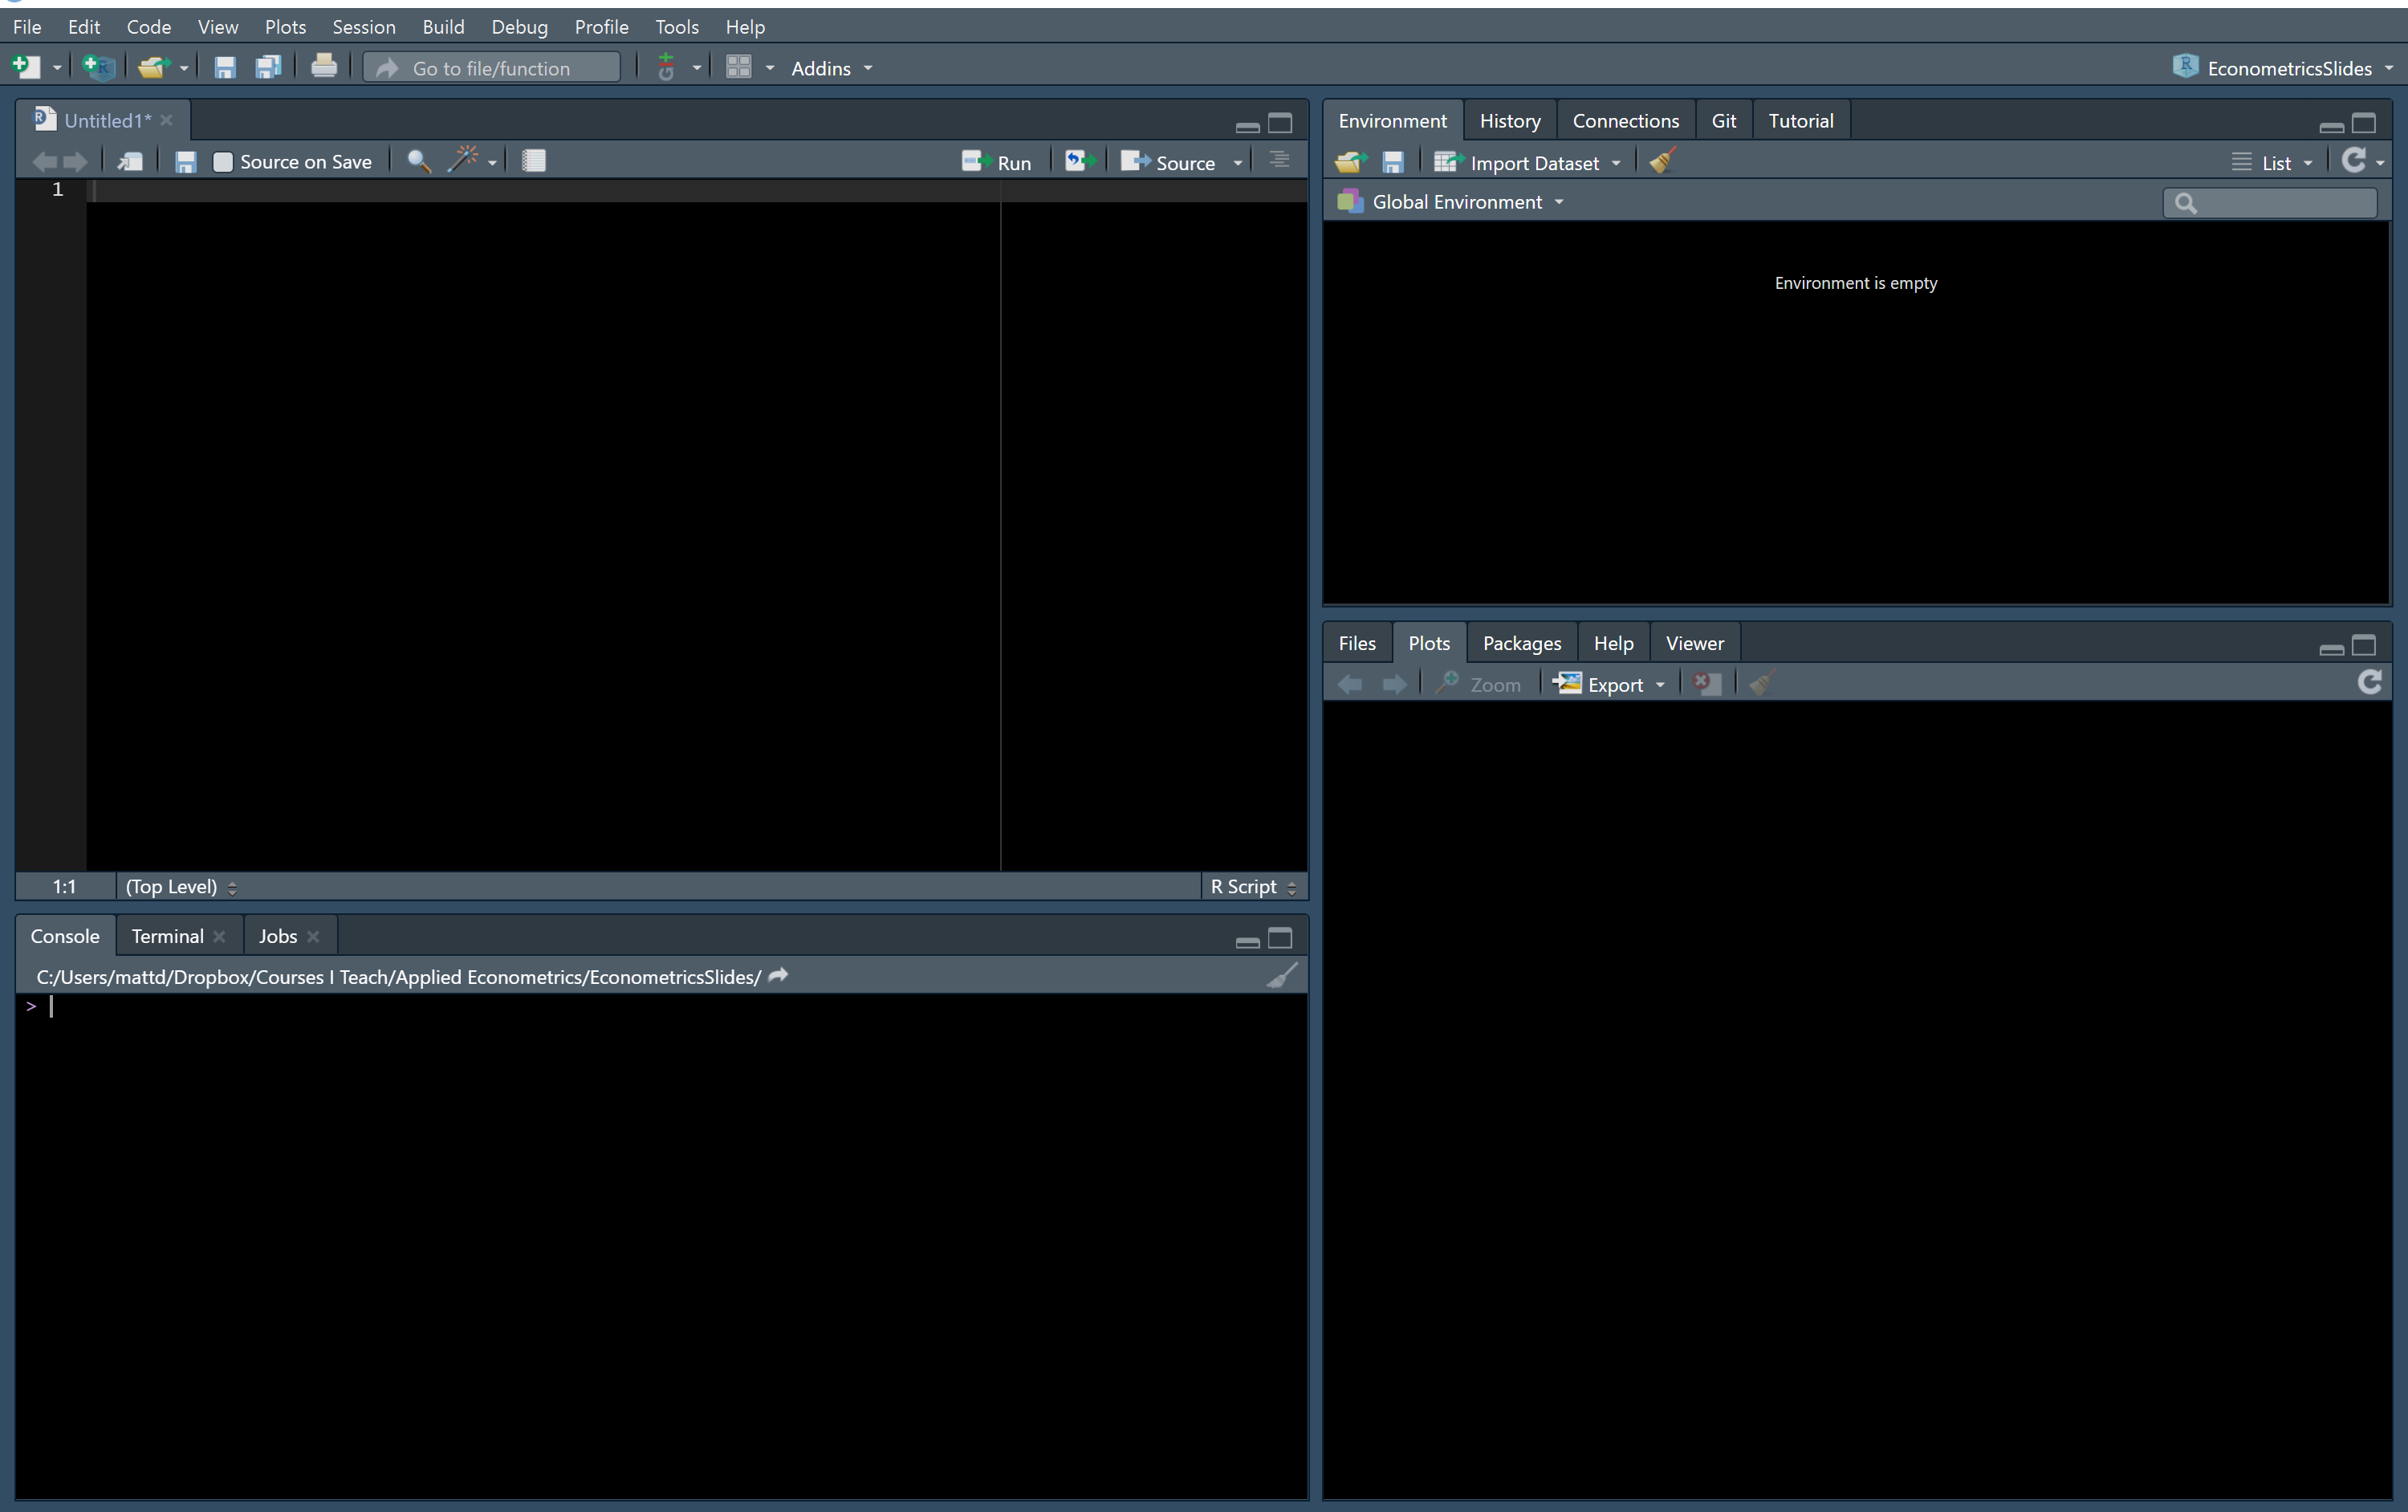
\includegraphics[width=1\linewidth,height=\textheight,keepaspectratio]{images/rstudiopanes.png}

\emph{Note: The layout in the image may look slightly different from
RStudio's default setup, but the differences are minor.}

\begin{tcolorbox}[enhanced jigsaw, colframe=quarto-callout-tip-color-frame, breakable, arc=.35mm, bottomtitle=1mm, bottomrule=.15mm, colbacktitle=quarto-callout-tip-color!10!white, rightrule=.15mm, colback=white, opacityback=0, opacitybacktitle=0.6, coltitle=black, left=2mm, toptitle=1mm, toprule=.15mm, titlerule=0mm, leftrule=.75mm, title=\textcolor{quarto-callout-tip-color}{\faLightbulb}\hspace{0.5em}{Tip from the Helpdesk: Pane Management}]

If you don't see four panes, don't worry! You can easily get them to
show up with the keyboard code Ctrl + Alt + Shift + 0 (Cmd + Alt + Shift
+ 0 on a Mac), or via the menu bar by clicking View \(\rightarrow\)
Panes \(\rightarrow\) Show All Panes.

That said, it's sometimes useful to minimize one or more of your panes.
When writing this book, for example, I typically only have the Editor
Pane and the Viewer Pane visible!

\end{tcolorbox}

\subsection{Bottom Left: The Console
Pane}\label{bottom-left-the-console-pane}

The console pane is where R lives. You can use R interactively here by
typing commands directly into the console. When you hit Enter, the
results are processed immediately. R is a command-line interpreter,
meaning it evaluates one command at a time as you type it.

However, most of your work will rely on scripts-sets of commands saved
in a file that are executed when you tell R to run them. Scripts ensure
your work is reproducible and organized. A typical R session will
include both interactive commands (quick tests, checks) and scripted
work for larger tasks. Scripts are housed in the editor pane.

\subsection{Top Left: The Editor Pane}\label{top-left-the-editor-pane}

This is where you will spend most of your time in RStudio. This is where
you write and save your scripts, which are sets of R commands that
RStudio can execute sequentially. You can run a whole script through the
console pane at once with the run button, or you can send one line at a
time to the console pane by selecting a line (or lines) by highlighting
them with your mouse and typing Ctrl-Enter (Cmd-Enter on Mac). Unlike
typing directly into the console, scripts allow you to save your work,
test code in sections, and reproduce your results later. You can have
multiple scripts or files open at once, each in its own tab, allowing
you to switch between tasks easily.

\begin{tcolorbox}[enhanced jigsaw, colframe=quarto-callout-tip-color-frame, breakable, arc=.35mm, bottomtitle=1mm, bottomrule=.15mm, colbacktitle=quarto-callout-tip-color!10!white, rightrule=.15mm, colback=white, opacityback=0, opacitybacktitle=0.6, coltitle=black, left=2mm, toptitle=1mm, toprule=.15mm, titlerule=0mm, leftrule=.75mm, title=\textcolor{quarto-callout-tip-color}{\faLightbulb}\hspace{0.5em}{Tip from the Helpdesk: Files Don't Save Themselves}]

If you see an asterisk (*) next to the name of a file on its tab, it
means the file has unsaved changes. Saving is like voting in Chicago;
one should do it early and often! Frequent saving will help you avoid
losing your work! You can save a file by clicking the Save icon or using
the shortcut Ctrl + S (Windows) or Cmd + S (Mac).

\end{tcolorbox}

If you're working with datasets loaded into memory, you can take a peek
at them in a spreadsheet-style view in the editor pane. This feature is
helpful for quickly inspecting your data and ensuring it looks as
expected. One way to do this is by using the \texttt{View()} command in
the console pane. For example, if you have a data frame called
\texttt{mydata}, typing \texttt{View(mydata)} in the console will
display the dataset in the editor window. Keep in mind, this viewer is
not a proper spreadsheet-you can't manually edit the data here. It's
purely for exploration and inspection.

RStudio also provides smart formatting in the editor pane to make
scripting easier, including:

\begin{itemize}
\tightlist
\item
  Color coding: Functions, variables, strings, and comments are visually
  distinct.
\item
  Bracket matching: Highlighted parentheses, braces, and brackets make
  it easier to spot mismatches.
\item
  Indentation: RStudio automatically aligns code blocks for better
  readability.
\item
  Code folding: Collapsible sections of code let you focus on specific
  parts of your script.
\end{itemize}

\subsection{Top Right: The Environment
Pane}\label{top-right-the-environment-pane}

The environment pane (top right) shows all the objects and variables
currently loaded into memory. This includes datasets, lists and vectors,
functions, and any other objects you create during your R session. For
example, if you load a dataset, its name will appear in this pane along
with information about its size and structure.

One particularly useful feature is the ability to click on a data frame
to open it in a spreadsheet-style view in the editor pane, making it
easy to examine your data visually--basically a shortcut for the
\texttt{View()} command discussed above. You can also see summaries of
objects (like the dimensions of a dataset or the class of an object)
without needing to type additional commands.

The environment pane also includes buttons and tools for managing your
workspace:

\begin{itemize}
\tightlist
\item
  Search Bar: Quickly locate specific objects in memory, which is
  especially useful when working with many variables.
\item
  Clear Workspace: The broom button will remove all objects from memory
  to start fresh (though use this with caution!).
\item
  Import Dataset Button: Launches a wizard to import data from external
  files (e.g.~CSV, Excel). This is a beginner-friendly way to learn how
  to load data into R.
\item
  List View vs.~Grid View: Toggle between a detailed list of objects and
  a more compact grid format.
\end{itemize}

Additionally, the environment pane interacts with RStudio projects,
which we will talk about later, displaying the workspace associated with
your current project. This ensures your work remains organized and makes
it easy to pick up where you left off.

Think of the environment pane as your workspace dashboard. It gives you
a clear view of everything you've created or loaded into R during your
session, helping you keep track of your data and variables as you work.

\subsection{Bottom Right: The Utility
Pane}\label{bottom-right-the-utility-pane}

The bottom right pane in RStudio is versatile and ultimately houses a
bunch of useful stuff that doesn't really fit with the vibe of the other
panes. It's kinda like a super organized junk drawer. The most commonly
used tabs include:

\begin{itemize}
\tightlist
\item
  Files: Browse your project's folder structure directly within RStudio.
  You can navigate to files, open scripts or datasets, and create new
  folders or files as needed.
\item
  Plots: View graphs and visualizations generated by your code. If you
  create multiple plots, RStudio allows you to scroll through them using
  the arrows in this tab. You can also export plots as image files
  (e.g., PNG or PDF) for use in reports or presentations.
\item
  Packages: Manage the R packages installed on your system. Packages are
  add-ons that extend R's functionality, providing specialized tools for
  specific tasks. You don't need to worry about the details yet, we'll
  cover packages and how to use them later in this chapter.
\item
  Help: Access R's built-in documentation. When you run a help command
  (e.g., \texttt{?lm}), the output will appear here. You can also search
  manually for functions, commands, or packages using the search bar.
\item
  Viewer: Used for displaying HTML outputs or other rendered content. In
  the Chapter on Literate Programming, Chapter~\ref{sec-litprog}, you'll
  see how this tab becomes important for viewing rendered reports or
  interactive documents.
\end{itemize}

The flexibility of the utility pane ensures that you can quickly access
the tools you need while working, whether that's managing files,
visualizing data, installing packages, or seeking help with R functions.

\subsection{Menu Bar}\label{menu-bar}

The menu bar is the last stop on our tour of the RStudio environment. It
contains options and commands typical of menu bars for most
programs--options like \emph{File}, \emph{Edit}, \emph{View},
\emph{Help}, etc. At some point you may want to look through these to
see what RStudio is capable of, but for now, here are a few useful
things to highlight.

\begin{itemize}
\tightlist
\item
  \emph{Code Menu}: Ensure the following 3 items are toggled on as they
  make reading and debugging your code easier.

  \begin{itemize}
  \tightlist
  \item
    Soft Wrap Long Lines: without this, long lines of code will have you
    scrolling horizontally for days!
  \item
    Rainbow Parentheses and Rainbow Fenced Divs: These options color
    match parentheses in different colors, making it much easier to see
    which opening parenthesis goes with which closing one. When your
    code gets complex with nested functions, this visual aid can save
    you from the frustration of hunting down mismatched parentheses.
  \end{itemize}
\item
  \emph{View Menu} \(\rightarrow\) \emph{Panes}: Here you can find an
  option to \emph{Show All Panes}. This is useful for situations where
  you accidentally close one of your four panes and want them back.
\item
  \emph{Help Menu} \(\rightarrow\) \emph{Cheatsheets}: RStudio provides
  a ton of coding cheatsheets that are incredibly useful for when you
  are trying to figure out how to do things. You can find a more
  comprehensive list of cheatsheets at
  \url{https://rstudio.com/resources/cheatsheets/}. Cheatsheets are
  designed to be printed out on a single double-sided sheet of paper and
  kept handy while working--you may find this especially valuable while
  learning new packages.
\item
  \emph{Help Menu} \(\rightarrow\) \emph{Keyboard Shortcuts Help}: As
  you code, you'll find that many repetitive tasks can be done more
  quickly and easily using keyboard shortcuts. RStudio provides this
  list of such shortcuts. At this point, looking at that list may be a
  bit daunting, but after you've become a bit more accustomed to using
  R, take a look at the list of keyboard shortcuts. You will likely find
  a few that you will soon view as indispensable. Here are the three I
  use the most:

  \begin{itemize}
  \tightlist
  \item
    Ctrl + Shift + M: This shortcut creates the pipe operator,
    \texttt{\textbar{}\textgreater{}}, which will be introduced in
    Chapter~\ref{sec-wrangling} on Data Wrangling.
  \item
    Ctrl + Alt + I: This key combination will create a new code chunk in
    Quarto, which we will discuss in Chapter~\ref{sec-litprog} Literate
    Programming.
  \item
    Ctrl + Shift + C: converts a line of script into a comment, useful
    for documenting scripts or temporarily ignoring lines when debugging
    code. More on this later this chapter.
  \end{itemize}
\item
  \emph{Tools Menu} \(\rightarrow\) \emph{Global Options}: This opens an
  options window with a variety of settings to customize RStudio. While
  most of the defaults are fine for you to start with, there are a few
  useful things to check out in here.

  \begin{itemize}
  \tightlist
  \item
    \emph{General Tab}: There is the option to set a \emph{Default
    working directory (when not in a project)}. Your working directory
    is simply the folder on your computer where R will look for files by
    default and where it will save output unless told otherwise. It's
    like R's ``home base'' on your computer. You should check out the
    Tip from the Helpdesk on RStudio Projects below, but I'd strongly
    suggest configuring this option right away. If, for example, you are
    using R as part of a class, create a folder on your hard drive for
    that class and set that folder as your working directory for R. Or,
    if you are simply teaching yourself R for fun, create a folder for
    learning R and set that as a working directory.
  \item
    \emph{Code Tab}: Ensure that \emph{Use native pipe operator,
    \textbar\textgreater{}} is ticked.
  \item
    \emph{Appearance Tab}: Here, you can set the theme of RStudio. If
    you want a dark theme, make sure you change the theme to ``Modern''
    or ``Sky''. I would suggest choosing a theme that has a lot of
    contrasting colors to make reading your code easier. You want the
    five colors of text in the sample display window to ``pop,'' because
    The different colors in the editor help you identify various parts
    of your code at a glance. I typically use Tomorrow Night Bright, but
    I also quite like Ambiance, Chaos, Cobalt, and Vibrant Ink.
  \item
    \emph{Packages Tab}: This enables you to determine where R looks to
    download packages--the community-developed functions and programs
    that greatly extend R's power. For the most part you want to ensure
    that the \emph{Primary CRAN repository} is set to \emph{Global (CDN)
    - RStudio}. If, however, you find yourself unable to install any
    packages, you will want to come back here and change your
    repository, likely to the repository closest to you geographically.
  \end{itemize}
\end{itemize}

\begin{tcolorbox}[enhanced jigsaw, colframe=quarto-callout-tip-color-frame, breakable, arc=.35mm, bottomtitle=1mm, bottomrule=.15mm, colbacktitle=quarto-callout-tip-color!10!white, rightrule=.15mm, colback=white, opacityback=0, opacitybacktitle=0.6, coltitle=black, left=2mm, toptitle=1mm, toprule=.15mm, titlerule=0mm, leftrule=.75mm, title=\textcolor{quarto-callout-tip-color}{\faLightbulb}\hspace{0.5em}{Tip from the Helpdesk: Projects: the Bento Boxes of R}]

Just as a bento box keeps your sushi separate from your tempura, RStudio
Projects keep your different coding tasks neatly compartmentalized. Each
project has its own workspace, history, and working directory, so your
econometrics homework won't mix with your data analysis for work. While
you might not need projects yet as you're just learning R, they become
invaluable when you're managing multiple research projects or juggling
different clients at work.

To create a project:

\begin{enumerate}
\def\labelenumi{\arabic{enumi}.}
\tightlist
\item
  Go to File \(\rightarrow\) New Project\ldots{}
\item
  Choose to create either a new folder or use an existing one
\item
  Give your project a name that helps you remember what it's for
\end{enumerate}

When you open a project, RStudio automatically puts you in the right
folder and loads the files you had open the last time you were working
on the project\ldots no more hunting around your computer for that
script you were working on last week!

For this book, consider creating a dedicated project called ``Learning
R'' or ``Econometrics'' to keep all your practice work organized in one
place.

\end{tcolorbox}

\section{R Essentials}\label{r-essentials}

With our whirlwind tour of RStudio out of the way, it's time to get our
hands dirty and start using R. For now, we have two choices for how we
use R (we will explore a third option in Chapter~\ref{sec-litprog}
Literate Programming). We can either:

\begin{enumerate}
\def\labelenumi{\arabic{enumi}.}
\tightlist
\item
  Type code directly into the console window (bottom left), or
\item
  Create an R Script by using \emph{File} \(\rightarrow\) \emph{New
  File} \(\rightarrow\) \emph{R Script}, enter our code into the script,
  and then manually run the lines from the script.
\end{enumerate}

While it sounds like option 1 is simpler, usually option 2 is the way to
go. Why? Scripts allow you to save your work, easily see what you've
already done, and make corrections to your code without retyping
everything. They are an essential tool for coding, and they make
learning easier as they provide a history of what you have already done.
At the end of the day:

\begin{itemize}
\tightlist
\item
  Scripting makes your work reproducible. You, or someone else, can
  re-run your code and get the same results.
\item
  Scripting makes it easier to work on a project over multiple sessions.
  You can easily pick up where you left off, even after a long break
\item
  Scripting helps you document your work. By adding comments (more on
  this below) to your code, you can explain your thought process,
  clarify complex sections, and make your script understandable for both
  your future self and others who might work with it.
\end{itemize}

\subsection{Code vs.~Comments}\label{code-vs.-comments}

A line in an R script will generally be one of two things--code, or a
comment.

\begin{itemize}
\tightlist
\item
  Code: A command or a set of instructions to tell the computer what to
  do
\item
  Comment: Notes that R will ignore entirely as it goes through your
  script
\end{itemize}

So, if R ignores comments, then what is their purpose?

Comments are something that you write for yourself, or people you are
working with. You may work on a script with another person who has no
idea what your code is all about, or you may not look at a script for a
few weeks and have forgotten what you were trying to accomplish! Putting
comments in your code is a way of making notes and passing them to
people with whom you are working and/or your future self.

It is easy to identify the difference between a line of code and a
comment in R--the hashtag symbol \texttt{\#} precedes a comment, and R
ignores anything on a line following a hashtag as well. You can see two
examples of comments in the code below:

\begin{Shaded}
\begin{Highlighting}[]
\CommentTok{\# This line is a comment!}
\DecValTok{2}\SpecialCharTok{+}\DecValTok{2} \CommentTok{\# This line has both code and a comment! }
\end{Highlighting}
\end{Shaded}

In the example above, the first line began with a \texttt{\#}, so R
would just ignore it and move on. The second line starts with code, and
R will read and execute everything in the line up until the \texttt{\#}
and then pretend like the rest of the line doesn't exist.

Comments are your way of documenting code, making it more understandable
and easier to share. For now, start practicing by adding simple comments
to your scripts as you learn, and concentrate on adding comments that
you think will help you make sense of your code later--what will the
future you want to know when you return to your script next week, next
month, or next year?

\subsection{Building Blocks of R: Objects and
Functions}\label{building-blocks-of-r-objects-and-functions}

While R is capable of being an incredibly elaborate calculator and doing
things like add \(2+2\), it is capable of much, much more than just
that. For the most part, everything you do in R fits into one of three
categories. You are either:

\begin{enumerate}
\def\labelenumi{\arabic{enumi}.}
\tightlist
\item
  Creating \emph{objects} (everything in R is an object),
\item
  Performing \emph{functions} on objects to create new objects or modify
  existing objects, or
\item
  Exploring and examining these objects to understand their structure or
  content.
\end{enumerate}

I will do my best to separate these three tasks in this section of the
book, but unfortunately, a clean separation is not entirely possible.
Some objects are created by functions, looking at objects requires you
to use functions, and so on.

\subsubsection{Objects}\label{objects}

\paragraph{Types of Objects}\label{types-of-objects}

Let's get started with basic object types and object assignment. At its
core, R is built around objects, which are like little boxes that hold
information. The three most fundamental object types in R are:

\begin{itemize}
\tightlist
\item
  Values: These are the simplest objects, holding a single piece of
  information (like the number \texttt{42}, or the word
  \texttt{France}).
\item
  Vectors: These are a collection of values, all of the same type (like
  a list of numbers: \texttt{1,\ 2,\ 3,\ 4}).
\item
  Data Frames: These are like tables or spreadsheets, where rows and
  columns hold different kinds of data.
\end{itemize}

We begin with the simplest object type, the value.

While using R you will spend a lot of time creating, defining, and
manipulating objects. The preferred way of creating an object is with
the assignment operator, \texttt{\textless{}-}. This is literally the
less than symbol \texttt{\textless{}} and a hyphen \texttt{-} slapped
together. The keyboard shortcut for the assignment operator is Alt +
\texttt{-} (Option + \texttt{-} on a Mac). While you technically can use
an equals sign (\texttt{=}) instead, that's generally frowned upon as
bad form in R programming. Let's start by creating an object \texttt{q}
and assigning to \texttt{q} the value 42 with the following code.

\begin{Shaded}
\begin{Highlighting}[]
\NormalTok{q }\OtherTok{\textless{}{-}} \DecValTok{42}
\end{Highlighting}
\end{Shaded}

You can verify that this worked by looking at the environment
window-recall, that's the top right pane. The first column tells you the
name of your object, \texttt{q}, and the second column shows you
something about that object. Because \texttt{q} is a numeric value
(technically, R would call this a numeric vector of length 1), R shows
you exactly what the value of \texttt{q} is: 42.

\begin{tcolorbox}[enhanced jigsaw, colframe=quarto-callout-tip-color-frame, breakable, arc=.35mm, bottomtitle=1mm, bottomrule=.15mm, colbacktitle=quarto-callout-tip-color!10!white, rightrule=.15mm, colback=white, opacityback=0, opacitybacktitle=0.6, coltitle=black, left=2mm, toptitle=1mm, toprule=.15mm, titlerule=0mm, leftrule=.75mm, title=\textcolor{quarto-callout-tip-color}{\faLightbulb}\hspace{0.5em}{Tip from the Helpdesk: Script it and Rip it}]

So, how do you make the assignment of \texttt{q\ \textless{}-\ 42}
happen? One option is to type that line of code into your console and
hit Enter. However, if you are taking my advice and doing this with a
script, you will have noticed that entering \texttt{q\ \textless{}-\ 42}
into your script and hitting Enter did nothing more remarkable than
simply advancing your cursor to the next line of your script.

There are a few ways to execute code from a script. The simplest
method--and the one I use most often--is to put your cursor on the line
of code you want to run in your script and hit Ctrl + Enter (Cmd + Enter
on a Mac) instead of just Enter. This is actually an example of a super
useful keyboard shortcut! Pressing Ctrl + Enter does two things; this
will \emph{both} advance your cursor to the next line of script
\emph{and} execute the line of code you just typed.

Alternately, if you look at the ribbon at the top of your script, you
will see a button that says \emph{Run}. You can use this button one of
two ways. You can either put your cursor on the line of code you want to
execute and click the button, which will run that line of code,
\emph{or} you can select a large chunk of code with your mouse (this can
be one line, multiple lines, or the whole script) and then click the
button. This will run every line of code you highlighted!

\end{tcolorbox}

Another way of verifying that \texttt{q} has a value of 42 is to simply
type \texttt{q} as a line of code.

\begin{Shaded}
\begin{Highlighting}[]
\NormalTok{q}
\end{Highlighting}
\end{Shaded}

\begin{verbatim}
[1] 42
\end{verbatim}

When you do this, R will return the value of \texttt{q}, here the number
\texttt{42}. Something that throws off many people when they start using
R is not realizing that everything in R is \emph{case-sensitive}. While
\texttt{q} is \texttt{42}, unless you have already assigned something to
\texttt{Q}, it will tell you there is an error:

\begin{Shaded}
\begin{Highlighting}[]
\NormalTok{Q}
\end{Highlighting}
\end{Shaded}

\begin{verbatim}
Error in eval(expr, envir, enclos): object 'Q' not found
\end{verbatim}

The error you see will likely be a little different (you should see
\texttt{Error:\ object\ \textquotesingle{}Q\textquotesingle{}\ not\ found"})
than what is printed here, but it will be an error nonetheless. As I
said, R takes being case-sensitive very seriously!

There are a couple simple rules that govern the naming of objects. The
only characters allowed in the name of an object are letters, numbers,
periods, or underscores, and object names must begin with a letter. I
could create objects with names like \texttt{q1}, \texttt{q.1} or
\texttt{q\_1}, but not something like \texttt{1q} (because it starts
with a number) or q!1 (because \texttt{!} is an invalid character).

\begin{Shaded}
\begin{Highlighting}[]
\NormalTok{q1 }\OtherTok{\textless{}{-}} \DecValTok{8675309}
\NormalTok{q}\FloatTok{.1} \OtherTok{\textless{}{-}} \FloatTok{2.718}
\NormalTok{q\_1 }\OtherTok{\textless{}{-}} \FloatTok{3.142}
\end{Highlighting}
\end{Shaded}

The fact that \texttt{q} is an object that contains the number
\texttt{42} will remain in R's memory until R is restarted, I overwrite
\texttt{q}, or I remove \texttt{q} (which we'll talk about when we get
to functions, a bit later). Overwriting a variable is easy; simply
assign a new value to an existing variable name:

\begin{Shaded}
\begin{Highlighting}[]
\NormalTok{q }\OtherTok{\textless{}{-}} \DecValTok{420}
\end{Highlighting}
\end{Shaded}

\begin{Shaded}
\begin{Highlighting}[]
\NormalTok{q}
\end{Highlighting}
\end{Shaded}

\begin{verbatim}
[1] 420
\end{verbatim}

Objects don't have to be be just numbers. They can hold character values
as well--essentially, words or text

\begin{Shaded}
\begin{Highlighting}[]
\NormalTok{a }\OtherTok{\textless{}{-}} \StringTok{"Hello World"}
\NormalTok{a}
\end{Highlighting}
\end{Shaded}

\begin{verbatim}
[1] "Hello World"
\end{verbatim}

Even though 1 is a number, wrapping it in quotation marks means R treats
it like a character value, not a numeric one.

\begin{Shaded}
\begin{Highlighting}[]
\NormalTok{b }\OtherTok{\textless{}{-}} \StringTok{"1"}
\end{Highlighting}
\end{Shaded}

A second important type of object is a \emph{vector}, a fancy, mathy
term for a list. To make a vector, we will need to use the
\textbf{concatenate} command \texttt{c()}. The next bit of code creates
two vectors, each with the first few numbers of a couple recognizable
sequences:

\begin{Shaded}
\begin{Highlighting}[]
\NormalTok{list\_squares }\OtherTok{\textless{}{-}} \FunctionTok{c}\NormalTok{(}\DecValTok{1}\NormalTok{, }\DecValTok{4}\NormalTok{, }\DecValTok{9}\NormalTok{, }\DecValTok{16}\NormalTok{, }\DecValTok{25}\NormalTok{, }\DecValTok{36}\NormalTok{, }\DecValTok{49}\NormalTok{)}
\NormalTok{list\_fib }\OtherTok{\textless{}{-}} \FunctionTok{c}\NormalTok{(}\DecValTok{1}\NormalTok{, }\DecValTok{1}\NormalTok{, }\DecValTok{2}\NormalTok{, }\DecValTok{3}\NormalTok{, }\DecValTok{5}\NormalTok{, }\DecValTok{8}\NormalTok{, }\DecValTok{13}\NormalTok{, }\DecValTok{21}\NormalTok{, }\DecValTok{35}\NormalTok{, }\DecValTok{56}\NormalTok{)}
\end{Highlighting}
\end{Shaded}

Vectors can also include characters:

\begin{Shaded}
\begin{Highlighting}[]
\NormalTok{countries }\OtherTok{\textless{}{-}} \FunctionTok{c}\NormalTok{(}\StringTok{"USA"}\NormalTok{, }\StringTok{"Canada"}\NormalTok{, }\StringTok{"Mexico"}\NormalTok{)}
\end{Highlighting}
\end{Shaded}

All the elements of a list have to be of the same type. This next bit of
code tries to create a list that has two values in it that are
characters and one value that is a number.

\begin{Shaded}
\begin{Highlighting}[]
\NormalTok{mixed\_list }\OtherTok{\textless{}{-}} \FunctionTok{c}\NormalTok{(}\StringTok{"Mt. Everest"}\NormalTok{, }\FloatTok{14.6}\NormalTok{, }\StringTok{"Armadillo"}\NormalTok{)}
\end{Highlighting}
\end{Shaded}

R will not allow this mixing of value types within a vector. It will
create the list, but it will force everything to be of the same type.
Since \texttt{"Mt.\ Everest"} and \texttt{"Armadillo"} cannot be forced
into being numbers, R will convert \texttt{14.6} to be a character.

The last of the fundamental object types to discuss is the data frame.
Typically, datasets in R exist in the form of a data frame. Think of a
data frame as being a table or a spreadsheet. Each individual column in
a data frame is like a vector, in that all of the values in that column
are required to be of the same type. A well structured data frame is
often described as \textbf{tidy data}, meaning that each row is a single
observation, and each column represents a different variable.

To make this more concrete, let's use an example. R contains a number of
inbuilt data frames for tutorial purposes, the most iconic of which is
the \texttt{iris} dataset. This data frame includes the measurements of
150 flowers--50 each from 3 different species of \emph{iris}. Let's go
ahead and load in the \texttt{iris} data frame with the command
\texttt{data(iris)}.

\begin{Shaded}
\begin{Highlighting}[]
\FunctionTok{data}\NormalTok{(iris)}
\end{Highlighting}
\end{Shaded}

For now, you should see \texttt{iris} show up in your Environment window
as a \emph{Value} with the rest of the objects you may have created so
far. You might notice that it lists the object contents as , which
simply means that R is waiting for you to actually do something with the
\texttt{iris} object before it actually loads the data in. This is fine,
this is done simply to conserve your computer's memory. As soon as you
start to work with the \texttt{iris} data, the object will move into the
\emph{Data} category in the Environment window, and you will see that it
has ``150 obs. of 5 variables,'' which means the dataset has 150 rows
and 5 columns.

When we get to functions later in this chapter, we will explore a wide
variety of ways to get more information about a data frame. At this
point, however, let's just take a quick look at what is in the
\texttt{iris} data with two functions, \texttt{str()} and
\texttt{head()}. The \emph{structure} function, \texttt{str()}, will
show us a bit of information about each variable, while \texttt{head()}
will print out the first six lines of data. These two functions combine
to give you a quick and useful snapshot of what the data look like
generally. Let's start with \texttt{head()}:

\begin{Shaded}
\begin{Highlighting}[]
\FunctionTok{head}\NormalTok{(iris)}
\end{Highlighting}
\end{Shaded}

\begin{verbatim}
  Sepal.Length Sepal.Width Petal.Length Petal.Width Species
1          5.1         3.5          1.4         0.2  setosa
2          4.9         3.0          1.4         0.2  setosa
3          4.7         3.2          1.3         0.2  setosa
4          4.6         3.1          1.5         0.2  setosa
5          5.0         3.6          1.4         0.2  setosa
6          5.4         3.9          1.7         0.4  setosa
\end{verbatim}

When you run \texttt{head()}, you'll see the first six rows of the
dataset printed in the console. Each row represents a single flower, and
each column corresponds to a specific feature or measurement of that
flower, such as \texttt{Petal.Length} or \texttt{Species}. This tidy
format-where rows are observations and columns are variables-makes the
iris dataset a great example of tidy data.

Next, looking at the structure allows us to learn a little more about
how each of the variables are stored:

\begin{Shaded}
\begin{Highlighting}[]
\FunctionTok{str}\NormalTok{(iris)}
\end{Highlighting}
\end{Shaded}

\begin{verbatim}
'data.frame':   150 obs. of  5 variables:
 $ Sepal.Length: num  5.1 4.9 4.7 4.6 5 5.4 4.6 5 4.4 4.9 ...
 $ Sepal.Width : num  3.5 3 3.2 3.1 3.6 3.9 3.4 3.4 2.9 3.1 ...
 $ Petal.Length: num  1.4 1.4 1.3 1.5 1.4 1.7 1.4 1.5 1.4 1.5 ...
 $ Petal.Width : num  0.2 0.2 0.2 0.2 0.2 0.4 0.3 0.2 0.2 0.1 ...
 $ Species     : Factor w/ 3 levels "setosa","versicolor",..: 1 1 1 1 1 1 1 1 1 1 ...
\end{verbatim}

Each row corresponds to one of the columns of the data frame, and next
to the column names, you can see the types of data that each column
contains. The first four variables, \texttt{Sepal.Length},
\texttt{Sepal.Width}, \texttt{Petal.Length}, and \texttt{Petal.Width},
are physical measurements of each flower and their type is listed as
\texttt{num}--a \emph{number}--which is pretty self explanatory! The
other variable, \texttt{Species}, is stored as a \emph{Factor}, which is
a special type of character value. It is a character in the sense that
it is not numeric, but R is also recognizing it as being categorical, so
it views, for example, all rows in which \(Species = "setosa"\) as being
part of the same group.

Here is a list of the most common variable types you will encounter in
R:

\begin{itemize}
\tightlist
\item
  Number: Sometimes you will see \texttt{num}, sometimes these are
  listed as \texttt{dbl}, or \emph{double}. Doubles are are just numbers
  that can have decimal values.
\item
  Factor: Often shortened as \texttt{fctr}, a factor is a character
  value where R recognizes the variable as being categorical.
\item
  Character: These can be abbreviated as \texttt{chr}. A character value
  where R does not recognize the variable as being categorical.
\item
  Logical: In shorthand \texttt{lgl}, a logical variable is one where
  the only two possible values are \texttt{TRUE} and \texttt{FALSE}.
\end{itemize}

\paragraph{Subsetting and Extracting From
Objects}\label{subsetting-and-extracting-from-objects}

We often want to extract elements from our objects. In the case of a
value, it is simple, as it only has one element. If we want to know what
\texttt{q} is, we can simply refer to it as \texttt{q}. Extracting
elements from vectors and data frames is a bit trickier, and requires us
to use brackets (\texttt{{[}{]}}) for subsetting.

We will start with extracting elements from a vector.

Element extraction is extremely powerful and useful in R. Understanding
this first requires an understanding of \emph{indexing}, which
essentially refers to the position of an element in an object; the first
element of any object is at index position 1, the second element is at
index position 2, and so forth.

The following commands extracts the fourth element from
\texttt{list\_squares} (the fourth square number is 16) and the sixth
element from \texttt{list\_fib} (the 6th number in the Fibonacci
sequence is 8):

\begin{Shaded}
\begin{Highlighting}[]
\NormalTok{list\_squares[}\DecValTok{4}\NormalTok{] }
\end{Highlighting}
\end{Shaded}

\begin{verbatim}
[1] 16
\end{verbatim}

\begin{Shaded}
\begin{Highlighting}[]
\NormalTok{list\_fib[}\DecValTok{6}\NormalTok{]}
\end{Highlighting}
\end{Shaded}

\begin{verbatim}
[1] 8
\end{verbatim}

We can extract all but certain elements with the negative sign; this is
called negative indexing. Let's see \texttt{list\_squares} without the
third element:

\begin{Shaded}
\begin{Highlighting}[]
\NormalTok{list\_squares[}\SpecialCharTok{{-}}\DecValTok{3}\NormalTok{]}
\end{Highlighting}
\end{Shaded}

\begin{verbatim}
[1]  1  4 16 25 36 49
\end{verbatim}

Another technique is to pull a specific subset. Say we want the 3rd
through 6th element of the \texttt{list\_squares} vector. The colon
operator (:) generates a sequence of numbers from the first to the last
number, inclusive. In this case, 3:6 creates the sequence 3, 4, 5, 6,
allowing you to extract these specific elements.

\begin{Shaded}
\begin{Highlighting}[]
\NormalTok{list\_squares[}\DecValTok{3}\SpecialCharTok{:}\DecValTok{6}\NormalTok{]}
\end{Highlighting}
\end{Shaded}

\begin{verbatim}
[1]  9 16 25 36
\end{verbatim}

A very common use of this functionality is to extract based on a
condition, or \emph{filter} your data. Filtering is very useful when
working with large datasets, or trying to work with specific subsets of
a larger data set. For example, the next command will extract all the
elements of \texttt{list\_fib} that are greater than 10:

\begin{Shaded}
\begin{Highlighting}[]
\NormalTok{list\_fib[list\_fib}\SpecialCharTok{\textgreater{}}\DecValTok{10}\NormalTok{]}
\end{Highlighting}
\end{Shaded}

\begin{verbatim}
[1] 13 21 35 56
\end{verbatim}

Filtering like this is a bit trickier than simply using indexes because
of the use of the comparison operator to evaluate whether each element
in \texttt{list\_fib} is greater than 10. The most common comparison
operators in R are:

\begin{itemize}
\tightlist
\item
  \texttt{\textgreater{}}: Greater than
\item
  \texttt{\textless{}}: Less than
\item
  \texttt{\textgreater{}=}: Greater than or equal to
\item
  \texttt{\textless{}=}: Less than or equal to
\item
  \texttt{!=}: Not equal to
\item
  \texttt{==}: Equal to
\end{itemize}

The \texttt{==} comparator is probably the trickiest one to wrap your
mind around; note the double equals sign! To differentiate between
\texttt{=} and \texttt{==}, I like to read \texttt{=} as ``is'' or
``equals'' and \texttt{==} as ``is equal to''. This mental distinction
is usually pretty good for helping me determine which symbol to use, as
it helps clarify that \texttt{==} is used when comparing values.

Extracting elements from a data frame is decidely more complex than from
a vector because you need to specify both rows and columns. That said,
most of the techniques found above in the vector subsetting section work
here. The general syntax for subsetting a data frame is
\texttt{dataframe{[}row,\ column{]}}

\begin{itemize}
\tightlist
\item
  The number before the comma refers to the row(s) you want to extract.
\item
  The number after the comma refers to the column(s) you want to
  extract.
\item
  Leaving one of these blank will include all rows or all columns,
  respectively.
\end{itemize}

Let's turn back to the \texttt{iris} dataset for some concrete examples.

Suppose we want to extract the value in the third row and fifth column,
which corresponds to the species of the third flower:

\begin{Shaded}
\begin{Highlighting}[]
\NormalTok{iris[}\DecValTok{3}\NormalTok{, }\DecValTok{5}\NormalTok{]}
\end{Highlighting}
\end{Shaded}

\begin{verbatim}
[1] setosa
Levels: setosa versicolor virginica
\end{verbatim}

You can extract an entire row or column by leaving one of the indices
blank. Let's extract the entire 73rd row:

\begin{Shaded}
\begin{Highlighting}[]
\NormalTok{iris[}\DecValTok{73}\NormalTok{, ]}
\end{Highlighting}
\end{Shaded}

\begin{verbatim}
   Sepal.Length Sepal.Width Petal.Length Petal.Width    Species
73          6.3         2.5          4.9         1.5 versicolor
\end{verbatim}

And now, the entire third column (\texttt{Petal.Length}):

\begin{Shaded}
\begin{Highlighting}[]
\NormalTok{iris[, }\DecValTok{3}\NormalTok{]}
\end{Highlighting}
\end{Shaded}

\begin{verbatim}
  [1] 1.4 1.4 1.3 1.5 1.4 1.7 1.4 1.5 1.4 1.5 1.5 1.6 1.4 1.1 1.2 1.5 1.3 1.4
 [19] 1.7 1.5 1.7 1.5 1.0 1.7 1.9 1.6 1.6 1.5 1.4 1.6 1.6 1.5 1.5 1.4 1.5 1.2
 [37] 1.3 1.4 1.3 1.5 1.3 1.3 1.3 1.6 1.9 1.4 1.6 1.4 1.5 1.4 4.7 4.5 4.9 4.0
 [55] 4.6 4.5 4.7 3.3 4.6 3.9 3.5 4.2 4.0 4.7 3.6 4.4 4.5 4.1 4.5 3.9 4.8 4.0
 [73] 4.9 4.7 4.3 4.4 4.8 5.0 4.5 3.5 3.8 3.7 3.9 5.1 4.5 4.5 4.7 4.4 4.1 4.0
 [91] 4.4 4.6 4.0 3.3 4.2 4.2 4.2 4.3 3.0 4.1 6.0 5.1 5.9 5.6 5.8 6.6 4.5 6.3
[109] 5.8 6.1 5.1 5.3 5.5 5.0 5.1 5.3 5.5 6.7 6.9 5.0 5.7 4.9 6.7 4.9 5.7 6.0
[127] 4.8 4.9 5.6 5.8 6.1 6.4 5.6 5.1 5.6 6.1 5.6 5.5 4.8 5.4 5.6 5.1 5.1 5.9
[145] 5.7 5.2 5.0 5.2 5.4 5.1
\end{verbatim}

To extract a specific subset of rows and columns, specify both indices.
For example, let's extract rows 1--3 and columns 1--2 (Sepal.Length and
Sepal.Width):

\begin{Shaded}
\begin{Highlighting}[]
\NormalTok{iris[}\DecValTok{1}\SpecialCharTok{:}\DecValTok{3}\NormalTok{, }\DecValTok{1}\SpecialCharTok{:}\DecValTok{2}\NormalTok{]}
\end{Highlighting}
\end{Shaded}

\begin{verbatim}
  Sepal.Length Sepal.Width
1          5.1         3.5
2          4.9         3.0
3          4.7         3.2
\end{verbatim}

Things get tricker when we want to filter specific rows or columns.
Filtering rows based on a condition is similar to subsetting vectors but
applied to the rows of the data frame. Suppose we want to just look at
the \texttt{versicolor} irises.

\begin{Shaded}
\begin{Highlighting}[]
\NormalTok{iris[iris}\SpecialCharTok{$}\NormalTok{Species }\SpecialCharTok{==} \StringTok{"versicolor"}\NormalTok{, ]}
\end{Highlighting}
\end{Shaded}

\begin{verbatim}
    Sepal.Length Sepal.Width Petal.Length Petal.Width    Species
51           7.0         3.2          4.7         1.4 versicolor
52           6.4         3.2          4.5         1.5 versicolor
53           6.9         3.1          4.9         1.5 versicolor
54           5.5         2.3          4.0         1.3 versicolor
55           6.5         2.8          4.6         1.5 versicolor
56           5.7         2.8          4.5         1.3 versicolor
57           6.3         3.3          4.7         1.6 versicolor
58           4.9         2.4          3.3         1.0 versicolor
59           6.6         2.9          4.6         1.3 versicolor
60           5.2         2.7          3.9         1.4 versicolor
61           5.0         2.0          3.5         1.0 versicolor
62           5.9         3.0          4.2         1.5 versicolor
63           6.0         2.2          4.0         1.0 versicolor
64           6.1         2.9          4.7         1.4 versicolor
65           5.6         2.9          3.6         1.3 versicolor
66           6.7         3.1          4.4         1.4 versicolor
67           5.6         3.0          4.5         1.5 versicolor
68           5.8         2.7          4.1         1.0 versicolor
69           6.2         2.2          4.5         1.5 versicolor
70           5.6         2.5          3.9         1.1 versicolor
71           5.9         3.2          4.8         1.8 versicolor
72           6.1         2.8          4.0         1.3 versicolor
73           6.3         2.5          4.9         1.5 versicolor
74           6.1         2.8          4.7         1.2 versicolor
75           6.4         2.9          4.3         1.3 versicolor
76           6.6         3.0          4.4         1.4 versicolor
77           6.8         2.8          4.8         1.4 versicolor
78           6.7         3.0          5.0         1.7 versicolor
79           6.0         2.9          4.5         1.5 versicolor
80           5.7         2.6          3.5         1.0 versicolor
81           5.5         2.4          3.8         1.1 versicolor
82           5.5         2.4          3.7         1.0 versicolor
83           5.8         2.7          3.9         1.2 versicolor
84           6.0         2.7          5.1         1.6 versicolor
85           5.4         3.0          4.5         1.5 versicolor
86           6.0         3.4          4.5         1.6 versicolor
87           6.7         3.1          4.7         1.5 versicolor
88           6.3         2.3          4.4         1.3 versicolor
89           5.6         3.0          4.1         1.3 versicolor
90           5.5         2.5          4.0         1.3 versicolor
91           5.5         2.6          4.4         1.2 versicolor
92           6.1         3.0          4.6         1.4 versicolor
93           5.8         2.6          4.0         1.2 versicolor
94           5.0         2.3          3.3         1.0 versicolor
95           5.6         2.7          4.2         1.3 versicolor
96           5.7         3.0          4.2         1.2 versicolor
97           5.7         2.9          4.2         1.3 versicolor
98           6.2         2.9          4.3         1.3 versicolor
99           5.1         2.5          3.0         1.1 versicolor
100          5.7         2.8          4.1         1.3 versicolor
\end{verbatim}

You may have noticed that the complexity just ramped up with that last
line of code! A few things need to be explained:

\begin{itemize}
\item
  The ``\,'' around \texttt{versicolor} indicate that
  \texttt{versicolor} is a character string. In R, text values (also
  called character values) must always be wrapped in either single (')
  or double (``) quotation marks to differentiate them from object
  names, numeric values, or commands. Without the quotes, R would think
  you were referring to an object named versicolor, which doesn't exist
  unless you've defined it earlier.
\item
  The \$ operator is used to refer to a specific column within a data
  frame by its name, rather than by its index position. Think of it as
  saying, ``Hey, R, show me just this column.'' In this case,
  iris\$Species pulls out the Species column from the iris data frame,
  which contains the species classification for each flower.
\item
  After the condition (\texttt{iris\$Species\ ==\ "versicolor"}),
  there's a comma followed by nothing. This syntax tells R to filter
  rows based on the condition, but keep all columns. If we wanted to
  filter specific rows and specific columns, we'd include an additional
  condition after the comma.
\end{itemize}

The key difference between subsetting vectors and data frames is that,
when extracting elements or filtering data frames, remember that you
must specify both rows and columns. This added complexity makes data
frame subsetting more powerful but also trickier than working with
vectors.

Subsetting and extracting elements from data frames is a powerful skill
that allows you to focus on specific parts of your data, whether by
selecting rows, columns, or filtering based on conditions. These
techniques are essential for data analysis and are widely applicable
across various projects.

In Chapter~\ref{sec-wrangling} on Data Wrangling, we'll explore the
\textbf{Tidyverse}, a set of R add-ons designed to make working with
data more intuitive. I personally prefer the Tidyverse, and we will make
more use if it throughout the text than the methogs above. The Tidyverse
introduces methods for subsetting and extracting data that most people
find easier to learn and use, especially with larger datasets or more
complex operations. That said, it's still worth learning these
foundational techniques. Even as the Tidyverse simplifies and
streamlines many tasks, understanding these basics will give you greater
insight into how R works and will be invaluable when you encounter
situations where Tidyverse tools might not be the best fit.

\subsubsection{Functions}\label{functions}

Let's talk about functions! Functions are the heavy lifters of R-they
handle most of the actual work in your scripts, and using them is the
key to nearly everything you will do in R. In this section, we'll break
down what functions are, how they work, and why they're so important.
I'll also introduce a few super useful functions to get you started, but
the goal here isn't to take a deep dive into specific functions.
Instead, we're focusing on the big picture: understanding how functions
operate so you can use them effectively.

Functions are how we get R to do things. They take input, process it,
and (usually) give us some output. Functions are so central to R that
you've already used some-commands like \texttt{head()}, \texttt{str()},
and \texttt{data()} are all functions!

One of the first functions to know is rm(), which stands for ``remove.''
This handy function lets you delete objects from your environment when
they're no longer needed. Do you no longer need \texttt{q}?

\begin{Shaded}
\begin{Highlighting}[]
\FunctionTok{rm}\NormalTok{(q)}
\end{Highlighting}
\end{Shaded}

Poof! It's gone. Do you want a reset button? Get rid of all the objects
in your environment? This is a bit of a trickier command, but:

\begin{Shaded}
\begin{Highlighting}[]
\FunctionTok{rm}\NormalTok{(}\AttributeTok{list =} \FunctionTok{ls}\NormalTok{())}
\end{Highlighting}
\end{Shaded}

Be careful with this one; it's the nuclear option!

Beyond \texttt{head()} and \texttt{str()}, there are a few useful tools
for exploring your data:

\begin{itemize}
\tightlist
\item
  \texttt{View()}: Opens your data frame in a spreadsheet-style viewer.
  Great for getting a bird's-eye view.
\item
  \texttt{summary()}: Provides basic summary statistics for each column
  in a data frame. Perfect for a quick look at your data's distribution.
  This function has a lot of other uses for other object types as well;
  we will look at them later.
\item
  \texttt{class()}: Tells you the data type of an object. Is it a
  vector? A data frame? Something else? You can also feed a particular
  column into \texttt{class()} to learn about the type of variable it
  is.
\item
  \texttt{names()}: Returns a list of the variable names in a dataset.
  This also has a lot of uses for different object types.
\item
  \texttt{levels()}: Useful for exploring factors (categorical
  variables). This shows you the categories that exist in a factor
  variable.
\end{itemize}

Let's use some of these new functions with the \texttt{iris} data set.
But first, since I just nuked my workspace with
\texttt{rm(list\ =\ ls())}, I need to get it back!

\begin{Shaded}
\begin{Highlighting}[]
\FunctionTok{data}\NormalTok{(iris)}
\end{Highlighting}
\end{Shaded}

The results of \texttt{View(iris)} won't show up in this document,
because technically, \texttt{View()} is not an R command, it's an
RStudio only command. If you execute the line of code below, you should
see a spreadsheet-like view of the dataset pop up in your Editor pane.
While \texttt{View()} is very useful in small datasets, when you start
to encounter massive ones \texttt{View()} can get sluggish.

\begin{Shaded}
\begin{Highlighting}[]
\FunctionTok{View}\NormalTok{(iris)}
\end{Highlighting}
\end{Shaded}

We can get a brief overview of some of the summary statistics of the
data with the \texttt{summary()} function:

\begin{Shaded}
\begin{Highlighting}[]
\FunctionTok{summary}\NormalTok{(iris)}
\end{Highlighting}
\end{Shaded}

\begin{verbatim}
  Sepal.Length    Sepal.Width     Petal.Length    Petal.Width   
 Min.   :4.300   Min.   :2.000   Min.   :1.000   Min.   :0.100  
 1st Qu.:5.100   1st Qu.:2.800   1st Qu.:1.600   1st Qu.:0.300  
 Median :5.800   Median :3.000   Median :4.350   Median :1.300  
 Mean   :5.843   Mean   :3.057   Mean   :3.758   Mean   :1.199  
 3rd Qu.:6.400   3rd Qu.:3.300   3rd Qu.:5.100   3rd Qu.:1.800  
 Max.   :7.900   Max.   :4.400   Max.   :6.900   Max.   :2.500  
       Species  
 setosa    :50  
 versicolor:50  
 virginica :50  
                
                
                
\end{verbatim}

For the \texttt{iris} data, it creates numerical summary statistics of
the 4 numeric variables and a tabulation of the categorical variable.

Next, we can see the result of the \texttt{class()} function:

\begin{Shaded}
\begin{Highlighting}[]
\FunctionTok{class}\NormalTok{(iris)}
\end{Highlighting}
\end{Shaded}

\begin{verbatim}
[1] "data.frame"
\end{verbatim}

This is not that useful. Where \texttt{class()} shines with data is when
you look for the class of a variable:

\begin{Shaded}
\begin{Highlighting}[]
\FunctionTok{class}\NormalTok{(iris}\SpecialCharTok{$}\NormalTok{Species)}
\end{Highlighting}
\end{Shaded}

\begin{verbatim}
[1] "factor"
\end{verbatim}

The \texttt{levels()} function is really useful when looking at factor
variables--knowing the variable is categorical is good, but what if you
want to know what the possible values for your factor variable are? This
is where \texttt{levels()} comes in handy:

\begin{Shaded}
\begin{Highlighting}[]
\FunctionTok{levels}\NormalTok{(iris}\SpecialCharTok{$}\NormalTok{Species)}
\end{Highlighting}
\end{Shaded}

\begin{verbatim}
[1] "setosa"     "versicolor" "virginica" 
\end{verbatim}

Functions often have more than one input, called arguments, that let you
customize what the function does. Let's look at an example using the
\texttt{round()} function, a fairly simple function which rounds numbers
to a specified number of decimal places. The syntax for round() is
\texttt{round(x,\ digits)}, where \texttt{x} is what you want to round
and \texttt{digits} is the number of decimal places to round to.

Let's work with a couple examples to see how this works. Let's create an
object called \texttt{pi} that is the mathematical constant \(\pi\) to
10 decimal places.

\begin{Shaded}
\begin{Highlighting}[]
\NormalTok{pi }\OtherTok{\textless{}{-}} \FloatTok{3.1415926535}
\end{Highlighting}
\end{Shaded}

The ``proper'' way to specify arguments is with the \texttt{=} sign, so
we might round \texttt{pi} to three decimal places by typing:

\begin{Shaded}
\begin{Highlighting}[]
\FunctionTok{round}\NormalTok{(}\AttributeTok{x =}\NormalTok{ pi, }\AttributeTok{digits =} \DecValTok{3}\NormalTok{)}
\end{Highlighting}
\end{Shaded}

\begin{verbatim}
[1] 3.142
\end{verbatim}

If we are going to do it the ``proper'' way, then it doesn't matter
which order we put our arguments. Note that reversing the order of the
arguments gives the same result:

\begin{Shaded}
\begin{Highlighting}[]
\FunctionTok{round}\NormalTok{(}\AttributeTok{digits =} \DecValTok{3}\NormalTok{, }\AttributeTok{x =}\NormalTok{ pi)}
\end{Highlighting}
\end{Shaded}

\begin{verbatim}
[1] 3.142
\end{verbatim}

Once you become more accustomed to specific functions, and you learn the
default order of the arguments, you can dispense with the \texttt{x\ =}
and \texttt{digits\ =} and just enter the arguments directly into the
function. If you do this, R assumes that we are putting our arguments
into the function in the order of \texttt{(x,\ digits)}, so the easiest
way to round \texttt{pi} to 3 decimal places is:

\begin{Shaded}
\begin{Highlighting}[]
\FunctionTok{round}\NormalTok{(pi, }\DecValTok{3}\NormalTok{)}
\end{Highlighting}
\end{Shaded}

\begin{verbatim}
[1] 3.142
\end{verbatim}

Strictly speaking, the \texttt{digits} is an \emph{optional} argument;
you can specify a number of places to round to, but if you don't, there
is a default value pre-programmed into R. In this case, the default
value is 0. If I want \texttt{pi} rounded to the nearest whole number, I
could type:

\begin{Shaded}
\begin{Highlighting}[]
\FunctionTok{round}\NormalTok{(pi)}
\end{Highlighting}
\end{Shaded}

\begin{verbatim}
[1] 3
\end{verbatim}

\begin{tcolorbox}[enhanced jigsaw, colframe=quarto-callout-tip-color-frame, breakable, arc=.35mm, bottomtitle=1mm, bottomrule=.15mm, colbacktitle=quarto-callout-tip-color!10!white, rightrule=.15mm, colback=white, opacityback=0, opacitybacktitle=0.6, coltitle=black, left=2mm, toptitle=1mm, toprule=.15mm, titlerule=0mm, leftrule=.75mm, title=\textcolor{quarto-callout-tip-color}{\faLightbulb}\hspace{0.5em}{Tip}]

\#\#\#\#\#\#Tip from the Helpdesk: Parental Advisory Explicit Content

When should you use the \texttt{=} sign to specify arguments explicitly?
It really depends on the situation:

\begin{itemize}
\item
  Be Explicit: If you're new to a function or sharing your code with
  others, using = makes your intentions crystal clear. For example,
  \texttt{round(x\ =\ pi,\ digits\ =\ 3)} leaves no doubt about what
  you're doing, even to someone seeing the code for the first time.
  Explicit arguments also prevent mistakes when functions have many
  inputs, or when you're skipping over optional arguments. This is
  especially helpful if you only want to change one or two specific
  arguments from their default values while leaving the rest untouched.
\item
  Skip the Explicitness: Once you've mastered a function and know its
  argument order by heart, you can skip the = for a quicker, cleaner
  look. For instance, \texttt{round(pi,\ 3)} works just as well and is
  easier to read when the function is simple and the meaning is obvious.
\end{itemize}

Ultimately, the choice between explicit and implicit argument calling
depends on your context. I suggest that you prioritize clarity and
explicitness when learning, debugging, or sharing code. As you gain
experience and familiarity with functions, you can adopt a more
streamlined approach for speed and simplicity. Find what works best for
you!

\end{tcolorbox}

A final useful bit to note: you will often want to save the output of a
function as an object. This can be done with the assignment operator.
For example:

\begin{Shaded}
\begin{Highlighting}[]
\NormalTok{pi3 }\OtherTok{\textless{}{-}} \FunctionTok{round}\NormalTok{(pi, }\DecValTok{3}\NormalTok{)}
\end{Highlighting}
\end{Shaded}

This creates an object called \texttt{pi3} that is \texttt{pi} rounded
to three decimal places. Note that creating the object doesn't create
any output! However, you should be able to see \texttt{pi3} in your
environment window, and I can use it in my code if I want:

\begin{Shaded}
\begin{Highlighting}[]
\NormalTok{pi3}
\end{Highlighting}
\end{Shaded}

\begin{verbatim}
[1] 3.142
\end{verbatim}

So, let's stretch our legs a bit and combine some of the techniques
we've seen thus far. Suppose we want to calculate the average petal
length for each of the three different iris types, and to save each of
these averages as an object. How might we do this? We need one function
that we haven't seen yet, the \texttt{mean()} function, but the rest of
this task can be accomplished with what we've learned so far. We'll use
the mean() function to calculate the average, combined with subsetting
and filtering techniques to isolate each species. For example, this line
of code will calculate the mean petal length of setosa irises and put it
into the object \texttt{mean\_setosa}:

\begin{Shaded}
\begin{Highlighting}[]
\NormalTok{mean\_setosa }\OtherTok{\textless{}{-}} \FunctionTok{mean}\NormalTok{(iris}\SpecialCharTok{$}\NormalTok{Petal.Length[iris}\SpecialCharTok{$}\NormalTok{Species }\SpecialCharTok{==} \StringTok{"setosa"}\NormalTok{])}
\end{Highlighting}
\end{Shaded}

How does this work?

\begin{itemize}
\tightlist
\item
  \texttt{iris\$Petal.Length}: This selects the Petal.Length column from
  the iris dataset.
\item
  \texttt{{[}iris\$Species\ ==\ "setosa"{]}}: This subsets the
  Petal.Length column to include only the rows where the species is
  setosa.
\item
  \texttt{mean()}: This calculates the average of the subsetted petal
  lengths.
\item
  Assignment with \texttt{\textless{}-}: Finally, we assign the
  calculated mean to a new object called \texttt{mean\_setosa}.
\end{itemize}

How would you go about calculating the means of the versicolor and
virginica irises? Think about it, then check the answer below:

\begin{Shaded}
\begin{Highlighting}[]
\NormalTok{mean\_versicolor }\OtherTok{\textless{}{-}} \FunctionTok{mean}\NormalTok{(iris}\SpecialCharTok{$}\NormalTok{Petal.Length[iris}\SpecialCharTok{$}\NormalTok{Species }\SpecialCharTok{==} \StringTok{"versicolor"}\NormalTok{])}
\NormalTok{mean\_virginica }\OtherTok{\textless{}{-}} \FunctionTok{mean}\NormalTok{(iris}\SpecialCharTok{$}\NormalTok{Petal.Length[iris}\SpecialCharTok{$}\NormalTok{Species }\SpecialCharTok{==} \StringTok{"virginica"}\NormalTok{])}
\end{Highlighting}
\end{Shaded}

If I told you that the function to calculate a standard deviation was
\texttt{sd()}, do you think you could repeat this task for the standard
deviation for each iris type?

\begin{tcolorbox}[enhanced jigsaw, colframe=quarto-callout-tip-color-frame, breakable, arc=.35mm, bottomtitle=1mm, bottomrule=.15mm, colbacktitle=quarto-callout-tip-color!10!white, rightrule=.15mm, colback=white, opacityback=0, opacitybacktitle=0.6, coltitle=black, left=2mm, toptitle=1mm, toprule=.15mm, titlerule=0mm, leftrule=.75mm, title=\textcolor{quarto-callout-tip-color}{\faLightbulb}\hspace{0.5em}{Tip from the Helpdesk: Help! I Need Somebody!}]

Stuck on a function? Encountered an error that makes no sense? Welcome
to programming-this happens to everyone. Here are some strategies to get
unstuck:

\begin{itemize}
\item
  Read the Error Message: The error messages in R often feel cryptic at
  first, but they usually contain valuable clues. Carefully read the
  error message and pay attention to the function or object it mentions.
  For example,
  \texttt{Error\ in\ mean(x)\ :\ \textquotesingle{}x\textquotesingle{}\ must\ be\ numeric}
  is telling you that there is a mismatch between what the function
  \texttt{mean(x)} wants you to use as an argument and what you actually
  used as an argument. Or, in English, you are trying to calculate the
  average of something that isn't a set of numbers!
\item
  Google It: If the error message doesn't make sense, copy and paste it
  into Google (or your search engine of choice). Chances are, someone
  else has encountered the exact same issue before. Include ``R'' in
  your search query to narrow results to relevant discussions.
\item
  Search Discussion Boards: Websites like Stack Overflow are goldmines
  for R troubleshooting. Search the error message, function name, or
  problem description-many questions have already been asked and
  answered. If you don't find an exact match, consider posting your
  question (and include a clear explanation with reproducible code!).
\item
  Check R's Built-In Help: Use \texttt{?function\_name} (e.g.,
  \texttt{?sd}) or \texttt{help(function\_name)} in the console to
  access R's documentation for a function. While this can be dense, it
  often includes examples that can clarify how a function works.
\item
  Experiment and Simplify: If the error seems mysterious, try breaking
  your code into smaller chunks and running them one by one. This can
  help pinpoint where things are going wrong.
\item
  Ask for Help (Politely): If all else fails, reach out to someone
  knowledgeable, such as a colleague, professor, or online community.
  When asking for help, provide context, include the full error message,
  and share your code (or a simplified version of it). Clear questions
  get faster, more helpful answers.
\end{itemize}

Remember, troubleshooting is an essential skill in programming, and
learning how to solve problems independently will make you a stronger
coder. Most importantly-don't get discouraged! Every coder, no matter
how experienced, hits roadblocks. I genuinely feel that I've learned
more R from fixing mistakes in my code than any other way!

\end{tcolorbox}

\subsection{Expanding R: Packages}\label{expanding-r-packages}

Every command this far has used what is called \textbf{Base R}. Base R
is the basic software that contains the R programming language and many
statistical and graphical tools. However, R is also extensible via
packages, user-written sets of commands that are typically open-source
(e.g.~freely available) that expand upon the capabilities of R.

Most R packages uploaded to the CRAN network--recall, we configured your
preferred CRAN server earlier in this chapter--and are relatively easy
to install. Packages in R must be installed before they can be used,
\emph{and} they must also be loaded into memory every time you use them.

For example, let's say I want to calculate the mean rate of return of an
asset. I know that the proper method for calculating a mean rate of
return is to calculate a geometric mean, not an arithmetic mean, because
arithmetic means tend to overstate average rates of return.
Unfortunately, Base R doesn't have a function to calculate a geometric
mean, so I will need to find a package that another R user has written
that includes such a function. It turns out that there is a package
called \texttt{EnvStats} (Millard 2013) that includes a function called
\texttt{geoMean()} which does precisely that.

To install a package. you use the command \texttt{install.packages()}
and put the name of the package to be installed in quotation marks
inside the parentheses:

\begin{Shaded}
\begin{Highlighting}[]
\FunctionTok{install.packages}\NormalTok{(}\StringTok{"EnvStats"}\NormalTok{)}
\end{Highlighting}
\end{Shaded}

\begin{tcolorbox}[enhanced jigsaw, colframe=quarto-callout-tip-color-frame, breakable, arc=.35mm, bottomtitle=1mm, bottomrule=.15mm, colbacktitle=quarto-callout-tip-color!10!white, rightrule=.15mm, colback=white, opacityback=0, opacitybacktitle=0.6, coltitle=black, left=2mm, toptitle=1mm, toprule=.15mm, titlerule=0mm, leftrule=.75mm, title=\textcolor{quarto-callout-tip-color}{\faLightbulb}\hspace{0.5em}{Tip from the Helpdesk: You only need to install a package once}]

It is generally bad idea to include an \texttt{install.packages()}
command within a script, because this generally leads to attempting to
reinstall packages repeatedly which is a waste of time and often breaks
your code anyhow.

If you insist on putting the \texttt{install.packages()} command into
your script, only run it once, and then comment it out by adding a
hashtag (\texttt{\#}) before the command!

Think about it like this: \texttt{install.packages()} is like going into
the app store on your phone to get an app, \texttt{library()} is like
clicking the icon on your phone. You wouldn't reinstall Instagram every
time you want to use it, right?

\end{tcolorbox}

Once a package is installed, I need to let R know when I want to use it.
When you open R via RStudio, the only thing that starts right away is
Base R, so the only commands you can use natively are those from Base R.
If I want to use the \texttt{geoMean()} function from within the
\texttt{EnvStats} package I just installed, I need to let R know where
to find the \texttt{geoMean()} function. There are two ways of doing so.

The first method (and frankly, the less preferred method) uses the
double colon operator - \texttt{::} - and has the general syntax of
\texttt{library::function}. To see this in action, let's create a vector
with 6 months of rates of return for an asset:

\begin{Shaded}
\begin{Highlighting}[]
\NormalTok{ror6 }\OtherTok{\textless{}{-}} \DecValTok{1} \SpecialCharTok{+} \FunctionTok{c}\NormalTok{(.}\DecValTok{04}\NormalTok{, .}\DecValTok{13}\NormalTok{, }\SpecialCharTok{{-}}\NormalTok{.}\DecValTok{03}\NormalTok{, .}\DecValTok{11}\NormalTok{, }\SpecialCharTok{{-}}\NormalTok{.}\DecValTok{05}\NormalTok{, .}\DecValTok{08}\NormalTok{)}
\end{Highlighting}
\end{Shaded}

Let's assume I want to calculate the average rate of return, which is
where the geometric mean comes in. Next, let's use the double colon
method to calculate the geometric mean using the \texttt{geoMean()}
function from the \texttt{EnvStats} package:

\begin{Shaded}
\begin{Highlighting}[]
\NormalTok{EnvStats}\SpecialCharTok{::}\FunctionTok{geoMean}\NormalTok{(ror6)}
\end{Highlighting}
\end{Shaded}

\begin{verbatim}
[1] 1.044461
\end{verbatim}

The \texttt{geoMean(ror6)} function shows that the rate of return of my
asset is 4.4\%.

The double colon operator is useful if you only plan on using a function
from a particular library once in a script or coding session, as it
doesn't require R to load everything in the package in at once. This
conserves your computer memory, and weird things can happen when you
have too many packages loaded at once. However, it is often easier to
simply load the library into memory so you can access the function
without typing \texttt{::} all over the place. Loading a package into
memory is accomplished with the \texttt{library()} command. So if I
wanted to use the \texttt{EnvStats} package, I would type
\texttt{library(EnvStats)} (unlike with the \texttt{install.packages()}
function, this time I don't need quotation marks) into R and then I
could use all of the functions contained within. This next code chunk
first loads \texttt{EnvStats}, so I can directly use \texttt{geoMean()}
in the following line.

\begin{Shaded}
\begin{Highlighting}[]
\FunctionTok{library}\NormalTok{(EnvStats)}
\FunctionTok{geoMean}\NormalTok{(ror6)}
\end{Highlighting}
\end{Shaded}

\begin{verbatim}
[1] 1.044461
\end{verbatim}

Generally speaking, the \texttt{library()} approach is used far more
often than the \texttt{::} approach.

\begin{tcolorbox}[enhanced jigsaw, colframe=quarto-callout-tip-color-frame, breakable, arc=.35mm, bottomtitle=1mm, bottomrule=.15mm, colbacktitle=quarto-callout-tip-color!10!white, rightrule=.15mm, colback=white, opacityback=0, opacitybacktitle=0.6, coltitle=black, left=2mm, toptitle=1mm, toprule=.15mm, titlerule=0mm, leftrule=.75mm, title=\textcolor{quarto-callout-tip-color}{\faLightbulb}\hspace{0.5em}{Tip from the Helpdesk: Deep Dive into Packages with Vignettes}]

Many R packages include vignettes-detailed guides and examples to help
you get started. To explore vignettes for a package, use
browseVignettes(``package\_name'') or vignette(``topic'',
``package\_name''). They're like mini-tutorials designed to show off the
package's capabilities!

\end{tcolorbox}

As you continue through this book, you'll encounter various R add-ons
and tools that extend its functionality. Each package will be introduced
when it becomes relevant, along with guidance on how to use it
effectively. This approach ensures that you won't need to learn
everything all at once, making the process more manageable and less
overwhelming.

\section{Wrapping Up}\label{wrapping-up}

This chapter has laid the foundation for your journey with R,
introducing you to some essential tools, terminology, and concepts. From
understanding the relationship between R and RStudio to diving into
objects, functions, and even extending R's capabilities with add-ons
like packages, we've taken the first steps toward mastering this
powerful programming environment.

As you move forward, remember that R is both a tool and a language. Like
learning any new language, the key to success is consistent practice,
patience, and curiosity. Don't be afraid to experiment and make
mistakes. Embrace the mistakes; it is the through the fixing of them
that learning occurs. I want to reinforce a sentiment I mentioned in
Chapter~\ref{sec-intro} Introduction; the learning curve might be pretty
steep, and if you are feeling frustrated or overwhelmed right now,
that's understandable. But the worst thing you could do right now in
terms of learning R is to turn to an AI to do the work for you. Sure,
you'll get code that works. But you won't have learned a thing.

In the next chapter, we'll dive deeper into data wrangling, where you'll
learn how to clean, reshape, and manipulate data using more advanced
techniques. You'll also get to know the Tidyverse, a game-changing set
of tools that make working with data in R even more intuitive and
enjoyable.

\bookmarksetup{startatroot}

\chapter{Data Wrangling and the Tidyverse}\label{sec-wrangling}

This chapter will take a deeper dive into the techniques used in
manipulating and transforming data.

In the world of business and data analytics, as well as when applying
the techniques of econometrics in a real-world business scenario, a
significant amount of time is spent on \textbf{ETL}-Extract, Transform,
Load-when managing data. The data we wish to analyze often exists in
different places, is saved in incompatible formats, is measured in
conflicting or unnatural units, is not recorded in formats that are
consistent with the types of questions we want to ask, or is just plain
messy. Thus, analyzing data often requires a lot of heavy work up front
to:

\begin{itemize}
\tightlist
\item
  \textbf{Extract} the data: The data needs to be pulled in to R from
  somewhere else. Sometimes this is as simple as loading in nice and
  tidy CSV file that is ready to go, but sometimes we need to grab data
  from lots of sources and Frankenstein them together.
\item
  \textbf{Transform} the data: We often need to combine datasets and/or
  variables in a way that allows us to conduct the types of analysis we
  want to. This is especially difficult when the data are coming from
  different sources, as data from different sources often doesn't fit
  together neatly. Even if the extraction process is straightforward, we
  may need to identify problems in the data, convert units of measure,
  and so forth.
\item
  \textbf{Load} the data: In an R-based econometrics workflow, the load
  step can be a bit less obvious, especially if we are not exporting the
  results of the extract and transform steps into some other software or
  data warehouse for analysis. In this case, and thus in a lot of what
  this book does, the transform and load processes are combined into
  one. However, if we take a bit more of an expansive view of the
  concept of load, the work we will be discussing in
  Chapter~\ref{sec-litprog} Literate Programming is a sort of load
  process, as we will be loading our data and/or analysis into a
  document format (HTML, PDF, DOC, etc.), which is the endpoint of our
  analysis.
\end{itemize}

If it helps, I think a reasonable metaphor for the ETL process is
cooking dinner for your family. The extract process is when you go to
the store (or multiple stores) to buy ingredients, pull the knives and
pots and pans out of your cabinets, etc. The transform process is
washing, peeling, seasoning, chopping, cooking, and so forth; taking the
raw materials and turning them into something usable for your final
product. The load process, then, is plating your food and serving it to
your family or guests. Hopefully someone else is doing the dishes!

While we will be using a variety of packages in this chapter, the one
that will be the star of the show is the \texttt{tidyverse} (Wickham et
al. 2019) package. Technically, the \texttt{tidyverse} is a collection
of packages, and when we run the \texttt{library(tidyverse)} command a
slew of packages will load; the ones that will be front-and-center in
this chapter are \texttt{dplyr} (Wickham et al. 2023) and
\texttt{readxl} (Wickham and Bryan 2023), but we will make use of many
of the other \texttt{tidyverse} packages throughout the book.

Before we get started, you should ensure that you have already installed
and loaded into R the packages that will be featured in this chapter:

\begin{Shaded}
\begin{Highlighting}[]
\FunctionTok{library}\NormalTok{(tidyverse) }\CommentTok{\# Loads the tidyverse family of packages}
\FunctionTok{library}\NormalTok{(readxl) }\CommentTok{\# Allows us to import Excel worksheets into R}
\FunctionTok{library}\NormalTok{(openintro) }\CommentTok{\# A data{-}centric package}
\FunctionTok{library}\NormalTok{(gapminder) }\CommentTok{\# Provides a dataset that we will use for examples}
\end{Highlighting}
\end{Shaded}

In general, I will begin each chapter with a code chunk that loads in
each of the libraries that will be utilized within it. This approach
keeps everything organized and should help you get ready to dive into
the rest of the chapter.

\begin{tcolorbox}[enhanced jigsaw, colframe=quarto-callout-tip-color-frame, breakable, arc=.35mm, bottomtitle=1mm, bottomrule=.15mm, colbacktitle=quarto-callout-tip-color!10!white, rightrule=.15mm, colback=white, opacityback=0, opacitybacktitle=0.6, coltitle=black, left=2mm, toptitle=1mm, toprule=.15mm, titlerule=0mm, leftrule=.75mm, title=\textcolor{quarto-callout-tip-color}{\faLightbulb}\hspace{0.5em}{Tip from the Helpdesk: Library First Before You Go Go}]

A good habit when scripting is to load all necessary libraries at the
very beginning of your script. For example, because most scripts I write
use the \texttt{tidyverse} in some way, as a course of habit the first
line in nearly every script I write starts with:

\begin{Shaded}
\begin{Highlighting}[]
\FunctionTok{library}\NormalTok{(tidyverse)}
\end{Highlighting}
\end{Shaded}

Why? This ensures that all the tools you need are available up front,
avoiding mid-script interruptions. If you are well into your script and
discover that you need another package, add its \texttt{library()} line
to the top of your script-not scattered throughout or at the end.

This tip will become even more important when we get to
Chapter~\ref{sec-litprog} Literate Programming, so we may as well start
to develop good habits right now!

Also, one more reminder: keep \texttt{install.packages()} out of your
scripts. This command should generally only be run manually, outside of
your script, and only once per package.

\end{tcolorbox}

\section{Loading Data into R}\label{loading-data-into-r}

There are three primary ways of loading data into R.

\begin{itemize}
\item
  Importing from a file: This involves using Base R functions like
  \texttt{read.csv()} or specialized functions in packages like
  \texttt{readr} to read data in from comma-separated values (CSV), text
  files, or even Excel Workbooks. Many other statistical software
  packages, such as SAS, Stata, and SPSS, have their own proprietary
  data formats; these too are typically importable, though they often
  require specialized packages like \texttt{haven} (Wickham, Miller, and
  Smith 2023).
\item
  Programmatically downloading data: A massive variety of packages exist
  that allow an R user to pull data into R from other sources. These
  include packages for web scraping, connecting to databases like SQL,
  accessing API to pull data from public sources, and so forth. While
  incredibly versatile, this method often requires specific packages and
  coding techniques tailored to the source, making it somewhat beyond
  the scope of this book. However, there's at least one example later in
  @sec-assumptions where we'll see this in action.
\item
  Pulling data from an R library: We've already seen that R includes
  data that can be accessed via the \texttt{data()} command in
  Chapter~\ref{sec-basicR} R and RStudio. In addition to the 100 or so
  datasets built into Base R (technically they are in the
  \texttt{datasets} (2024b) package that is autoloaded when you start R,
  but that's splitting hairs), many R packages include datasets that are
  just as easily loaded into R with \texttt{data()}. In fact, there are
  a lot of R packages that are primarily data libraries that basically
  exist for the purpose of supplying datasets for teaching and learning.
\end{itemize}

This book will mostly stick to the third method because it guarantees
that the data you're working with matches exactly what's used in the
examples. For your own projects, though, you'll probably spend a lot of
time importing your own files or programmatically downloading
data-essential skills for real-world analysis. I'll share a few quick
tips on importing files, but when it comes to programmatic downloads,
your best bet is to dive into the documentation for the specific
packages you're working with.

When importing data from a file, the easiest workflow is typically:

\begin{enumerate}
\def\labelenumi{\arabic{enumi}.}
\tightlist
\item
  Ensure that the data you are about to import is ready to be imported.
  Generally this means using software like Microsoft Excel to to ensure
  that the first row (and only the first row) are variable names, that
  you have \emph{good} variable names (see the \emph{What's in a Name?}
  tip below), there are no blank rows or columns, and that the data is
  in a file format R can handle (R generally does best with CSV or Excel
  files). In other words, you want your data to be \emph{tidy}, as
  discussed in Chapter~\ref{sec-basicR} R and RStudio. This step may not
  always be possible-Excel may not be able to handle opening larger
  datasets. However, if the dataset is reasonably small, it is worth
  doing this step first, as it will help make what comes next-data
  wrangling-significantly easier.
\end{enumerate}

\begin{tcolorbox}[enhanced jigsaw, colframe=quarto-callout-tip-color-frame, breakable, arc=.35mm, bottomtitle=1mm, bottomrule=.15mm, colbacktitle=quarto-callout-tip-color!10!white, rightrule=.15mm, colback=white, opacityback=0, opacitybacktitle=0.6, coltitle=black, left=2mm, toptitle=1mm, toprule=.15mm, titlerule=0mm, leftrule=.75mm, title=\textcolor{quarto-callout-tip-color}{\faLightbulb}\hspace{0.5em}{Tip from the Helpdesk: What's in a Name?}]

You can make your coding experience go a lot smoother if you follow some
basic guidance when it comes to naming your variables. While R is fairly
permissive when it comes to naming variables, here are some tips and
conventions to keep in mind when starting out

\begin{itemize}
\item
  Be descriptive and have variables with names like \texttt{age} and
  \texttt{income} instead of \texttt{x1} and \texttt{x2}. It's not a big
  deal if those are the only two variables in your dataset, but more
  often than not, you have dozens of variables and you don't want to
  have to keep a secret decoder chart handy just to figure out what's
  what-just because we call it code doesn't mean we want it to be
  undecipherable!
\item
  Make consistent use of capitalization and naming conventions. A couple
  common ones are snake\_case (\texttt{var\_name}), where you use only
  lowercase characters and put underscores between words, and camelCase
  (\texttt{varName}), where you start with a lower case word, have no
  spacing between words, and capitalize subsequent words. I personally
  use snake\_case, as you will see throughout this book, however not
  everybody does. When you are working with data you get from someone
  else, or working on a project with other people, you either need to
  adapt or do the work to change the variable names to your preferred
  convention, which we will discuss later in this chapter. Ultimately,
  which convention you find works best for doesn't matter; the key is to
  be consistent and it will make your coding go much more smoothly.
\item
  Even though you don't strictly have to, you should try to follow the
  same rules for variable names as are required of object names. That
  is, start them with letters, and only include letters, numbers,
  underscores, and periods.
\item
  Avoid using spaces in variable names at all costs-even though it is
  allowed, it is a pain to code with variables with spaces in their
  names. This is often the biggest issue with importing Excel files,
  which are designed to be viewed by the user and therefore their
  authors tend to prioritize variable names that are convenient for
  humans to read, not computers.
\end{itemize}

\end{tcolorbox}

\begin{enumerate}
\def\labelenumi{\arabic{enumi}.}
\setcounter{enumi}{1}
\item
  Use the \emph{Files} tab in the utility pane (bottom right pane in
  RStudio) to navigate to the directory where the file you want to
  import is located. One of the benefits of working with RStudio
  Projects is that, if you put the file you are importing in the project
  directory, locating it is easy and the code you generate later will be
  more straightforward.

  \begin{figure}[H]

  {\centering 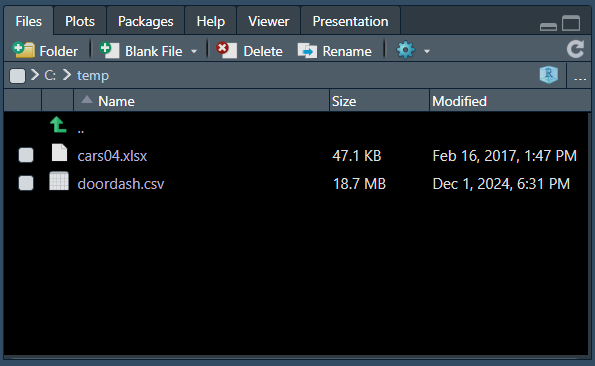
\includegraphics[width=5.4375in,height=\textheight,keepaspectratio]{images/utilitypane.png}

  }

  \caption{The \emph{Files} tab in the Utility Pane}

  \end{figure}%
\item
  Click on the file you want to import, and then choose \emph{Import
  Dataset\ldots{}}, which opens up an import wizard. We will be opening
  the \texttt{cars04.xlsx} file, which will ultimately requires us to
  use the \texttt{readxl} package (Wickham and Bryan 2023).

  \begin{figure}[H]

  {\centering 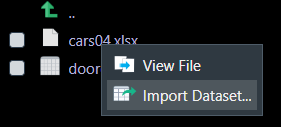
\includegraphics[width=2.35417in,height=\textheight,keepaspectratio]{images/import_dataset.png}

  }

  \caption{Choose \emph{Import Dataset\ldots{}}}

  \end{figure}%%
  \begin{figure}[H]

  {\centering \pandocbounded{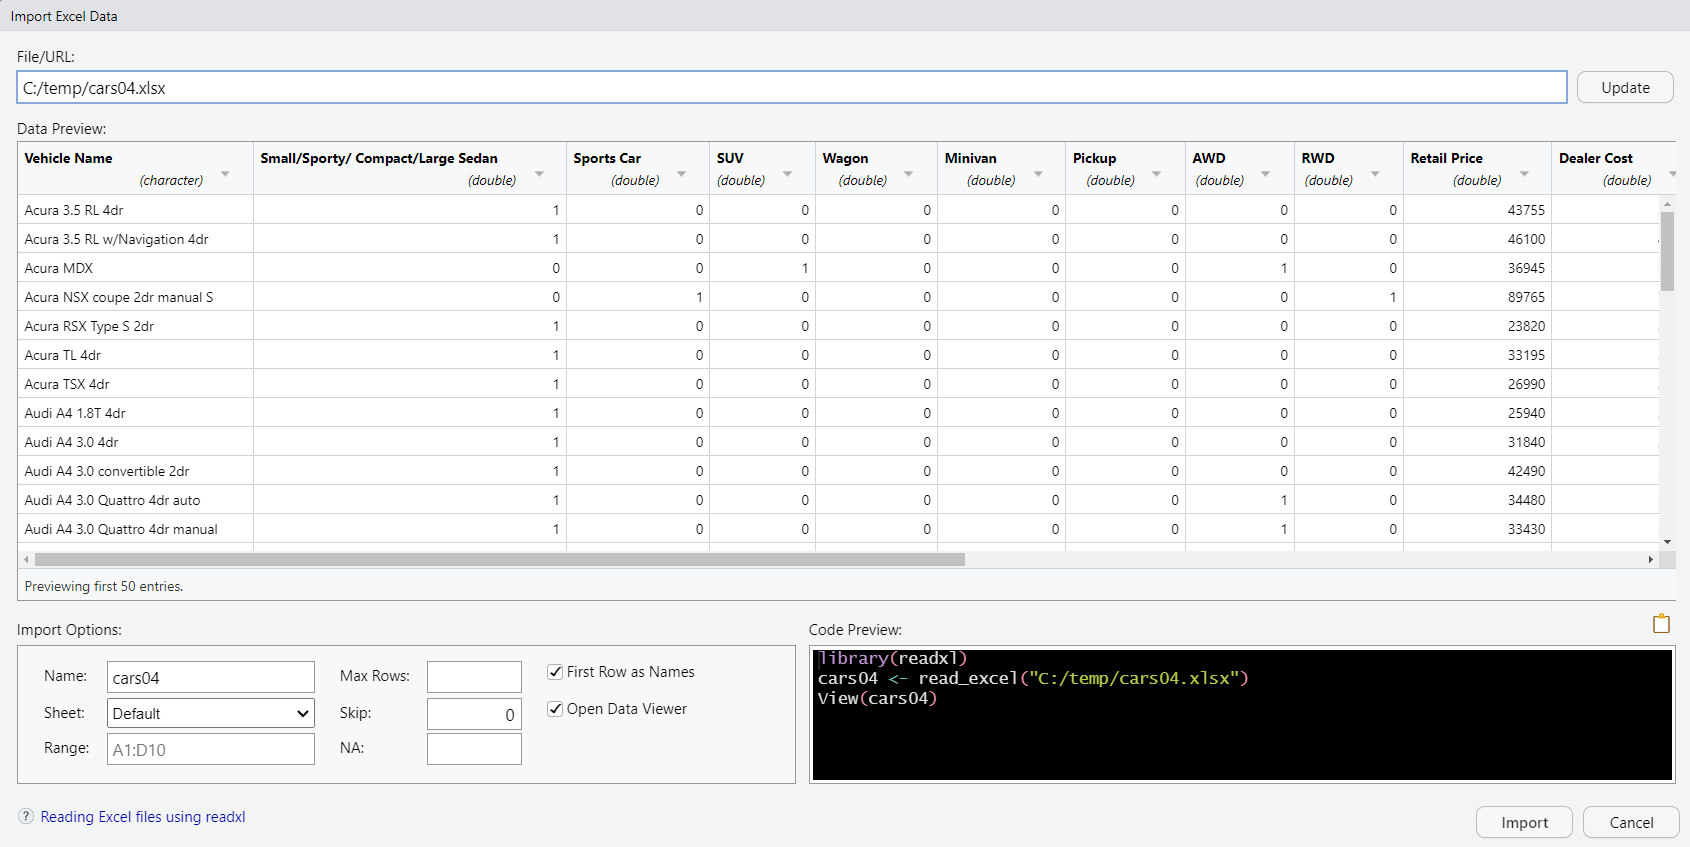
\includegraphics[keepaspectratio]{images/import_wizard.png}}

  }

  \caption{Excel Import Wizard}

  \end{figure}%
\item
  The import wizard should show you a preview of the first 50 rows of
  data. Make sure that it looks like the data should import correctly.
  Check your column names and variable types, especially if you skipped
  step 1 above. Here, I can see that I have my work cut out for me when
  it comes to variable names-the naming conventions are gross, there are
  spaces and characters I want to avoid (the variable named
  \texttt{Small/Sporty/\ Compact/Large\ Sedan} hurts my soul). As this
  is a small data set, I might want to open it up in excel first, rename
  everything there, and then redo the import. Or, I just anticipate
  doing this work with code. Regardless, at this point you want to
  evaluate whether or not you want to do the import right now, or if you
  want to clean up the file more before you import it. Let's assume that
  I want to just import the data now. The bottom right area of the
  import wizard has a section called \emph{Code Preview} with the code
  that will import the data. Clicking the import button will start the
  process, but you should also copy and paste this code into your script
  so you can use it later. Note that if you follow my advice from
  @sec-basicR R and Rstudio, you might want to actually put the
  \texttt{library()} calls at the beginning of your script. The third
  line, \texttt{View(cars04)}, just opens the newly created object in
  your viewer and you should probably toggle it off via the checkbox in
  the Import Options.
\end{enumerate}

And voilà, you're done! While these steps outline a general workflow for
importing data into R, the specifics can vary depending on the file
type, the structure of your data, and the packages you use. If you're
not diligent about using RStudio Projects and working directories, the
process can become trickier-you might need to include full file paths in
your import code, which can be cumbersome and error-prone, especially
when sharing your scripts with others or working on network drives.

While importing data from files is the most common method in the real
world, this book will primarily use datasets included in various R
packages. This approach ensures that you, dear reader, can access the
exact same data used in the examples without any hassle. And, as luck
would have it, it just so turns out that there is a slightly different
(and thankfully pre-formatted!) version of the \texttt{cars04} data in
the \texttt{openintro} package (Çetinkaya-Rundel et al. 2024)! Accessing
this data is as simple as loading the library:

\begin{Shaded}
\begin{Highlighting}[]
\FunctionTok{library}\NormalTok{(openintro) }
\end{Highlighting}
\end{Shaded}

And then loading the data into memory as an object with a single
command:

\begin{Shaded}
\begin{Highlighting}[]
\FunctionTok{data}\NormalTok{(cars04)}
\end{Highlighting}
\end{Shaded}

Simply executing the command \texttt{data(cars04)} creates an object
called \texttt{cars04} in your workspace. If you would prefer to give
the dataset a different name than its default, you can do so with the
assignment operator after the \texttt{openintro} library has been
loaded.

\begin{Shaded}
\begin{Highlighting}[]
\NormalTok{cars2004 }\OtherTok{\textless{}{-}}\NormalTok{ cars04}
\end{Highlighting}
\end{Shaded}

Typically, datasets loaded in this way will have a data dictionary that
you can check out with the help command. Either \texttt{?cars04} or
\texttt{help(cars04)} will open a help file in the Utility Pane, and you
can scroll through the file there to see more about what is in the
dataset. A couple important notes on this feature:

\begin{itemize}
\tightlist
\item
  You have to use the original dataset name, not something you assigned
  to it! For instance, in the above code chunk, we made an object called
  \texttt{cars2004} from the \texttt{cars04} data. However,
  \texttt{?cars2004} won't work!
\item
  The quality of these help files can vary-some are more useful and
  descriptive than others!
\end{itemize}

\section{Data Wrangling}\label{data-wrangling}

The term ``data wrangling'' refers to the process of cleaning,
organizing, combining, and transforming raw data into a format that will
make it easier to analyze and interpret. This typically involves tasks
like fixing errors, reformatting variables, creating and deleting
variables, and reorganizing data through sorting, grouping, and
filtering. How we wrangle the data is informed by the types of questions
we wish to answer; thus, it is an essential first step in data analysis,
because we need ensure that the data is appropriately structured to
support our goals.

The \texttt{dplyr} (Wickham et al. 2023) package in the
\texttt{tidyverse} (Wickham et al. 2019) houses most of the primary data
wrangling functions. The six most important \texttt{dplyr} verbs to
remember are:

\begin{itemize}
\tightlist
\item
  \texttt{select()} - Selects columns
\item
  \texttt{filter()} - Filters rows
\item
  \texttt{arrange()} - Re-orders rows
\item
  \texttt{mutate()} - Creates new columns
\item
  \texttt{summarize()} - summarizes variables
\item
  \texttt{group\_by()} - allows you to split-apply-recombine data along
  with \texttt{ungroup()}
\end{itemize}

Ok, I cheated a bit and snuck a 7th one in there. This section will
cover each of these verbs, and I'll certainly be throwing in a few more
along the way that I like to use (\texttt{distinct()}, \texttt{\%in\%},
\texttt{drop\_na()}, \texttt{n()}, \texttt{case\_when()}, and
\texttt{if\_else()} come immediately to mind). This section will by no
means be a comprehensive review of the \texttt{dplyr} or the
\texttt{tidyverse} and how they can be used; it should, however, provide
a solid foundation upon which to build. For a deeper dive in the
\texttt{tidyverse} family of packages, a good next step would be to
check out the free book \href{https://r4ds.hadley.nz/}{\emph{R for Data
Science}} (Wickham and Grolemund 2017).

On their own, each verb is not that powerful. But when combined with
others, they become mighty-kind of like the Infinity Gauntlet, the
Deathly Hallows and/or the Care Bear Stare. As a result, this section
will start with simple examples and quickly build to more complex,
powerful operations.

\subsection{The Pipe Operator}\label{the-pipe-operator}

Before we can dig too deeply into these verbs, we need to learn about
the pipe operator, \texttt{\textbar{}\textgreater{}}. The keyboard
shortcut in RStudio for the pipe is Ctrl + Shift + M (if this shortcut
produces \texttt{\%\textgreater{}\%} instead, go to \textbf{Tools
\(\rightarrow\) Global Options \(\rightarrow\) Code} and ensure that
``Use Native Pipe Operator'' is toggled on); this shortcut is worth
memorizing, as you will use it a lot!

We use pipes to pass the results from one line into the next line, which
creates a logical, step-by-step workflow. Typically, any data wrangling
we do is going to begin with something like this:

\begin{Shaded}
\begin{Highlighting}[]
\NormalTok{cars04 }\SpecialCharTok{|\textgreater{}} 
  \CommentTok{\# Data Wrangling!}
\end{Highlighting}
\end{Shaded}

This is telling R that I want to start with the \texttt{cars04} dataset
and put it into whatever I'm doing on the next line. Note that this does
not permanently change what is in \texttt{cars04}; it starts with
\texttt{cars04}, pipes it into whatever comes next where I put the
\texttt{\#\ Data\ Wrangling!} placeholder, but that's it. It doesn't
save it anywhere. In general, when we are data wrangling, we want to
retain the changes we made to the dataset, so we need to pair this with
the assignment operator.

\begin{Shaded}
\begin{Highlighting}[]
\NormalTok{cars\_data }\OtherTok{\textless{}{-}}\NormalTok{ cars04 }\SpecialCharTok{|\textgreater{}} 
  \CommentTok{\# Data Wrangling!}
\end{Highlighting}
\end{Shaded}

This workflow tells R to create a new dataset called \texttt{cars\_data}
that will store the result of my data wrangling that follows.

Another common option is to overwrite \texttt{cars04} with our wrangled
data:

\begin{Shaded}
\begin{Highlighting}[]
\NormalTok{cars04 }\OtherTok{\textless{}{-}}\NormalTok{ cars04 }\SpecialCharTok{|\textgreater{}} 
  \CommentTok{\# Data Wrangling! }
\end{Highlighting}
\end{Shaded}

This is fine, but keep in mind that once you have wrangled, you can't
always unwrangle. So if whatever follows this line of code doesn't work
right, you will have to redo everything up to this point, including
reloading in the data and any intermediate steps taken before you got to
this stage in your work. To avoid losing your original data, always
consider creating a new object for the transformed data.

\begin{tcolorbox}[enhanced jigsaw, colframe=quarto-callout-tip-color-frame, breakable, arc=.35mm, bottomtitle=1mm, bottomrule=.15mm, colbacktitle=quarto-callout-tip-color!10!white, rightrule=.15mm, colback=white, opacityback=0, opacitybacktitle=0.6, coltitle=black, left=2mm, toptitle=1mm, toprule=.15mm, titlerule=0mm, leftrule=.75mm, title=\textcolor{quarto-callout-tip-color}{\faLightbulb}\hspace{0.5em}{Tip from the Helpdesk: A Tale of Two Pipes}]

There are technically \emph{two} pipe operators that are commonly used
in R, \texttt{\textbar{}\textgreater{}} and \texttt{\%\textgreater{}\%}.
The first one, \texttt{\textbar{}\textgreater{}}, is part of Base R,
whereas the second one, \texttt{\%\textgreater{}\%}, is part of the
\texttt{magrittr} package in \texttt{tidyverse}. I will be using the
Base R version, but both do the same thing; pass the output of one line
into the next line.

If you are searching for R help on the internet, it is highly likely
that you will see a lot of people using the \texttt{\%\textgreater{}\%}
version. This is because the \texttt{\textbar{}\textgreater{}} version
was only added to Base R in 2021, whereas the
\texttt{\%\textgreater{}\%} pipe in the tidyverse has been around a lot
longer. If you see a \texttt{\%\textgreater{}\%}, just treat it like
\texttt{\textbar{}\textgreater{}}.

However, a word of caution: \texttt{\%\textgreater{}\%} requires loading
the \texttt{tidyverse.} If you use code with \texttt{\%\textgreater{}\%}
without first running \texttt{library(tidyverse)}, you'll encounter an
error like
\texttt{Error:\ could\ not\ find\ function\ "\%\textgreater{}\%"}. To
avoid this, either replace \texttt{\%\textgreater{}\%} with
\texttt{\textbar{}\textgreater{}} or make sure to load the
\texttt{tidyverse} first.

\end{tcolorbox}

Pipes can be, and are quite often, chained. I will explain more about
the commands in this next chunk when I get to the relevant sections
later in this chapter, but to illustrate the concept of chaining pipes,
let's say I want a list of the cars and prices in \texttt{cars04} that
had an MSRP (manufacturer's suggested retail price) over \$75,000, and I
want them in order from most to least expensive. This means I want to
get rid of all observations that don't match my criteria
(\texttt{filter}), get rid of all the other data about these cars
(\texttt{select}, and put them in order (\texttt{arrange}). I will do
these commands in order, piping the results of one command into the next
line:

\begin{Shaded}
\begin{Highlighting}[]
\NormalTok{cars04 }\SpecialCharTok{|\textgreater{}} 
  \FunctionTok{filter}\NormalTok{(msrp }\SpecialCharTok{\textgreater{}} \DecValTok{75000}\NormalTok{) }\SpecialCharTok{|\textgreater{}} 
  \FunctionTok{select}\NormalTok{(name, msrp) }\SpecialCharTok{|\textgreater{}} 
  \FunctionTok{arrange}\NormalTok{(}\SpecialCharTok{{-}}\NormalTok{msrp)}
\end{Highlighting}
\end{Shaded}

\begin{verbatim}
# A tibble: 17 x 2
   name                                          msrp
   <chr>                                        <int>
 1 Porsche 911 GT2 2dr                         192465
 2 Mercedes-Benz CL600 2dr                     128420
 3 Mercedes-Benz SL600 convertible 2dr         126670
 4 Mercedes-Benz SL55 AMG 2dr                  121770
 5 Mercedes-Benz CL500 2dr                      94820
 6 Mercedes-Benz SL500 convertible 2dr          90520
 7 Acura NSX coupe 2dr manual S                 89765
 8 Jaguar XKR convertible 2dr                   86995
 9 Mercedes-Benz S500 4dr                       86970
10 Audi RS 6 4dr                                84600
11 Porsche 911 Carrera 4S coupe 2dr (convert)   84165
12 Jaguar XKR coupe 2dr                         81995
13 Dodge Viper SRT-10 convertible 2dr           81795
14 Porsche 911 Carrera convertible 2dr (coupe)  79165
15 Mercedes-Benz G500                           76870
16 Porsche 911 Targa coupe 2dr                  76765
17 Cadillac XLR convertible 2dr                 76200
\end{verbatim}

When looking at code like this, the best way to read the
\texttt{\textbar{}\textgreater{}} is to say the words ``and then'' in
your mind when you are deciphering the code. In other words, the code
above says to take the \texttt{cars04} dataset, \emph{and then} filter
it, \emph{and then} select columns, \emph{and then} arrange the data
based on the \texttt{msrp} variable.

\begin{tcolorbox}[enhanced jigsaw, colframe=quarto-callout-tip-color-frame, breakable, arc=.35mm, bottomtitle=1mm, bottomrule=.15mm, colbacktitle=quarto-callout-tip-color!10!white, rightrule=.15mm, colback=white, opacityback=0, opacitybacktitle=0.6, coltitle=black, left=2mm, toptitle=1mm, toprule=.15mm, titlerule=0mm, leftrule=.75mm, title=\textcolor{quarto-callout-tip-color}{\faLightbulb}\hspace{0.5em}{Tip from the Helpdesk: One Line, One Thing}]

While it's not always possible, in general, you want each line of code
to do one thing and exactly one thing. Sure, breaking it up over several
lines as I did in the main text makes your code look longer. But,
breaking your code in to clear, single-task steps makes it easier to
read, debug, and understand. For example, that last code chunk
\emph{could} have been written like this, and it would work just fine:

\begin{Shaded}
\begin{Highlighting}[]
\NormalTok{cars04 }\SpecialCharTok{|\textgreater{}} \FunctionTok{filter}\NormalTok{(msrp }\SpecialCharTok{\textgreater{}} \DecValTok{75000}\NormalTok{) }\SpecialCharTok{|\textgreater{}} \FunctionTok{select}\NormalTok{(name, msrp) }\SpecialCharTok{|\textgreater{}} \FunctionTok{arrange}\NormalTok{(}\SpecialCharTok{{-}}\NormalTok{msrp)}
\end{Highlighting}
\end{Shaded}

While it would work, in general, you should strive to make your code
readable. Keeping the mantra of ``one line, one thing'' and having each
line of code accomplish one task goes a long way toward making your code
cleaner and your life easier.

\end{tcolorbox}

\subsection{Select}\label{select}

The \texttt{select()} function is pretty straightforward. It used to
select columns-typically, it is used to focus on or remove columns from
our data. There are a number of reasons we may want to do this, for
example:

\begin{itemize}
\item
  Simplifying visualizations: Maybe we are creating a table for a
  presentation, and while the dataset has 40 variables, we only want to
  include 3 or 4 of the variables in our chart.
\item
  Sensitive information: There may be personally identifiable
  information (PII) in a dataset, so if we want to share the data, we
  need to remove the PII first.
\item
  Huge datasets: If we have a huge dataset, working with it can be
  cumbersome for a computer. Eliminating variables we don't need will
  free up memory. Similarly, email systems may not be able to cope with
  huge datasets, and online cloud storage is not unlimited, so having
  streamlined data can be useful.
\end{itemize}

The two primary ways \texttt{select()} is used is to either, a) choose a
specific subset of variables, or b) to choose \emph{all but} a specific
subset of variables. To see both of these in action, let's load up the
\texttt{gapminder} data from the \texttt{gapminder} package and check
out the first few rows of data.

\begin{Shaded}
\begin{Highlighting}[]
\FunctionTok{data}\NormalTok{(gapminder)}
\FunctionTok{head}\NormalTok{(gapminder)}
\end{Highlighting}
\end{Shaded}

\begin{verbatim}
# A tibble: 6 x 6
  country     continent  year lifeExp      pop gdpPercap
  <fct>       <fct>     <int>   <dbl>    <int>     <dbl>
1 Afghanistan Asia       1952    28.8  8425333      779.
2 Afghanistan Asia       1957    30.3  9240934      821.
3 Afghanistan Asia       1962    32.0 10267083      853.
4 Afghanistan Asia       1967    34.0 11537966      836.
5 Afghanistan Asia       1972    36.1 13079460      740.
6 Afghanistan Asia       1977    38.4 14880372      786.
\end{verbatim}

For the first example, let's select only the \texttt{country},
\texttt{year}, and \texttt{gdpPercap} variables:

\begin{Shaded}
\begin{Highlighting}[]
\NormalTok{gapminder }\SpecialCharTok{|\textgreater{}} 
  \FunctionTok{select}\NormalTok{(country, year, gdpPercap) }\SpecialCharTok{|\textgreater{}} 
  \FunctionTok{head}\NormalTok{()}
\end{Highlighting}
\end{Shaded}

\begin{verbatim}
# A tibble: 6 x 3
  country      year gdpPercap
  <fct>       <int>     <dbl>
1 Afghanistan  1952      779.
2 Afghanistan  1957      821.
3 Afghanistan  1962      853.
4 Afghanistan  1967      836.
5 Afghanistan  1972      740.
6 Afghanistan  1977      786.
\end{verbatim}

Alternately, we can use the \texttt{select()} command to choose
everything \emph{but} one or more variables. For this functionality, put
a \texttt{-} sign before any variables you want to get rid of in your
data. Let's get rid of the \texttt{continent} and \texttt{pop}
variables.

\begin{Shaded}
\begin{Highlighting}[]
\NormalTok{gapminder }\SpecialCharTok{|\textgreater{}} 
  \FunctionTok{select}\NormalTok{(}\SpecialCharTok{{-}}\NormalTok{continent,}
         \SpecialCharTok{{-}}\NormalTok{pop) }\SpecialCharTok{|\textgreater{}} 
  \FunctionTok{head}\NormalTok{()}
\end{Highlighting}
\end{Shaded}

\begin{verbatim}
# A tibble: 6 x 4
  country      year lifeExp gdpPercap
  <fct>       <int>   <dbl>     <dbl>
1 Afghanistan  1952    28.8      779.
2 Afghanistan  1957    30.3      821.
3 Afghanistan  1962    32.0      853.
4 Afghanistan  1967    34.0      836.
5 Afghanistan  1972    36.1      740.
6 Afghanistan  1977    38.4      786.
\end{verbatim}

\begin{tcolorbox}[enhanced jigsaw, colframe=quarto-callout-tip-color-frame, breakable, arc=.35mm, bottomtitle=1mm, bottomrule=.15mm, colbacktitle=quarto-callout-tip-color!10!white, rightrule=.15mm, colback=white, opacityback=0, opacitybacktitle=0.6, coltitle=black, left=2mm, toptitle=1mm, toprule=.15mm, titlerule=0mm, leftrule=.75mm, title=\textcolor{quarto-callout-tip-color}{\faLightbulb}\hspace{0.5em}{Tip from the Helpdesk: One Line, One Thing, Strikes Again}]

You may have noticed a subtle difference between the two preceding sets
of code: the second one follows the \emph{One Line, One Thing} rule more
closely by placing each variable in the \texttt{select()} command on its
own line.

At first glance, this may seem like overkill. But trust me, as we get
into more complicated coding, this syntax will make your code much
easier to read, debug, and modify!

\end{tcolorbox}

In short, \texttt{select()} provides a simple and straightforward way to
tailor your dataset to include or exclude specific variables. We will
continue to make use of \texttt{select()} as we move through the list of
essential \texttt{dplyr} verbs.

\subsection{Filter}\label{filter}

Whereas \texttt{select()} helps us choose which columns we wanted to
have in our dataset, \texttt{filter()} is like a sieve for the rows in
our dataset-it allows us to keep only the rows that meet specific
conditions. Filtering is generally a bit more complex than selecting,
because it typically involves the use of logical conditions.

\subsubsection{Basic Comparitors}\label{basic-comparitors}

The most basic comparitors are the ones you will get the most use out
of: \texttt{\textgreater{}},\texttt{\textless{}},
\texttt{\textgreater{}=},\texttt{\textless{}=}, \texttt{!=}, and
\texttt{==}. Don't forget, for equals we use \texttt{==} instead of
\texttt{=}!

Let's use a couple of these. First, let's filter the \texttt{gapminder}
dataset to only include data from 1977:

\begin{Shaded}
\begin{Highlighting}[]
\NormalTok{gapminder }\SpecialCharTok{|\textgreater{}} 
  \FunctionTok{filter}\NormalTok{(year }\SpecialCharTok{==} \DecValTok{1977}\NormalTok{) }
\end{Highlighting}
\end{Shaded}

\begin{verbatim}
# A tibble: 142 x 6
   country     continent  year lifeExp      pop gdpPercap
   <fct>       <fct>     <int>   <dbl>    <int>     <dbl>
 1 Afghanistan Asia       1977    38.4 14880372      786.
 2 Albania     Europe     1977    68.9  2509048     3533.
 3 Algeria     Africa     1977    58.0 17152804     4910.
 4 Angola      Africa     1977    39.5  6162675     3009.
 5 Argentina   Americas   1977    68.5 26983828    10079.
 6 Australia   Oceania    1977    73.5 14074100    18334.
 7 Austria     Europe     1977    72.2  7568430    19749.
 8 Bahrain     Asia       1977    65.6   297410    19340.
 9 Bangladesh  Asia       1977    46.9 80428306      660.
10 Belgium     Europe     1977    72.8  9821800    19118.
# i 132 more rows
\end{verbatim}

Note that if we had written \texttt{filter(year\ =\ 1977)}, the code
wouldn't have worked. We would have received an error that says
something like: ``Error in filter(gapminder, year = 1977) : unused
argument (year = 1977).''

Let's use filter to see every country with \texttt{gdpPercap} less than
or equal to 300.

\begin{Shaded}
\begin{Highlighting}[]
\NormalTok{gapminder }\SpecialCharTok{|\textgreater{}} 
  \FunctionTok{filter}\NormalTok{(gdpPercap }\SpecialCharTok{\textless{}=} \DecValTok{300}\NormalTok{)}
\end{Highlighting}
\end{Shaded}

\begin{verbatim}
# A tibble: 4 x 6
  country          continent  year lifeExp      pop gdpPercap
  <fct>            <fct>     <int>   <dbl>    <int>     <dbl>
1 Congo, Dem. Rep. Africa     2002    45.0 55379852      241.
2 Congo, Dem. Rep. Africa     2007    46.5 64606759      278.
3 Guinea-Bissau    Africa     1952    32.5   580653      300.
4 Lesotho          Africa     1952    42.1   748747      299.
\end{verbatim}

\subsubsection{Factor and Character
Variables}\label{factor-and-character-variables}

When applying a condition to a character variable, you need to wrap the
condition in quotation marks.

For example, let's filter the data to only include Canada:

\begin{Shaded}
\begin{Highlighting}[]
\NormalTok{gapminder }\SpecialCharTok{|\textgreater{}} 
  \FunctionTok{filter}\NormalTok{(country }\SpecialCharTok{==} \StringTok{"Canada"}\NormalTok{)}
\end{Highlighting}
\end{Shaded}

\begin{verbatim}
# A tibble: 12 x 6
   country continent  year lifeExp      pop gdpPercap
   <fct>   <fct>     <int>   <dbl>    <int>     <dbl>
 1 Canada  Americas   1952    68.8 14785584    11367.
 2 Canada  Americas   1957    70.0 17010154    12490.
 3 Canada  Americas   1962    71.3 18985849    13462.
 4 Canada  Americas   1967    72.1 20819767    16077.
 5 Canada  Americas   1972    72.9 22284500    18971.
 6 Canada  Americas   1977    74.2 23796400    22091.
 7 Canada  Americas   1982    75.8 25201900    22899.
 8 Canada  Americas   1987    76.9 26549700    26627.
 9 Canada  Americas   1992    78.0 28523502    26343.
10 Canada  Americas   1997    78.6 30305843    28955.
11 Canada  Americas   2002    79.8 31902268    33329.
12 Canada  Americas   2007    80.7 33390141    36319.
\end{verbatim}

Had we forgotten the quotation marks and entered
\texttt{filter(country\ ==\ Canada)}, R would throw an error.

Or, perhaps we want to get rid of Canada from our dataset?

\begin{Shaded}
\begin{Highlighting}[]
\NormalTok{gapminder }\SpecialCharTok{|\textgreater{}} 
  \FunctionTok{filter}\NormalTok{(country }\SpecialCharTok{!=} \StringTok{"Canada"}\NormalTok{)}
\end{Highlighting}
\end{Shaded}

\begin{verbatim}
# A tibble: 1,692 x 6
   country     continent  year lifeExp      pop gdpPercap
   <fct>       <fct>     <int>   <dbl>    <int>     <dbl>
 1 Afghanistan Asia       1952    28.8  8425333      779.
 2 Afghanistan Asia       1957    30.3  9240934      821.
 3 Afghanistan Asia       1962    32.0 10267083      853.
 4 Afghanistan Asia       1967    34.0 11537966      836.
 5 Afghanistan Asia       1972    36.1 13079460      740.
 6 Afghanistan Asia       1977    38.4 14880372      786.
 7 Afghanistan Asia       1982    39.9 12881816      978.
 8 Afghanistan Asia       1987    40.8 13867957      852.
 9 Afghanistan Asia       1992    41.7 16317921      649.
10 Afghanistan Asia       1997    41.8 22227415      635.
# i 1,682 more rows
\end{verbatim}

Remember, spelling and capitalization count and R is super strict about
it. For instance, the \texttt{gapminder} dataset codes North Korea as
\texttt{Korea,\ Dem.\ Rep.}. If we want to filter the data for North
Korea, \texttt{filter(country\ ==\ "Korea,\ Dem.\ Rep.")} works, but
none of the following would as they don't \textbf{exactly} match:

\begin{itemize}
\tightlist
\item
  \texttt{filter(country\ ==\ "Korea,\ Dem\ Rep")}
\item
  \texttt{filter(country\ ==\ "North\ Korea")}
\item
  \texttt{filter(country\ ==\ "N\ Korea")}
\item
  \texttt{filter(country\ ==\ "korea,\ dem.\ rep.")}
\item
  \texttt{filter(country\ ==\ "Democratic\ People\textquotesingle{}s\ Republic\ of\ Korea")}
\end{itemize}

When working with datasets, It is important to always check for the
exact formatting of character variables, as even small discrepancies can
cause your code to break in spectacular fashion.

\subsubsection{Multiple Filters}\label{multiple-filters}

You can include multiple filters in the same \texttt{filter()} command,
separated by commas. This is equivalent to a Boolean \textbf{AND}
condition, meaning that only rows that meet all the specified conditions
will be included in the result. Alternately, you can use a Boolean
\textbf{OR} in a filter with the \texttt{\textbar{}} operator. This
means that rows that match \emph{any} of the conditions will be included
in the result. Let's see how these work with some examples:

First, let's filter our data to only include European countries in 1952.
And since we only have European countries in our data, let's combine
this with a \texttt{select()} function; since we only have European
countries, the \texttt{continent} variable is kinda meaningless:

\begin{Shaded}
\begin{Highlighting}[]
\NormalTok{gapminder }\SpecialCharTok{|\textgreater{}} 
  \FunctionTok{filter}\NormalTok{(continent }\SpecialCharTok{==} \StringTok{"Europe"}\NormalTok{,}
\NormalTok{         year }\SpecialCharTok{==} \DecValTok{1952}\NormalTok{) }\SpecialCharTok{|\textgreater{}} 
  \FunctionTok{select}\NormalTok{(}\SpecialCharTok{{-}}\NormalTok{continent)}
\end{Highlighting}
\end{Shaded}

\begin{verbatim}
# A tibble: 30 x 5
   country                 year lifeExp      pop gdpPercap
   <fct>                  <int>   <dbl>    <int>     <dbl>
 1 Albania                 1952    55.2  1282697     1601.
 2 Austria                 1952    66.8  6927772     6137.
 3 Belgium                 1952    68    8730405     8343.
 4 Bosnia and Herzegovina  1952    53.8  2791000      974.
 5 Bulgaria                1952    59.6  7274900     2444.
 6 Croatia                 1952    61.2  3882229     3119.
 7 Czech Republic          1952    66.9  9125183     6876.
 8 Denmark                 1952    70.8  4334000     9692.
 9 Finland                 1952    66.6  4090500     6425.
10 France                  1952    67.4 42459667     7030.
# i 20 more rows
\end{verbatim}

Because the \texttt{filter()} command works sequentially, this is
equivalent to the following:

\begin{Shaded}
\begin{Highlighting}[]
\NormalTok{gapminder }\SpecialCharTok{|\textgreater{}} 
  \FunctionTok{filter}\NormalTok{(continent }\SpecialCharTok{==} \StringTok{"Europe"}\NormalTok{) }\SpecialCharTok{|\textgreater{}} 
  \FunctionTok{filter}\NormalTok{(year }\SpecialCharTok{==} \DecValTok{1952}\NormalTok{) }\SpecialCharTok{|\textgreater{}} 
  \FunctionTok{select}\NormalTok{(}\SpecialCharTok{{-}}\NormalTok{continent)}
\end{Highlighting}
\end{Shaded}

Either option is fine. For me, the more complex the filtering operation,
the more I tend to lean toward the second version. For example, working
with the Boolean \textbf{or} filter is a bit trickier. With an or, we
are going to filter not based on whether or not \textbf{all} of a set of
conditions are true, but rather based on if \textbf{any} of a set of
conditions are true. For these, you need to include all the
possibilities in the same filter argument, and separate the different
possible qualifying conditions with a \texttt{\textbar{}}. For example,
let's get wrangle our data to get 2007 data for countries in either
Oceania or Asia:

\begin{Shaded}
\begin{Highlighting}[]
\NormalTok{gapminder }\SpecialCharTok{|\textgreater{}} 
  \FunctionTok{filter}\NormalTok{(continent }\SpecialCharTok{==} \StringTok{"Asia"} \SpecialCharTok{|}\NormalTok{ continent}\SpecialCharTok{==} \StringTok{"Oceania"}\NormalTok{) }\SpecialCharTok{|\textgreater{}} 
  \FunctionTok{filter}\NormalTok{(year }\SpecialCharTok{==} \DecValTok{2007}\NormalTok{)}
\end{Highlighting}
\end{Shaded}

\begin{verbatim}
# A tibble: 35 x 6
   country          continent  year lifeExp        pop gdpPercap
   <fct>            <fct>     <int>   <dbl>      <int>     <dbl>
 1 Afghanistan      Asia       2007    43.8   31889923      975.
 2 Australia        Oceania    2007    81.2   20434176    34435.
 3 Bahrain          Asia       2007    75.6     708573    29796.
 4 Bangladesh       Asia       2007    64.1  150448339     1391.
 5 Cambodia         Asia       2007    59.7   14131858     1714.
 6 China            Asia       2007    73.0 1318683096     4959.
 7 Hong Kong, China Asia       2007    82.2    6980412    39725.
 8 India            Asia       2007    64.7 1110396331     2452.
 9 Indonesia        Asia       2007    70.6  223547000     3541.
10 Iran             Asia       2007    71.0   69453570    11606.
# i 25 more rows
\end{verbatim}

While the \texttt{\textbar{}} or is powerful, when you have a lot of
different possible allowable conditions, the syntax might get
cumbersome. For example, if I had a list of 6 countries I wanted to
collect in my data, that \texttt{filter()} line might get a bit ugly.
This is a good place to use a special comparator, the \texttt{\%in\%}.
Let's wrangle out the 1992 data for each of the 6 Central American
countries in the \texttt{gapminder} data (Belize is not in the dataset):

\begin{Shaded}
\begin{Highlighting}[]
\NormalTok{gapminder }\SpecialCharTok{|\textgreater{}} 
  \FunctionTok{filter}\NormalTok{(country }\SpecialCharTok{\%in\%} \FunctionTok{c}\NormalTok{(}\StringTok{"Costa Rica"}\NormalTok{, }
                        \StringTok{"El Salvador"}\NormalTok{, }
                        \StringTok{"Guatemala"}\NormalTok{, }
                        \StringTok{"Honduras"}\NormalTok{, }
                        \StringTok{"Nicaragua"}\NormalTok{, }
                        \StringTok{"Panama"}\NormalTok{)) }\SpecialCharTok{|\textgreater{}} 
  \FunctionTok{filter}\NormalTok{(year }\SpecialCharTok{==} \DecValTok{1992}\NormalTok{)}
\end{Highlighting}
\end{Shaded}

\begin{verbatim}
# A tibble: 6 x 6
  country     continent  year lifeExp     pop gdpPercap
  <fct>       <fct>     <int>   <dbl>   <int>     <dbl>
1 Costa Rica  Americas   1992    75.7 3173216     6160.
2 El Salvador Americas   1992    66.8 5274649     4444.
3 Guatemala   Americas   1992    63.4 8486949     4439.
4 Honduras    Americas   1992    66.4 5077347     3082.
5 Nicaragua   Americas   1992    65.8 4017939     2170.
6 Panama      Americas   1992    72.5 2484997     6619.
\end{verbatim}

In addition to being simpler, the \texttt{\%in\%} syntax is very useful
for combining with lists. For example, if I already have a list of
Central American countries in a list called \texttt{countries}, I can
simply use the \texttt{\%in\%} to refer to that list:

\begin{Shaded}
\begin{Highlighting}[]
\NormalTok{countries }\OtherTok{\textless{}{-}} \FunctionTok{c}\NormalTok{(}\StringTok{"Costa Rica"}\NormalTok{,}
               \StringTok{"El Salvador"}\NormalTok{,}
               \StringTok{"Guatemala"}\NormalTok{,}
               \StringTok{"Honduras"}\NormalTok{,}
               \StringTok{"Nicaragua"}\NormalTok{, }
               \StringTok{"Panama"}\NormalTok{)}
\NormalTok{gapminder }\SpecialCharTok{|\textgreater{}} 
  \FunctionTok{filter}\NormalTok{(country }\SpecialCharTok{\%in\%}\NormalTok{ countries, }
\NormalTok{         year }\SpecialCharTok{==} \DecValTok{1992}\NormalTok{)}
\end{Highlighting}
\end{Shaded}

\begin{verbatim}
# A tibble: 6 x 6
  country     continent  year lifeExp     pop gdpPercap
  <fct>       <fct>     <int>   <dbl>   <int>     <dbl>
1 Costa Rica  Americas   1992    75.7 3173216     6160.
2 El Salvador Americas   1992    66.8 5274649     4444.
3 Guatemala   Americas   1992    63.4 8486949     4439.
4 Honduras    Americas   1992    66.4 5077347     3082.
5 Nicaragua   Americas   1992    65.8 4017939     2170.
6 Panama      Americas   1992    72.5 2484997     6619.
\end{verbatim}

Finally, another valuable use of filtering is to remove rows with
missing values from your data. To see this in action, let's turn to the
\texttt{cars04} data and look at the results of \texttt{summary()} to
identify which variables have missing values.

\begin{Shaded}
\begin{Highlighting}[]
\FunctionTok{summary}\NormalTok{(cars04)}
\end{Highlighting}
\end{Shaded}

\begin{verbatim}
     name           sports_car         suv            wagon        
 Length:428         Mode :logical   Mode :logical   Mode :logical  
 Class :character   FALSE:379       FALSE:368       FALSE:398      
 Mode  :character   TRUE :49        TRUE :60        TRUE :30       
                                                                   
                                                                   
                                                                   
                                                                   
  minivan          pickup        all_wheel       rear_wheel     
 Mode :logical   Mode :logical   Mode :logical   Mode :logical  
 FALSE:408       FALSE:404       FALSE:336       FALSE:318      
 TRUE :20        TRUE :24        TRUE :92        TRUE :110      
                                                                
                                                                
                                                                
                                                                
      msrp         dealer_cost        eng_size          ncyl       
 Min.   : 10280   Min.   :  9875   Min.   :1.300   Min.   :-1.000  
 1st Qu.: 20334   1st Qu.: 18866   1st Qu.:2.375   1st Qu.: 4.000  
 Median : 27635   Median : 25295   Median :3.000   Median : 6.000  
 Mean   : 32775   Mean   : 30015   Mean   :3.197   Mean   : 5.776  
 3rd Qu.: 39205   3rd Qu.: 35710   3rd Qu.:3.900   3rd Qu.: 6.000  
 Max.   :192465   Max.   :173560   Max.   :8.300   Max.   :12.000  
                                                                   
    horsepwr        city_mpg        hwy_mpg          weight       wheel_base   
 Min.   : 73.0   Min.   :10.00   Min.   :12.00   Min.   :1850   Min.   : 89.0  
 1st Qu.:165.0   1st Qu.:17.00   1st Qu.:24.00   1st Qu.:3102   1st Qu.:103.0  
 Median :210.0   Median :19.00   Median :26.00   Median :3474   Median :107.0  
 Mean   :215.9   Mean   :20.09   Mean   :26.91   Mean   :3577   Mean   :108.2  
 3rd Qu.:255.0   3rd Qu.:21.00   3rd Qu.:29.00   3rd Qu.:3974   3rd Qu.:112.0  
 Max.   :500.0   Max.   :60.00   Max.   :66.00   Max.   :7190   Max.   :144.0  
                 NA's   :14      NA's   :14      NA's   :2      NA's   :2      
     length          width      
 Min.   :143.0   Min.   :64.00  
 1st Qu.:177.0   1st Qu.:69.00  
 Median :186.0   Median :71.00  
 Mean   :185.1   Mean   :71.29  
 3rd Qu.:193.0   3rd Qu.:73.00  
 Max.   :227.0   Max.   :81.00  
 NA's   :26      NA's   :28     
\end{verbatim}

It seems that there are some missing values
(\texttt{NA\textquotesingle{}s}) for a few of the variables:
\texttt{city\_mpg}, \texttt{hwy\_mpg}, \texttt{weight},
\texttt{wheel\_base}, \texttt{length}, and \texttt{width}. Missing
values can cause errors, so we might want to explore ways to get rid of
them. When dealing missing values, \texttt{is.na()}, \texttt{!is.na()},
and \texttt{drop\_na()} come in handy. Let's focus on the
\texttt{hwy\_mpg} variable.

We can use \texttt{is.na()} to see which rows have a missing value. For
example, to see which cars we don't have data on highway MPG for, we
type:

\begin{Shaded}
\begin{Highlighting}[]
\NormalTok{cars04 }\SpecialCharTok{|\textgreater{}} 
  \FunctionTok{select}\NormalTok{(name, hwy\_mpg) }\SpecialCharTok{|\textgreater{}} 
  \FunctionTok{filter}\NormalTok{(}\FunctionTok{is.na}\NormalTok{(hwy\_mpg))}
\end{Highlighting}
\end{Shaded}

\begin{verbatim}
# A tibble: 14 x 2
   name                                hwy_mpg
   <chr>                                 <int>
 1 Mazda3 i 4dr                             NA
 2 Mitsubishi Lancer ES 4dr                 NA
 3 Mitsubishi Lancer LS 4dr                 NA
 4 Mazda3 s 4dr                             NA
 5 Mitsubishi Galant ES 2.4L 4dr            NA
 6 Mitsubishi Lancer OZ Rally 4dr auto      NA
 7 Pontiac Bonneville GXP 4dr               NA
 8 Volkswagen Phaeton 4dr                   NA
 9 Volkswagen Phaeton W12 4dr               NA
10 Dodge Viper SRT-10 convertible 2dr       NA
11 Pontiac GTO 2dr                          NA
12 Ford Excursion 6.8 XLT                   NA
13 Mitsubishi Lancer Sportback LS           NA
14 GMC Sierra HD 2500                       NA
\end{verbatim}

This shows rows where \texttt{hwy\_mpg} is missing.

If we wanted to analyze the highway MPG variable, keeping these
observation in the dataset is not very helpful, and in fact may cause R
to throw errors. This is where we might want to use \texttt{!is.na()},
which is the opposite of \texttt{is.na()}; it filters rows for which we
\emph{do} have data!

\begin{Shaded}
\begin{Highlighting}[]
\NormalTok{cars04 }\SpecialCharTok{|\textgreater{}} 
  \FunctionTok{filter}\NormalTok{(}\SpecialCharTok{!}\FunctionTok{is.na}\NormalTok{(hwy\_mpg))}
\end{Highlighting}
\end{Shaded}

\begin{verbatim}
# A tibble: 414 x 19
   name         sports_car suv   wagon minivan pickup all_wheel rear_wheel  msrp
   <chr>        <lgl>      <lgl> <lgl> <lgl>   <lgl>  <lgl>     <lgl>      <int>
 1 Chevrolet A~ FALSE      FALSE FALSE FALSE   FALSE  FALSE     FALSE      11690
 2 Chevrolet A~ FALSE      FALSE FALSE FALSE   FALSE  FALSE     FALSE      12585
 3 Chevrolet C~ FALSE      FALSE FALSE FALSE   FALSE  FALSE     FALSE      14610
 4 Chevrolet C~ FALSE      FALSE FALSE FALSE   FALSE  FALSE     FALSE      14810
 5 Chevrolet C~ FALSE      FALSE FALSE FALSE   FALSE  FALSE     FALSE      16385
 6 Dodge Neon ~ FALSE      FALSE FALSE FALSE   FALSE  FALSE     FALSE      13670
 7 Dodge Neon ~ FALSE      FALSE FALSE FALSE   FALSE  FALSE     FALSE      15040
 8 Ford Focus ~ FALSE      FALSE FALSE FALSE   FALSE  FALSE     FALSE      13270
 9 Ford Focus ~ FALSE      FALSE FALSE FALSE   FALSE  FALSE     FALSE      13730
10 Ford Focus ~ FALSE      FALSE FALSE FALSE   FALSE  FALSE     FALSE      15460
# i 404 more rows
# i 10 more variables: dealer_cost <int>, eng_size <dbl>, ncyl <int>,
#   horsepwr <int>, city_mpg <int>, hwy_mpg <int>, weight <int>,
#   wheel_base <int>, length <int>, width <int>
\end{verbatim}

Finally, \texttt{drop\_na()} is like an extreme version of filtering
with \texttt{!is.na()}. This is a \texttt{tidyverse} command that is
like a special version of \texttt{filter()} that drops any row that has
\emph{any} missing values.

\begin{Shaded}
\begin{Highlighting}[]
\NormalTok{cars04 }\SpecialCharTok{|\textgreater{}} 
  \FunctionTok{drop\_na}\NormalTok{()}
\end{Highlighting}
\end{Shaded}

\begin{verbatim}
# A tibble: 387 x 19
   name         sports_car suv   wagon minivan pickup all_wheel rear_wheel  msrp
   <chr>        <lgl>      <lgl> <lgl> <lgl>   <lgl>  <lgl>     <lgl>      <int>
 1 Chevrolet A~ FALSE      FALSE FALSE FALSE   FALSE  FALSE     FALSE      11690
 2 Chevrolet A~ FALSE      FALSE FALSE FALSE   FALSE  FALSE     FALSE      12585
 3 Chevrolet C~ FALSE      FALSE FALSE FALSE   FALSE  FALSE     FALSE      14610
 4 Chevrolet C~ FALSE      FALSE FALSE FALSE   FALSE  FALSE     FALSE      14810
 5 Chevrolet C~ FALSE      FALSE FALSE FALSE   FALSE  FALSE     FALSE      16385
 6 Dodge Neon ~ FALSE      FALSE FALSE FALSE   FALSE  FALSE     FALSE      13670
 7 Dodge Neon ~ FALSE      FALSE FALSE FALSE   FALSE  FALSE     FALSE      15040
 8 Ford Focus ~ FALSE      FALSE FALSE FALSE   FALSE  FALSE     FALSE      13270
 9 Ford Focus ~ FALSE      FALSE FALSE FALSE   FALSE  FALSE     FALSE      13730
10 Ford Focus ~ FALSE      FALSE FALSE FALSE   FALSE  FALSE     FALSE      15460
# i 377 more rows
# i 10 more variables: dealer_cost <int>, eng_size <dbl>, ncyl <int>,
#   horsepwr <int>, city_mpg <int>, hwy_mpg <int>, weight <int>,
#   wheel_base <int>, length <int>, width <int>
\end{verbatim}

\begin{tcolorbox}[enhanced jigsaw, colframe=quarto-callout-tip-color-frame, breakable, arc=.35mm, bottomtitle=1mm, bottomrule=.15mm, colbacktitle=quarto-callout-tip-color!10!white, rightrule=.15mm, colback=white, opacityback=0, opacitybacktitle=0.6, coltitle=black, left=2mm, toptitle=1mm, toprule=.15mm, titlerule=0mm, leftrule=.75mm, title=\textcolor{quarto-callout-tip-color}{\faLightbulb}\hspace{0.5em}{Tip from the Helpdesk: Cleaning with a Toothbrush or a Flamethrower?}]

Be careful with deciding between \texttt{filter(!is.na())} and
\texttt{drop\_na()}!

\begin{itemize}
\tightlist
\item
  \texttt{filter(!is.na())} is like cleaning with a toothbrush-precise
  and targeted but takes more effort.
\item
  \texttt{drop\_na()} is the flamethrower-quick and thorough but risks
  removing more rows than necessary.
\end{itemize}

Before you pick your weapon of choice, always explore your data to
understand where the missing values are and how much cleaning you
actually need! Especially with large datasets, \texttt{drop\_na()} can
be particularly aggressive, so double-check which columns contain
missing values before using it.

\end{tcolorbox}

\subsection{Arrange}\label{arrange}

The \texttt{arrange()} function allows us to sort a dataset by one or
more particular columns. Arranging is often useful when creating tables,
prepping data for visualization, or identifying extreme values.

The default behavior of \texttt{arrange()} is to sort numbers from
lowest to highest, or strings alphabetically. For example, we can see
the cars with the worst gas mileage:

\begin{Shaded}
\begin{Highlighting}[]
\NormalTok{cars04 }\SpecialCharTok{|\textgreater{}} 
  \FunctionTok{arrange}\NormalTok{(city\_mpg) }\SpecialCharTok{|\textgreater{}} 
  \FunctionTok{select}\NormalTok{(name, }
\NormalTok{         city\_mpg)}
\end{Highlighting}
\end{Shaded}

\begin{verbatim}
# A tibble: 428 x 2
   name                                city_mpg
   <chr>                                  <int>
 1 Hummer H2                                 10
 2 Land Rover Range Rover HSE                12
 3 Land Rover Discovery SE                   12
 4 Mercedes-Benz CL600 2dr                   13
 5 Mercedes-Benz SL600 convertible 2dr       13
 6 GMC Yukon XL 2500 SLT                     13
 7 Lincoln Navigator Luxury                  13
 8 Nissan Pathfinder Armada SE               13
 9 Lexus LX 470                              13
10 Lincoln Aviator Ultimate                  13
# i 418 more rows
\end{verbatim}

Or we can see the cars alphabetically:

\begin{Shaded}
\begin{Highlighting}[]
\NormalTok{cars04 }\SpecialCharTok{|\textgreater{}} 
  \FunctionTok{arrange}\NormalTok{(name) }
\end{Highlighting}
\end{Shaded}

\begin{verbatim}
# A tibble: 428 x 19
   name         sports_car suv   wagon minivan pickup all_wheel rear_wheel  msrp
   <chr>        <lgl>      <lgl> <lgl> <lgl>   <lgl>  <lgl>     <lgl>      <int>
 1 Acura 3.5 R~ FALSE      FALSE FALSE FALSE   FALSE  FALSE     FALSE      43755
 2 Acura 3.5 R~ FALSE      FALSE FALSE FALSE   FALSE  FALSE     FALSE      46100
 3 Acura MDX    FALSE      TRUE  FALSE FALSE   FALSE  TRUE      FALSE      36945
 4 Acura NSX c~ TRUE       FALSE FALSE FALSE   FALSE  FALSE     TRUE       89765
 5 Acura RSX T~ FALSE      FALSE FALSE FALSE   FALSE  FALSE     FALSE      23820
 6 Acura TL 4dr FALSE      FALSE FALSE FALSE   FALSE  FALSE     FALSE      33195
 7 Acura TSX 4~ FALSE      FALSE FALSE FALSE   FALSE  FALSE     FALSE      26990
 8 Audi A4 1.8~ FALSE      FALSE FALSE FALSE   FALSE  FALSE     FALSE      25940
 9 Audi A4 3.0~ FALSE      FALSE FALSE FALSE   FALSE  FALSE     FALSE      31840
10 Audi A4 3.0~ FALSE      FALSE FALSE FALSE   FALSE  TRUE      FALSE      34480
# i 418 more rows
# i 10 more variables: dealer_cost <int>, eng_size <dbl>, ncyl <int>,
#   horsepwr <int>, city_mpg <int>, hwy_mpg <int>, weight <int>,
#   wheel_base <int>, length <int>, width <int>
\end{verbatim}

We can reverse the order with a \texttt{-} sign in front of the sorted
variable. Here are the 10 most powerful cars in 2004:

\begin{Shaded}
\begin{Highlighting}[]
\NormalTok{cars04 }\SpecialCharTok{|\textgreater{}} 
  \FunctionTok{arrange}\NormalTok{(}\SpecialCharTok{{-}}\NormalTok{horsepwr) }\SpecialCharTok{|\textgreater{}} 
  \FunctionTok{select}\NormalTok{(name, }
\NormalTok{         horsepwr) }\SpecialCharTok{|\textgreater{}} 
  \FunctionTok{slice}\NormalTok{(}\DecValTok{1}\SpecialCharTok{:}\DecValTok{10}\NormalTok{)}
\end{Highlighting}
\end{Shaded}

\begin{verbatim}
# A tibble: 10 x 2
   name                                horsepwr
   <chr>                                  <int>
 1 Dodge Viper SRT-10 convertible 2dr       500
 2 Mercedes-Benz CL600 2dr                  493
 3 Mercedes-Benz SL55 AMG 2dr               493
 4 Mercedes-Benz SL600 convertible 2dr      493
 5 Porsche 911 GT2 2dr                      477
 6 Audi RS 6 4dr                            450
 7 Volkswagen Phaeton W12 4dr               420
 8 Jaguar S-Type R 4dr                      390
 9 Jaguar XJR 4dr                           390
10 Jaguar XKR coupe 2dr                     390
\end{verbatim}

The \texttt{slice(1:10)} line tells R to just show us the first 10 lines
of data.

If we specify multiple variables for the \texttt{arrange()}, it will
sort by the first variable first, and then ``break ties'' with the
subsequent variables. Here, we arrange by both engine size and
horsepower:

\begin{Shaded}
\begin{Highlighting}[]
\NormalTok{cars04 }\SpecialCharTok{|\textgreater{}} 
  \FunctionTok{arrange}\NormalTok{(}\SpecialCharTok{{-}}\NormalTok{eng\_size, }
          \SpecialCharTok{{-}}\NormalTok{horsepwr) }\SpecialCharTok{|\textgreater{}} 
  \FunctionTok{select}\NormalTok{(name, }
\NormalTok{         eng\_size,}
\NormalTok{         horsepwr) }\SpecialCharTok{|\textgreater{}} 
  \FunctionTok{slice}\NormalTok{(}\DecValTok{1}\SpecialCharTok{:}\DecValTok{10}\NormalTok{)}
\end{Highlighting}
\end{Shaded}

\begin{verbatim}
# A tibble: 10 x 3
   name                               eng_size horsepwr
   <chr>                                 <dbl>    <int>
 1 Dodge Viper SRT-10 convertible 2dr      8.3      500
 2 Ford Excursion 6.8 XLT                  6.8      310
 3 Volkswagen Phaeton W12 4dr              6        420
 4 Cadillac Escalade EXT                   6        345
 5 GMC Yukon XL 2500 SLT                   6        325
 6 Hummer H2                               6        316
 7 Chevrolet Silverado SS                  6        300
 8 GMC Sierra HD 2500                      6        300
 9 Chevrolet Corvette 2dr                  5.7      350
10 Chevrolet Corvette convertible 2dr      5.7      350
\end{verbatim}

Above, we can see that the cars are arranged by \texttt{eng\_size} in
descending order, and ties in the \texttt{eng\_size} variable are broken
by the second \texttt{arrange()} variable, \texttt{horsepwr}; the six
automobiles with a 6.0 liter engine are arranged from most- to
least-powerful. Apparently, some 6.0 liter engines are more equal than
others.

\begin{tcolorbox}[enhanced jigsaw, colframe=quarto-callout-tip-color-frame, breakable, arc=.35mm, bottomtitle=1mm, bottomrule=.15mm, colbacktitle=quarto-callout-tip-color!10!white, rightrule=.15mm, colback=white, opacityback=0, opacitybacktitle=0.6, coltitle=black, left=2mm, toptitle=1mm, toprule=.15mm, titlerule=0mm, leftrule=.75mm, title=\textcolor{quarto-callout-tip-color}{\faLightbulb}\hspace{0.5em}{Data Storytelling: R Crunches Numbers, You Analyze Data}]

Remember that R has no concept of whether high or low values are
``good'' or ``bad'' - that contextual understanding comes from you!

For example, when measuring fuel efficiency: - In the US, we use Miles
Per Gallon (MPG) where \emph{HIGHER} values indicate better efficiency,
but - In most other countries, they use Liters per 100 Kilometers
(L/100km) where \emph{LOWER} values indicate better efficiency!

If we were to convert our \texttt{city\_mpg} to the international
standard using the \texttt{mutate()} function we will learn about in the
next section of this chapter:

\begin{Shaded}
\begin{Highlighting}[]
\NormalTok{cars04 }\SpecialCharTok{|\textgreater{}} 
  \FunctionTok{mutate}\NormalTok{(}\AttributeTok{l\_per\_100k =} \FloatTok{235.21}\SpecialCharTok{/}\NormalTok{city\_mpg) }\SpecialCharTok{|\textgreater{}} 
  \FunctionTok{arrange}\NormalTok{(l\_per\_100k) }\SpecialCharTok{|\textgreater{}} 
  \FunctionTok{select}\NormalTok{(name, city\_mpg, l\_per\_100k) }\SpecialCharTok{|\textgreater{}} 
  \FunctionTok{slice}\NormalTok{(}\DecValTok{1}\SpecialCharTok{:}\DecValTok{10}\NormalTok{)}
\end{Highlighting}
\end{Shaded}

\begin{verbatim}
# A tibble: 10 x 3
   name                                         city_mpg l_per_100k
   <chr>                                           <int>      <dbl>
 1 Honda Insight 2dr (gas/electric)                   60       3.92
 2 Toyota Prius 4dr (gas/electric)                    59       3.99
 3 Honda Civic Hybrid 4dr manual (gas/electric)       46       5.11
 4 Volkswagen Jetta GLS TDI 4dr                       38       6.19
 5 Honda Civic HX 2dr                                 36       6.53
 6 Toyota Echo 2dr manual                             35       6.72
 7 Toyota Echo 4dr                                    35       6.72
 8 Toyota Echo 2dr auto                               33       7.13
 9 Honda Civic DX 2dr                                 32       7.35
10 Honda Civic LX 4dr                                 32       7.35
\end{verbatim}

The cars would appear in the same order, but we'd be sorting from lowest
to highest L/100km instead of highest to lowest MPG. The story remains
the same, but how we tell it changes based on the audience and context.

This reminder applies to all data analysis: GDP, test scores,
temperatures - the meaning of ``good'' or ``bad'' values comes from your
domain knowledge, not from R.

\end{tcolorbox}

Generally speaking, \texttt{arrange()} performs a couple useful tasks.
The first is for aesthetics; sorting tables alphabetically or from
biggest to smallest in a certain variable adds visual appeal and
readability for your audience. The second is for exploring your data and
uncovering trends, like identifying the most expensive or least
efficient car-or, for example, finding out which car had the most
powerful engine in 2004; the Dodge Viper SRT-10 convertible 2dr.

\subsubsection{Slice: Where Arrange Meets
Filter}\label{slice-where-arrange-meets-filter}

Let's take a bit of a deeper dive into the \texttt{slice} family of
functions, which is what you would get if arrange and filter had an
unholy data wrangling baby. There's a whole family of \texttt{slice\_}
functions that elegantly combine the tasks of arranging and filtering:

\begin{itemize}
\tightlist
\item
  \texttt{slice\_head(n\ =\ 5)} grabs the first 5 observations
\item
  \texttt{slice\_tail(n\ =\ 5)} takes the last 5 observations
\item
  \texttt{slice\_min(var,\ n\ =\ 5)} selects the 5 rows with the lowest
  values of variable \texttt{var}
\item
  \texttt{slice\_max(var,\ n\ =\ 5)} selects the 5 rows with the highest
  values of variable \texttt{var}
\end{itemize}

As you can see, \texttt{slice\_max()} and \texttt{slice\_min()} combine
the tasks of arranging and filtering/slicing into one line! Let's see a
couple examples in action:

The 7 most powerful cars:

\begin{Shaded}
\begin{Highlighting}[]
\NormalTok{cars04 }\SpecialCharTok{|\textgreater{}} 
  \FunctionTok{slice\_max}\NormalTok{(horsepwr, }\AttributeTok{n =} \DecValTok{7}\NormalTok{) }\SpecialCharTok{|\textgreater{}} 
  \FunctionTok{select}\NormalTok{(name, horsepwr)}
\end{Highlighting}
\end{Shaded}

\begin{verbatim}
# A tibble: 7 x 2
  name                                horsepwr
  <chr>                                  <int>
1 Dodge Viper SRT-10 convertible 2dr       500
2 Mercedes-Benz CL600 2dr                  493
3 Mercedes-Benz SL55 AMG 2dr               493
4 Mercedes-Benz SL600 convertible 2dr      493
5 Porsche 911 GT2 2dr                      477
6 Audi RS 6 4dr                            450
7 Volkswagen Phaeton W12 4dr               420
\end{verbatim}

The 9 least expensive cars:

\begin{Shaded}
\begin{Highlighting}[]
\NormalTok{cars04 }\SpecialCharTok{|\textgreater{}} 
  \FunctionTok{slice\_min}\NormalTok{(msrp, }\AttributeTok{n =} \DecValTok{9}\NormalTok{) }\SpecialCharTok{|\textgreater{}} 
  \FunctionTok{select}\NormalTok{(name, msrp)}
\end{Highlighting}
\end{Shaded}

\begin{verbatim}
# A tibble: 9 x 2
  name                      msrp
  <chr>                    <int>
1 Kia Rio 4dr manual       10280
2 Hyundai Accent 2dr hatch 10539
3 Toyota Echo 2dr manual   10760
4 Saturn Ion1 4dr          10995
5 Kia Rio 4dr auto         11155
6 Toyota Echo 4dr          11290
7 Toyota Echo 2dr auto     11560
8 Chevrolet Aveo 4dr       11690
9 Hyundai Accent GL 4dr    11839
\end{verbatim}

These functions allow you to accomplish in one step what would otherwise
require both an arrange() and a slice() or head() function, making your
code more concise and readable.

For more flexibility, the original slice() function lets you select any
arbitrary positions. Before, I used \texttt{slice(1:10)} to grab the
first 10 rows of the sorted dataset, but I could have grabbed any
arbitrary set of rows. For example, here are the cars in rows 26-29 of
the dataset:

\begin{Shaded}
\begin{Highlighting}[]
\NormalTok{cars04 }\SpecialCharTok{|\textgreater{}} 
  \FunctionTok{slice}\NormalTok{(}\DecValTok{26}\SpecialCharTok{:}\DecValTok{29}\NormalTok{) }\SpecialCharTok{|\textgreater{}} 
  \FunctionTok{select}\NormalTok{(name)}
\end{Highlighting}
\end{Shaded}

\begin{verbatim}
# A tibble: 4 x 1
  name                     
  <chr>                    
1 Kia Spectra GSX 4dr hatch
2 Mazda3 i 4dr             
3 Mini Cooper              
4 Mitsubishi Lancer ES 4dr 
\end{verbatim}

\subsection{Mutate}\label{mutate}

Mutate allows us to create a new column within a dataset or overwrite an
existing one. This can be used to rescale variables, change data
formatting, or create all-new measures. This one is pretty powerful; we
will start with some simple mutates, and work our way up to more complex
ones.

Let's start with a simple rescaling. Say, for example, we would prefer
to measure our engine size variable \texttt{eng\_size} in cubic
centimeters as opposed to liters. As there are 1,000 ccs in a liter, we
can:

\begin{Shaded}
\begin{Highlighting}[]
\NormalTok{cars04 }\OtherTok{\textless{}{-}}\NormalTok{ cars04 }\SpecialCharTok{|\textgreater{}} 
  \FunctionTok{mutate}\NormalTok{(}\AttributeTok{eng\_size\_cc =}\NormalTok{ eng\_size }\SpecialCharTok{*} \DecValTok{1000}\NormalTok{)}

\NormalTok{cars04 }\SpecialCharTok{|\textgreater{}} 
  \FunctionTok{select}\NormalTok{(name, eng\_size, eng\_size\_cc) }\SpecialCharTok{|\textgreater{}} 
  \FunctionTok{slice\_head}\NormalTok{(}\AttributeTok{n =} \DecValTok{10}\NormalTok{)}
\end{Highlighting}
\end{Shaded}

\begin{verbatim}
# A tibble: 10 x 3
   name                        eng_size eng_size_cc
   <chr>                          <dbl>       <dbl>
 1 Chevrolet Aveo 4dr               1.6        1600
 2 Chevrolet Aveo LS 4dr hatch      1.6        1600
 3 Chevrolet Cavalier 2dr           2.2        2200
 4 Chevrolet Cavalier 4dr           2.2        2200
 5 Chevrolet Cavalier LS 2dr        2.2        2200
 6 Dodge Neon SE 4dr                2          2000
 7 Dodge Neon SXT 4dr               2          2000
 8 Ford Focus ZX3 2dr hatch         2          2000
 9 Ford Focus LX 4dr                2          2000
10 Ford Focus SE 4dr                2          2000
\end{verbatim}

We could have, in principle, overwritten the old variable by specifying
\texttt{mutate(eng\_size\ =\ eng\_size\ *\ 1000)}. However, adding a new
column ensures that the original data remains untouched, allowing
flexibility for further analysis.

We can also perform calculations with multiple variables. Suppose we
want to calculate which car has the largest MSRP markup over dealer
invoice in percentage terms? This means we want to calculate:

\[Markup = \frac{MSRP - Dealer \space Cost}{Dealer \space Cost}\]

\begin{Shaded}
\begin{Highlighting}[]
\NormalTok{cars04 }\OtherTok{\textless{}{-}}\NormalTok{ cars04 }\SpecialCharTok{|\textgreater{}} 
  \FunctionTok{mutate}\NormalTok{(}\AttributeTok{markup =}\NormalTok{ (msrp }\SpecialCharTok{{-}}\NormalTok{ dealer\_cost)}\SpecialCharTok{/}\NormalTok{dealer\_cost)}

\NormalTok{cars04 }\SpecialCharTok{|\textgreater{}} 
  \FunctionTok{slice\_max}\NormalTok{(markup, }\AttributeTok{n =} \DecValTok{10}\NormalTok{) }\SpecialCharTok{|\textgreater{}} 
  \FunctionTok{select}\NormalTok{(name, markup) }
\end{Highlighting}
\end{Shaded}

\begin{verbatim}
# A tibble: 10 x 2
   name                                        markup
   <chr>                                        <dbl>
 1 Porsche 911 Carrera 4S coupe 2dr (convert)   0.166
 2 Lexus LX 470                                 0.148
 3 Lexus SC 430 convertible 2dr                 0.148
 4 Lexus LS 430 4dr                             0.148
 5 Lexus GS 430 4dr                             0.147
 6 Lexus GX 470                                 0.147
 7 Porsche Boxster convertible 2dr              0.145
 8 Porsche Boxster S convertible 2dr            0.144
 9 Porsche 911 Targa coupe 2dr                  0.144
10 Porsche 911 Carrera convertible 2dr (coupe)  0.144
\end{verbatim}

Looks like Porsche and Lexus had pretty big markups, between 14\% and
17\%! Another name for a markup is a profit margin; sometimes math has
practical uses!

\begin{tcolorbox}[enhanced jigsaw, colframe=quarto-callout-tip-color-frame, breakable, arc=.35mm, bottomtitle=1mm, bottomrule=.15mm, colbacktitle=quarto-callout-tip-color!10!white, rightrule=.15mm, colback=white, opacityback=0, opacitybacktitle=0.6, coltitle=black, left=2mm, toptitle=1mm, toprule=.15mm, titlerule=0mm, leftrule=.75mm, title=\textcolor{quarto-callout-tip-color}{\faLightbulb}\hspace{0.5em}{Tip from the Helpdesk: Aunt Sally Who Needs to be Constantly Excused}]

When using \texttt{mutate()} (or any other calculations in R), don't
forget the order of operations-PEMDAS: Parentheses, Exponents,
Multiplication/Division (from left to right), and Addition/Subtraction
(from left to right). If your math isn't mathing as expected,
double-check your parentheses to ensure everything is grouped the way
you want!

For example, compare these two calculations:

\begin{Shaded}
\begin{Highlighting}[]
\NormalTok{cars04 }\SpecialCharTok{|\textgreater{}} 
  \FunctionTok{mutate}\NormalTok{(}\AttributeTok{markup =}\NormalTok{ (msrp }\SpecialCharTok{{-}}\NormalTok{ dealer\_cost)}\SpecialCharTok{/}\NormalTok{dealer\_cost) }\SpecialCharTok{|\textgreater{}} 
  \FunctionTok{mutate}\NormalTok{(}\AttributeTok{markup2 =}\NormalTok{ msrp }\SpecialCharTok{{-}}\NormalTok{ dealer\_cost}\SpecialCharTok{/}\NormalTok{dealer\_cost) }\SpecialCharTok{|\textgreater{}} 
  \FunctionTok{select}\NormalTok{(name, msrp, dealer\_cost, markup, markup2) }\SpecialCharTok{|\textgreater{}} 
  \FunctionTok{slice\_max}\NormalTok{(markup, }\AttributeTok{n =} \DecValTok{10}\NormalTok{)}
\end{Highlighting}
\end{Shaded}

\begin{verbatim}
# A tibble: 10 x 5
   name                                         msrp dealer_cost markup markup2
   <chr>                                       <int>       <int>  <dbl>   <dbl>
 1 Porsche 911 Carrera 4S coupe 2dr (convert)  84165       72206  0.166   84164
 2 Lexus LX 470                                64800       56455  0.148   64799
 3 Lexus SC 430 convertible 2dr                63200       55063  0.148   63199
 4 Lexus LS 430 4dr                            55750       48583  0.148   55749
 5 Lexus GS 430 4dr                            48450       42232  0.147   48449
 6 Lexus GX 470                                45700       39838  0.147   45699
 7 Porsche Boxster convertible 2dr             43365       37886  0.145   43364
 8 Porsche Boxster S convertible 2dr           52365       45766  0.144   52364
 9 Porsche 911 Targa coupe 2dr                 76765       67128  0.144   76764
10 Porsche 911 Carrera convertible 2dr (coupe) 79165       69229  0.144   79164
\end{verbatim}

The first calculation is the same as I did in the text, so it correctly
calculates:

\[Markup = \frac{MSRP - Dealer \space Cost}{Dealer \space Cost}\]

The second calculation ignores the fact that PEMDAS exists, and will
result in R prioritizing division over subtraction because there no
parentheses in the numerator. Thus, the second markup equation
calculation will calculate:

\[Markup = MSRP -\frac{Dealer \space Cost}{Dealer \space Cost}\]

So while the first calculation accurately calculates the dealer profit
margin, the second one simplifies to:

\(Markup = MSRP - 1\)

Clearly, not what I am going for!

The big takeaway here: Aunt Sally is your best friend when working with
equations in R. You can't afford to forget PEMDAS! A little extra care
upfront saves you from incorrect calculations-and major headaches-later
on!

\end{tcolorbox}

Let's ramp this up a bit. We will use \texttt{mutate()} to do something
a bit more sophisticated and make a new variable that denotes whether or
not a car is domestic (to the US market) or foreign. Looking at the
\texttt{name} variable, it seems that the vehicle name always starts
with the make as the first word, and the model and trim line after that.
We can exploit this pattern! We will proceed in two steps.

\begin{itemize}
\tightlist
\item
  First, we will use the \texttt{word()} command out of the
  \texttt{stringr} package (Wickham 2023)-\texttt{stringr} is part of
  the \texttt{tidyverse} and is useful for working with character
  (sometimes called string) variables-to create a variable that has the
  car make.
\item
  Second, we will use the new car make variable to identify foreign
  vs.~domestic cars, and create a new variable from that.
\end{itemize}

Let's start by creating a new variable called \texttt{make} which is the
first word in the \texttt{name} variable:

\begin{Shaded}
\begin{Highlighting}[]
\NormalTok{cars04 }\OtherTok{\textless{}{-}}\NormalTok{ cars04 }\SpecialCharTok{|\textgreater{}} 
  \FunctionTok{mutate}\NormalTok{(}\AttributeTok{make =} \FunctionTok{word}\NormalTok{(name, }\DecValTok{1}\NormalTok{))}
\end{Highlighting}
\end{Shaded}

After doing something like this, it is useful to double-check that we
got the results we want:

\begin{Shaded}
\begin{Highlighting}[]
\NormalTok{cars04 }\SpecialCharTok{|\textgreater{}} 
  \FunctionTok{select}\NormalTok{(name, make) }\SpecialCharTok{|\textgreater{}} 
  \FunctionTok{slice}\NormalTok{(}\DecValTok{1}\SpecialCharTok{:}\DecValTok{10}\NormalTok{)}
\end{Highlighting}
\end{Shaded}

\begin{verbatim}
# A tibble: 10 x 2
   name                        make     
   <chr>                       <chr>    
 1 Chevrolet Aveo 4dr          Chevrolet
 2 Chevrolet Aveo LS 4dr hatch Chevrolet
 3 Chevrolet Cavalier 2dr      Chevrolet
 4 Chevrolet Cavalier 4dr      Chevrolet
 5 Chevrolet Cavalier LS 2dr   Chevrolet
 6 Dodge Neon SE 4dr           Dodge    
 7 Dodge Neon SXT 4dr          Dodge    
 8 Ford Focus ZX3 2dr hatch    Ford     
 9 Ford Focus LX 4dr           Ford     
10 Ford Focus SE 4dr           Ford     
\end{verbatim}

So far, so good. Let's take a deeper look by using the the
\texttt{distinct()} command; \texttt{distinct()} is a special kind of
\texttt{filter()} that drops any rows that are identical to other rows
in the data. So the combination of \texttt{select(make)} followed by
\texttt{distinct()} will give me a list of every \texttt{make} in the
data!

\begin{Shaded}
\begin{Highlighting}[]
\NormalTok{cars04 }\SpecialCharTok{|\textgreater{}} 
  \FunctionTok{select}\NormalTok{(make) }\SpecialCharTok{|\textgreater{}} 
  \FunctionTok{distinct}\NormalTok{() }\SpecialCharTok{|\textgreater{}} 
  \FunctionTok{arrange}\NormalTok{(make)}
\end{Highlighting}
\end{Shaded}

\begin{verbatim}
# A tibble: 42 x 1
   make     
   <chr>    
 1 Acura    
 2 Audi     
 3 BMW      
 4 Buick    
 5 CMC      
 6 Cadillac 
 7 Chevrolet
 8 Chrvsler 
 9 Chrysler 
10 Dodge    
# i 32 more rows
\end{verbatim}

Looking at just this sample, we can already spot two likely typos:
``CMC'' and ``Chrvsler''. The complete list contains 42 unique makes
that we ought to scrutinize. It's always a good idea to doublecheck your
work along the way, and the fact that we've already found something
fishy suggests that we are likely to find more issues.

Remember the earlier tip about \emph{R Crunches Numbers, You Analyze
Data?} This is a perfect example-R has no idea that these entries are
errors. It's our knowledge of the real world from which these data come
that allows us to identify these inconsistencies.

If you are working through this example in R yourself, I encourage you
to look through the 42 makes we created to look for other issues. I'm
going to filter for the values that seem suspicious to me:

\begin{Shaded}
\begin{Highlighting}[]
\NormalTok{cars04 }\SpecialCharTok{|\textgreater{}} 
  \FunctionTok{filter}\NormalTok{(make }\SpecialCharTok{\%in\%} \FunctionTok{c}\NormalTok{(}\StringTok{"CMC"}\NormalTok{, }\StringTok{"Chrvsler"}\NormalTok{, }\StringTok{"Mazda3"}\NormalTok{, }\StringTok{"Mazda6"}\NormalTok{, }\StringTok{"Land"}\NormalTok{)) }\SpecialCharTok{|\textgreater{}} 
  \FunctionTok{select}\NormalTok{(name, make)}
\end{Highlighting}
\end{Shaded}

\begin{verbatim}
# A tibble: 8 x 2
  name                       make    
  <chr>                      <chr>   
1 Mazda3 i 4dr               Mazda3  
2 Mazda3 s 4dr               Mazda3  
3 Mazda6 i 4dr               Mazda6  
4 Chrvsler PT Cruiser GT 4dr Chrvsler
5 CMC Yukon 1500 SLE         CMC     
6 Land Rover Range Rover HSE Land    
7 Land Rover Discovery SE    Land    
8 Land Rover Freelander SE   Land    
\end{verbatim}

It certainly would seem that:

\begin{itemize}
\tightlist
\item
  CMC should say GMC
\item
  Chrvsler should say Chrysler
\item
  The two Mazda variants should simply be Mazdas.
\item
  Land should be Land Rover
\end{itemize}

As our goal is to create a foreign/domestic variable, we can either:

\begin{itemize}
\tightlist
\item
  Fix the errors in the original data,
\item
  Change the way we construct the \texttt{make} variable, or
\item
  Work around the errors.
\end{itemize}

Let's change our \texttt{make} variable, as it is generally preferable
to \emph{not} edit original data. We will make use of a couple new
functiions, \texttt{mutate()} and \texttt{case\_when()}.

\begin{Shaded}
\begin{Highlighting}[]
\NormalTok{cars04 }\OtherTok{\textless{}{-}}\NormalTok{ cars04 }\SpecialCharTok{|\textgreater{}} 
  \FunctionTok{mutate}\NormalTok{(}\AttributeTok{make =} \FunctionTok{case\_when}\NormalTok{(}
\NormalTok{    make }\SpecialCharTok{==} \StringTok{"Chrvsler"} \SpecialCharTok{\textasciitilde{}} \StringTok{"Chrysler"}\NormalTok{,}
\NormalTok{    make }\SpecialCharTok{==} \StringTok{"CMC"} \SpecialCharTok{\textasciitilde{}} \StringTok{"GMC"}\NormalTok{,}
\NormalTok{    make }\SpecialCharTok{==} \StringTok{"Mazda3"} \SpecialCharTok{\textasciitilde{}} \StringTok{"Mazda"}\NormalTok{,}
\NormalTok{    make }\SpecialCharTok{==} \StringTok{"Mazda6"} \SpecialCharTok{\textasciitilde{}} \StringTok{"Mazda"}\NormalTok{,}
\NormalTok{    make }\SpecialCharTok{==} \StringTok{"Land"} \SpecialCharTok{\textasciitilde{}} \StringTok{"Land Rover"}\NormalTok{,}
    \ConstantTok{TRUE} \SpecialCharTok{\textasciitilde{}}\NormalTok{ make}
\NormalTok{  ))}
\end{Highlighting}
\end{Shaded}

This is probably the trickiest line of code we've encountered so far, so
let's break it down a bit. This code corrects typos and standardizes
values in the make column of the \texttt{cars04} dataset using the
\texttt{case\_when()} function within \texttt{mutate()}. It evaluates
each row in the make column and applies specific replacements based on
defined conditions. For example, if a row contains \texttt{"Chrvsler"},
it is replaced with \texttt{"Chrysler"}, while \texttt{"CMC"} is
corrected to \texttt{"GMC"}. Similarly, rows with \texttt{"Mazda3"} or
\texttt{"Mazda6"} are standardized to \texttt{"Mazda"}. Any value not
explicitly matched by these conditions is left unchanged, thanks to the
\texttt{TRUE\ \textasciitilde{}\ make} clause at the end, which acts as
a catch-all to preserve unmatched values. Basically, how this line works
is that if R looks the value of \texttt{make} in a line and doesn't see
one of the values we are looking for, but it does see \emph{something}
(e.g.~it is \texttt{TRUE} that \texttt{make} has a value), then it will
replace the value of \texttt{make} with what is already there!

We can double-check our \texttt{make} variable to make sure we got the
result we wanted:

\begin{Shaded}
\begin{Highlighting}[]
\NormalTok{cars04 }\SpecialCharTok{|\textgreater{}} 
  \FunctionTok{select}\NormalTok{(make) }\SpecialCharTok{|\textgreater{}} 
  \FunctionTok{distinct}\NormalTok{() }\SpecialCharTok{|\textgreater{}} 
  \FunctionTok{arrange}\NormalTok{(make)}
\end{Highlighting}
\end{Shaded}

\begin{verbatim}
# A tibble: 38 x 1
   make     
   <chr>    
 1 Acura    
 2 Audi     
 3 BMW      
 4 Buick    
 5 Cadillac 
 6 Chevrolet
 7 Chrysler 
 8 Dodge    
 9 Ford     
10 GMC      
# i 28 more rows
\end{verbatim}

This looks fixed!

Now that we have our \texttt{make} variable, we can create a list of
brands that are domestic and create our new variable:

\begin{Shaded}
\begin{Highlighting}[]
\NormalTok{domestic\_cars }\OtherTok{\textless{}{-}} \FunctionTok{c}\NormalTok{(}\StringTok{"GMC"}\NormalTok{,}
                   \StringTok{"Chevrolet"}\NormalTok{, }
                   \StringTok{"Ford"}\NormalTok{, }
                   \StringTok{"Saturn"}\NormalTok{, }
                   \StringTok{"Dodge"}\NormalTok{, }
                   \StringTok{"Jeep"}\NormalTok{, }
                   \StringTok{"Pontiac"}\NormalTok{, }
                   \StringTok{"Buick"}\NormalTok{,}
                   \StringTok{"Chrysler"}\NormalTok{,}
                   \StringTok{"Oldsmobile"}\NormalTok{, }
                   \StringTok{"Lincoln"}\NormalTok{,}
                   \StringTok{"Cadillac"}\NormalTok{, }
                   \StringTok{"Mercury"}\NormalTok{, }
                   \StringTok{"Hummer"}\NormalTok{)}

\CommentTok{\# If above, I instead opted to work around the errors, I could have included "CMC" and "Chrvsler" in this list}

\NormalTok{cars04 }\OtherTok{\textless{}{-}}\NormalTok{ cars04 }\SpecialCharTok{|\textgreater{}} 
  \FunctionTok{mutate}\NormalTok{(}\AttributeTok{origin =} \FunctionTok{if\_else}\NormalTok{(make }\SpecialCharTok{\%in\%}\NormalTok{ domestic\_cars, }\StringTok{"Domestic"}\NormalTok{, }\StringTok{"Foreign"}\NormalTok{))}
\end{Highlighting}
\end{Shaded}

In this code, we start by creating a list called \texttt{domestic\_cars}
that are all the brands in the dataset that were GM, Ford, or Chrysler
makes back in 2004. Then, we use the \texttt{if\_else()} function to
create our \texttt{origin} variable; \texttt{if\_else()} looks to see if
the make of each car is included in the list of \texttt{domestic\_cars},
and if it is it returns the first value, and if not it returns the
second value.

In this case, for a car make like ``Chevrolet'', when R checks if
``Chevrolet'' is in the \texttt{domestic\_cars} list and finds that it
is, R will assign ``Domestic'' to the origin variable for that row. On
the other hand, consider a car make like ``Toyota''. R will check to see
if ``Toyota'' is in the \texttt{domestic\_cars} list. Nope! Therefore, R
assigns ``Foreign'' to the origin variable for that row.

Again, we should double-check to see if this worked correctly:

\begin{Shaded}
\begin{Highlighting}[]
\NormalTok{cars04 }\SpecialCharTok{|\textgreater{}} 
  \FunctionTok{select}\NormalTok{(make, origin) }\SpecialCharTok{|\textgreater{}} 
  \FunctionTok{distinct}\NormalTok{()}
\end{Highlighting}
\end{Shaded}

\begin{verbatim}
# A tibble: 38 x 2
   make       origin  
   <chr>      <chr>   
 1 Chevrolet  Domestic
 2 Dodge      Domestic
 3 Ford       Domestic
 4 Honda      Foreign 
 5 Hyundai    Foreign 
 6 Kia        Foreign 
 7 Mazda      Foreign 
 8 Mini       Foreign 
 9 Mitsubishi Foreign 
10 Nissan     Foreign 
# i 28 more rows
\end{verbatim}

And there we go, it looks like we nailed it! This example took us
through a complete data wrangling workflow - from identifying problems,
to investigating them, to implementing a solution, and finally verifying
our results. While it was certainly more complex than our earlier
examples, this complexity mirrors real-world data challenges. By
combining multiple tidyverse functions like \texttt{mutate()},
\texttt{case\_when()}, \texttt{distinct()}, and \texttt{if\_else()},
we've demonstrated how these tools work together to transform messy data
into structured, useful information. The thought process we followed
here - carefully examining data, making decisions based on domain
knowledge, implementing changes step by step, and verifying results - is
the essence of effective data wrangling.

\subsection{Summarize}\label{summarize}

The \texttt{summarize()} function is used to collapse a dataset into a
smaller dataset of summary statistics. To get our heads around the
basics of summarize, let's use it to create some summary statistics of
our \texttt{cars04} data.

First, what are some common things we want to get summary statistics of.
Measures of central tendency, range, sums, counts, things like that.
Here is a short list of the functions I most commonly nest inside of
\texttt{summarize()}:

\begin{itemize}
\tightlist
\item
  Central Tendency: \texttt{mean()}, \texttt{median()},
  \texttt{weighted.mean()}
\item
  Spread: \texttt{sd()}
\item
  Range: \texttt{max()}, \texttt{min()}
\item
  Count: \texttt{n()}, \texttt{n\_distinct()}
\end{itemize}

Let's use some of these functions to summarize the cars04() dataset. The
general syntax of \texttt{summarize()} is
\texttt{summarize(new\_var\ =\ function)}, so let's create some summary
statistics:

\begin{Shaded}
\begin{Highlighting}[]
\NormalTok{cars04 }\SpecialCharTok{|\textgreater{}} 
  \FunctionTok{summarize}\NormalTok{(}\AttributeTok{makes =} \FunctionTok{n\_distinct}\NormalTok{(make),}
            \AttributeTok{count =} \FunctionTok{n}\NormalTok{(),}
            \AttributeTok{avg\_hp =} \FunctionTok{mean}\NormalTok{(horsepwr),}
            \AttributeTok{avg\_mpg =} \FunctionTok{mean}\NormalTok{(city\_mpg))}
\end{Highlighting}
\end{Shaded}

\begin{verbatim}
# A tibble: 1 x 4
  makes count avg_hp avg_mpg
  <int> <int>  <dbl>   <dbl>
1    38   428   216.      NA
\end{verbatim}

So we can see that there are 38 different makes of cars in the dataset,
428 different cars in total, an average horsepower of 215.89, but I see
a problem with the avg\_mpg function -- it is spitting out an
\texttt{NA}! This is happening because there are some cars for which we
do not have data on their fuel efficiency:

\begin{Shaded}
\begin{Highlighting}[]
\NormalTok{cars04 }\SpecialCharTok{|\textgreater{}} 
  \FunctionTok{filter}\NormalTok{(}\FunctionTok{is.na}\NormalTok{(city\_mpg)) }\SpecialCharTok{|\textgreater{}} 
  \FunctionTok{select}\NormalTok{(name, city\_mpg)}
\end{Highlighting}
\end{Shaded}

\begin{verbatim}
# A tibble: 14 x 2
   name                                city_mpg
   <chr>                                  <int>
 1 Mazda3 i 4dr                              NA
 2 Mitsubishi Lancer ES 4dr                  NA
 3 Mitsubishi Lancer LS 4dr                  NA
 4 Mazda3 s 4dr                              NA
 5 Mitsubishi Galant ES 2.4L 4dr             NA
 6 Mitsubishi Lancer OZ Rally 4dr auto       NA
 7 Pontiac Bonneville GXP 4dr                NA
 8 Volkswagen Phaeton 4dr                    NA
 9 Volkswagen Phaeton W12 4dr                NA
10 Dodge Viper SRT-10 convertible 2dr        NA
11 Pontiac GTO 2dr                           NA
12 Ford Excursion 6.8 XLT                    NA
13 Mitsubishi Lancer Sportback LS            NA
14 GMC Sierra HD 2500                        NA
\end{verbatim}

To work around this, we will add the \texttt{na.rm\ =\ TRUE} option to
our mean function.

\begin{Shaded}
\begin{Highlighting}[]
\NormalTok{cars04 }\SpecialCharTok{|\textgreater{}} 
  \FunctionTok{summarize}\NormalTok{(}\AttributeTok{makes =} \FunctionTok{n\_distinct}\NormalTok{(make),}
            \AttributeTok{count =} \FunctionTok{n}\NormalTok{(),}
            \AttributeTok{avg\_hp =} \FunctionTok{mean}\NormalTok{(horsepwr),}
            \AttributeTok{avg\_mpg =} \FunctionTok{mean}\NormalTok{(city\_mpg, }\AttributeTok{na.rm =} \ConstantTok{TRUE}\NormalTok{))}
\end{Highlighting}
\end{Shaded}

\begin{verbatim}
# A tibble: 1 x 4
  makes count avg_hp avg_mpg
  <int> <int>  <dbl>   <dbl>
1    38   428   216.    20.1
\end{verbatim}

In general, if you get an \texttt{NA} response to a numerical function
that you think should work, \texttt{NA}'s in the dataset are often the
culprit!

Admittedly, \texttt{summarize()} is only moderately useful on its own.
But when you combine it with grouping techniques (next subsection), it
goes hard. So let's jump right into that.

\subsection{Group\_by and Ungroup}\label{group_by-and-ungroup}

The \texttt{group\_by()} function allows us to create virtual splits of
a dataset by segmenting it into multiple smaller data sets. It is
typically used in conjunction with other \texttt{dplyr} commands to
execute functions on each data segment, most typically
\texttt{summarize()} and \texttt{mutate()}. Depending on what you do
with the subsetted data, you may need to \texttt{ungroup()} to remove
the grouping effect. I admit that this description may seem a bit
abstract, so let's do a few practical examples, starting with some
simple ones and working up to more complicated ones, to see just how
powerful \texttt{group\_by()} can be.

Consider our modified \texttt{cars04} dataset in which we constructed
the \texttt{make} variable above. Let's say we want to get a sense of
which car brands tend to be expensive and which tend to be less
expensive. One way to accomplish this would be to calculate the
\texttt{mean()} of \texttt{msrp} for each value of \texttt{make}, which
is easily done with the following code:

\begin{Shaded}
\begin{Highlighting}[]
\NormalTok{cars04 }\SpecialCharTok{|\textgreater{}} 
  \FunctionTok{group\_by}\NormalTok{(make) }\SpecialCharTok{|\textgreater{}} 
  \FunctionTok{summarize}\NormalTok{(}\AttributeTok{mean\_msrp =} \FunctionTok{mean}\NormalTok{(msrp)) }\SpecialCharTok{|\textgreater{}} 
  \FunctionTok{arrange}\NormalTok{(}\SpecialCharTok{{-}}\NormalTok{mean\_msrp) }
\end{Highlighting}
\end{Shaded}

\begin{verbatim}
# A tibble: 38 x 2
   make          mean_msrp
   <chr>             <dbl>
 1 Porsche          83565 
 2 Jaguar           61580.
 3 Mercedes-Benz    60657.
 4 Cadillac         50474.
 5 Hummer           49995 
 6 Land Rover       45832.
 7 Lexus            44215.
 8 Audi             43308.
 9 BMW              43285.
10 Acura            42939.
# i 28 more rows
\end{verbatim}

Pretty slick for 4 lines of code, eh? Let's think through what the code
is doing. We start by piping \texttt{cars04} into the
\texttt{group\_by()} function; the way I conceptualize this is that we
are taking the dataset of 428 cars and virtually breaking it up into 38
separate datasets. Anything that happens next will be done to every
single one of those datasets individually. The next line is to
\texttt{summarize()}, which means R is going to make a new data set out
of whatever commands we put in the summarize. As the summary we want is
\texttt{mean(msrp)}, R is going to go through each of the 38 datasets,
one for each car make, and calculate \texttt{mean(msrp)} in each and
every single one of them. The result will be a new variable called
\texttt{mean\_msrp} which contains the average for each \texttt{make}.
The \texttt{make} variable also winds up in the new data set, so we know
average mean comes from which \texttt{make}. The final line is
optional-I just was curious which \texttt{make} would come out on top!

By combining \texttt{group\_by()} and \texttt{summarize()} we have the
ability to create a highly customizable table of summary statistics for
our data. Let's add a bit onto this code, just to stretch our legs a
bit:

\begin{Shaded}
\begin{Highlighting}[]
\NormalTok{cars04 }\SpecialCharTok{|\textgreater{}} 
  \FunctionTok{group\_by}\NormalTok{(make) }\SpecialCharTok{|\textgreater{}} 
  \FunctionTok{summarize}\NormalTok{(}\AttributeTok{mean\_msrp =} \FunctionTok{mean}\NormalTok{(msrp),}
            \AttributeTok{most\_expensive =} \FunctionTok{max}\NormalTok{(msrp),}
            \AttributeTok{least\_expensive =} \FunctionTok{min}\NormalTok{(msrp),}
            \AttributeTok{models =} \FunctionTok{n}\NormalTok{(),}
            \AttributeTok{domestic =} \FunctionTok{first}\NormalTok{(origin)) }\SpecialCharTok{|\textgreater{}} 
  \FunctionTok{arrange}\NormalTok{(}\SpecialCharTok{{-}}\NormalTok{mean\_msrp) }
\end{Highlighting}
\end{Shaded}

\begin{verbatim}
# A tibble: 38 x 6
   make          mean_msrp most_expensive least_expensive models domestic
   <chr>             <dbl>          <int>           <int>  <int> <chr>   
 1 Porsche          83565          192465           43365      7 Foreign 
 2 Jaguar           61580.          86995           29995     12 Foreign 
 3 Mercedes-Benz    60657.         128420           26060     26 Foreign 
 4 Cadillac         50474.          76200           30835      8 Domestic
 5 Hummer           49995           49995           49995      1 Domestic
 6 Land Rover       45832.          72250           25995      3 Foreign 
 7 Lexus            44215.          64800           31045     11 Foreign 
 8 Audi             43308.          84600           25940     19 Foreign 
 9 BMW              43285.          73195           28495     20 Foreign 
10 Acura            42939.          89765           23820      7 Foreign 
# i 28 more rows
\end{verbatim}

Now, in addition to including the \texttt{mean()} of MSRP, we have
included the maximum and minimum, along with the total number of car
styles from each manufacturer in the data set. We also did something a
little fancy with the last line of code; I wanted to include the
foreign/domestic designation in my results, but \texttt{summarize()}
requires a function. Since I know that the value for \texttt{origin} is
constant within each \texttt{make} (e.g.~all Hondas are foreign, all
Fords are domestic), I just grabbed the \texttt{first()} value!

In addition to \texttt{summarize()}, \texttt{mutate()} is also a really
useful function to use with \texttt{group\_by()}. Let's say we are
curious as to which cars are the most fuel efficient given their body
type. In other words, while we expect sports cars and SUVs to have worse
MPG than sedans, we may be interested in knowing which sports cars and
SUVs have the best fuel efficiency. To start, let's use
\texttt{case\_when()} in a similar way to above to turn the logical
variables of \texttt{sports\_car}, \texttt{suv}, and so forth into a
single variable called \texttt{bodystyle}.

\begin{Shaded}
\begin{Highlighting}[]
\NormalTok{cars04 }\OtherTok{\textless{}{-}}\NormalTok{ cars04 }\SpecialCharTok{|\textgreater{}} 
  \FunctionTok{mutate}\NormalTok{(}\AttributeTok{bodystyle =} \FunctionTok{case\_when}\NormalTok{(}
\NormalTok{    sports\_car }\SpecialCharTok{==} \ConstantTok{TRUE} \SpecialCharTok{\textasciitilde{}} \StringTok{"sports car"}\NormalTok{,}
\NormalTok{    suv }\SpecialCharTok{==} \ConstantTok{TRUE} \SpecialCharTok{\textasciitilde{}} \StringTok{"suv"}\NormalTok{,}
\NormalTok{    wagon }\SpecialCharTok{==} \ConstantTok{TRUE} \SpecialCharTok{\textasciitilde{}} \StringTok{"wagon"}\NormalTok{,}
\NormalTok{    minivan }\SpecialCharTok{==} \ConstantTok{TRUE} \SpecialCharTok{\textasciitilde{}} \StringTok{"minivan"}\NormalTok{,}
\NormalTok{    pickup }\SpecialCharTok{==} \ConstantTok{TRUE} \SpecialCharTok{\textasciitilde{}} \StringTok{"pickup"}\NormalTok{,}
    \ConstantTok{TRUE} \SpecialCharTok{\textasciitilde{}} \StringTok{"sedan"}
\NormalTok{  ))}
\end{Highlighting}
\end{Shaded}

This code works in a very similar way to the code above when we cleaned
up the \texttt{make} variable. Now, we want to take our data and
\texttt{group\_by(bodystyle)} and look for cars with \texttt{city\_mpg}
that is at least 25\% higher than the average:

\begin{Shaded}
\begin{Highlighting}[]
\NormalTok{cars04 }\OtherTok{\textless{}{-}}\NormalTok{ cars04 }\SpecialCharTok{|\textgreater{}} 
  \FunctionTok{group\_by}\NormalTok{(bodystyle) }\SpecialCharTok{|\textgreater{}} 
  \FunctionTok{mutate}\NormalTok{(}\AttributeTok{avg\_mpg =} \FunctionTok{mean}\NormalTok{(city\_mpg, }\AttributeTok{na.rm =} \ConstantTok{TRUE}\NormalTok{)) }\SpecialCharTok{|\textgreater{}} 
  \FunctionTok{mutate}\NormalTok{(}\AttributeTok{rel\_mpg =}\NormalTok{ city\_mpg}\SpecialCharTok{/}\NormalTok{avg\_mpg) }\SpecialCharTok{|\textgreater{}} 
  \FunctionTok{mutate}\NormalTok{(}\AttributeTok{efficient =} \FunctionTok{case\_when}\NormalTok{(}
\NormalTok{    rel\_mpg }\SpecialCharTok{\textgreater{}} \FloatTok{1.25} \SpecialCharTok{\textasciitilde{}} \StringTok{"efficient"}\NormalTok{,}
\NormalTok{    rel\_mpg }\SpecialCharTok{\textless{}} \FloatTok{0.75} \SpecialCharTok{\textasciitilde{}} \StringTok{"gas guzzler"}\NormalTok{,}
    \ConstantTok{TRUE} \SpecialCharTok{\textasciitilde{}} \StringTok{"neither"}\NormalTok{)) }\SpecialCharTok{|\textgreater{}} 
  \FunctionTok{ungroup}\NormalTok{() }
\end{Highlighting}
\end{Shaded}

Before taking a look at the results, let's break down this code.

\begin{itemize}
\item
  First, \texttt{group\_by(bodystyle)} splits our data into separate
  groups - one for each body style. This means whatever we do next
  happens separately for sedans, SUVs, sports cars, and so on.
\item
  Next, we create a new variable \texttt{avg\_mpg} that calculates the
  average city MPG for each body style. The \texttt{na.rm\ =\ TRUE} part
  tells R to ignore any missing values when calculating these averages.
  Without this, a single NA would ruin our calculations! I know this
  because my first draft of this code forgot about this and I was
  baffled by my lack of results.
\item
  Then we create \texttt{rel\_mpg} by dividing each car's MPG by the
  average for its body style. This gives us a ratio where 1.0 means
  ``exactly average for its class,'' 1.5 means ``50\% better than
  average,'' and 0.5 means ``half as efficient as average.''
\item
  After that, we use \texttt{case\_when()} to label each car based on
  this ratio. Cars that are at least 25\% more efficient than their
  class average get labeled ``efficient,'' while cars that are at least
  25\% less efficient get the unfortunate ``gas guzzler'' label, though
  I suspect that Hummer owners view that as a badge of honor! Everything
  in between is ``neither.''
\item
  Finally, we \texttt{ungroup()} to remove the grouping structure
\end{itemize}

The neat thing about this approach is that we're comparing apples to
apples. A Honda Civic might be more fuel-efficient than any SUV in
absolute terms, but that's not a fair comparison. This way, we can
identify the most efficient vehicles within each category.

\begin{tcolorbox}[enhanced jigsaw, colframe=quarto-callout-tip-color-frame, breakable, arc=.35mm, bottomtitle=1mm, bottomrule=.15mm, colbacktitle=quarto-callout-tip-color!10!white, rightrule=.15mm, colback=white, opacityback=0, opacitybacktitle=0.6, coltitle=black, left=2mm, toptitle=1mm, toprule=.15mm, titlerule=0mm, leftrule=.75mm, title=\textcolor{quarto-callout-tip-color}{\faLightbulb}\hspace{0.5em}{Tip from the Helpdesk: The Danger of Groupthink}]

Why am I ungrouping here but not before? It's because before I was using
\texttt{summarize()}, but now I'm using \texttt{mutate()}. This is an
important distinction!

When you use \texttt{summarize()} with a grouped dataset, R
automatically removes one level of grouping for you after it creates the
summary. This makes sense - if you're calculating averages by make, your
new dataset is already at the make level, so the grouping has done its
job.

But \texttt{mutate()} is sneaky - it doesn't touch your grouping at all!
It adds new columns while keeping all your rows and maintaining whatever
groups you created. If you forget to \texttt{ungroup()} after using
\texttt{mutate()}, any calculations you do later will still respect that
grouping, which can lead to some pretty confusing results.

I've been burned by this more times than I care to admit. I'll be
looking at your results thinking ``what the heck is going on here?!''
only to realize I'm still grouped from five steps ago.

Bottom line: After using \texttt{group\_by()} with \texttt{mutate()},
add an \texttt{ungroup()} at the end unless you specifically want to
keep working with those groups. Your future self will thank you!

\end{tcolorbox}

Now that we've done the work, let's take a look. Which cars are fuel
efficient for their bodystyle, which are the gas guzzlers?

\begin{Shaded}
\begin{Highlighting}[]
\NormalTok{cars04 }\SpecialCharTok{|\textgreater{}} 
  \FunctionTok{select}\NormalTok{(name, bodystyle, city\_mpg, avg\_mpg, rel\_mpg, efficient) }\SpecialCharTok{|\textgreater{}} 
  \FunctionTok{filter}\NormalTok{(efficient }\SpecialCharTok{==} \StringTok{"efficient"}\NormalTok{)}
\end{Highlighting}
\end{Shaded}

\begin{verbatim}
# A tibble: 40 x 6
   name                        bodystyle city_mpg avg_mpg rel_mpg efficient
   <chr>                       <chr>        <int>   <dbl>   <dbl> <chr>    
 1 Chevrolet Aveo 4dr          sedan           28    21.8    1.29 efficient
 2 Chevrolet Aveo LS 4dr hatch sedan           28    21.8    1.29 efficient
 3 Dodge Neon SE 4dr           sedan           29    21.8    1.33 efficient
 4 Dodge Neon SXT 4dr          sedan           29    21.8    1.33 efficient
 5 Honda Civic DX 2dr          sedan           32    21.8    1.47 efficient
 6 Honda Civic HX 2dr          sedan           36    21.8    1.65 efficient
 7 Honda Civic LX 4dr          sedan           32    21.8    1.47 efficient
 8 Hyundai Accent 2dr hatch    sedan           29    21.8    1.33 efficient
 9 Hyundai Accent GL 4dr       sedan           29    21.8    1.33 efficient
10 Hyundai Accent GT 2dr hatch sedan           29    21.8    1.33 efficient
# i 30 more rows
\end{verbatim}

\begin{Shaded}
\begin{Highlighting}[]
\NormalTok{cars04 }\SpecialCharTok{|\textgreater{}} 
  \FunctionTok{select}\NormalTok{(name, bodystyle, city\_mpg, avg\_mpg, rel\_mpg, efficient) }\SpecialCharTok{|\textgreater{}} 
  \FunctionTok{filter}\NormalTok{(efficient }\SpecialCharTok{==} \StringTok{"gas guzzler"}\NormalTok{)}
\end{Highlighting}
\end{Shaded}

\begin{verbatim}
# A tibble: 12 x 6
   name                             bodystyle city_mpg avg_mpg rel_mpg efficient
   <chr>                            <chr>        <int>   <dbl>   <dbl> <chr>    
 1 Audi S4 Quattro 4dr              sedan           14    21.8   0.643 gas guzz~
 2 Mercedes-Benz C32 AMG 4dr        sedan           16    21.8   0.735 gas guzz~
 3 Mercedes-Benz CL500 2dr          sedan           16    21.8   0.735 gas guzz~
 4 Mercedes-Benz CL600 2dr          sedan           13    21.8   0.597 gas guzz~
 5 Mercedes-Benz E500 4dr           sedan           16    21.8   0.735 gas guzz~
 6 Mercedes-Benz S500 4dr           sedan           16    21.8   0.735 gas guzz~
 7 Mercedes-Benz SL600 convertible~ sports c~       13    18.6   0.699 gas guzz~
 8 Hummer H2                        suv             10    16.2   0.617 gas guzz~
 9 Land Rover Range Rover HSE       suv             12    16.2   0.741 gas guzz~
10 Land Rover Discovery SE          suv             12    16.2   0.741 gas guzz~
11 Audi S4 Avant Quattro            wagon           15    21.0   0.715 gas guzz~
12 Infiniti FX45                    wagon           15    21.0   0.715 gas guzz~
\end{verbatim}

\section{Wrapping Up}\label{wrapping-up-1}

The focus of this chapter was twofold - you should have learned how to
get data into R, and some of the basics of data manipulation and data
wrangling using the tidyverse suite of functions.

Throughout this chapter, we've relied heavily on the tidyverse, and for
good reason. Though strictly speaking, much of what we've discussed in
this section can be done via Base R as well, most people coding in the R
world use the \texttt{tidyverse} for data wrangling. In general, the
\texttt{tidyverse} family of packages has an internal logic that better
vibes with how humans think because the code is written roughly in the
same order as the actions being performed.

To show you what I mean, here are two code snippets that both do the
exact same thing-they calculate the weighted mean of GDP per capita by
continent in 2007 in the \texttt{gapminder} dataset. First, the
\texttt{tidyverse} version:

\begin{Shaded}
\begin{Highlighting}[]
\NormalTok{gapminder }\SpecialCharTok{|\textgreater{}} 
  \FunctionTok{filter}\NormalTok{(year }\SpecialCharTok{==} \DecValTok{2007}\NormalTok{) }\SpecialCharTok{|\textgreater{}} 
  \FunctionTok{group\_by}\NormalTok{(continent) }\SpecialCharTok{|\textgreater{}} 
  \FunctionTok{summarize}\NormalTok{(}\AttributeTok{gdp =} \FunctionTok{weighted.mean}\NormalTok{(gdpPercap, }\AttributeTok{w =}\NormalTok{ pop))   }
\end{Highlighting}
\end{Shaded}

\begin{verbatim}
# A tibble: 5 x 2
  continent    gdp
  <fct>      <dbl>
1 Africa     2561.
2 Americas  21603.
3 Asia       5432.
4 Europe    25244.
5 Oceania   32885.
\end{verbatim}

This uses the typical tidyverse thought process:

\begin{itemize}
\tightlist
\item
  Pipe the data in
\item
  Filter the data for the relevant year
\item
  Split the data into subgroups by continent
\item
  Summarize the data with the statistic you want
\end{itemize}

Now, compare this to what I think is likely the simplest Base R method:

\begin{Shaded}
\begin{Highlighting}[]
\NormalTok{gap\_07 }\OtherTok{\textless{}{-}}\NormalTok{ gapminder[gapminder}\SpecialCharTok{$}\NormalTok{year }\SpecialCharTok{==} \DecValTok{2007}\NormalTok{, ]}
\NormalTok{result }\OtherTok{\textless{}{-}} \FunctionTok{data.frame}\NormalTok{(}\AttributeTok{continent =} \FunctionTok{character}\NormalTok{(), }\AttributeTok{gdp =} \FunctionTok{numeric}\NormalTok{(), }\AttributeTok{stringsAsFactors =} \ConstantTok{FALSE}\NormalTok{)}
\NormalTok{continents }\OtherTok{\textless{}{-}} \FunctionTok{unique}\NormalTok{(gap\_07}\SpecialCharTok{$}\NormalTok{continent)}
\ControlFlowTok{for}\NormalTok{ (cont }\ControlFlowTok{in}\NormalTok{ continents) \{}
\NormalTok{  subset\_data }\OtherTok{\textless{}{-}}\NormalTok{ gap\_07[gap\_07}\SpecialCharTok{$}\NormalTok{continent }\SpecialCharTok{==}\NormalTok{ cont, ]}
\NormalTok{  weighted\_gdp }\OtherTok{\textless{}{-}} \FunctionTok{weighted.mean}\NormalTok{(subset\_data}\SpecialCharTok{$}\NormalTok{gdpPercap, subset\_data}\SpecialCharTok{$}\NormalTok{pop)}
\NormalTok{  result }\OtherTok{\textless{}{-}} \FunctionTok{rbind}\NormalTok{(result, }\FunctionTok{data.frame}\NormalTok{(}\AttributeTok{continent =}\NormalTok{ cont, }\AttributeTok{gdp =}\NormalTok{ weighted\_gdp))}
\NormalTok{\}}

\NormalTok{result}
\end{Highlighting}
\end{Shaded}

\begin{verbatim}
  continent       gdp
1      Asia  5432.372
2    Europe 25244.048
3    Africa  2560.930
4  Americas 21602.746
5   Oceania 32884.555
\end{verbatim}

Here's the basic logic of the above code:

\begin{itemize}
\tightlist
\item
  Line 1 filters the data to the relevant year.
\item
  Line 2 initializes an empty data frame where the results will be
  stored.
\item
  Line 3 creates a list of each of the continents in the dataset.
\item
  Lines 4-8 loop over the continents in the list created in Line 3, so
  the following steps are performed 5 times, once for each continent.

  \begin{itemize}
  \tightlist
  \item
    Line 4 initializes what is being looped over.
  \item
    Line 5 subsets the data subset for that continent.
  \item
    Line 6 calculates the weighted mean for the continent.
  \item
    Line 7 adds the continent name and weighted mean that was just
    calculated to the data frame created in Line 2.
  \item
    Line 8 closes the loop.
  \end{itemize}
\item
  Line 9 prints the results.
\end{itemize}

This frankly makes my brain hurt. The tidyverse accomplishes this in a
logical sequence-\texttt{filter()}, \texttt{group\_by()},
\texttt{summarize()}, \texttt{select()}. With Base R, you're juggling
data subsets, loops, and manual assignment. While both work, one is
clearly more intuitive for everyday data analysis.

By now, you should have a solid foundation in importing data and using
tidyverse tools like \texttt{select()}, \texttt{filter()},
\texttt{mutate()}, \texttt{group\_by()}, and \texttt{summarize()} to
begin exploring and manipulating datasets. In the next chapters, we'll
build on these skills to perform more sophisticated analyses.

\section{End of Chapter Exercises}\label{end-of-chapter-exercises}

\textbf{Cars Data}

\begin{enumerate}
\def\labelenumi{\arabic{enumi}.}
\item
  Country of Origin Classification: Using the cars04 dataset and
  following the approach we used to classify cars as foreign or
  domestic, create a new variable that identifies the country of origin
  for each car. Classify cars into major automobile producing countries:
  US, Japan, Germany, South Korea, Italy, Sweden, UK, etc. Then create a
  summary table showing the average price, fuel efficiency, and
  horsepower by country of origin.
\item
  Price Efficiency by Body Style: Similar to how we identified
  fuel-efficient cars within each body style, identify which cars are
  the best value in their category. Create a new variable that compares
  each car's price to the average price for its body style. Classify
  cars as ``bargain'' (at least 25\% below average price), ``premium''
  (at least 25\% above average price), or ``average''. Which cars offer
  the most features or performance for below-average prices in their
  category?
\item
  Car Market Segmentation: Using the cars04 dataset, create a new
  categorical variable that classifies cars into market segments based
  on both price and body style (e.g., ``Budget Sedan'', ``Luxury SUV'',
  ``Mid-range Sports Car''). Then provide summary statistics for each
  segment, including the number of models, average price, and average
  fuel efficiency.
\item
  Rethinking Fuel Efficiency: Consider the results of the analysis above
  where we identified the gas guzzlers. Based on these most recent
  results -- if you were to answer the question of which car in the
  \texttt{cars04} dataset is the least fuel efficient, which one would
  you pick? Is it the Hummer, with its whopping 10 MPG? Or is a better
  case to be made for the Mercedes-Benz CL600 2dr, which is tied with
  about a dozen other cars in the dataset for 4th worst? Or something
  else? There is no right answer here - what's more important is how you
  think through this question.
\end{enumerate}

\textbf{Gapminder Data}

\begin{enumerate}
\def\labelenumi{\arabic{enumi}.}
\setcounter{enumi}{4}
\item
  Population Distribution: Using the gapminder dataset, calculate what
  percentage of the world's population lived on each continent for each
  of the years in the dataset. Create a summary showing how these
  percentages have shifted over time from 1952 to 2007.
\item
  Demographic Shifts: Using the gapminder dataset, calculate the ratio
  of GDP per capita between the richest and poorest countries in each
  continent for each time period. Has global inequality increased or
  decreased within each continent between 1952 and 2007?
\item
  Economic Growth: Using the gapminder dataset, identify which countries
  experienced the greatest economic growth between 1952 and 2007.
  Calculate the percentage increase in GDP per capita for each country
  over this period, and display the top 15 countries with the highest
  growth rates. Include their starting and ending GDP values, and their
  continent.
\end{enumerate}

\bookmarksetup{startatroot}

\chapter{Literate Programming}\label{sec-litprog}

Have you ever been working on a report where you needed to move stuff
from Excel into Word or PowerPoint? It's the worst, right? Tables that
looked perfect in Excel suddenly lose all their formatting. Charts need
to be screenshot, cropped, and pasted-and they still look awful, because
the fonts don't match, the sizes are slightly off, the pictures are
fuzzy, etc.

And let's talk about what happens when your data changes. You know the
drill: open Excel, update your numbers, regenerate your chart, take a
new screenshot, crop it again (slightly differently this time, of
course), then hunt through your document to find all the places where
you need to paste the new version. Oh, and don't forget to update any
text that references specific numbers from your analysis. ``The average
was 42.3'' now needs to be ``The average was 43.7''\ldots{} but did you
catch all of them? Good luck with that.

I've been there too. I once got so frustrated with this back-and-forth
that I tried writing an entire research paper in Excel. (Spoiler alert:
Excel is not a word processor. It did not go well.) I've also spent
hours formatting tables in Word, only to realize that not all of my
tables were consistent in their rounding conventions (some rounded to
two decimal places, others rounded to three), which meant I needed to
start fresh on half of them. Ugh!

The problem is obvious-we need the calculation power of spreadsheet
software combined with the formatting capabilities of document or
presentation software. We need a way to do our analysis AND write our
text in the same place, so everything stays connected and consistent.
Wouldn't it be nice if we could just say ``calculate the average of this
column'' right in the middle of a sentence, and have the correct number
appear automatically? Or create a beautiful chart with actual code
instead of clicking through endless menus, and have that chart update
itself when the underlying data changes?

The good news? This dream workflow actually exists-and it's available
right here in R! What we need is an example of what is known as
\emph{Literate Programming}. The concept, introduced by Donald Knuth in
1984 (Knuth 1984), is pretty simple: combine code and regular writing in
a single document. Your analysis and your narrative live together, so
when one changes, the other updates automatically. No more copy-paste
nightmares, no more inconsistent rounding between tables, no more
hunting through your document to update all those numbers by hand!

In the R world, there are tools designed specifically for this purpose.
For years, \textbf{RMarkdown} was the go-to solution, but since 2022,
it's been largely replaced by \textbf{Quarto}---a more powerful system
developed by Posit (the company behind RStudio). Quarto is what I used
to create this entire book, and in this chapter, I'll show you how it
can make your data-driven documents both easier to create and better
looking.

\section{Quarto}\label{quarto}

So, what is Quarto, and how do you use it? Basically, it's a file type
that allows you to mix normal writing with code and spits out a single
document. This chapter will guide you through the basics of using Quarto
(Allaire and Dervieux 2024). If you want more details on Quarto, you can
check out their website at \url{https://quarto.org}. And if you want a
deeper dive than what is in this chapter, the official Quarto guide is
really useful (\url{https://quarto.org/docs/guide/}) (Quarto Development
Team 2024).

Quarto can create all kinds of documents-HTML web pages, PDFs, Word
documents, PowerPoint slides, interactive dashboards, and more. For
simplicity's sake, we'll focus on HTML documents in this chapter since
they're the most versatile and easiest to get started with. For many of
you, HTML may sound like a foreign concept, but it's probably the file
type that you have experienced the most often in your life! HTML is the
file type that web browsers display. So, when you make an HTML file with
Quarto, you're basically creating your own mini-website!

While Quarto documents can create a bunch of different types of files,
the Quarto file itself lives on your computer as a .qmd file. Let's jump
right in and create a Quarto document:

\begin{enumerate}
\def\labelenumi{\arabic{enumi}.}
\tightlist
\item
  In RStudio, go to File \(\rightarrow\) New File \(\rightarrow\) Quarto
  Document
\item
  A dialog box will appear asking for some basic information
\item
  Give your document a title (like ``My First Quarto Document'')
\item
  Add your name as the author
\item
  Make sure HTML is selected as the output format
\item
  For now, leave the ``Use visual markdown editor'' box unchecked (I'll
  explain why in a minute)
\item
  Click ``Create''
\end{enumerate}

Congratulations! You've just created your first .qmd file. But wait---it
already has some content in it. What's all this?

\subsection{Anatomy of a Quarto
Document}\label{anatomy-of-a-quarto-document}

Let's talk about the architecture of a quarto document. Each quarto
document generally has 3 types of sections:

\begin{itemize}
\item
  \hyperref[yaml]{YAML}

  \begin{itemize}
  \tightlist
  \item
    The YAML is the section at the very top surrounded by three dashes
    (\texttt{-\/-\/-}) on both sides. YAML stands for ``Yet Another
    Markup Language'' and it is like the control panel for your
    document---it tells Quarto how to format your final output. You only
    have one YAML section per document, and it's always at the top
  \end{itemize}
\item
  \hyperref[markdown-language]{Markdown Language}

  \begin{itemize}
  \tightlist
  \item
    The main body of your document is written in markdown language. If
    you've ever used a simple text editor but wanted to add some
    formatting, that's basically what markdown is. Instead of clicking
    buttons for bold or italics, you wrap text in special symbols. For
    example, wrapping a word with asterisks (*) will make it appear in
    italics in the final document; if your markdown file says
    *econometrics*, it will appear in print as \emph{econometrics} in
    the final version.
  \end{itemize}
\item
  \hyperref[code-chunks]{Code Chunks}

  \begin{itemize}
  \tightlist
  \item
    Incorporating code, and its results, is the star feature of Quarto.
    Code goes into something called a \textbf{code chunk}. While Quarto
    can be used with more than just R (e.g.~Python, Julia, etc), the
    focus here will be on R chunks. You can identify a code chunk in the
    code because it starts with
    \texttt{\textasciigrave{}\textasciigrave{}\textasciigrave{}\{r\}}
    and it closes with
    \texttt{\textasciigrave{}\textasciigrave{}\textasciigrave{}}.
  \end{itemize}
\end{itemize}

To transform the .qmd file into the final result, you need to
\textbf{Render} it. The keyboard shortcut to render a .qmd file is
ctrl-shift-k (cmd-shift-k on a Mac), and if you have a .qmd file open in
your editor pane, you should see a render button on the toolbar over
your document. The process or rendering your file saves the .qmd file,
and the rendered (HTML, PDF, etc) file automatically winds up in the
directory that your .qmd file is in.

Quarto will work its magic, running all your code and formatting your
text, and create an HTML file in the same folder as your .qmd file.

\begin{tcolorbox}[enhanced jigsaw, colframe=quarto-callout-tip-color-frame, breakable, arc=.35mm, bottomtitle=1mm, bottomrule=.15mm, colbacktitle=quarto-callout-tip-color!10!white, rightrule=.15mm, colback=white, opacityback=0, opacitybacktitle=0.6, coltitle=black, left=2mm, toptitle=1mm, toprule=.15mm, titlerule=0mm, leftrule=.75mm, title=\textcolor{quarto-callout-tip-color}{\faLightbulb}\hspace{0.5em}{Tip from the Helpdesk: Projects Make Perfect}]

It's a good habit to work with Quarto documents in an RStudio Project.
Why? Because when you render a .qmd file, the output goes in the same
folder as the source file. If you don't use a project, you might end up
with rendered documents scattered all over your computer.

Remember the Projects tip from Chapter~\ref{sec-basicR}? This is exactly
why they're so valuable. If you haven't created a project yet, flip back
to that section for a quick refresher on how to set one up. Your future
self will thank you when you're not playing hide-and-seek with your
files!

\end{tcolorbox}

In the next sections, we'll dive deeper into each of these components,
starting with the YAML header.

\section{YAML}\label{yaml}

The YAML controls many of the general settings of your document. The
nearly universally chosen things (technically you don't \emph{need} a
YAML, but going without one is more of the ``hold my beer'' approach and
is better left for later as more of an advanced technique) to include in
your YAML are typically generated with the new Quarto Document dialog
box:

\begin{itemize}
\item
  Title - The name of your document, it shows up at the top in big
  letters.
\item
  Author Name - Hey! That's you! This also shows up in your document,
  just under the title.
\item
  Default editor type - the two options are source and visual. Don't
  stress this choice too much, you can easily switch between the two on
  the fly with the buttons on your editor window toolbar. Personally, I
  often switch between the two frequently while working on a document!
\item
  Output document format - the default is an HTML document, but other
  options include PDF, Word, and various slideshow formats.
\end{itemize}

While these are the basics you need to get started, here are a few
additional options you will generally want:

\begin{itemize}
\item
  Table of Contents - Essentially a clickable navigation menu, including
  this is a great addition to an HTML file. Quarto will make this for
  you automatically based on your headers (we'll talk about this in the
  section on \hyperref[markdown-language]{Markdown Language}), it adds a
  touch of refinement and requires almost no extra work! Specify that
  you want one by including the following code under your \texttt{html:}
  options:

  \begin{itemize}
  \tightlist
  \item
    \texttt{toc:\ true}
  \end{itemize}
\item
  Stand-Alone file options - If you want to send documents as a single
  HTML file and not worry about sending all the pictures, tables,
  equations, etc inside the HTML file separately (spoiler alert: you
  probably do!), add this under your \texttt{html:} options. They make
  the files larger, but without these options your final products may be
  missing things:

  \begin{itemize}
  \tightlist
  \item
    \texttt{embed-resources:\ true}
  \end{itemize}
\item
  Code Chunk Defaults

  \begin{itemize}
  \tightlist
  \item
    More on this when we get to the section on
    \hyperref[code-chunks]{Code Chunks}, but these let you set a default
    way for Quarto to deal with the R code you include in your report.
    For example, let's say you are making a document that includes a
    dozen graphs. Do you want the body of the text to show the reader
    what the code was that generated the graphs (appropriate for
    homework or rough drafts), or do you want the final report to only
    have the polished graphs (appropriate for term papers and slick
    presentations)?
  \end{itemize}
\item
  Themes

  \begin{itemize}
  \tightlist
  \item
    Quarto has a bunch of built in themes to make your document look
    snazzy, which you can set using \texttt{theme:} under the
    \texttt{html:} option. Play around with these to see if there is one
    you particularly like. You can also click the links below to see
    what they look like in a sample document:

    \begin{itemize}
    \tightlist
    \item
      \href{https://bootswatch.com/default/}{default}
    \item
      \href{https://bootswatch.com/cerulean/}{cerulean}
    \item
      \href{https://bootswatch.com/cosmo/}{cosmo}
    \item
      \href{https://bootswatch.com/cyborg/}{cyborg}
    \item
      \href{https://bootswatch.com/darkly/}{darkly}
    \item
      \href{https://bootswatch.com/flatly/}{flatly}
    \item
      \href{https://bootswatch.com/journal/}{journal}
    \item
      \href{https://bootswatch.com/litera/}{litera}
    \item
      \href{https://bootswatch.com/lumen/}{lumen}
    \item
      \href{https://bootswatch.com/lux/}{lux}
    \item
      \href{https://bootswatch.com/materia/}{materia}
    \item
      \href{https://bootswatch.com/minty/}{minty}
    \item
      \href{https://bootswatch.com/morph/}{morph}
    \item
      \href{https://bootswatch.com/pulse/}{pulse}
    \item
      \href{https://bootswatch.com/quartz/}{quartz}
    \item
      \href{https://bootswatch.com/sandstone/}{sandstone}
    \item
      \href{https://bootswatch.com/simplex/}{simplex}
    \item
      \href{https://bootswatch.com/sketchy/}{sketchy}
    \item
      \href{https://bootswatch.com/slate/}{slate}
    \item
      \href{https://bootswatch.com/solar/}{solar}
    \item
      \href{https://bootswatch.com/spacelab/}{spacelab}
    \item
      \href{https://bootswatch.com/superhero/}{superhero}
    \item
      \href{https://bootswatch.com/united/}{united}
    \item
      \href{https://bootswatch.com/vapor/}{vapor}
    \item
      \href{https://bootswatch.com/yeti/}{yeti}
    \item
      \href{https://bootswatch.com/zephyr/}{zephyr}
    \end{itemize}
  \end{itemize}
\end{itemize}

\begin{tcolorbox}[enhanced jigsaw, colframe=quarto-callout-tip-color-frame, breakable, arc=.35mm, bottomtitle=1mm, bottomrule=.15mm, colbacktitle=quarto-callout-tip-color!10!white, rightrule=.15mm, colback=white, opacityback=0, opacitybacktitle=0.6, coltitle=black, left=2mm, toptitle=1mm, toprule=.15mm, titlerule=0mm, leftrule=.75mm, title=\textcolor{quarto-callout-tip-color}{\faLightbulb}\hspace{0.5em}{Tip from the Helpdesk: You Need to Give the YAML Space!}]

YAML is super finicky with regards to tabs and spacing. For example,
below is the YAML for a Quarto handout I once gave my class:

\begin{Shaded}
\begin{Highlighting}[]
\NormalTok{title}\SpecialCharTok{:} \StringTok{"Notes for Quarto"}
\NormalTok{author}\SpecialCharTok{:} \StringTok{"Matt Dobra"}
\NormalTok{format}\SpecialCharTok{:} 
\NormalTok{  html}\SpecialCharTok{:}
\NormalTok{    theme}\SpecialCharTok{:}\NormalTok{ sandstone  }
\NormalTok{    embed}\SpecialCharTok{{-}}\NormalTok{resources}\SpecialCharTok{:}\NormalTok{ true}
\NormalTok{    toc}\SpecialCharTok{:}\NormalTok{ true}
\NormalTok{    html}\SpecialCharTok{{-}}\NormalTok{math}\SpecialCharTok{{-}}\NormalTok{method}\SpecialCharTok{:}\NormalTok{ katex}
\NormalTok{    self}\SpecialCharTok{{-}}\NormalTok{contained}\SpecialCharTok{{-}}\NormalTok{math}\SpecialCharTok{:}\NormalTok{ true}
\NormalTok{editor}\SpecialCharTok{:}\NormalTok{ visual}
\NormalTok{bibliography}\SpecialCharTok{:}\NormalTok{ references.bib}
\end{Highlighting}
\end{Shaded}

The indentation in this document is actually serving a purpose-it is
creating a hierarchy. I have specified \texttt{html:} as the
\texttt{format:}, and the five lines under \texttt{html:} modify the
\texttt{html:}. If I get rid of all the tabs (indents) in the YAML, and
try to render with the following YAML, Quarto will throw a little
tantrum and refuse to render the document:

\begin{Shaded}
\begin{Highlighting}[]
\NormalTok{title}\SpecialCharTok{:} \StringTok{"Notes for Quarto"}
\NormalTok{author}\SpecialCharTok{:} \StringTok{"Matt Dobra"}
\NormalTok{format}\SpecialCharTok{:} 
\NormalTok{html}\SpecialCharTok{:}
\NormalTok{theme}\SpecialCharTok{:}\NormalTok{ journal  }
\NormalTok{embed}\SpecialCharTok{{-}}\NormalTok{resources}\SpecialCharTok{:}\NormalTok{ true}
\NormalTok{toc}\SpecialCharTok{:}\NormalTok{ true}
\NormalTok{html}\SpecialCharTok{{-}}\NormalTok{math}\SpecialCharTok{{-}}\NormalTok{method}\SpecialCharTok{:}\NormalTok{ katex}
\NormalTok{self}\SpecialCharTok{{-}}\NormalTok{contained}\SpecialCharTok{{-}}\NormalTok{math}\SpecialCharTok{:}\NormalTok{ true}
\NormalTok{editor}\SpecialCharTok{:}\NormalTok{ visual}
\NormalTok{bibliography}\SpecialCharTok{:}\NormalTok{ references.bib}
\end{Highlighting}
\end{Shaded}

Even though the text is identical between the two documents, the tabs
are different and that makes all the difference here. The tabs tell the
\hyperref[yaml]{YAML} what parts of the code are subsets of something
else.

\end{tcolorbox}

While the \hyperref[yaml]{YAML} is the first thing in your Quarto
document, it is usually the thing you spend the least amount of time on.
The \hyperref[yaml]{YAML} header controls how your document looks and
behaves, but these settings will make more sense to you as you work with
what you're actually formatting. The main body of every Quarto document
alternates between sections written in
\hyperref[markdown-language]{Markdown Language} for your narrative and
\hyperref[code-chunks]{Code Chunks} that execute your R code.

\section{Markdown Language}\label{markdown-language}

Following the YAML, you will generally be switching between using
\hyperref[markdown-language]{Markdown Language} and
\hyperref[code-chunks]{Code Chunks}. The
\hyperref[markdown-language]{Markdown Language} sections are where the
text of your document appears, and you have two options on how to write
it: using the visual editor or the source editor.

If this book is your first foray into coding of any sort, you will
probably be more comfortable with the visual editor, as editing in the
visual editor mode is quite reminiscent of the sort of format editing
you might find in any number of web-based platform like Google Docs,
Gmail, Reddit, and so forth.

Within the visual editor, you can modify text just like you would in a
word processor - select it and use one of the options in the formatting
ribbon to change how it looks, or use normal keyboard shortcuts
(e.g.~ctrl-b is bold, ctrl-i is italics, etc.). You can also do things
like create bulleted lists, insert pictures, and more.

You may, at first glance, be underwhelmed by the visual editor. You
might think it feels a bit like a barebones version of a word processor.
And honestly, that's a fair assessment. For basic stuff-that is to say,
writing documents that aren't going to include R code in them-you may
prefer Word as a simpler solution. After all, it's a lot easier to
collaborate with normies using Word or Google Docs than it is in R!
However, much of the power of the markdown language is more useful in
doing research; for example, Quarto can automatically write
bibliographies and do inline citations for you, if you invest a little
time learning about it. In my opinion, these things are a lot easier to
do well in Quarto than in Microsoft Word.

Because the visual editor is fairly straightforward and similar to
editors you might have used before (Word, text editors on online message
boards and Canvas/Blackboard classrooms, etc), I do not feel the need to
go into great detail here on the basics. Instead, let me give you a few
useful tips that are unique to writing Quarto documents.

\subsection{Source Editor Basics}\label{source-editor-basics}

If you choose to work in the source editor (or just want to understand
what's happening behind the scenes in the visual editor), here are the
most common markdown formatting codes you'll use:

\begin{itemize}
\item
  Headers: Use \texttt{\#} symbols at the beginning of a line. More
  \texttt{\#} symbols mean lower level headers:

  \begin{itemize}
  \item
    \texttt{\#\ Main\ Header} (equivalent to Header 1)
  \item
    \texttt{\#\#\ Section\ Header} (equivalent to Header 2)
  \item
    \texttt{\#\#\#\ Subsection\ Header} (equivalent to Header 3)
  \end{itemize}
\item
  Text Formatting:

  \begin{itemize}
  \item
    \texttt{*italic\ text*} or \texttt{\_italic\ text\_} for
    \emph{italic text}
  \item
    \texttt{**bold\ text**} or \texttt{\_\_bold\ text\_\_} for
    \textbf{bold text}
  \item
    \texttt{\textasciitilde{}\textasciitilde{}strikethrough\textasciitilde{}\textasciitilde{}}
    for \st{strikethrough}
  \item
    \texttt{\textasciigrave{}code\textasciigrave{}} for \texttt{code}
    formatting
  \end{itemize}
\item
  Lists:

  \begin{itemize}
  \item
    Unordered lists use \texttt{-}, \texttt{*}, or \texttt{+} at the
    beginning of a line
  \item
    Ordered lists use numbers (\texttt{1.}, \texttt{2.}, etc.)
  \item
    Indent with spaces to create nested lists
  \end{itemize}
\item
  \textbf{Links and Images}:

  \begin{itemize}
  \item
    \texttt{{[}Link\ text{]}(URL)} creates a hyperlink
  \item
    \texttt{!{[}Alt\ text{]}(image-path)} inserts an image
  \end{itemize}
\item
  \textbf{Quotes and Code Blocks}:

  \begin{itemize}
  \item
    Start a line with \texttt{\textgreater{}} for a blockquote
  \item
    Wrap code blocks in triple backticks (```) for multiline code
  \end{itemize}
\end{itemize}

The nice thing about source editing is that once you learn these basics,
you can often type faster than clicking through menus in the visual
editor. Plus, you'll develop a better understanding of how Quarto
documents are structured behind the scenes.

\begin{tcolorbox}[enhanced jigsaw, colframe=quarto-callout-tip-color-frame, breakable, arc=.35mm, bottomtitle=1mm, bottomrule=.15mm, colbacktitle=quarto-callout-tip-color!10!white, rightrule=.15mm, colback=white, opacityback=0, opacitybacktitle=0.6, coltitle=black, left=2mm, toptitle=1mm, toprule=.15mm, titlerule=0mm, leftrule=.75mm, title=\textcolor{quarto-callout-tip-color}{\faLightbulb}\hspace{0.5em}{May the Format Be With You: Editor Hopping}]

I find myself switching between the visual and source editors constantly
while working. The visual editor is super helpful when you're starting
out or when you need to do something you don't do very often (like
inserting a table or fancy equation). But for regular writing and basic
formatting, the source editor is often quicker once you get the hang of
it.

I think most people who use Quarto regularly tend to drift toward the
source editor over time. It's typically faster for typing, doesn't lag
with bigger documents, and gives you more direct control. That said,
there's absolutely nothing wrong with sticking with the visual editor if
that's what you prefer!

My advice? Get comfortable jumping back and forth between the two using
the buttons at the top of your editor pane. Use whichever one feels
right for what you're doing at the moment. Don't be surprised if you
find yourself using the source editor more and more as you get better at
Quarto - that's a pretty common pattern.

\end{tcolorbox}

\subsection{Inline Code}\label{inline-code}

Sometimes you want to include R calculations directly within your text
as part of a natural flowing sentence. This is called \textbf{inline
code}, and it's perfect for situations where you want to reference
specific values, calculations, or results without breaking the flow of
your writing.

For example, instead of writing ``The average fuel efficiency was
approximately 20.1 miles per gallon,'' you can have R calculate and
insert the exact value automatically. This means when your data changes,
your text updates automatically too-no more hunting through your
document to manually update numbers!

To use inline code, wrap your code with backticks, and put the language
name first in curly braces: `\{r\} code here`. We are using R, but
Quarto can work with other languages like Python or Julia too. When you
render your document, Quarto will execute the code and replace it with
the result. Here are some practical examples; if your
\hyperref[markdown-language]{Markdown Language} says:

\begin{itemize}
\item
  The dataset contains `\{r\} nrow(cars04)` observations.
\item
  The average fuel economy was `\{r\} round(mean(cars04\$city\_mpg,
  na.rm = TRUE), 1)` miles per gallon.
\end{itemize}

When rendered, these markdown lines with inline code would appear as:

\begin{itemize}
\item
  The dataset contains 428 observations.
\item
  The average fuel economy was 20.1 miles per gallon.
\end{itemize}

Your initial thought might be to wonder about the utility of inline
code. Why not just crunch the numbers on the side and type them directly
into your text? That's fair, but inline code has a couple advantages.

\begin{itemize}
\item
  It automatically updates numbers in your text when data changes.
\item
  It greatly reduces the likelihood of typos.
\item
  This approach is actually faster if you have a lot of them. For
  example, if I am going to include in the text the means of all the
  variables, it's easier to copy and paste the code and change the
  variable name than to calculate every mean and type it in.
\item
  For systematic report writing, where you write the same report
  repeatedly just with different data, this saves a ton of time.
\end{itemize}

You generally want to keep your inline code super simple-basic
calculations and single values only. If you need to do something more
complex, that's where \hyperref[code-chunks]{Code Chunks} (discussed
next) come in.

\subsection{Use header styles, not large bold fonts to create
sections.}\label{use-header-styles-not-large-bold-fonts-to-create-sections.}

Don't use bold/font size for section headers. Instead, use header
formats, either in the source editor with octotharpes (\texttt{\#}), or
in the visual editor via the dropdown box that usually says ``Normal''
to choose ``Header 1'', ``Header 2'', etc. This enables Quarto to
automatically create an interactive table of contents for your
documents. It also creates the ability to have interactive tags in your
documents so the reader can click on a link to take them to different
part of the document. Additionally, it is useful for the outline feature
to the right of the editor in RStudio, so you can easily navigate your
document while working on it.

Admittedly, this is far more useful in large documents than in shorter
reports or homework, but if good habits are no harder to do than bad
habits, why not do it the way that's better in the long run?

\subsection{Equations can be typeset using
LaTeX}\label{equations-can-be-typeset-using-latex}

Mathematical equations can be be typeset beautifully in R. The easiest
way to create an equation is via the visual editor using the insert menu
\(\rightarrow\) LaTeX Math - it's worth spending a little time learning
some basic math typesetting. You can also create equations via the
source editor by wrapping your LaTeX typesetting with dollar signs.

Here are a few of the essential LaTeX formatting styles that are
particularly useful in statistics:

\begin{itemize}
\tightlist
\item
  basic Greek Letters (typically a \textbackslash{} followed by the name
  of the letter) -- some examples

  \begin{itemize}
  \tightlist
  \item
    \texttt{\textbackslash{}alpha} gives \(\alpha\)
  \item
    \texttt{\textbackslash{}beta} gives \(\beta\)
  \item
    upper and lowercase sigma come from \texttt{\textbackslash{}Sigma}
    and \texttt{\textbackslash{}sigma}, respectively (\(\Sigma\) and
    \(\sigma\)).
  \end{itemize}
\item
  subscripts and superscripts

  \begin{itemize}
  \tightlist
  \item
    \texttt{x\_1} is \(x_1\)
  \item
    \texttt{\textbackslash{}beta\_1} is \(\beta_1\)
  \item
    \texttt{x\^{}2} is \(x^2\)
  \item
    by default you only get your first character after the \_ or \^{} to
    be sub- or superscripted, so for more complicated stuff you need to
    include curly braces

    \begin{itemize}
    \tightlist
    \item
      \texttt{x\^{}\{10\}} is \(x^{10}\)
    \item
      \texttt{\textbackslash{}beta\_\{13\}}is \(\beta_{13}\)
    \end{itemize}
  \end{itemize}
\item
  accents like hats and bars

  \begin{itemize}
  \tightlist
  \item
    \texttt{\textbackslash{}bar\{x\}} is \(\bar{x}\)
  \item
    \texttt{\textbackslash{}hat\{\textbackslash{}beta\}} is
    \(\hat{\beta}\)
  \item
    \texttt{\textbackslash{}hat\{\textbackslash{}beta\_\{11\}\}} is
    \(\hat{\beta_{11}}\)
  \end{itemize}
\item
  fractions

  \begin{itemize}
  \tightlist
  \item
    \texttt{\textbackslash{}frac\{1\}\{4\}} is \(\frac{1}{4}\)
  \item
    \texttt{Z\_i\ =\ \textbackslash{}frac\{x\_1\ -\ \textbackslash{}bar\{x\}\}\{\textbackslash{}sigma\_x\}}
    is \(Z_i = \frac{x_1 - \bar{x}}{\sigma_x}\)
  \end{itemize}
\end{itemize}

Your LaTeX typesetting only works inside a LaTeX math block, which you
can create either by inserting it into a document from the visual editor
or by wrapping your LaTeX code inside of dollar signs. If you look at
the math inside the source viewer, you will see it wrapped inside the
dollar signs. For example, if you looked at the source code for
\(\beta_1\) you would see \texttt{\$\textbackslash{}beta\_1\$}.

As you may have noticed, these typesetting options can be
mix-and-matched to create some elaborate equations. We can add these
techniques to other math typesetting options that you can find online to
get some impressive stuff! For example:

The bivariate OLS equation:

\[y_i = \hat{\alpha} + \hat{\beta}X_i + e_i\]

The normal distribution:

\[X \sim \mathcal{N}(\mu,\sigma^2) \\ f(x)=\frac{1}{\sigma\sqrt{2\pi}}e^{-\frac{1}{2}(\frac{x-\mu}{\sigma})^{2}}\]

\begin{tcolorbox}[enhanced jigsaw, colframe=quarto-callout-tip-color-frame, breakable, arc=.35mm, bottomtitle=1mm, bottomrule=.15mm, colbacktitle=quarto-callout-tip-color!10!white, rightrule=.15mm, colback=white, opacityback=0, opacitybacktitle=0.6, coltitle=black, left=2mm, toptitle=1mm, toprule=.15mm, titlerule=0mm, leftrule=.75mm, title=\textcolor{quarto-callout-tip-color}{\faLightbulb}\hspace{0.5em}{May the Format Be With You: Equations make your YAML Grow}]

If you are going to include LaTeX math in an html file, and you want a
self-contained file (e.g.~you specified \texttt{embed-resources:\ true}
above), you need to include more options in your YAML because Quarto
treats the math stuff differently from the images and charts. To make
this work, add the following lines to your YAML under the \texttt{html:}
formatting options:

\begin{Shaded}
\begin{Highlighting}[]
\NormalTok{format}\SpecialCharTok{:}
\NormalTok{  html}\SpecialCharTok{:}
\NormalTok{    (other html options)}
\NormalTok{    html}\SpecialCharTok{{-}}\NormalTok{math}\SpecialCharTok{{-}}\NormalTok{method}\SpecialCharTok{:}\NormalTok{ katex}
\NormalTok{    self}\SpecialCharTok{{-}}\NormalTok{contained}\SpecialCharTok{{-}}\NormalTok{math}\SpecialCharTok{:}\NormalTok{ true }
\end{Highlighting}
\end{Shaded}

\end{tcolorbox}

\section{Code Chunks}\label{code-chunks}

Incorporating code, and its results, is the star feature of Quarto. It's
why we fired up RStudio instead of Word, Powerpoint, or Excel! The part
of a Quarto document where we insert code is called a \textbf{code
chunk}. While Quarto can be used with more more languages than just R
(e.g.~Python, Julia, etc), the focus here will be on R chunks. The
easiest way to start a code chunk in the visual editor is, on an empty
line, hit the / button and the first option is likely an r chunk.
Alternately, the keyboard shortcut \texttt{ctrl-alt-i} creates a code
chunk as well. In the source viewer this looks like three backticks
followed by \{r\}
(\texttt{\textasciigrave{}\textasciigrave{}\textasciigrave{}\{r\}}), and
the chunk is closed below with three more backticks
(\texttt{\textasciigrave{}\textasciigrave{}\textasciigrave{}}). Once
RStudio recognizes the code chunk, it adds three icons to the top right
corner of it; a gear icon that lets you set chunk options, and two run
options-the down arrow runs all code chunks above it and the right arrow
runs that particular chunk.

Two things happen inside a code chunk: chunk options and code:

\begin{itemize}
\item
  Code: This will typically be data tasks; data wrangling, statistical
  analysis, constructing graphs, and the like.
\item
  Chunk Options: The options specify how Quarto will include your R work
  into your final document. Do you your final document to show your code
  or just the results? Or neither? Do you want your final document to
  include your code but not actually \emph{run} the code? This is what
  chunk options control.
\end{itemize}

This chapter will not focus so much on the code as it will on the
options; the rest of the book is about learning how to write the code
that goes into the code chunks, and as this chapter is about making
pretty documents, what we really want to focus on here is how to control
what R does (and does not) include in the rendered document.

Options are specified in one of three different ways. First, all options
have a default. If you don't specify anything at all, Quarto has a
default behavior which is basically to include everything possible in
your Quarto document: the code, the results, any messages or warnings
you get. You \emph{usually} don't want this behaviour, which is why we
are going to take a deeper look at chunk options. The second way you can
set your chunk options is by changing the default options for your
document via the \hyperref[yaml]{YAML}. I'll talk more about this option
in a \textbf{May the Format Be With You} tip below. The third way you
can set a chunk option is by specifying it at the top of your code chunk
before your actual code.

Some of the most common chunk options can be selected with the gear
icon, and you can see the chunk options declared for any a particular
chunk in both the source and visual editors; they appear at the top of
the chunk on lines that start with a
\texttt{\#\textbackslash{}\textbar{}}, a.k.a. a ``hash pipe.'' Yes,
that's the actual name, not another one of my off-color jokes!

Let's start by going through some of the most useful options for your
hash pipes, and I'll talk about a couple typical use cases below. Useful
options for your hash pipes:

\subsection{Display Options (How your code
appears)}\label{display-options-how-your-code-appears}

\begin{itemize}
\item
  \texttt{\#\textbar{}\ echo:} - Controls whether your code shows up in
  the final document.

  \begin{itemize}
  \item
    \texttt{true} (default): Shows your code. Perfect for homework,
    tutorials, or methodology explanations, collaboration.
  \item
    \texttt{false}: Hides your code. Usually you want this for formal
    reports or presentations.
  \end{itemize}
\item
  \texttt{\#\textbar{}\ code-fold:} - Gives readers the option to peek
  at your code if they want.

  \begin{itemize}
  \item
    \texttt{false} (default): Code always visible.
  \item
    \texttt{true}: Code is hidden initially but it can be shown with a
    click. This is ideal for documents where some readers might want
    technical details, or turning in homework. It's the default in this
    book!
  \end{itemize}
\end{itemize}

\subsection{Execution Options (How your code
runs)}\label{execution-options-how-your-code-runs}

\begin{itemize}
\item
  \texttt{\#\textbar{}\ eval:} - Controls whether the code executes.

  \begin{itemize}
  \item
    \texttt{true} (default): Runs the code. Use for most normal
    situations. Most of the time you want this.
  \item
    \texttt{false}: Skips execution. Useful when you're showing code
    that would crash spectacularly, take forever to run, or requires
    stuff your readers don't have.
  \end{itemize}
\item
  \texttt{\#\textbar{}\ include:} - Controls whether any output at all
  from the chunk appears in the document.

  \begin{itemize}
  \item
    \texttt{true} (default): Shows whatever the chunk produces in your
    document.
  \item
    \texttt{false}: Runs the code silently in the background but doesn't
    put it anywhere in your fiinal document. This is actually quite
    useful for proper papers to hide all the data wrangling nobody wants
    to see, loading packages, and behind-the-scenes calculations.
  \end{itemize}
\end{itemize}

\subsection{Output Options (How results
appear)}\label{output-options-how-results-appear}

\begin{itemize}
\item
  \texttt{\#\textbar{}\ message:} - Controls whether informational
  messages show up in your document.

  \begin{itemize}
  \tightlist
  \item
    \texttt{true} (default): Shows all messages from your code. You'll
    see package loading notifications and other information R wants to
    tell you.
  \item
    \texttt{false}: Hides these messages. Great for keeping your
    document clean, especially when loading packages that like to
    announce themselves-\texttt{tidyverse} (Wickham et al. 2019), I'm
    looking at you!
  \end{itemize}
\item
  \texttt{\#\textbar{}\ warning:} - Controls whether warnings appear in
  your final document.

  \begin{itemize}
  \tightlist
  \item
    \texttt{true} (default): Shows any warnings your code generates.
    Useful when debugging or when warnings contain important
    information.
  \item
    \texttt{false}: Suppresses warnings in the output. Helpful for final
    documents when you're aware of the warnings but don't need to share
    them with readers.
  \end{itemize}
\item
  \texttt{\#\textbar{}\ output:} - Tells Quarto how to handle what your
  code produces. A couple examples:

  \begin{itemize}
  \tightlist
  \item
    \texttt{\#\textbar{}\ output:\ asis} - Passes the output through
    without Quarto's usual formatting. This is essential when using
    packages like \texttt{stargazer} that create their own formatted
    tables or when you want raw HTML/LaTeX to be interpreted.
  \item
    \texttt{\#\textbar{}\ output:\ fold} - Similar to code-fold but for
    output - shows a clickable button to expand/collapse the results.
    Great for extensive output that might otherwise dominate your
    document.
  \end{itemize}
\end{itemize}

\subsection{Figure and Table Options (Making your visuals
presentable)}\label{figure-and-table-options-making-your-visuals-presentable}

\begin{itemize}
\item
  \texttt{\#\textbar{}\ fig-width:} and
  \texttt{\#\textbar{}\ fig-height:} - Control the dimensions of plots
  in inches.

  \begin{itemize}
  \tightlist
  \item
    Example: \texttt{\#\textbar{}\ fig-width:\ 8} and
    \texttt{\#\textbar{}\ fig-height:\ 6}
  \item
    These options help you avoid awkwardly sized graphics - no more
    squinting at tiny graphs or dealing with images that overwhelm your
    page.
  \end{itemize}
\item
  \texttt{\#\textbar{}\ fig-cap:} - Adds a numbered caption to your
  figure.

  \begin{itemize}
  \tightlist
  \item
    Example:
    \texttt{\#\textbar{}\ fig-cap:\ "Distribution\ of\ Residuals"}
  \item
    Automatically creates ``Figure 1: Distribution of Residuals'' and
    correctly numbers all your figures in sequence. This is expected in
    formal papers and makes your document look properly structured.
  \end{itemize}
\item
  \texttt{\#\textbar{}\ tbl-cap:} - Adds a numbered caption to tables.

  \begin{itemize}
  \tightlist
  \item
    Example: \texttt{\#\textbar{}\ tbl-cap:\ "Regression\ Results"}
  \item
    Works just like figure captions, creating ``Table 1: Regression
    Results'' with automatic numbering. Particularly useful when you
    have multiple statistical tables and need to reference them in your
    text.
  \end{itemize}
\end{itemize}

\subsection{Organization Options (For keeping things
manageable)}\label{organization-options-for-keeping-things-manageable}

\begin{itemize}
\item
  \texttt{\#\textbar{}\ label:} - Gives your chunk a meaningful name.

  \begin{itemize}
  \item
    Example: \texttt{\#\textbar{}\ label:\ import\_data}
  \item
    No default. While it seems trivial when you start, labels become
    incredibly helpful for navigating larger documents and tracking down
    errors. For example, if you have an error in one of your code
    chunks, Quarto will give you an error telling you which code chunk
    was problematic. And the error message ``in chunk `import\_data'\,''
    is much more useful than ``in unnamed chunk \#69''.
  \end{itemize}
\end{itemize}

\begin{tcolorbox}[enhanced jigsaw, colframe=quarto-callout-tip-color-frame, breakable, arc=.35mm, bottomtitle=1mm, bottomrule=.15mm, colbacktitle=quarto-callout-tip-color!10!white, rightrule=.15mm, colback=white, opacityback=0, opacitybacktitle=0.6, coltitle=black, left=2mm, toptitle=1mm, toprule=.15mm, titlerule=0mm, leftrule=.75mm, title=\textcolor{quarto-callout-tip-color}{\faLightbulb}\hspace{0.5em}{May the Format Be With You: Advanced Tip: Cross Referencing}]

There is another cool benefit of using labels in your chunk options; if
you can learn a few naming conventions, you can use them to generate
clickable cross references within your final paper! Here's how it works.

Let's say you have 4 graphs in your paper. And you give all of those
graphs labels that begin with the prefix \texttt{fig-}, so maybe you
have \texttt{\#\textbar{}\ label:fig-boxplot},
\texttt{\#\textbar{}\ label:fig-histogram},
\texttt{\#\textbar{}\ label:fig-bargraph}, and
\texttt{\#\textbar{}\ label:fig-scatterplot}. You also named them with
\texttt{\#\textbar{}\ fig-cap:}, so your boxplot is labeled with
``Figure 1:'', your histogram with ``Figure 2:'', and so forth.

The fact that you gave the code chunks that create graphs labels that
begin with the prefix \texttt{fig-} tells Quarto that these code chunks
create \texttt{Figures} and creates anchors in your document by those
figures, so if you want to refer to one of the figures in your paper,
you can do so with \texttt{@} followed by the label name. So your
markdown code might look like:

A visual inspection of the histogram in @fig-histogram shows that the
data is right-skewed.

But when this renders into a document, the @fig-histogram will be
replaced by the words Figure 2, \emph{and} Figure 2 will be a clickable
link and by clicking it, the reader will be taken directly to Figure 2
in your document. You can even link to it multiple times, so maybe you
have a reference to @fig-histogram not only in your discussion of the
data, but also reminding readers about @fig-histogram in the conclusion.

Pretty slick! The other really useful label prefixes to know early on
are \texttt{tbl} for tables, \texttt{lst} for lists, and \texttt{eq} for
equations.

Early on in the process of learning how to use Quarto, I wouldn't worry
too much about this sort of functionality. But once you start to master
the basics of Quarto, the jump to really slick interactive work is
pretty easy to make!

\end{tcolorbox}

\subsection{Document Evolution and YAML
Settings}\label{sec-litprog-docevol}

One of the best things about Quarto is how easily a document can
transform from one purpose to another. A document that starts as your
personal exploration can evolve into a team collaboration tool, then
into a formal paper-often with just a few changes to the YAML header.

Let's look at how you might evolve a document through its lifecycle by
changing your YAML settings:

\subsubsection{Stage 1: Data Exploration (Just for
You)}\label{stage-1-data-exploration-just-for-you}

When you're first digging into your data, you want to see
everything---code, outputs, messages, warnings. So you might want to set
\texttt{echo}, \texttt{warning}, \texttt{message}, etc all to true.
Those are the defaults, so you can usually have a pretty lean
\hyperref[yaml]{YAML} and code options. At this stage, what is most
important is to ensure that you are making use of the
\texttt{\#\textbar{}\ label:} tag so you can easily find stuff later.

\subsubsection{Stage 2: Collaboration}\label{stage-2-collaboration}

By collaboration, I mean either working with others on a project, or
perhaps turning in homework. Here, you probably want to maintain the
visibility of code, but you want a bit of a cleaner document. You might
consider adding the following to the \hyperref[yaml]{YAML}:

\begin{Shaded}
\begin{Highlighting}[]
\FunctionTok{format}\KeywordTok{:}
\AttributeTok{  }\FunctionTok{html}\KeywordTok{:}
\AttributeTok{    }\FunctionTok{code{-}fold}\KeywordTok{:}\AttributeTok{ }\CharTok{true}\CommentTok{  \# Keeps code available but tucked away for cleaner viewing}
\AttributeTok{    }
\FunctionTok{execute}\KeywordTok{:}
\AttributeTok{  }\FunctionTok{message}\KeywordTok{:}\AttributeTok{ }\CharTok{false}\CommentTok{     \# Hide package loading messages that distract from content}
\end{Highlighting}
\end{Shaded}

\subsubsection{Stage 3: Shareable Paper}\label{stage-3-shareable-paper}

As your analysis solidifies and you prepare to share with supervisors or
reviewers, you want to have a cleaner output:

\begin{Shaded}
\begin{Highlighting}[]
\FunctionTok{format}\KeywordTok{:}
\AttributeTok{  }\FunctionTok{html}\KeywordTok{:}
\AttributeTok{    }\FunctionTok{toc}\KeywordTok{:}\AttributeTok{ }\CharTok{true}\CommentTok{              \# Add a table of contents for navigation}
\AttributeTok{    }\FunctionTok{embed{-}resources}\KeywordTok{:}\AttributeTok{ }\CharTok{true}\CommentTok{  \# Ensures reviewers see everything in one file}
\AttributeTok{    }\FunctionTok{theme}\KeywordTok{:}\AttributeTok{ journal}\CommentTok{         \# Optional: Choose a professional theme you like}
\AttributeTok{    }
\FunctionTok{execute}\KeywordTok{:}
\AttributeTok{  }\FunctionTok{echo}\KeywordTok{:}\AttributeTok{ }\CharTok{false}\CommentTok{              \# Hide code {-} focus is now on results}
\AttributeTok{  }\FunctionTok{message}\KeywordTok{:}\AttributeTok{ }\CharTok{false}\CommentTok{           \# Hide messages}
\AttributeTok{  }\FunctionTok{warning}\KeywordTok{:}\AttributeTok{ }\CharTok{false}\CommentTok{           \# Hide warnings}
\end{Highlighting}
\end{Shaded}

This is the stage were you want to be concentrating on formatting and
labeling your tables and figures by using
\texttt{\#\textbar{}\ fig-cap:}, \texttt{\#\textbar{}\ fig-width:}, etc
in particular code chunks. You also want to ensure that you set
\texttt{\#\textbar{}\ include:\ false} on code chunks that just load
libraries and data wrangle.

\section{Rendering Your Document}\label{rendering-your-document}

Ultimately, the document is created by \textbf{rendering} your document.
When you click the \textbf{Render} button a document will be generated
that includes both content and the output of embedded code.

It may be a mistake to leave the most important note until the last
section in the chapter, but it is essential to understand a little bit
about how how Quarto operates. Quarto takes the .qmd file, and using a
package called Knitr (\textbf{knitr?}) it creates a new markdown file in
the background. To do its thing, Knitr opens a fresh version of R in the
background to execute all of the code chunks in. From there, this file
is passed into Pandoc/Rmarkdown (Allaire et al. 2024), which converts
this background markdown file into something like HTML, PDF, etc.

There is something very important that you need to understand about
\texttt{knitr} opening the fresh version of R. This means that, even if
libraries like \texttt{tidyverse} are loaded into memory in the instance
of R you are coding in, \textbf{they are not loaded in the instance of R
that Quarto is spawning}. This is also true of data. Data in your
current R environment are not loaded into the fresh R instance generated
by Quarto. Additionally, it executes the code chunks sequentially. The
first chunk gets executed first, the second chunk second, and so forth
in order until all the chunks have been executed. Therefore, if your 5th
chunk is where you put \texttt{library(tidyverse)}, but the third chunk
tries to use \texttt{mutate()} or \texttt{group\_by()} or
\texttt{case\_when()}, R will not be able to execute your code.

This means that your Quarto document \textbf{needs} to be, in a sense,
self contained. Every library that the document relies upon must be
loaded with a \texttt{library()} call in a code chunk. Every data set
that the Quarto document uses needs to be loaded into R via the .qmd
file in a code chunk. Every object the Quarto document manipulates needs
to be created within the .qmd file. And the order in which the code
appears is of paramount importance.

\begin{tcolorbox}[enhanced jigsaw, colframe=quarto-callout-tip-color-frame, breakable, arc=.35mm, bottomtitle=1mm, bottomrule=.15mm, colbacktitle=quarto-callout-tip-color!10!white, rightrule=.15mm, colback=white, opacityback=0, opacitybacktitle=0.6, coltitle=black, left=2mm, toptitle=1mm, toprule=.15mm, titlerule=0mm, leftrule=.75mm, title=\textcolor{quarto-callout-tip-color}{\faLightbulb}\hspace{0.5em}{Tip from the Helpdesk: Load Required Libraries Early!}]

Occasionally you will find yourself in a situation where your Quarto
document won't render, even though you can execute every single line of
code in the Quarto document and get the results you expect. If this is
going on, the culprit is typically one of the following three things:

\begin{itemize}
\item
  you are using a library that you have loaded into R but did not
  include in your .qmd file,
\item
  you are referring to an object that you created in your current R
  environment but did not create in your .qmd file, or
\item
  your R code is not in the right order, and a line of code is relying
  on something you create in a subsequent code chunk in your .qmd file.
\end{itemize}

The key to fixing this situation is typically to identify the code chunk
where Quarto is having issues (yet another good reason to label your
code chunks!), and ensure that everything used in that code chunk
(libraries, data, objects, etc) is loaded into/created in your Quarto
document in a previous code chunk.

\end{tcolorbox}

Typically, when I make a Quarto document, I include as the \textbf{very
first first} thing after the YAML a code chunk with the
\texttt{\#\textbar{}\ include:\ false} option in it that loads
libraries. My next chunk (or chunks) do the task of loading in the data,
data wrangling, and so forth, again with
\texttt{\#\textbar{}\ include:\ false} specified, that loads and
prepares all the data for analysis. All this happens in the .qmd file
before any writing appears.

\section{End of Chapter Exercise}\label{end-of-chapter-exercise}

\textbf{Literate Programming Project:} Create a data-driven report using
Quarto that analyzes some aspect of a dataset of your choice. Your
report should demonstrate your ability to combine narrative text with R
code to create a professional-looking document.

Project Requirements:

\begin{itemize}
\item
  Choose a dataset from the book's previous chapters (such as cars04,
  gapminder, or iris) or any built-in R dataset that interests you
\item
  Create a Quarto document with a clear title and your name as author
  Write a brief introduction explaining what aspect of the data you plan
  to examine (e.g., ``This report examines fuel efficiency patterns in
  the 2004 car data'' or ``This analysis explores population trends
  across continents'')
\item
  Include at least 3 sections using proper header formatting Demonstrate
  data analysis using code from previous chapters or similar techniques
  - feel free to adapt existing code examples to your chosen dataset
\item
  Create at least one summary table using functions like summarize(),
  group\_by(), or summary()
\item
  Use chunk options strategically: show code in some chunks to
  demonstrate your analysis process, but hide code in others to maintain
  document flow
\item
  Include some mathematical notation using LaTeX (could be as simple as
  showing the formula for calculating a percentage or describing a
  statistical concept)
\item
  Conclude with a brief discussion of what your analysis revealed about
  the data
\end{itemize}

\bookmarksetup{startatroot}

\chapter{Descriptive Statistics with R}\label{sec-basicstats}

This chapter builds upon the previous chapters, using the tools of R for
descriptive statistics. This chapter is written on the assumption that
you already have a reasonable understanding of basic descriptive
statistics, and as such will not go into detail on the ``what'' or
``why'' of descriptive statistics, but rather will focus on the how. The
data wrangling skills from Chapter~\ref{sec-wrangling} will come in
handy here. Often, creating meaningful visualizations and summaries
requires filtering, grouping, or transforming your data first.

In many ways, my focus in this chapter is twofold. First, it serves as a
review of the first half of a standard intro to applied statistics
course. Second, it helps build your R skills by showing you how to do
stuff you probably already know how to do in a program like Excel in R.

This chapter is broken into two parts; the first half focuses on graphs,
the building blocks of data visualization. The second half focuses on
numerical descriptive measures, the building blocks of statistics,
econometrics, and the like.

Finally, before we get going, let me follow my own advice and load the
required packages and data in my first code chunk!

\begin{Shaded}
\begin{Highlighting}[]
\CommentTok{\# Libraries used in this chapter:}

\FunctionTok{library}\NormalTok{(tidyverse)}
\FunctionTok{library}\NormalTok{(stargazer)}
\FunctionTok{library}\NormalTok{(AER)}
\FunctionTok{library}\NormalTok{(wooldridge)}

\CommentTok{\# Data used in this chapter}

\FunctionTok{data}\NormalTok{(CPS1985)}
\FunctionTok{data}\NormalTok{(vote1)}

\CommentTok{\# attach(CPS1985)}
\CommentTok{\# attach(vote1)}
\end{Highlighting}
\end{Shaded}

\section{Graphs and Visualizations}\label{graphs-and-visualizations}

One of the functionalities R is best known for is for building graphs
that are sleek and elegant. In fact, you've probably seen graphs in the
wild that were made using R; the New York Times and British Broadcasting
Corporation (BBC) typically use R to create graphics for their news
stories. The BBC even published a ``cookbook'' and package ({``BBC
Visual and Data Journalism Cookbook for r Graphics''} 2019) so that you
too can make your graphs have the same style as theirs!

When compared to making graphs in a program like Excel or Numbers, what
you will probably find is that graphs in R require a little more effort,
but the payoff is a graph that looks \textbf{many} times better than one
from a spreadsheet program. Personally, one of the things that first got
me hooked on R was seeing just how much more polished and and
professional the graphs were, even with just a few lines of code.

There are two major graphing engines used in R: Base R graphics and
\texttt{ggplot()} graphics. Base R graphics describe the graph engine
that is built directly into R, whereas \texttt{ggplot()} is part of the
\texttt{tidyverse}. I will only be touching on Base R graphics, as in my
opinion, \texttt{ggplot()} makes better looking graphics and is more
intuitive when you want to customize your graphs than Base R. But
sometimes, you just want a quick and dirty graph, and Base R is just
fine for that.

Making graphs in R-at least the really pretty ones using
\texttt{ggplot()}-is easier once you understand the underlying
philosophy of what graphing is all about. Let's dive into the basics of
the Grammar of Graphics.

\subsection{Grammar of Graphics}\label{grammar-of-graphics}

The ``gg'' in \texttt{ggplot()} stands for \textbf{Grammar of Graphics},
which is the graphing philosophy embedded in the program. The
\texttt{ggplot()} function is in the \texttt{ggplot2} package, which is
part of the \texttt{tidyverse}. The Grammar of Graphics is based on the
idea that a graphic has a set of indispensable elements:

\begin{itemize}
\item
  \textbf{Aesthetic}: The dimensions and visual attributes of the graph.
  Think of this like the canvas upon which you will be creating your
  graph. This can be the x/y dimension, but also you can graph using
  color, size, and so forth. These are graphical elements used to
  display dimensions of the data, rather than being purely cosmetic. For
  example, perhaps I am making a scatterplot of individual salaries with
  years of education on the x-axis and income on the y-axis. If I make
  all of the dots blue because it looks good, or matches the overall
  style of my paper, this is not an aesthetic. If I make the dots
  representing men blue and the dots representing women pink, this is an
  aesthetic, because I am using color to represent dimensions of the
  data.
\item
  \textbf{Layers}: If the aesthetics are your canvas, the layers are
  what you paint on top. Each layer has several components, and while
  there are lots of technical terms-data, mappings, geometries,
  etc.-don't let the fancy terminology scare you off. They're mostly
  intuitive concepts! Continuing with the example from above, the data
  will be all the individual observations in your data set, the geometry
  of a scatterplot just means we are using dots, and the mapping is
  simply to put each dot at the right spot on the x/y space.
\item
  \textbf{Theme}: The overall styling and presentation of your graph -
  titles, axis labels, background colors, fonts, legend placement, and
  so forth. This covers both what your labels should say and how
  everything should look. Going back to our salary example, you want
  readers to understand what they're looking at: Is the y-axis income
  per year or per hour? What do the blue and pink dots represent? A good
  theme ensures your audience can interpret your graph without having to
  guess what anything means.
\end{itemize}

There are a few more technical elements (scales, coordinates, facets)
that we'll encounter as we build more complex graphs, but these three
concepts will get us started, and honestly, they'll take you pretty far!
That said, this chapter is really just scratching the surface of what's
possible with \texttt{ggplot2}. If you find yourself getting excited
about data visualization (and trust me, it's addictive), I highly
recommend checking out Hadley Wickham's \emph{ggplot2: Elegant Graphics
for Data Analysis} (Wickham 2016). It's the definitive guide to the
package, written by its creator, and like many R resources, it's freely
available online at \url{https://ggplot2-book.org/}. Now let's jump into
making some graphs, starting with bar charts and the most evil chart of
them all - the pie chart!

\subsection{Bar and Pie Charts}\label{bar-and-pie-charts}

Let's start with bar charts. The typical use of a bar chart is to plot
some numeric variable by category. This might be the number of people in
different groups, average income by race or gender, or something
similar. We will be using the \texttt{CPS1985} data from the
\texttt{AER} package (Kleiber and Zeileis 2008) which includes 534
observations from the May 1985 Current Population Survey. For full
details on the \texttt{CPS1985} dataset, check out the \texttt{AER}
package documentation or run \texttt{?CPS1985} in your console.

For basic bar charts, \texttt{ggplot()} is considerably easier than base
R. Let's jump in with the basic code that will generate a bar chart that
counts the number of individuals in the CPS data by occupation:

\begin{Shaded}
\begin{Highlighting}[]
\NormalTok{CPS1985 }\SpecialCharTok{|\textgreater{}} 
  \FunctionTok{ggplot}\NormalTok{(}\FunctionTok{aes}\NormalTok{(}\AttributeTok{x =}\NormalTok{ occupation)) }\SpecialCharTok{+}
  \FunctionTok{geom\_bar}\NormalTok{()}
\end{Highlighting}
\end{Shaded}

\pandocbounded{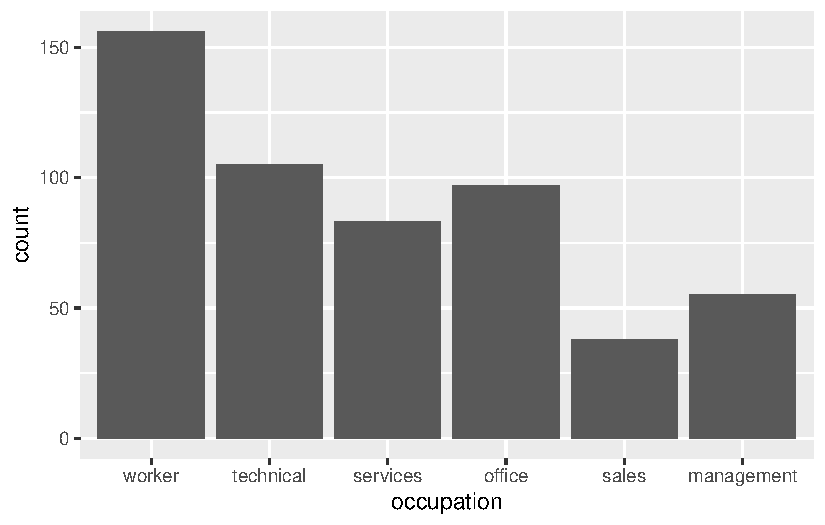
\includegraphics[keepaspectratio]{basicstats_files/figure-pdf/unnamed-chunk-2-1.pdf}}

In three lines of code, we have created a very barebones bar chart for
our data. How does this code work?

\begin{itemize}
\tightlist
\item
  \texttt{CPS1985\ \textbar{}\textgreater{}} pipes the CPS data into the
  \texttt{ggplot()} function.
\item
  The \texttt{ggplot()} sets the \emph{aesthetic} for the overall graph
  with the \texttt{aes()} option. I want the x dimension to be the
  occupation variable, hence \texttt{aes(x\ =\ occupation)}. Because the
  default statistic of a bar chart is to give me counts of each group, I
  don't need to define any other aesthetics.
\item
  The \texttt{+} at the end of the line allows me to add a layer to my
  graph.

  \begin{itemize}
  \tightlist
  \item
    This is also a good place to remind you of the ``one line, one
    thing'' rule from Chapter~\ref{sec-wrangling}!
  \end{itemize}
\item
  \texttt{geom\_bar()} creates a basic bar chart. The prefix
  \texttt{geom\_} tells us that we are adding a \emph{geometry} layer,
  and our \emph{geometry} is that of a \emph{bar chart}.
\end{itemize}

\begin{tcolorbox}[enhanced jigsaw, colframe=quarto-callout-tip-color-frame, breakable, arc=.35mm, bottomtitle=1mm, bottomrule=.15mm, colbacktitle=quarto-callout-tip-color!10!white, rightrule=.15mm, colback=white, opacityback=0, opacitybacktitle=0.6, coltitle=black, left=2mm, toptitle=1mm, toprule=.15mm, titlerule=0mm, leftrule=.75mm, title=\textcolor{quarto-callout-tip-color}{\faLightbulb}\hspace{0.5em}{Data Storytelling: The Three Stages of Graph Evolution}]

In Chapter~\ref{sec-litprog} Literate Programming, I suggested that
documents evolve through stages. So too do graphs.

There's a very similar three-stage approach you might think of with
graphs too:

\begin{itemize}
\item
  Stage 1: Data to Plot - Here you ask the question, ``does this show
  what I think it shows?'' There is no need to mess around with making
  everything look pretty, this is just you exploring the data, trying to
  find the graph that does the best job of telling the story you want to
  tell with the data. The focus here is typically on getting the
  aesthetics and layers right.
\item
  Stage 2: Basic Communication - The next stage is to ask ``can someone
  else understand this?'' In this stage, you need to ensure that the
  data is labeled, titles are on your graph, and so on. This is when you
  start adding theme elements, particularly label options.
\item
  Stage 3: Publication Ready - The final stage is to ask the question of
  ``would I put this in a presentation/report?'' This step is putting
  the final polish on your graph, ensuring your colors are right (are
  you on brand? Do you need to choose colorblind friendly colors?), etc.
\end{itemize}

Throughout this chapter, I'll usually show Stage 1 and Stage 2 examples,
with occasional Stage 3 examples to show what's possible.

\end{tcolorbox}

You might be wondering why we use \texttt{\textbar{}\textgreater{}} to
connect \texttt{CPS1985} to \texttt{ggplot()} but then use \texttt{+} to
add layers to our graph. Here's the logic:

\begin{itemize}
\item
  Use \texttt{\textbar{}\textgreater{}} (pipe) when you're passing data
  from one step to the next. Think ``take this data \textbf{and then} do
  something with it.''
\item
  Use \texttt{+} (plus) when you're building up layers within ggplot.
  Think ``add this layer \textbf{on top of} what I already have.''
\end{itemize}

So \texttt{CPS1985\ \ \textbar{}\textgreater{}\ \ ggplot()} means ``take
the CPS1985 data and pipe it into ggplot,'' while
\texttt{ggplot()\ +\ geom\_bar()} means ``start with a ggplot and add a
bar chart layer on top.'' As a general rule, you always use
\texttt{\textbar{}\textgreater{}} for \texttt{dplyr} data wrangling
tasks, but use \texttt{+} for \texttt{ggplot()} visualization building.

While we have a perfectly functional graph, it is not that pretty. I
don't love the default gray background that \texttt{ggplot()} gives,
nothing is labeled, and so forth. Let's fix this up with a few more
layers and theme options:

\begin{Shaded}
\begin{Highlighting}[]
\NormalTok{CPS1985 }\SpecialCharTok{|\textgreater{}} 
  \FunctionTok{ggplot}\NormalTok{(}\FunctionTok{aes}\NormalTok{(}\AttributeTok{x =}\NormalTok{ occupation)) }\SpecialCharTok{+}
  \FunctionTok{geom\_bar}\NormalTok{() }\SpecialCharTok{+}
  \FunctionTok{theme\_minimal}\NormalTok{() }\SpecialCharTok{+}
  \FunctionTok{labs}\NormalTok{(}\AttributeTok{title =} \StringTok{"Distribution of Occupations"}\NormalTok{, }
       \AttributeTok{caption =} \StringTok{"Random sample of 534 observations from 1985 CPS"}\NormalTok{,}
       \AttributeTok{x =} \StringTok{""}\NormalTok{, }
       \AttributeTok{y =} \StringTok{"Number of Observations"}\NormalTok{)}
\end{Highlighting}
\end{Shaded}

\pandocbounded{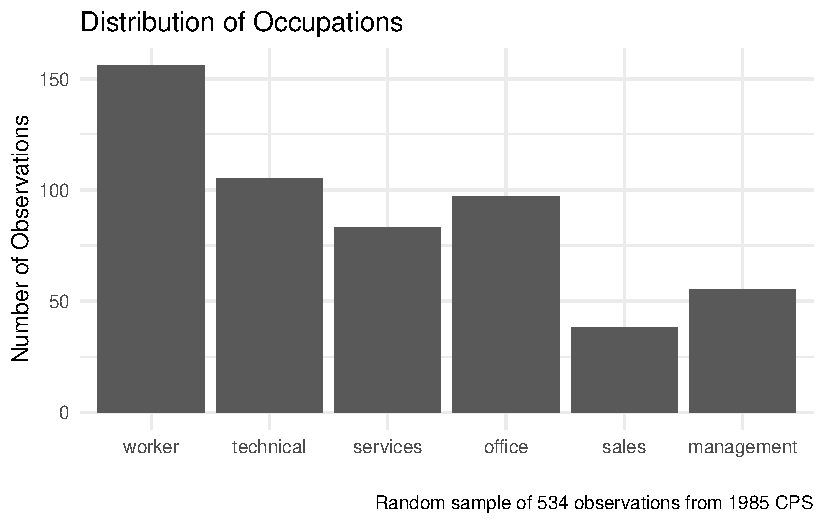
\includegraphics[keepaspectratio]{basicstats_files/figure-pdf/unnamed-chunk-3-1.pdf}}

This code starts with the barebones code from above and augments it to
add some additional elements and layers, and with just a few more lines
the graph is a lot more readable. Here is what got added:

\begin{itemize}
\item
  \texttt{theme\_minimal()}: There are a few ``all-in-one'' themes built
  into \texttt{ggplot()} that alter the appearance of the graph
  considerably, and \texttt{theme\_minimal()} is probably my favorite
  general-purpose theme. The other themes are \texttt{theme\_gray()}
  (technically the default theme), \texttt{theme\_bw()},
  \texttt{theme\_linedraw()}, \texttt{theme\_light()},
  \texttt{theme\_dark()}, \texttt{theme\_classic()}, and
  \texttt{theme\_void()}. It's worth taking a look at these to see which
  you prefer.
\item
  \texttt{labs()}: Short for \textbf{labels}, specifying labels and
  titles are essential for readability. By default, \texttt{ggplot()}
  labels axes with the variable names from your dataset, but these
  aren't always reader-friendly. Here we've added a title, caption, and
  changed the y-axis from ``count'' to the more intuitive ``Number of
  Observations.'' For the x-axis, since our title already specifies
  we're looking at occupations, the default ``occupation'' label is
  redundant, so \texttt{x\ =\ ""} removes it entirely.
\end{itemize}

\begin{tcolorbox}[enhanced jigsaw, colframe=quarto-callout-tip-color-frame, breakable, arc=.35mm, bottomtitle=1mm, bottomrule=.15mm, colbacktitle=quarto-callout-tip-color!10!white, rightrule=.15mm, colback=white, opacityback=0, opacitybacktitle=0.6, coltitle=black, left=2mm, toptitle=1mm, toprule=.15mm, titlerule=0mm, leftrule=.75mm, title=\textcolor{quarto-callout-tip-color}{\faLightbulb}\hspace{0.5em}{Data Storytelling: The Self-Contained Graph Test}]

A well-designed graph should tell a complete story on its own. If you
handed your graph to a friend or colleague or teacher with no context,
could they understand what they're looking at and what point you're
making? Good graphs don't require you to be standing there explaining
what everything means.

To illustrate this point, I'm going to do things a bit backwards for a
moment. I'll start by showing you a graph without any of the code that
wrangles the data so you can't cheat and look up the data yourself (I
mean you can still cheat by scrolling down a bit but whatever). Look a
look at this graph; what does it show?

\begin{Shaded}
\begin{Highlighting}[]
\NormalTok{sb }\SpecialCharTok{|\textgreater{}} 
  \FunctionTok{ggplot}\NormalTok{(}\FunctionTok{aes}\NormalTok{(}\AttributeTok{y =}\NormalTok{ drivers, }\AttributeTok{x =}\NormalTok{ year)) }\SpecialCharTok{+} 
  \FunctionTok{geom\_line}\NormalTok{()}
\end{Highlighting}
\end{Shaded}

\pandocbounded{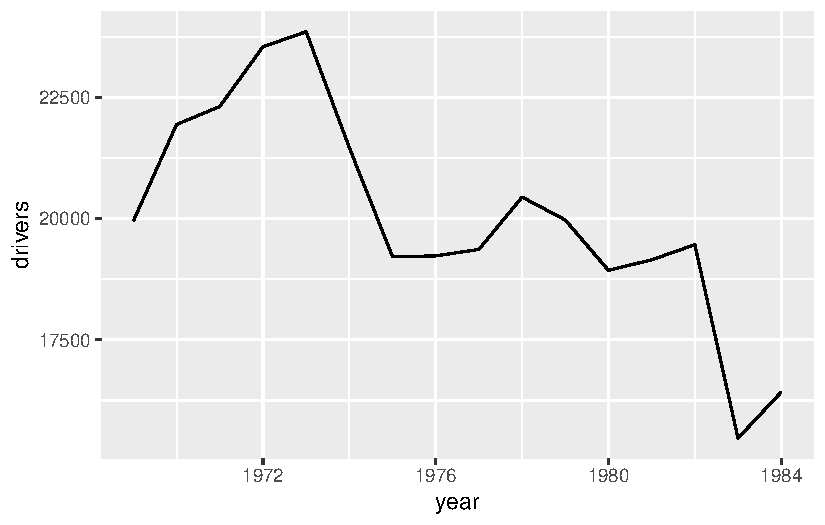
\includegraphics[keepaspectratio]{basicstats_files/figure-pdf/unnamed-chunk-5-1.pdf}}

Based on the default labeling, it looks like a time trend of some sort
because the x-axis is labeled ``year'', but drivers could be anything.
Something about automobiles, maybe? Traffic safety or number of people
getting their licenses? Number of taxi drivers? Or maybe some other kind
of drivers. Perhaps we are looking at the data for sales on golf clubs
or screwdrivers? If screwdrivers, the tool or the cocktail? And for all
of these, where? US? Worldwide? Who knows?

This graph cannot stand alone. And generally speaking, it's not good
enough to have a thorough description of the graph in the text around
your graph (although you do need that!). A graph needs to tell a
self-contained story, so let's put some labels in here:

\begin{Shaded}
\begin{Highlighting}[]
\NormalTok{sb }\SpecialCharTok{|\textgreater{}} 
  \FunctionTok{ggplot}\NormalTok{(}\FunctionTok{aes}\NormalTok{(}\AttributeTok{y =}\NormalTok{ drivers, }\AttributeTok{x =}\NormalTok{ year)) }\SpecialCharTok{+} 
  \FunctionTok{geom\_line}\NormalTok{() }\SpecialCharTok{+}
  \FunctionTok{geom\_vline}\NormalTok{(}\AttributeTok{xintercept =} \DecValTok{1983}\NormalTok{, }\AttributeTok{linetype =} \StringTok{"dashed"}\NormalTok{) }\SpecialCharTok{+}
  \FunctionTok{theme\_classic}\NormalTok{() }\SpecialCharTok{+}
  \FunctionTok{labs}\NormalTok{(}\AttributeTok{title =} \StringTok{"UK Traffic Fatalities, 1969 {-} 1984"}\NormalTok{, }
       \AttributeTok{subtitle =} \StringTok{"Mandatory Seatbelt Law Goes Into Effect January 1983"}\NormalTok{,}
       \AttributeTok{y =} \StringTok{"Traffic Fatalties"}\NormalTok{, }
       \AttributeTok{x =} \StringTok{"Year"}\NormalTok{)}
\end{Highlighting}
\end{Shaded}

\pandocbounded{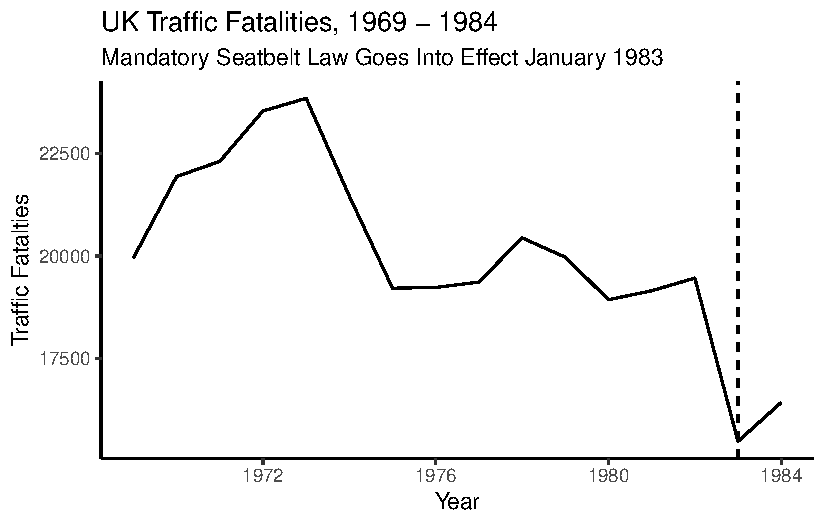
\includegraphics[keepaspectratio]{basicstats_files/figure-pdf/unnamed-chunk-6-1.pdf}}

With just a little more effort, we can see what the graph is showing.
All I really added was a title/subtitle, axis labels, and the dashed
line to show the date when compulsory wearing of seatbelts went into
effect. And now, the graph now tells a story.

As promised, here is the code that generates the data from the
\texttt{Seatbelts} dataset built into R. The original data is monthly
and not in a format that the \texttt{tidyverse} likes (\texttt{dplyr}
and \texttt{ggplot()} don't play nicely with data configured for the
sorts of Time Series stuff we will see in Chapter~\ref{sec-timeseries});
most of what you see here is just an application of the data wrangling
techniques from Chapter~\ref{sec-wrangling}. It changes the data type
(that's the \texttt{as.tibble()} line), creates a year variable (that's
the \texttt{mutate()}), and then converts the monthly data into annual
data:

\begin{Shaded}
\begin{Highlighting}[]
\FunctionTok{data}\NormalTok{(Seatbelts)}
\NormalTok{sb }\OtherTok{\textless{}{-}}\NormalTok{ Seatbelts }\SpecialCharTok{|\textgreater{}} 
  \FunctionTok{as.tibble}\NormalTok{() }\SpecialCharTok{|\textgreater{}} 
  \FunctionTok{mutate}\NormalTok{(}\AttributeTok{year =} \FunctionTok{floor}\NormalTok{((}\DecValTok{1969} \SpecialCharTok{+}\NormalTok{ (}\FunctionTok{row\_number}\NormalTok{()}\SpecialCharTok{{-}}\DecValTok{1}\NormalTok{)}\SpecialCharTok{/}\DecValTok{12}\NormalTok{))) }\SpecialCharTok{|\textgreater{}} 
  \FunctionTok{group\_by}\NormalTok{(year) }\SpecialCharTok{|\textgreater{}} 
  \FunctionTok{mutate}\NormalTok{(}\AttributeTok{drivers =} \FunctionTok{sum}\NormalTok{(drivers)) }\SpecialCharTok{|\textgreater{}} 
  \FunctionTok{select}\NormalTok{(year, drivers) }\SpecialCharTok{|\textgreater{}} 
  \FunctionTok{distinct}\NormalTok{()}
\end{Highlighting}
\end{Shaded}

\end{tcolorbox}

Our occupation graph is fine, but suppose we really want to elevate this
graph. Let's think about what we might need to do to make this
publication worthy. First, we might think about color. Since this is
Data from the US Census, let's imagine that we want to use the official
colors of the US Census. I went online and grabbed the official version
of the color blue they list in their style guide ({``US Census Bureau:
Corporate Identity and Branding Standards''} 2019), which is
\texttt{\#205493}, so we can include that as a color in the graph. I'm
going to add a black outline to the bars to make them pop as well; since
black is one of the many ``named colors'' in R, we'll just refer to it
as \texttt{"black"} (If you want to learn more about named colors, try
running \texttt{demo("colors")}!). We might also think to flip the
orientation (horizontal bars instead of vertical bars), clean up the
gridline situation, remove some empty space between the axis and the
beginning of the bars, and alphabetize and capitalize the occupations:

\begin{Shaded}
\begin{Highlighting}[]
\NormalTok{CPS1985 }\SpecialCharTok{|\textgreater{}} 
  \FunctionTok{mutate}\NormalTok{(}\AttributeTok{occupation =} \FunctionTok{fct\_rev}\NormalTok{(}\FunctionTok{fct\_relevel}\NormalTok{(occupation, }\FunctionTok{sort}\NormalTok{(}\FunctionTok{levels}\NormalTok{(occupation))))) }\SpecialCharTok{|\textgreater{}} 
  \FunctionTok{mutate}\NormalTok{(}\AttributeTok{occupation =} \FunctionTok{fct\_relabel}\NormalTok{(occupation, str\_to\_title)) }\SpecialCharTok{|\textgreater{}} 
  \FunctionTok{ggplot}\NormalTok{(}\FunctionTok{aes}\NormalTok{(}\AttributeTok{y =}\NormalTok{ occupation)) }\SpecialCharTok{+}
  \FunctionTok{geom\_bar}\NormalTok{(}\AttributeTok{fill =} \StringTok{"\#205493"}\NormalTok{,}
           \AttributeTok{color =} \StringTok{"black"}\NormalTok{) }\SpecialCharTok{+}
  \FunctionTok{scale\_x\_continuous}\NormalTok{(}\AttributeTok{expand =} \FunctionTok{c}\NormalTok{(}\DecValTok{0}\NormalTok{,}\DecValTok{0}\NormalTok{)) }\SpecialCharTok{+}
  \FunctionTok{theme\_minimal}\NormalTok{() }\SpecialCharTok{+}
  \FunctionTok{theme}\NormalTok{(}\AttributeTok{panel.grid.major.y =} \FunctionTok{element\_blank}\NormalTok{()) }\SpecialCharTok{+}
  \FunctionTok{labs}\NormalTok{(}\AttributeTok{title =} \StringTok{"Distribution of Occupations"}\NormalTok{, }
       \AttributeTok{caption =} \StringTok{"Random sample of 534 observations from 1985 CPS"}\NormalTok{,}
       \AttributeTok{y =} \StringTok{""}\NormalTok{, }
       \AttributeTok{x =} \StringTok{"Number of Observations"}\NormalTok{)}
\end{Highlighting}
\end{Shaded}

\pandocbounded{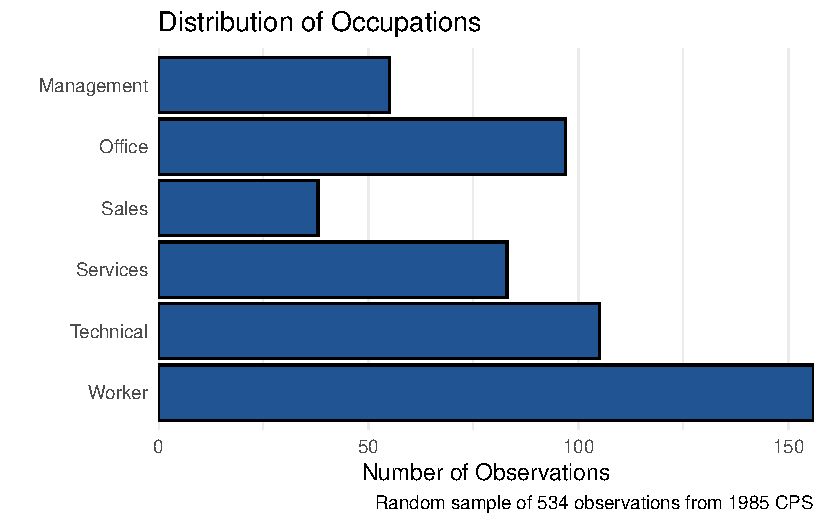
\includegraphics[keepaspectratio]{basicstats_files/figure-pdf/unnamed-chunk-8-1.pdf}}

Real talk: the code complexity just took a bit of a jump here. The
\texttt{fct\_} functions are doing some behind-the-scenes magic to
alphabetize and capitalize the occupation labels, but don't stress about
understanding them right now. Here's the thing about making graphs in R:
it follows the classic 80-20 rule. Getting from ugly to pretty good
takes about 20\% of the effort and is usually pretty easy, but going
from pretty good to magazine-quality? That's the other 80\% right there,
and it can require some serious code gymnastics. It's why you don't do
it until you are sure about the basics of your graph. The payoff is
worth it though; this graph is way more polished than our earlier
versions!

The other primary way to display categorical data is via a pie chart.
Fun fact: many people who study data visualization believe that a pie
chart is a really awful way to graph data. Case in point: the folks
behind \texttt{ggplot2} did not provide an easy way of making a pie
chart, they know better!

\begin{center}

\includegraphics[width=0.5\linewidth,height=\textheight,keepaspectratio]{images/normalpie.jpg}
\end{center}

Base R, however, has no such qualms about letting you make questionable
life choices. Making a pie chart is quite simple and requires two steps.
First, you need to use the \texttt{table()} function to create the
actual data to be graphed:

\begin{Shaded}
\begin{Highlighting}[]
\NormalTok{jobtype }\OtherTok{\textless{}{-}} \FunctionTok{table}\NormalTok{(CPS1985}\SpecialCharTok{$}\NormalTok{occupation)}
\NormalTok{jobtype}
\end{Highlighting}
\end{Shaded}

\begin{verbatim}

    worker  technical   services     office      sales management 
       156        105         83         97         38         55 
\end{verbatim}

As you can see, \texttt{table()} creates a cross-tabulation table of the
variable you feed it. From there, the base R pie chart is generated with
the \texttt{pie()} function:

\begin{Shaded}
\begin{Highlighting}[]
\FunctionTok{pie}\NormalTok{(jobtype)}
\end{Highlighting}
\end{Shaded}

\pandocbounded{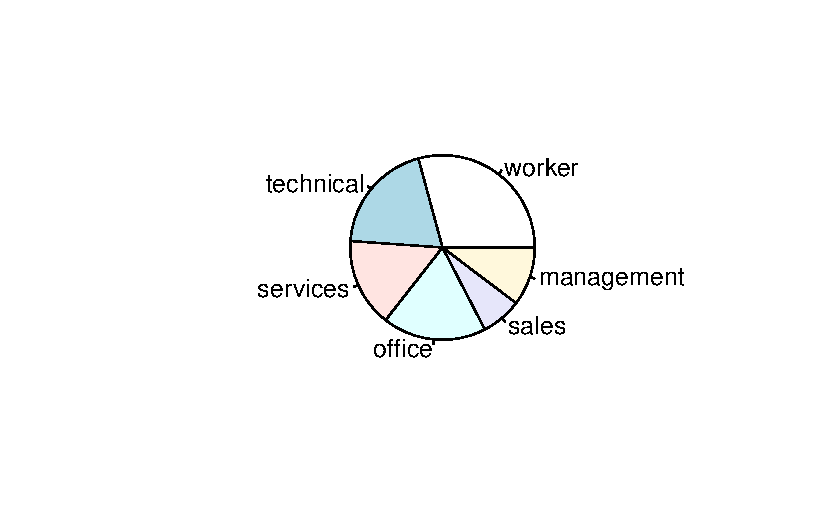
\includegraphics[keepaspectratio]{basicstats_files/figure-pdf/unnamed-chunk-11-1.pdf}}

In base R, it is easy as pie. Ugly, but easy. For what it's worth, the
base R version of the bar chart requires the same initial step of making
the cross-tab and then plugging it into the \texttt{barplot()} function.

\begin{Shaded}
\begin{Highlighting}[]
\FunctionTok{barplot}\NormalTok{(jobtype)}
\end{Highlighting}
\end{Shaded}

\pandocbounded{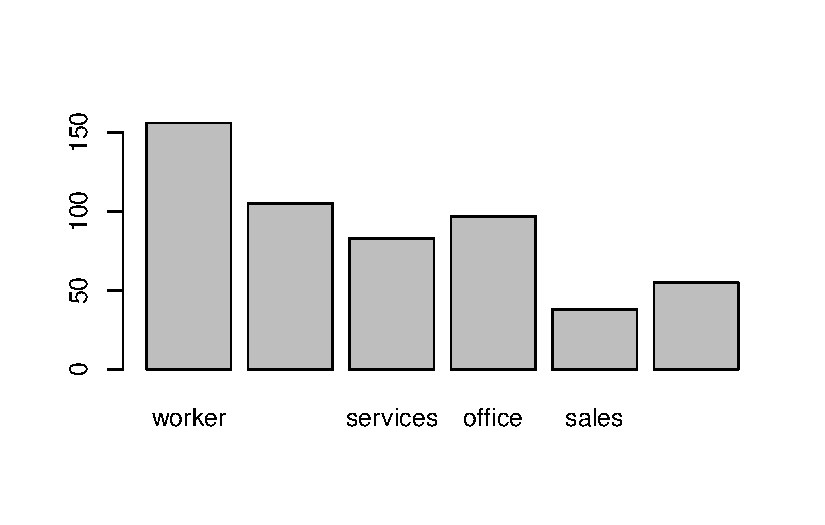
\includegraphics[keepaspectratio]{basicstats_files/figure-pdf/unnamed-chunk-12-1.pdf}}

\begin{tcolorbox}[enhanced jigsaw, colframe=quarto-callout-tip-color-frame, breakable, arc=.35mm, bottomtitle=1mm, bottomrule=.15mm, colbacktitle=quarto-callout-tip-color!10!white, rightrule=.15mm, colback=white, opacityback=0, opacitybacktitle=0.6, coltitle=black, left=2mm, toptitle=1mm, toprule=.15mm, titlerule=0mm, leftrule=.75mm, title=\textcolor{quarto-callout-tip-color}{\faLightbulb}\hspace{0.5em}{Data Storytelling: Why Pie Charts Are Evil (A Scientific Demonstration)}]

I am firmly on team ``Pie Charts are Evil,'' and I'm about to
demonstrate why with a simple experiment. Here's the thing: our brains
just aren't wired to accurately compare angles and pie slices, which is
exactly what pie charts force us to do.

Let me show you what I mean. I'll simulate rolling 100 dice and then
compare how pie charts vs.~bar charts handle the results:

\begin{Shaded}
\begin{Highlighting}[]
\FunctionTok{set.seed}\NormalTok{(}\DecValTok{8675309}\NormalTok{) }\CommentTok{\# Jenny!}
\NormalTok{dice\_rolls }\OtherTok{\textless{}{-}} \FunctionTok{sample}\NormalTok{(}\DecValTok{1}\SpecialCharTok{:}\DecValTok{6}\NormalTok{, }\DecValTok{100}\NormalTok{, }\AttributeTok{replace =} \ConstantTok{TRUE}\NormalTok{)}
\NormalTok{dice\_counts }\OtherTok{\textless{}{-}} \FunctionTok{table}\NormalTok{(dice\_rolls)}
\end{Highlighting}
\end{Shaded}

Now, which visualization actually lets you see which number came up most
often?

Starting with the pie chart:

\begin{Shaded}
\begin{Highlighting}[]
\FunctionTok{pie}\NormalTok{(dice\_counts)}
\end{Highlighting}
\end{Shaded}

\pandocbounded{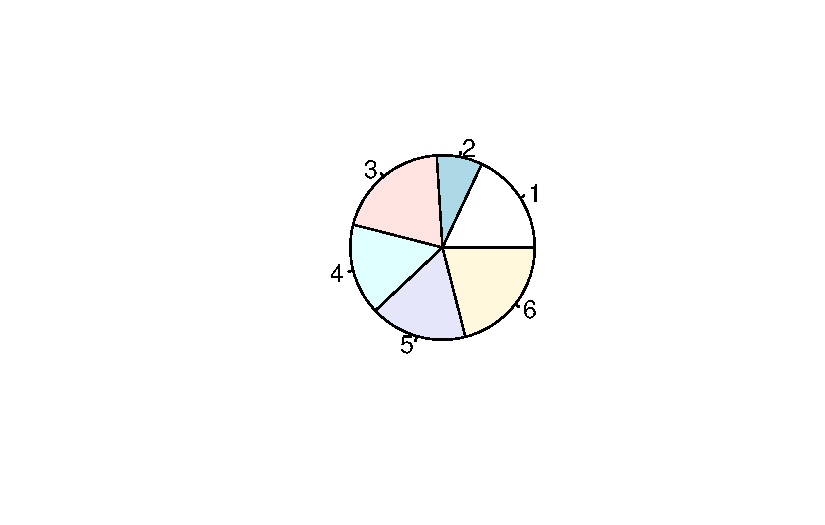
\includegraphics[keepaspectratio]{basicstats_files/figure-pdf/unnamed-chunk-14-1.pdf}}

Seriously, can you tell the difference between the slices for 3 and 6?
What about 1, 4, and 5? Your brain is working overtime trying to compare
these curved slices, and it's probably getting it wrong.

Now, compare this to the bar chart:

\begin{Shaded}
\begin{Highlighting}[]
\FunctionTok{barplot}\NormalTok{(dice\_counts)}
\end{Highlighting}
\end{Shaded}

\pandocbounded{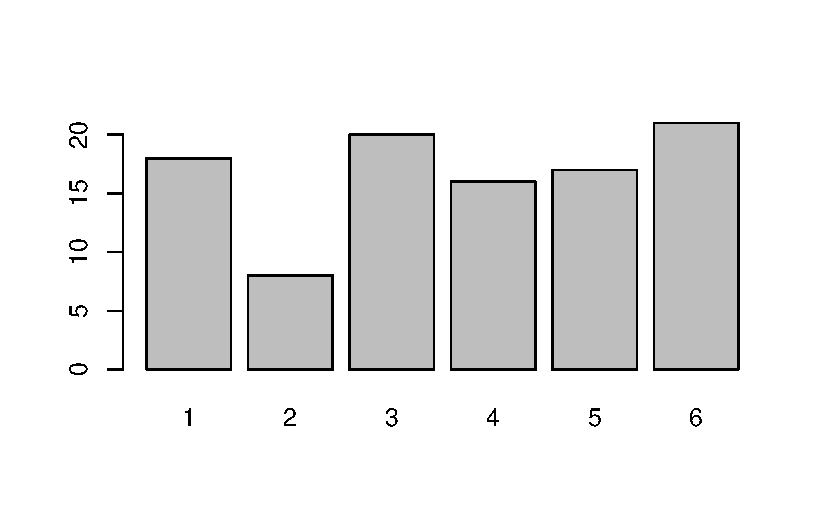
\includegraphics[keepaspectratio]{basicstats_files/figure-pdf/unnamed-chunk-15-1.pdf}}

The differences are immediately obvious! Your brain is excellent at
comparing heights - that's what bar charts give you to work with.

Just to confirm what the bar chart made obvious (but the pie chart made
non-obvious!), here are the actual counts:

\begin{longtable}[]{@{}lr@{}}
\caption{Simulated Dice Roll Results}\tabularnewline
\toprule\noalign{}
Die Face & Count \\
\midrule\noalign{}
\endfirsthead
\toprule\noalign{}
Die Face & Count \\
\midrule\noalign{}
\endhead
\bottomrule\noalign{}
\endlastfoot
1 & 18 \\
2 & 8 \\
3 & 20 \\
4 & 16 \\
5 & 17 \\
6 & 21 \\
\end{longtable}

BTW, this isn't just me being a data visualization snob. There's actual
research (e.g. Cleveland and McGill 1984) showing that people make more
errors reading pie charts than bar charts. When you use a pie chart,
you're literally making your audience work harder to understand your
data. If you get to choose the presentation type, Why would you do that
to them?

\end{tcolorbox}

With some work, pie charts can also be made using \texttt{ggplot()}.
However, I feel it is my responsibility to discourage you from making
poor life decisions, and making pie charts is among the worst decisions
one can make in life. Seriously, if you are making a pie chart, you
really ought to be asking yourself what set of awful decisions did you
make in your life that led up to a point where you are currently making
a pie chart.

But, I get it. Maybe your boss or teacher or whomever really wants a pie
chart. Definitely not you, you are better than that.

\begin{figure}

\centering{

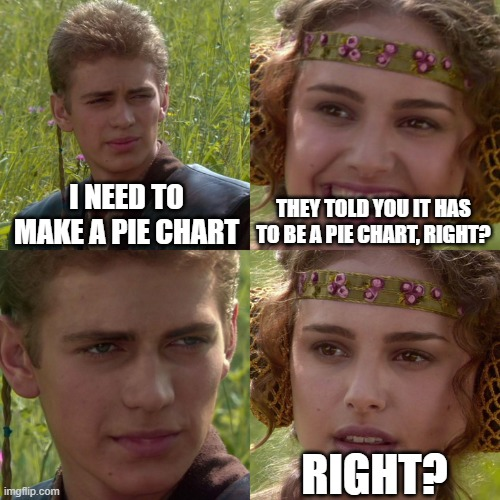
\includegraphics[width=0.7\linewidth,height=\textheight,keepaspectratio]{images/anakinpadmepie.jpg}

}

\caption{\label{fig-padme-anakin}}

\end{figure}%

If it can be done, then I suppose it will be done! Making pie charts in
\texttt{ggplot()} requires us to make a special version of a stacked
barchart, which we will discuss later, so the \texttt{ggplot()} based
instructions on making \hyperref[pie-charts]{Pie Charts} will have to
wait until a little later in the chapter.

\subsection{Boxplots}\label{boxplots}

A \textbf{boxplot} (sometimes called a \textbf{Box and Whiskers Plot})
is a very common way of displaying the distribution of numerical data by
showing the 0th, 25th, 50th (median), and 75th percentiles as a box,
with whiskers extending to show the range of the data (excluding
outliers). I usually skip them when I teach intro to stats because they
are stupidly hard to make in Excel. But they are a snap in R.

Let's create a boxplot of the \texttt{wage} variable in the
\texttt{CPS1985} dataset we've been using all chapter. If we want our
boxplot to be oriented vertically, we can set \texttt{y\ =\ wage} (for a
horizontal orientation we would set \texttt{x\ =\ wage}) as our
aesthetic in \texttt{ggplot()}. A boxplot is a type of geometry, hence
\texttt{geom\_boxplot()}.

\begin{Shaded}
\begin{Highlighting}[]
\NormalTok{CPS1985 }\SpecialCharTok{|\textgreater{}} 
  \FunctionTok{ggplot}\NormalTok{(}\FunctionTok{aes}\NormalTok{(}\AttributeTok{y =}\NormalTok{ wage)) }\SpecialCharTok{+}
  \FunctionTok{geom\_boxplot}\NormalTok{() }
\end{Highlighting}
\end{Shaded}

\pandocbounded{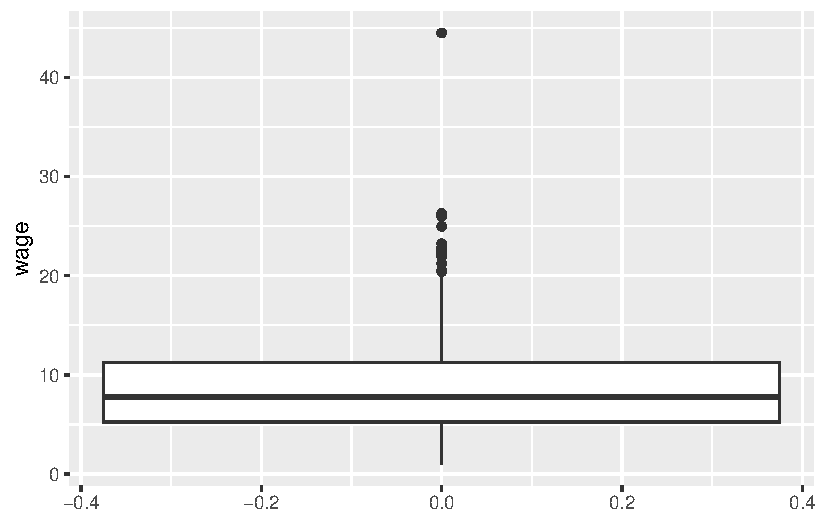
\includegraphics[keepaspectratio]{basicstats_files/figure-pdf/unnamed-chunk-18-1.pdf}}

The boxplot shows us the 1st-3rd quartiles of the data, and the dots are
the outliers. If we want to turn our boxplot into a box and whiskers
plot, we need to add our whiskers with the \texttt{stat\_boxplot} layer,
as seen here:

\begin{Shaded}
\begin{Highlighting}[]
\NormalTok{CPS1985 }\SpecialCharTok{|\textgreater{}} 
  \FunctionTok{ggplot}\NormalTok{(}\FunctionTok{aes}\NormalTok{(}\AttributeTok{y =}\NormalTok{ wage)) }\SpecialCharTok{+}
  \FunctionTok{stat\_boxplot}\NormalTok{(}\AttributeTok{geom =} \StringTok{"errorbar"}\NormalTok{, }\AttributeTok{width =} \FloatTok{0.5}\NormalTok{) }\SpecialCharTok{+}
  \FunctionTok{geom\_boxplot}\NormalTok{() }
\end{Highlighting}
\end{Shaded}

\pandocbounded{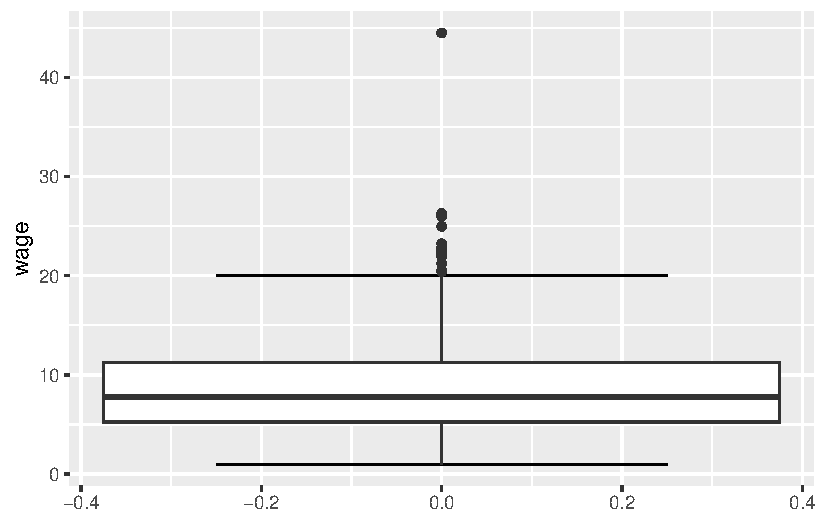
\includegraphics[keepaspectratio]{basicstats_files/figure-pdf/unnamed-chunk-19-1.pdf}}

Finally, let's clean this up just a little:

\begin{Shaded}
\begin{Highlighting}[]
\NormalTok{CPS1985 }\SpecialCharTok{|\textgreater{}} 
  \FunctionTok{ggplot}\NormalTok{(}\FunctionTok{aes}\NormalTok{(}\AttributeTok{y =}\NormalTok{ wage)) }\SpecialCharTok{+}
  \FunctionTok{stat\_boxplot}\NormalTok{(}\AttributeTok{geom =} \StringTok{"errorbar"}\NormalTok{, }\AttributeTok{width =} \FloatTok{0.5}\NormalTok{) }\SpecialCharTok{+} 
  \FunctionTok{geom\_boxplot}\NormalTok{(}\AttributeTok{fill =} \StringTok{"lightblue"}\NormalTok{) }\SpecialCharTok{+}
  \FunctionTok{theme\_minimal}\NormalTok{() }\SpecialCharTok{+}
  \FunctionTok{labs}\NormalTok{(}\AttributeTok{title =} \StringTok{"Distribution of Wage Variable"}\NormalTok{,}
       \AttributeTok{subtitle =} \StringTok{"CPS1985 dataset from AER package"}\NormalTok{,}
       \AttributeTok{y =} \StringTok{"Hourly Wage"}\NormalTok{,}
       \AttributeTok{x =} \StringTok{""}\NormalTok{)}
\end{Highlighting}
\end{Shaded}

\pandocbounded{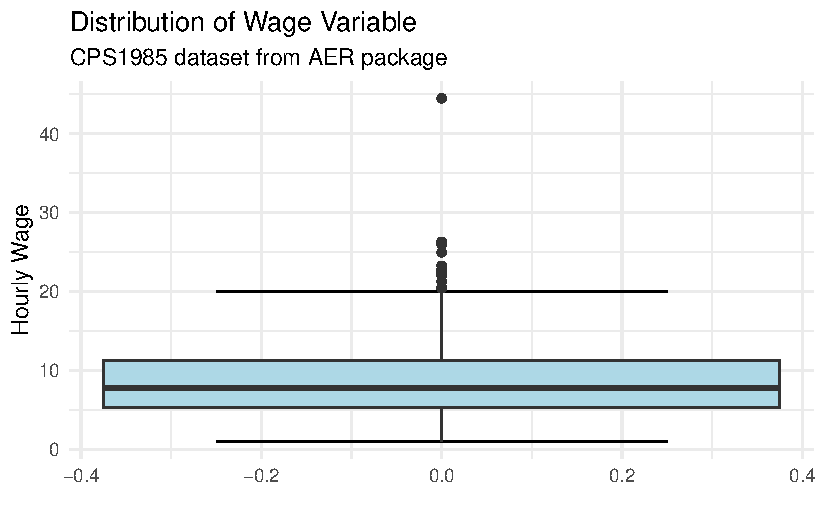
\includegraphics[keepaspectratio]{basicstats_files/figure-pdf/unnamed-chunk-20-1.pdf}}

\begin{tcolorbox}[enhanced jigsaw, colframe=quarto-callout-tip-color-frame, breakable, arc=.35mm, bottomtitle=1mm, bottomrule=.15mm, colbacktitle=quarto-callout-tip-color!10!white, rightrule=.15mm, colback=white, opacityback=0, opacitybacktitle=0.6, coltitle=black, left=2mm, toptitle=1mm, toprule=.15mm, titlerule=0mm, leftrule=.75mm, title=\textcolor{quarto-callout-tip-color}{\faLightbulb}\hspace{0.5em}{Data Storytelling: Layer Order Matters}]

You may have noticed that, when I added the \texttt{stat\_boxplot()}, I
put it \emph{before} the \texttt{geom\_boxplot()}, and perhaps you
wondered if it mattered. Turns out that yes, it did. When building
\texttt{ggplot()} visualizations, layers are placed on top of each other
in order, and I really wanted the \texttt{geom\_boxplot()} \emph{on top
of} the \texttt{stat\_boxplot()}. Let's take a look at the difference.

First, let's see what the individual parts of the box and whiskers plot
are doing; I'm using the \texttt{fill\ =\ "transparent"} and
\texttt{color\ =\ "transparent"} arguments (\texttt{fill} is for areas,
\texttt{color} is for lines and points) to make different pieces of the
graph transparent:

\begin{Shaded}
\begin{Highlighting}[]
\CommentTok{\# Graph 1 code}
\NormalTok{CPS1985 }\SpecialCharTok{|\textgreater{}} 
  \FunctionTok{ggplot}\NormalTok{(}\FunctionTok{aes}\NormalTok{(}\AttributeTok{y =}\NormalTok{ wage)) }\SpecialCharTok{+}
  \FunctionTok{stat\_boxplot}\NormalTok{(}\AttributeTok{geom =} \StringTok{"errorbar"}\NormalTok{,  }\AttributeTok{color =} \StringTok{"transparent"}\NormalTok{, }\AttributeTok{width =} \FloatTok{0.5}\NormalTok{) }\SpecialCharTok{+} 
  \FunctionTok{geom\_boxplot}\NormalTok{(}\AttributeTok{fill =} \StringTok{"lightblue"}\NormalTok{, }\AttributeTok{color =} \StringTok{"black"}\NormalTok{) }\SpecialCharTok{+}
  \FunctionTok{theme\_minimal}\NormalTok{() }\SpecialCharTok{+}
  \FunctionTok{labs}\NormalTok{(}\AttributeTok{title =} \StringTok{"Just the Boxplot"}\NormalTok{)}
\CommentTok{\# Graph 2 code  }
\NormalTok{CPS1985 }\SpecialCharTok{|\textgreater{}} 
  \FunctionTok{ggplot}\NormalTok{(}\FunctionTok{aes}\NormalTok{(}\AttributeTok{y =}\NormalTok{ wage)) }\SpecialCharTok{+}
  \FunctionTok{geom\_boxplot}\NormalTok{(}\AttributeTok{fill =} \StringTok{"transparent"}\NormalTok{, }\AttributeTok{color =} \StringTok{"transparent"}\NormalTok{) }\SpecialCharTok{+}
  \FunctionTok{stat\_boxplot}\NormalTok{(}\AttributeTok{geom =} \StringTok{"errorbar"}\NormalTok{, }\AttributeTok{width =} \FloatTok{0.5}\NormalTok{) }\SpecialCharTok{+} 
  \FunctionTok{theme\_minimal}\NormalTok{() }\SpecialCharTok{+}
  \FunctionTok{labs}\NormalTok{(}\AttributeTok{title =} \StringTok{"Just the Whiskers"}\NormalTok{)}
\end{Highlighting}
\end{Shaded}

\begin{figure}[H]

\begin{minipage}{0.50\linewidth}

\begin{figure}[H]

{\centering \pandocbounded{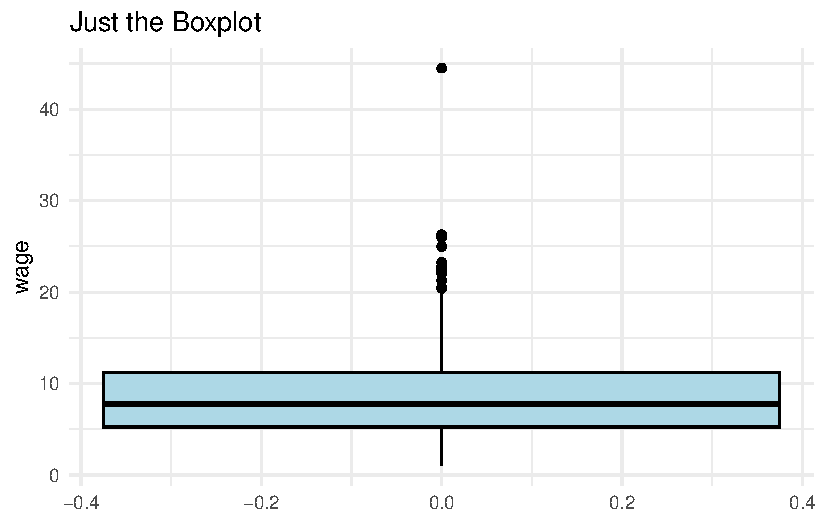
\includegraphics[keepaspectratio]{basicstats_files/figure-pdf/unnamed-chunk-21-1.pdf}}

}

\subcaption{Boxplot}

\end{figure}%

\end{minipage}%
%
\begin{minipage}{0.50\linewidth}

\begin{figure}[H]

{\centering \pandocbounded{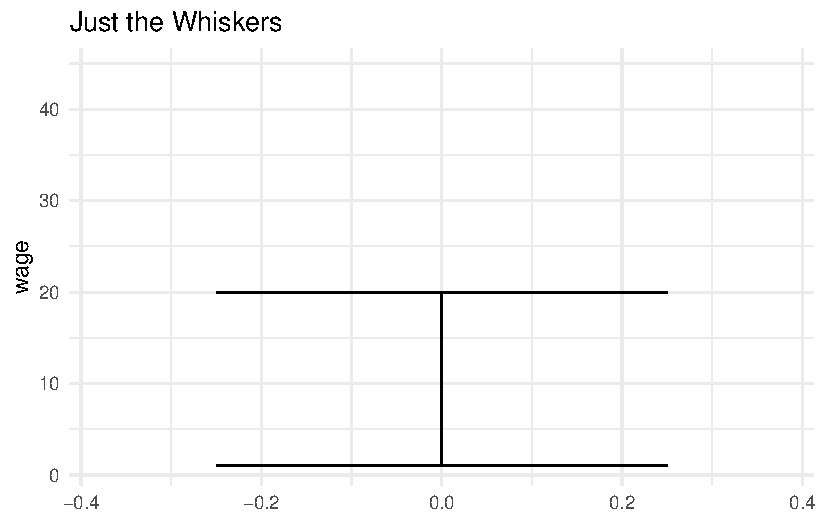
\includegraphics[keepaspectratio]{basicstats_files/figure-pdf/unnamed-chunk-21-2.pdf}}

}

\subcaption{Whiskers}

\end{figure}%

\end{minipage}%

\end{figure}%

Notice that the whiskers on the \texttt{geom\_boxplot()} don't go
through the box, but the \texttt{stat\_boxplot()} line is solid. So
let's see what happens when we switch the order of those lines.

\begin{Shaded}
\begin{Highlighting}[]
\CommentTok{\# Graph 1 code}
\NormalTok{CPS1985 }\SpecialCharTok{|\textgreater{}} 
  \FunctionTok{ggplot}\NormalTok{(}\FunctionTok{aes}\NormalTok{(}\AttributeTok{y =}\NormalTok{ wage)) }\SpecialCharTok{+}
  \FunctionTok{stat\_boxplot}\NormalTok{(}\AttributeTok{geom =} \StringTok{"errorbar"}\NormalTok{, }\AttributeTok{linewidth =} \DecValTok{1}\NormalTok{, }\AttributeTok{width =} \FloatTok{0.5}\NormalTok{) }\SpecialCharTok{+} 
  \FunctionTok{geom\_boxplot}\NormalTok{(}\AttributeTok{fill =} \StringTok{"lightblue"}\NormalTok{, }\AttributeTok{color =} \StringTok{"black"}\NormalTok{, }\AttributeTok{linewidth =} \DecValTok{1}\NormalTok{) }\SpecialCharTok{+}
  \FunctionTok{theme\_minimal}\NormalTok{() }\SpecialCharTok{+}
  \FunctionTok{labs}\NormalTok{(}\AttributeTok{title =} \StringTok{"Whiskers First"}\NormalTok{)}
\CommentTok{\# Graph 2 code  }
\NormalTok{CPS1985 }\SpecialCharTok{|\textgreater{}} 
  \FunctionTok{ggplot}\NormalTok{(}\FunctionTok{aes}\NormalTok{(}\AttributeTok{y =}\NormalTok{ wage)) }\SpecialCharTok{+}
  \FunctionTok{geom\_boxplot}\NormalTok{(}\AttributeTok{fill =} \StringTok{"lightblue"}\NormalTok{, }\AttributeTok{color =} \StringTok{"black"}\NormalTok{, }\AttributeTok{linewidth =} \DecValTok{1}\NormalTok{) }\SpecialCharTok{+}
  \FunctionTok{stat\_boxplot}\NormalTok{(}\AttributeTok{geom =} \StringTok{"errorbar"}\NormalTok{, }\AttributeTok{linewidth =} \DecValTok{1}\NormalTok{, }\AttributeTok{width =} \FloatTok{0.5}\NormalTok{) }\SpecialCharTok{+} 
  \FunctionTok{theme\_minimal}\NormalTok{() }\SpecialCharTok{+}
  \FunctionTok{labs}\NormalTok{(}\AttributeTok{title =} \StringTok{"Boxplot First"}\NormalTok{)}
\end{Highlighting}
\end{Shaded}

\begin{figure}[H]

\begin{minipage}{0.50\linewidth}

\begin{figure}[H]

{\centering \pandocbounded{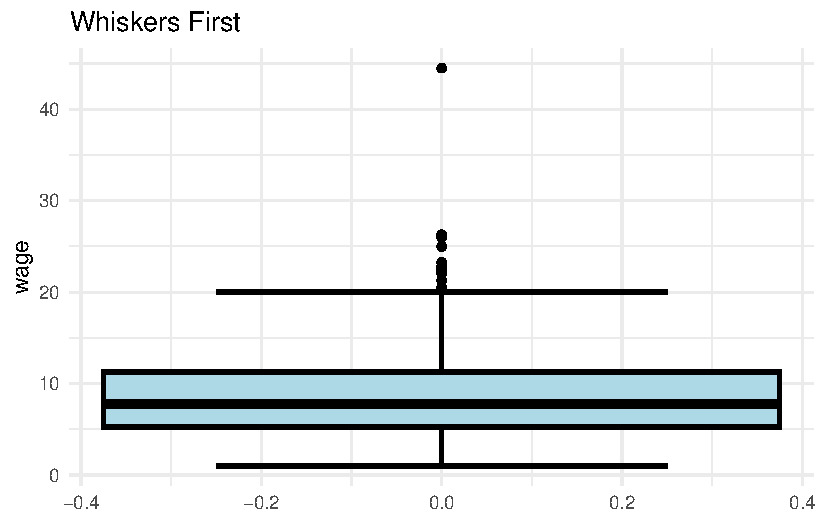
\includegraphics[keepaspectratio]{basicstats_files/figure-pdf/unnamed-chunk-22-1.pdf}}

}

\subcaption{Whiskers First (Preferred)}

\end{figure}%

\end{minipage}%
%
\begin{minipage}{0.50\linewidth}

\begin{figure}[H]

{\centering \pandocbounded{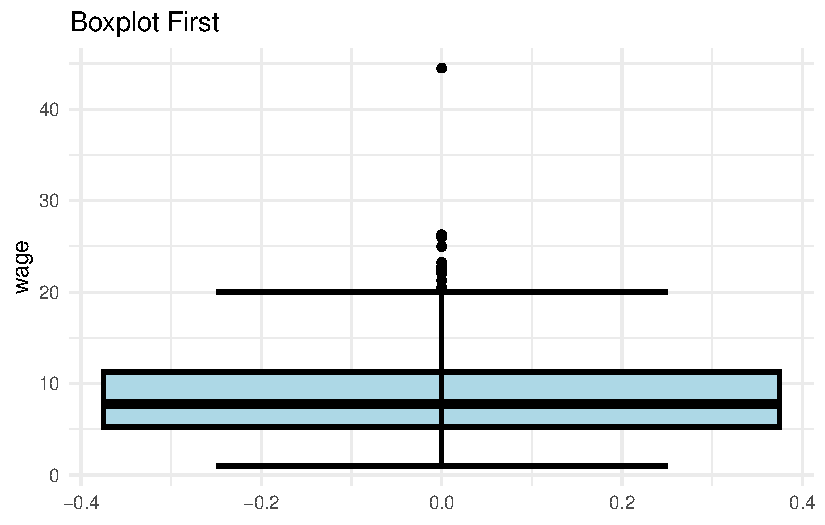
\includegraphics[keepaspectratio]{basicstats_files/figure-pdf/unnamed-chunk-22-2.pdf}}

}

\subcaption{Boxplot First (Not Preferred)}

\end{figure}%

\end{minipage}%

\end{figure}%

I thickened up the lines a bit to make the difference apparent. In the
version where the \texttt{stat\_boxplot()} comes first, the
\texttt{geom\_boxplot()} is placed on top of it and the vertical line is
covered. When \texttt{geom\_boxplot()} comes first, the full vertical
line can be seen because the \texttt{stat\_boxplot()} is drawn on top of
the boxplot itself. The former is the preferred look, which is why I did
it in the order I did.

But there is a useful lesson in this little digression. When making
graphs with \texttt{ggplot()}, all the work is done in order from top to
bottom, which means that \textbf{layer order matters}. Each new layer
gets painted on top of the previous ones, so elements added later can
cover up elements added earlier. Always think about what should be in
front and what should be in back when building complex visualizations.

\end{tcolorbox}

Typically, we wouldn't make a boxplot just to look at the distribution
of an entire dataset (the super wide box is honestly pretty ugly, and
\hyperref[histograms]{Histograms} are more appropriate for that);
rather, boxplots are best when used to compare distributions across
multiple groups. Let's take a look at the distribution of wages by each
of the 6 occupation groups in the \texttt{CPS1985} dataset:

\begin{Shaded}
\begin{Highlighting}[]
\NormalTok{CPS1985 }\SpecialCharTok{|\textgreater{}} 
  \FunctionTok{ggplot}\NormalTok{(}\FunctionTok{aes}\NormalTok{(}\AttributeTok{x =}\NormalTok{ occupation, }\AttributeTok{y =}\NormalTok{ wage)) }\SpecialCharTok{+}
  \FunctionTok{stat\_boxplot}\NormalTok{(}\AttributeTok{geom =} \StringTok{"errorbar"}\NormalTok{, }\AttributeTok{width =} \FloatTok{0.5}\NormalTok{) }\SpecialCharTok{+} 
  \FunctionTok{geom\_boxplot}\NormalTok{(}\AttributeTok{fill =} \StringTok{"lightblue"}\NormalTok{) }\SpecialCharTok{+}
  \FunctionTok{theme\_minimal}\NormalTok{() }\SpecialCharTok{+}
  \FunctionTok{labs}\NormalTok{(}\AttributeTok{title =} \StringTok{"Distribution of Wage Variable by Occupation Group"}\NormalTok{,}
       \AttributeTok{subtitle =} \StringTok{"CPS1985 dataset from AER package"}\NormalTok{,}
       \AttributeTok{y =} \StringTok{"Hourly Wage"}\NormalTok{,}
       \AttributeTok{x =} \StringTok{"Occupation"}\NormalTok{)}
\end{Highlighting}
\end{Shaded}

\pandocbounded{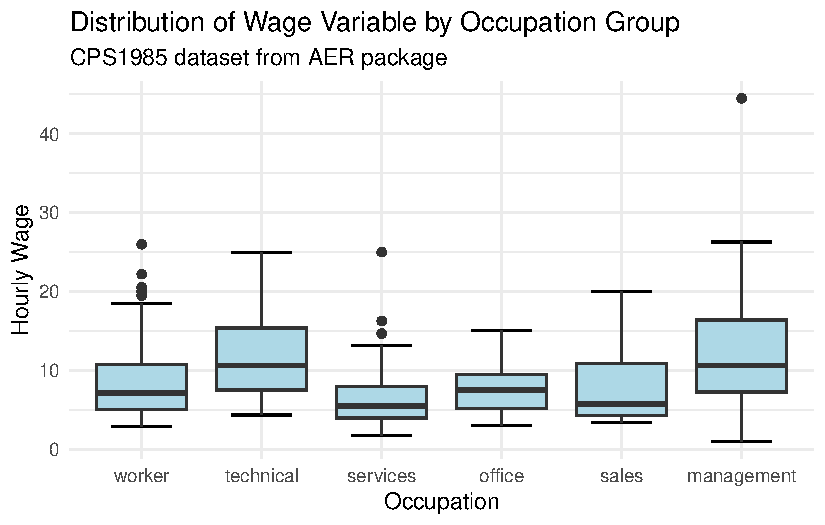
\includegraphics[keepaspectratio]{basicstats_files/figure-pdf/unnamed-chunk-23-1.pdf}}

The aesthetic of \texttt{aes(x\ =\ occupation,\ y\ =\ wage)} tells the
\texttt{ggplot()} that we are plotting wage on the y (vertical) axis and
occupation on the x (horizontal) axis. We can get more complicated with
our boxplots. Let's say we want to look at gender differences in the
distribution of wage.

\begin{Shaded}
\begin{Highlighting}[]
\NormalTok{CPS1985 }\SpecialCharTok{|\textgreater{}} 
  \FunctionTok{ggplot}\NormalTok{(}\FunctionTok{aes}\NormalTok{(}\AttributeTok{x =}\NormalTok{ gender, }\AttributeTok{y =}\NormalTok{ wage)) }\SpecialCharTok{+}
  \FunctionTok{stat\_boxplot}\NormalTok{(}\AttributeTok{geom =} \StringTok{"errorbar"}\NormalTok{, }\AttributeTok{width =} \FloatTok{0.5}\NormalTok{) }\SpecialCharTok{+}
  \FunctionTok{geom\_boxplot}\NormalTok{(}\AttributeTok{fill =} \StringTok{"lightblue"}\NormalTok{) }\SpecialCharTok{+}
  \FunctionTok{theme\_minimal}\NormalTok{() }\SpecialCharTok{+}
  \FunctionTok{labs}\NormalTok{(}\AttributeTok{title =} \StringTok{"Distribution of Wage Variable by Gender"}\NormalTok{,}
       \AttributeTok{subtitle =} \StringTok{"CPS1985 dataset from AER package"}\NormalTok{,}
       \AttributeTok{y =} \StringTok{"Hourly Wage"}\NormalTok{,}
       \AttributeTok{x =} \StringTok{""}\NormalTok{)}
\end{Highlighting}
\end{Shaded}

\pandocbounded{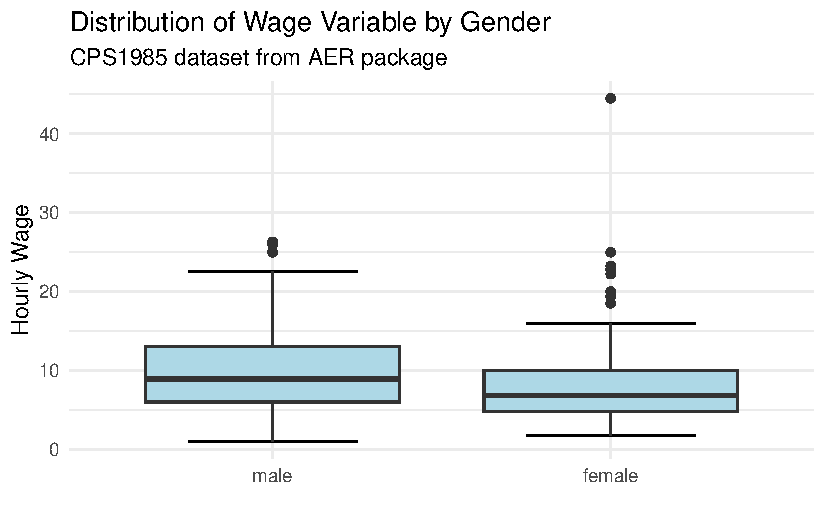
\includegraphics[keepaspectratio]{basicstats_files/figure-pdf/unnamed-chunk-24-1.pdf}}

Men seem to make more. Maybe your theory is that this gender wage gap is
driven by marital status, so now we have 2 factor variables. We can
include one of these factors as a fill aesthetic:

\begin{Shaded}
\begin{Highlighting}[]
\NormalTok{CPS1985 }\SpecialCharTok{|\textgreater{}} 
  \FunctionTok{ggplot}\NormalTok{(}\FunctionTok{aes}\NormalTok{(}\AttributeTok{x =}\NormalTok{ married, }\AttributeTok{y =}\NormalTok{ wage, }\AttributeTok{fill =}\NormalTok{ gender)) }\SpecialCharTok{+}
  \FunctionTok{geom\_boxplot}\NormalTok{() }\SpecialCharTok{+}
  \FunctionTok{theme\_minimal}\NormalTok{() }\SpecialCharTok{+}
  \FunctionTok{labs}\NormalTok{(}\AttributeTok{title =} \StringTok{"Distribution of Wage Variable by Gender and Marital Status"}\NormalTok{,}
       \AttributeTok{subtitle =} \StringTok{"CPS1985 dataset from AER package"}\NormalTok{,}
       \AttributeTok{y =} \StringTok{"Hourly Wage"}\NormalTok{,}
       \AttributeTok{x =} \StringTok{"Marital Status"}\NormalTok{,}
       \AttributeTok{fill =} \StringTok{"Gender"}\NormalTok{)}
\end{Highlighting}
\end{Shaded}

\pandocbounded{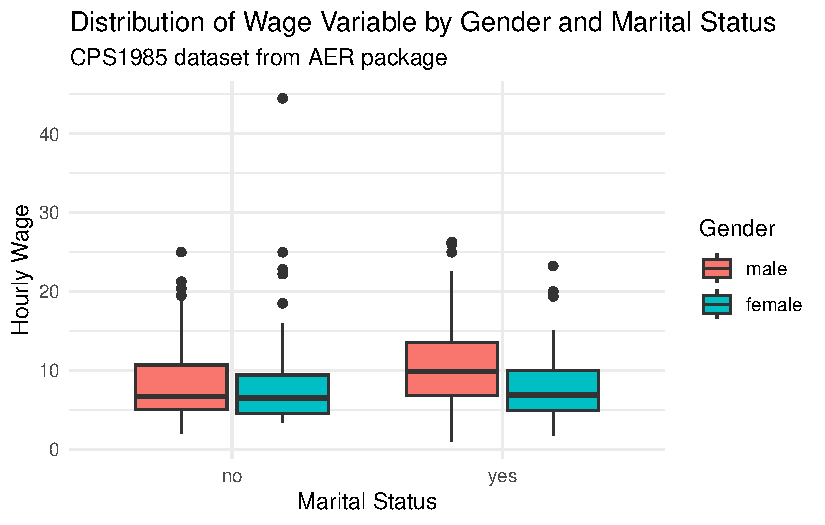
\includegraphics[keepaspectratio]{basicstats_files/figure-pdf/unnamed-chunk-25-1.pdf}}

A few things to note about the above code:

\begin{itemize}
\item
  I removed the \texttt{stat\_boxplot()} because it doesn't do a great
  job aligning itself with grouped boxes.
\item
  I eliminated the \texttt{fill} option in \texttt{geom\_boxplot}. Why?
  because I want the fill from the aesthetic to work! Right now, the
  genders have different colors for their boxplots. If I specified
  \texttt{fill} in the \texttt{geom\_boxplot()}, because it happens
  \emph{after} the \texttt{aes()}, the color coded genders will be
  overwritten!
\item
  Variables in the \texttt{aes()} that are \textbf{not} your x and y
  variables - variables like \texttt{fill}, \texttt{color},
  \texttt{size}, or \texttt{shape} - will automatically generate a
  legend. To name the legend, I added the \texttt{fill\ =\ "Gender"}
  line into the \texttt{labs()} function.
\end{itemize}

What happens if we put married as our fill variable and gender as our x
variable?

\begin{Shaded}
\begin{Highlighting}[]
\NormalTok{CPS1985 }\SpecialCharTok{|\textgreater{}} 
  \FunctionTok{ggplot}\NormalTok{(}\FunctionTok{aes}\NormalTok{(}\AttributeTok{x =}\NormalTok{ gender, }\AttributeTok{y =}\NormalTok{ wage, }\AttributeTok{fill =}\NormalTok{ married)) }\SpecialCharTok{+}
  \FunctionTok{geom\_boxplot}\NormalTok{() }\SpecialCharTok{+}
  \FunctionTok{theme\_minimal}\NormalTok{() }\SpecialCharTok{+}
  \FunctionTok{labs}\NormalTok{(}\AttributeTok{title =} \StringTok{"Distribution of Wage Variable by Gender and Marital Status"}\NormalTok{,}
       \AttributeTok{subtitle =} \StringTok{"CPS1985 dataset from AER package"}\NormalTok{,}
       \AttributeTok{y =} \StringTok{"Hourly Wage"}\NormalTok{,}
       \AttributeTok{fill =} \StringTok{"Marital Status"}\NormalTok{,}
       \AttributeTok{x =} \StringTok{"Gender"}\NormalTok{)}
\end{Highlighting}
\end{Shaded}

\pandocbounded{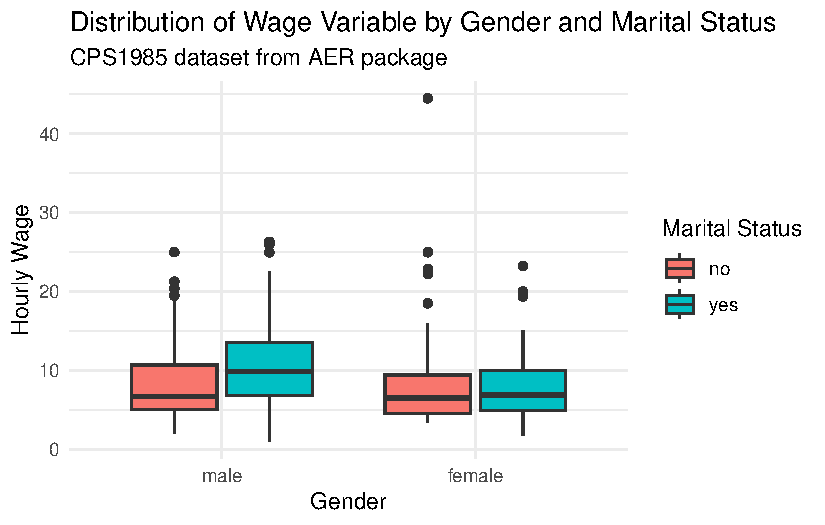
\includegraphics[keepaspectratio]{basicstats_files/figure-pdf/unnamed-chunk-26-1.pdf}}

Same data, same boxes, but the arrangement of the boxes tells a
different story.

Finally, for fun, let's consider taking this last graph and elevating it
a bit:

\begin{Shaded}
\begin{Highlighting}[]
\NormalTok{CPS1985 }\SpecialCharTok{|\textgreater{}} \FunctionTok{ggplot}\NormalTok{(}\FunctionTok{aes}\NormalTok{(}\AttributeTok{x =}\NormalTok{ married, }\AttributeTok{y =}\NormalTok{ wage, }\AttributeTok{fill =}\NormalTok{ gender)) }\SpecialCharTok{+}
    \FunctionTok{geom\_boxplot}\NormalTok{() }\SpecialCharTok{+}
    \FunctionTok{theme\_minimal}\NormalTok{() }\SpecialCharTok{+}
    \FunctionTok{labs}\NormalTok{(}\AttributeTok{title =} \StringTok{"Does Marriage Influence the Gender Wage Gap?"}\NormalTok{, }
         \AttributeTok{subtitle =} \StringTok{"1985 CPS data"}\NormalTok{,}
         \AttributeTok{x =} \StringTok{""}\NormalTok{, }
         \AttributeTok{y =} \StringTok{"Wages"}\NormalTok{,}
         \AttributeTok{fill =} \StringTok{""}\NormalTok{,}
         \AttributeTok{caption =} \StringTok{"@mattdobra"}\NormalTok{) }\SpecialCharTok{+}
    \FunctionTok{scale\_fill\_manual}\NormalTok{(}\AttributeTok{values=} \FunctionTok{c}\NormalTok{(}\StringTok{"deepskyblue4"}\NormalTok{, }\StringTok{"darksalmon"}\NormalTok{),}
                      \AttributeTok{labels =} \FunctionTok{c}\NormalTok{(}\StringTok{"male"} \OtherTok{=} \StringTok{"Male"}\NormalTok{, }\StringTok{"female"} \OtherTok{=} \StringTok{"Female"}\NormalTok{)) }\SpecialCharTok{+}
    \FunctionTok{theme}\NormalTok{(}\AttributeTok{legend.position =} \StringTok{"bottom"}\NormalTok{,}
          \AttributeTok{legend.direction =} \StringTok{"horizontal"}\NormalTok{) }\SpecialCharTok{+}
    \FunctionTok{scale\_x\_discrete}\NormalTok{(}\AttributeTok{labels =} \FunctionTok{c}\NormalTok{(}\StringTok{"no"} \OtherTok{=} \StringTok{"Unmarried"}\NormalTok{, }\StringTok{"yes"} \OtherTok{=} \StringTok{"Married"}\NormalTok{)) }
\end{Highlighting}
\end{Shaded}

\pandocbounded{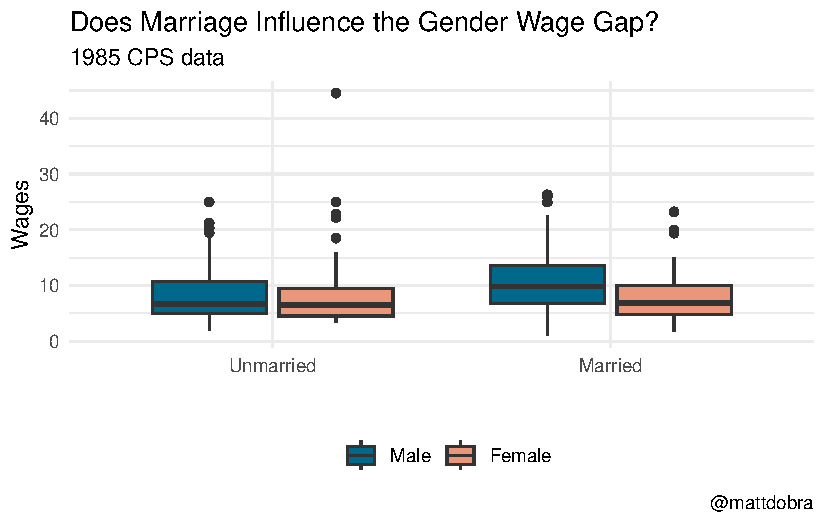
\includegraphics[keepaspectratio]{basicstats_files/figure-pdf/unnamed-chunk-27-1.pdf}}

Here's a quick breakdown of the changes I made:

\begin{itemize}
\item
  Visual and Aesthetic Changes:

  \begin{itemize}
  \item
    Custom colors: Replaced R's default red/teal with deepskyblue4 and
    darksalmon - a different take on blue/pink that's less jarring than
    stereotypical gender colors
  \item
    Legend positioning: Moved legend to bottom with horizontal
    orientation for cleaner layout
  \item
    Cleaner legend: Removed legend title (fill = ``\,``)
    since''Male/Female'' labels are self-explanatory
  \end{itemize}
\item
  Readability Improvements:

  \begin{itemize}
  \item
    More compelling title: Changed from descriptive ``Distribution
    of\ldots{}'' to research question ``Does Marriage Influence the
    Gender Wage Gap?''
  \item
    Better axis labels: ``Unmarried/Married'' instead of ``no/yes'' - no
    guessing required. This also allows me to remove the x-axis title
    entirely (\texttt{x\ =\ ""}) because the combination of our
    compelling graph title and self-explanatory axis labels means
    readers don't need that extra layer of explanation.
  \item
    Capitalized legend labels: ``Male/Female'' instead of lowercase
    variable values
  \item
    Added subtitle and caption: Context and attribution
  \end{itemize}
\end{itemize}

\subsection{Histograms}\label{histograms}

Like \hyperref[boxplots]{Boxplots}, histograms are useful for displaying
the distribution of continuous data. Also like
\hyperref[boxplots]{Boxplots}, these are much easier to create in R than
in Excel! Since histograms and boxplots have similar vibes, let's
continue to look at the distribution of respondent income in the CPS1985
data set so you can think about which works better for this data.

\begin{Shaded}
\begin{Highlighting}[]
\NormalTok{CPS1985 }\SpecialCharTok{|\textgreater{}} \FunctionTok{ggplot}\NormalTok{(}\FunctionTok{aes}\NormalTok{(}\AttributeTok{x =}\NormalTok{ wage)) }\SpecialCharTok{+}
    \FunctionTok{geom\_histogram}\NormalTok{()}
\end{Highlighting}
\end{Shaded}

\begin{verbatim}
`stat_bin()` using `bins = 30`. Pick better value with `binwidth`.
\end{verbatim}

\pandocbounded{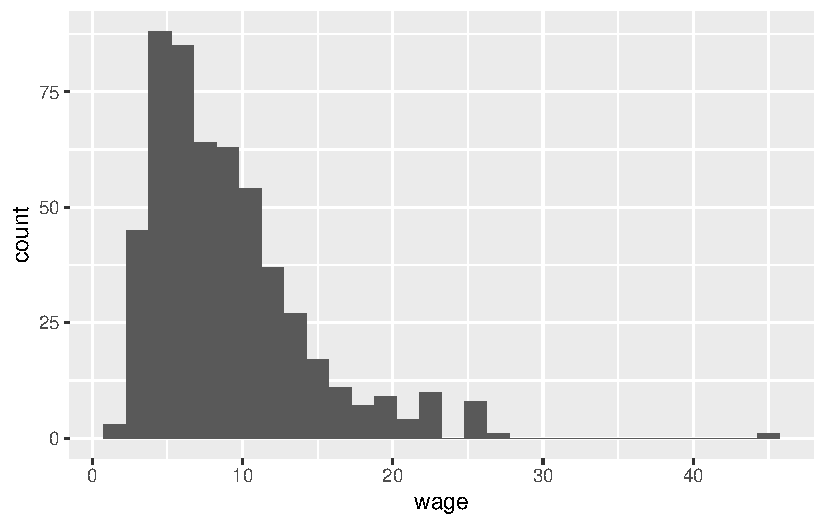
\includegraphics[keepaspectratio]{basicstats_files/figure-pdf/unnamed-chunk-28-1.pdf}}

As you can see, we got a message telling us that
\texttt{geom\_histogram()} defaults to 30 bins, and the implied critism
is that perhaps 30 is not the right number of bins for your data! This
is generally a true statement, by the way, the right answer is probably
not to stick with the defaults. We have options for fixing this:

\begin{itemize}
\tightlist
\item
  Change the width of the bins with \texttt{binwidth\ =}
\item
  Set the number of bins explicitly with \texttt{bins\ =}
\item
  Look the other way, set \texttt{\#\textbar{}\ message:\ false} in the
  YAML so the message doesn't pop up anymore, and move on with our
  lives. YOLO!
\end{itemize}

\begin{center}

\includegraphics[width=0.75\linewidth,height=\textheight,keepaspectratio]{images/nothingtosee.jpg}
\end{center}

Choosing bins is equal parts art and science, and the authoritative
``rules'' for it aren't always up to the task when it comes to real
world data, especially data describing human behavior. I've never
particularly liked any treatment I've seen for choosing it in intro
stats texts. So I'll share with you my general method for choosing bins:

\begin{enumerate}
\def\labelenumi{\arabic{enumi}.}
\tightlist
\item
  Start with the \(\sqrt{n}\). This gives a rough approximation of how
  many bins I should have.
\item
  Identify the range of the data, ignoring outliers, you probably want
  something like the 2nd percentile and the 98th percentile. Divide the
  range by the \(\sqrt{n}\), this gives you a rough idea of what the
  right binwidth should be.
\item
  Identify round numbers and natural breakpoints to ensure the data
  isn't going to be too ``lumpy.'' No, that's not a technical term. I'll
  explain more when I give an example!
\item
  Set binwidths based on the first three guidelines.
\item
  Don't be afraid to ignore the first 4 rules if needed.
\end{enumerate}

So, for this case, we start with step 1 and note that the dataset
includes 534 observations, and \(\sqrt{534} \approx 23.11\). For step 2,
our 2nd and 98th percentile values are \$3.35 and \$22.97, so a
\texttt{binwidth} of around \$0.84 is a good starting point. But now for
step 3: using binwidths of \$0.84 might create problems as real world
hourly wages are far more likely to be \$8.00 or \$9.00 than \$8.01 or
\$8.99, because humans like round numbers. And if we had bins of \$0.84
or whatever, we might wind up with a bin from \$8.03 to \$8.87 and it
would look arbitrarily small compared to the bin that preceded it and
the bin that came after it - not because wages are multimodal or
something but just because of the lumpiness of the underlying numbers.
So we probably want to instead think about using round numbers for our
bins, so we are now thinking about intervals of \$1.00. So we will start
there, but also consider maybe bigger numbers (binwidths of maybe \$1.50
or \$2.00) if it creates a smoother graph. But not too smooth\ldots like
I said, art and science.

To see what this all looks like in action, let's start with a graph that
has the \texttt{binwidth} set way too low with
\texttt{binwidth\ =\ 0.42}. Here, you can imagine bins like \$7.52 to
\$7.94 that will contain very few people with those wages, meanwhile the
bins in which round numbers fall like \$7.00 or \$8.00 will look like
spikes in the graph.

\begin{Shaded}
\begin{Highlighting}[]
\NormalTok{CPS1985 }\SpecialCharTok{|\textgreater{}} \FunctionTok{ggplot}\NormalTok{(}\FunctionTok{aes}\NormalTok{(}\AttributeTok{x =}\NormalTok{ wage)) }\SpecialCharTok{+}
    \FunctionTok{geom\_histogram}\NormalTok{(}\AttributeTok{binwidth =} \FloatTok{0.42}\NormalTok{) }\SpecialCharTok{+}
    \FunctionTok{theme\_minimal}\NormalTok{() }\SpecialCharTok{+}
    \FunctionTok{labs}\NormalTok{(}\AttributeTok{title =} \StringTok{"Binwidth = 0.42"}\NormalTok{)}
\end{Highlighting}
\end{Shaded}

\begin{figure}[H]

{\centering \pandocbounded{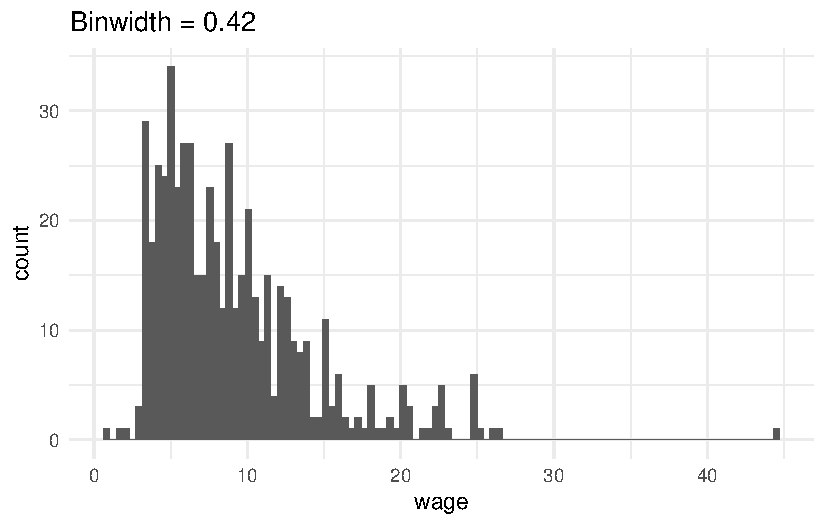
\includegraphics[keepaspectratio]{basicstats_files/figure-pdf/unnamed-chunk-30-1.pdf}}

}

\caption{Binwidth = 0.42 (Super Lumpy)}

\end{figure}%

The human tendency to like round numbers makes the data lumpy, and
choosing too small bins makes the histogram spiky (also not a technical
term). By the way, here is a list the wages in the dataset that appear
at least 10 times:

\begin{longtable}[]{@{}rr@{}}
\toprule\noalign{}
Hourly Wage & Count \\
\midrule\noalign{}
\endhead
\bottomrule\noalign{}
\endlastfoot
5.00 & 18 \\
10.00 & 18 \\
7.50 & 14 \\
6.25 & 12 \\
7.00 & 12 \\
4.50 & 12 \\
3.35 & 12 \\
5.50 & 12 \\
8.00 & 11 \\
6.00 & 11 \\
4.00 & 10 \\
12.00 & 10 \\
15.00 & 10 \\
3.50 & 10 \\
\end{longtable}

Notice a pattern? The two most common are multiples of \$5.00, then you
have \$7.50 (the halfway point between \$5.00 and \$10.00), and then
\$6.25 (the halfway point between \$5.00 and \$7.50). Over half of the
entries are round numbers, and all but one are multiples of 0.25. The
outlier, \$3.35? That's the minimum wage in 1985!

Data generated by human processes or about humans are notorious for this
sort of lumpiness. And money is inherently lumpy, I guess, but think
about something that is not. Human height. It's probably the case that
the number of men in the world who are 72'' tall (6 feet) is roughly the
same as the number who are 71.9'' tall or 72.1'' tall, but who the heck
says they are 72.1'' tall? Nobody! And from what I can tell, most people
who are 70'' tall round up to 6 foot anyway\ldots look guys, I'm a legit
6'2'', I can see what you are doing from up here.

Moving on to the two mentioned above, the next two graphs set binwidths
of \$0.84 and \$1.00, respectively:

\begin{Shaded}
\begin{Highlighting}[]
\CommentTok{\# Mathematical approach}
\NormalTok{CPS1985 }\SpecialCharTok{|\textgreater{}} \FunctionTok{ggplot}\NormalTok{(}\FunctionTok{aes}\NormalTok{(}\AttributeTok{x =}\NormalTok{ wage)) }\SpecialCharTok{+}
    \FunctionTok{geom\_histogram}\NormalTok{(}\AttributeTok{binwidth =} \FloatTok{0.84}\NormalTok{) }\SpecialCharTok{+}
    \FunctionTok{theme\_minimal}\NormalTok{() }\SpecialCharTok{+}
    \FunctionTok{labs}\NormalTok{(}\AttributeTok{title =} \StringTok{"Binwidth = 0.84"}\NormalTok{)}
\CommentTok{\# Round number approach  }
\NormalTok{CPS1985 }\SpecialCharTok{|\textgreater{}} \FunctionTok{ggplot}\NormalTok{(}\FunctionTok{aes}\NormalTok{(}\AttributeTok{x =}\NormalTok{ wage)) }\SpecialCharTok{+}
    \FunctionTok{geom\_histogram}\NormalTok{(}\AttributeTok{binwidth =} \DecValTok{1}\NormalTok{) }\SpecialCharTok{+}
    \FunctionTok{theme\_minimal}\NormalTok{() }\SpecialCharTok{+}
    \FunctionTok{labs}\NormalTok{(}\AttributeTok{title =} \StringTok{"Binwidth = 1"}\NormalTok{)}
\end{Highlighting}
\end{Shaded}

\begin{figure}

\begin{minipage}{0.50\linewidth}

\begin{figure}[H]

{\centering \pandocbounded{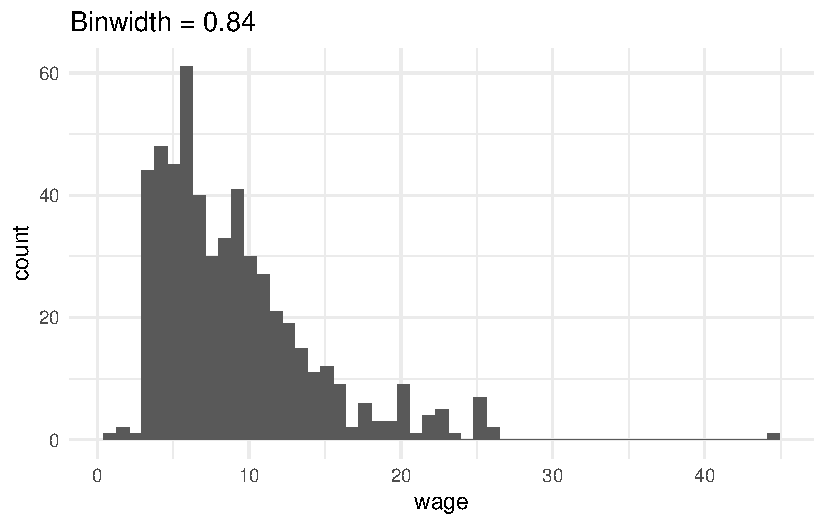
\includegraphics[keepaspectratio]{basicstats_files/figure-pdf/unnamed-chunk-32-1.pdf}}

}

\subcaption{Binwidth = 0.84 (Mathematical)}

\end{figure}%

\end{minipage}%
%
\begin{minipage}{0.50\linewidth}

\begin{figure}[H]

{\centering \pandocbounded{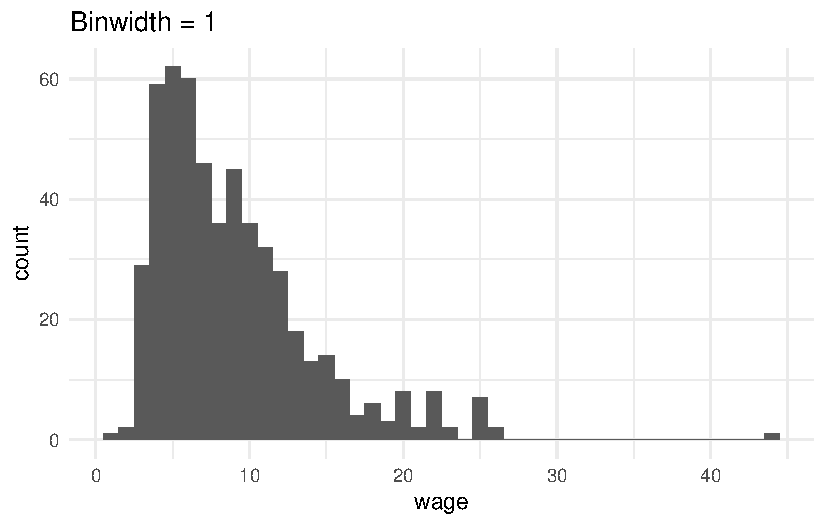
\includegraphics[keepaspectratio]{basicstats_files/figure-pdf/unnamed-chunk-32-2.pdf}}

}

\subcaption{Binwidth = 1 (Practical)}

\end{figure}%

\end{minipage}%

\end{figure}%

While not as pronounced as the \texttt{binwidth\ =\ 0.42} version, the
\texttt{binwidth\ =\ 0.84} graph is indeed a little spikier than using
\texttt{binwidth\ =\ 1}, I think I'd prefer the latter. We might even
consider bigger binwidths to see what they look like; here are binwidths
of \$1.50 and \$2.00:

\begin{Shaded}
\begin{Highlighting}[]
\NormalTok{CPS1985 }\SpecialCharTok{|\textgreater{}} \FunctionTok{ggplot}\NormalTok{(}\FunctionTok{aes}\NormalTok{(}\AttributeTok{x =}\NormalTok{ wage)) }\SpecialCharTok{+}
    \FunctionTok{geom\_histogram}\NormalTok{(}\AttributeTok{binwidth =} \FloatTok{1.5}\NormalTok{) }\SpecialCharTok{+}
    \FunctionTok{theme\_minimal}\NormalTok{() }\SpecialCharTok{+}
    \FunctionTok{labs}\NormalTok{(}\AttributeTok{title =} \StringTok{"Binwidth = 1.5"}\NormalTok{)}
\NormalTok{CPS1985 }\SpecialCharTok{|\textgreater{}} \FunctionTok{ggplot}\NormalTok{(}\FunctionTok{aes}\NormalTok{(}\AttributeTok{x =}\NormalTok{ wage)) }\SpecialCharTok{+}
    \FunctionTok{geom\_histogram}\NormalTok{(}\AttributeTok{binwidth =} \DecValTok{2}\NormalTok{) }\SpecialCharTok{+}
    \FunctionTok{theme\_minimal}\NormalTok{() }\SpecialCharTok{+}
    \FunctionTok{labs}\NormalTok{(}\AttributeTok{title =} \StringTok{"Binwidth = 2"}\NormalTok{)}
\end{Highlighting}
\end{Shaded}

\begin{figure}

\begin{minipage}{0.50\linewidth}

\begin{figure}[H]

{\centering \pandocbounded{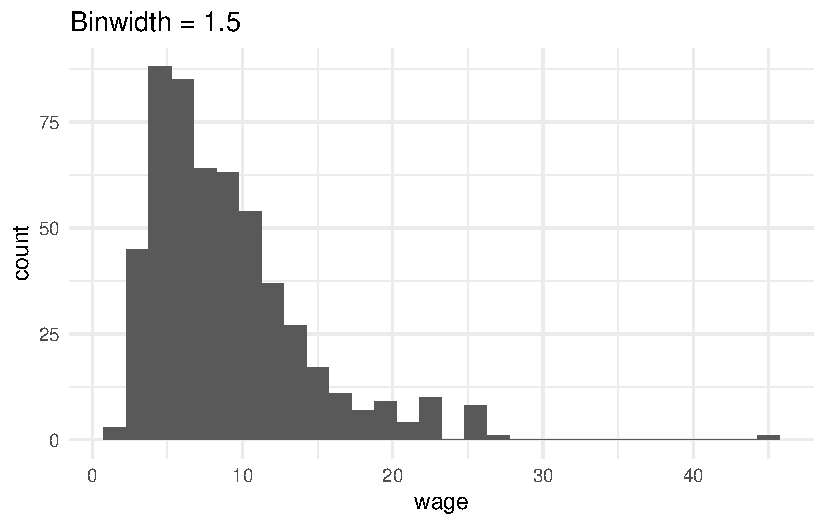
\includegraphics[keepaspectratio]{basicstats_files/figure-pdf/unnamed-chunk-33-1.pdf}}

}

\subcaption{Binwidth = 1.5 (Smoother)}

\end{figure}%

\end{minipage}%
%
\begin{minipage}{0.50\linewidth}

\begin{figure}[H]

{\centering \pandocbounded{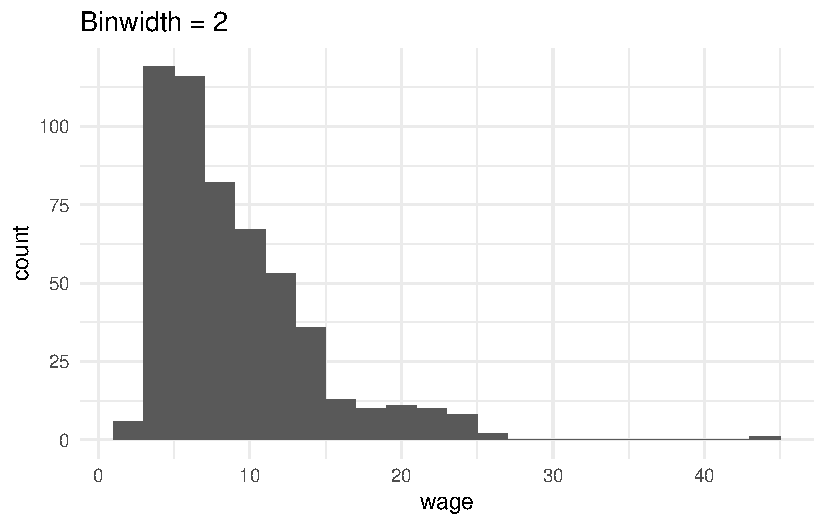
\includegraphics[keepaspectratio]{basicstats_files/figure-pdf/unnamed-chunk-33-2.pdf}}

}

\subcaption{Binwidth = 2 (Very Smooth)}

\end{figure}%

\end{minipage}%

\end{figure}%

Now we are getting to the point that we are eliminating a lot of the
artifacts that are creating the artificial lumpiness in the data, but at
a cost of losing precision. I'll say it again, art and science. I think
either the \$1.00 or \$\$2.00 graph work the best for me, so let's go
ahead and clean up the \$2.00 by setting some common options that are
typical when using \texttt{geom\_histogram()}:

\begin{Shaded}
\begin{Highlighting}[]
\NormalTok{CPS1985 }\SpecialCharTok{|\textgreater{}} \FunctionTok{ggplot}\NormalTok{(}\FunctionTok{aes}\NormalTok{(}\AttributeTok{x =}\NormalTok{ wage)) }\SpecialCharTok{+}
  \FunctionTok{geom\_histogram}\NormalTok{(}\AttributeTok{binwidth =} \DecValTok{2}\NormalTok{,}
                 \AttributeTok{fill =} \StringTok{"lightsteelblue"}\NormalTok{,}
                 \AttributeTok{color =} \StringTok{"steelblue"}\NormalTok{) }\SpecialCharTok{+}
  \FunctionTok{theme\_minimal}\NormalTok{() }\SpecialCharTok{+}  
  \FunctionTok{theme}\NormalTok{(}\AttributeTok{panel.grid.major.x =} \FunctionTok{element\_blank}\NormalTok{(),}
        \AttributeTok{panel.grid.minor.x =} \FunctionTok{element\_blank}\NormalTok{()) }\SpecialCharTok{+}
  \FunctionTok{scale\_x\_continuous}\NormalTok{(}\AttributeTok{expand =} \FunctionTok{c}\NormalTok{(}\DecValTok{0}\NormalTok{, }\DecValTok{0}\NormalTok{)) }\SpecialCharTok{+}
  \FunctionTok{scale\_y\_continuous}\NormalTok{(}\AttributeTok{expand =} \FunctionTok{c}\NormalTok{(}\DecValTok{0}\NormalTok{, }\DecValTok{0}\NormalTok{)) }\SpecialCharTok{+}
  \FunctionTok{labs}\NormalTok{(}\AttributeTok{title =} \StringTok{"Distribution of Wages"}\NormalTok{,}
       \AttributeTok{subtitle =} \StringTok{"Data from 1985 CPS"}\NormalTok{,}
       \AttributeTok{caption =} \StringTok{"Sample Size: 534"}\NormalTok{,}
       \AttributeTok{y =} \StringTok{"Count"}\NormalTok{,}
       \AttributeTok{x =} \StringTok{"Hourly Wage"}\NormalTok{)}
\end{Highlighting}
\end{Shaded}

\begin{figure}[H]

{\centering \pandocbounded{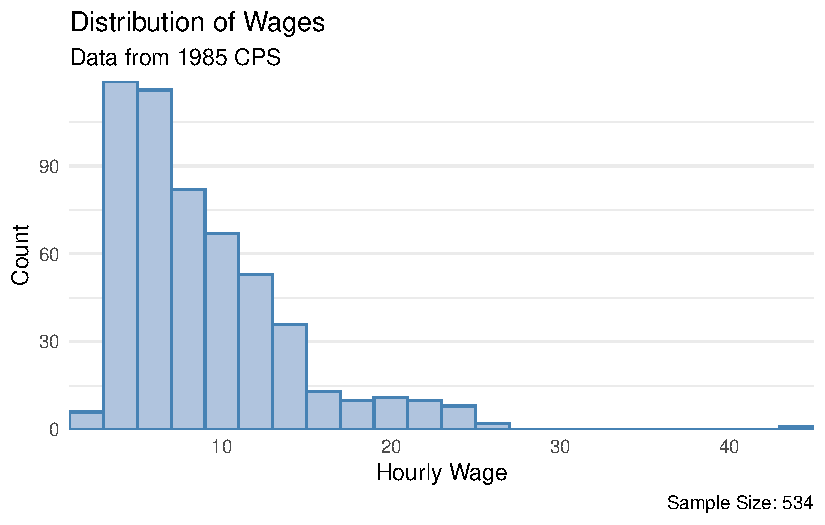
\includegraphics[keepaspectratio]{basicstats_files/figure-pdf/unnamed-chunk-34-1.pdf}}

}

\caption{Histogram}

\end{figure}%

Just a few finishing touches make this histogram much more polished:

\begin{itemize}
\tightlist
\item
  Custom colors: The \texttt{fill} and \texttt{color} options give us a
  cohesive blue theme instead of the default gray. Remember,
  \texttt{color} is for points and lines (0 and 1 dimensional objects)
  while \texttt{fill} is for areas (2 dimensional spaces)
\item
  Cleaner gridlines: Removing vertical gridlines with \texttt{theme()}
  since they're not particularly helpful for histograms
\item
  Tighter spacing: \texttt{expand\ =\ c(0,0)} eliminates the awkward
  white space between the axes and the data
\item
  Complete labeling: Title, subtitle, and caption provide context, and
  capitalizing ``Count'' is cleaner than the default ``count''
\end{itemize}

\subsection{Stacked and Grouped Bar Charts (and Pie Charts I
Guess)}\label{stacked-and-grouped-bar-charts-and-pie-charts-i-guess}

Stacked and Grouped Bar Charts are typically used to look at
compositions of groups\ldots that is to say, groups within groups. First
you group, then you subgroup. This is a pretty simple augmentation to
the \texttt{geom\_bar()} from above, where all we need to do is set both
an \texttt{x} variable for our groups, and a \texttt{fill} variable for
our subgroups within our groups. This looks at the distribution of
genders within each occupation class in the \texttt{CPS1985} data:

\begin{Shaded}
\begin{Highlighting}[]
\NormalTok{CPS1985 }\SpecialCharTok{|\textgreater{}} 
  \FunctionTok{ggplot}\NormalTok{(}\FunctionTok{aes}\NormalTok{(}\AttributeTok{x =}\NormalTok{ occupation, }\AttributeTok{fill =}\NormalTok{ gender)) }\SpecialCharTok{+}
  \FunctionTok{geom\_bar}\NormalTok{() }
\end{Highlighting}
\end{Shaded}

\pandocbounded{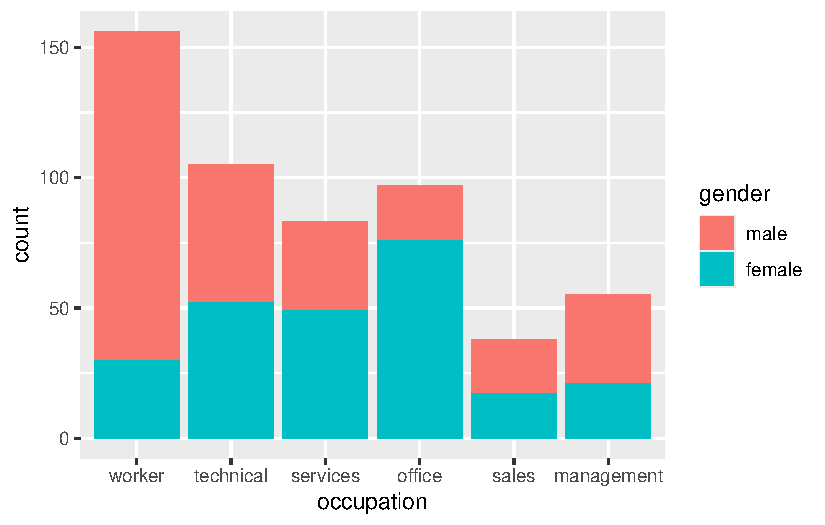
\includegraphics[keepaspectratio]{basicstats_files/figure-pdf/unnamed-chunk-35-1.pdf}}

Let's clean this up and definitely edit the colors. Gender stereotype
colors (i.e.~blue for men, pink for women) probably enhance readability
to the viewer, but if you want to avoid them, then you probably don't
want to do the exact opposite of what people expect! We'll stick with
our blue/salmon combo that's less jarring but still provides good
contrast. Plus, nothing is easier than doing a copy/paste on the
\texttt{scale\_fill\_manual()} line from a few graphs back that we
\emph{know} works, as well as give this chart some labels:

\begin{Shaded}
\begin{Highlighting}[]
\NormalTok{CPS1985 }\SpecialCharTok{|\textgreater{}} 
  \FunctionTok{ggplot}\NormalTok{(}\FunctionTok{aes}\NormalTok{(}\AttributeTok{x =}\NormalTok{ occupation, }\AttributeTok{fill =}\NormalTok{ gender)) }\SpecialCharTok{+}
  \FunctionTok{geom\_bar}\NormalTok{() }\SpecialCharTok{+}
  \FunctionTok{theme\_minimal}\NormalTok{() }\SpecialCharTok{+}
  \FunctionTok{scale\_fill\_manual}\NormalTok{(}\AttributeTok{values=} \FunctionTok{c}\NormalTok{(}\StringTok{"deepskyblue4"}\NormalTok{, }\StringTok{"darksalmon"}\NormalTok{),}
                    \AttributeTok{labels =} \FunctionTok{c}\NormalTok{(}\StringTok{"male"} \OtherTok{=} \StringTok{"Male"}\NormalTok{, }\StringTok{"female"} \OtherTok{=} \StringTok{"Female"}\NormalTok{)) }\SpecialCharTok{+}
  \FunctionTok{labs}\NormalTok{(}\AttributeTok{x =} \StringTok{"Occupation"}\NormalTok{,}
       \AttributeTok{y =} \StringTok{"Count"}\NormalTok{,}
       \AttributeTok{fill =} \StringTok{"Gender"}\NormalTok{,}
       \AttributeTok{title =} \StringTok{"Distribution of Gender by Occupation"}\NormalTok{)}
\end{Highlighting}
\end{Shaded}

\pandocbounded{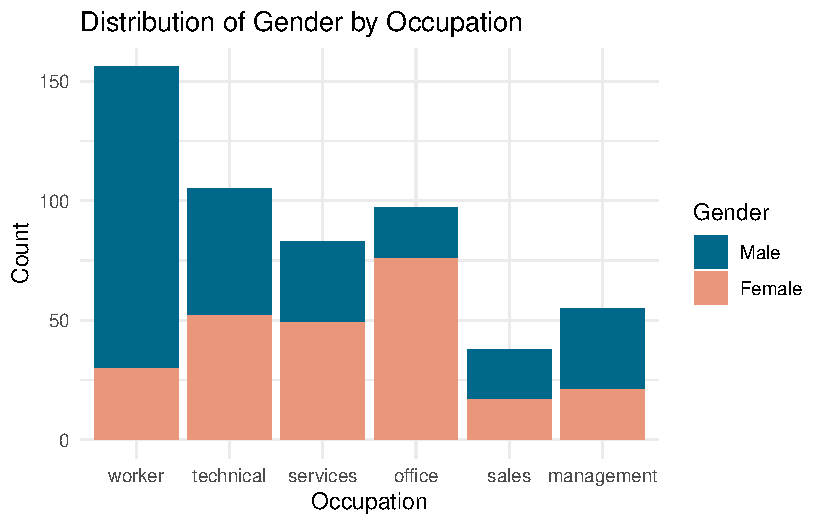
\includegraphics[keepaspectratio]{basicstats_files/figure-pdf/unnamed-chunk-36-1.pdf}}

Rather than stacking the bars, we can create side-by-side bars by adding
the \texttt{position\ =\ "dodge"} option in the \texttt{geom\_bar()}
layer.

\begin{Shaded}
\begin{Highlighting}[]
\NormalTok{CPS1985 }\SpecialCharTok{|\textgreater{}} 
  \FunctionTok{ggplot}\NormalTok{(}\FunctionTok{aes}\NormalTok{(}\AttributeTok{x =}\NormalTok{ occupation, }\AttributeTok{fill =}\NormalTok{ gender)) }\SpecialCharTok{+}
  \FunctionTok{geom\_bar}\NormalTok{(}\AttributeTok{position =} \StringTok{"dodge"}\NormalTok{) }\SpecialCharTok{+}
  \FunctionTok{theme\_minimal}\NormalTok{() }\SpecialCharTok{+}
  \FunctionTok{scale\_fill\_manual}\NormalTok{(}\AttributeTok{values=} \FunctionTok{c}\NormalTok{(}\StringTok{"deepskyblue4"}\NormalTok{, }\StringTok{"darksalmon"}\NormalTok{),}
                    \AttributeTok{labels =} \FunctionTok{c}\NormalTok{(}\StringTok{"male"} \OtherTok{=} \StringTok{"Male"}\NormalTok{, }\StringTok{"female"} \OtherTok{=} \StringTok{"Female"}\NormalTok{)) }\SpecialCharTok{+}
  \FunctionTok{labs}\NormalTok{(}\AttributeTok{x =} \StringTok{"Occupation"}\NormalTok{,}
       \AttributeTok{y =} \StringTok{"Count"}\NormalTok{,}
       \AttributeTok{fill =} \StringTok{"Gender"}\NormalTok{,}
       \AttributeTok{title =} \StringTok{"Distribution of Gender by Occupation"}\NormalTok{)}
\end{Highlighting}
\end{Shaded}

\pandocbounded{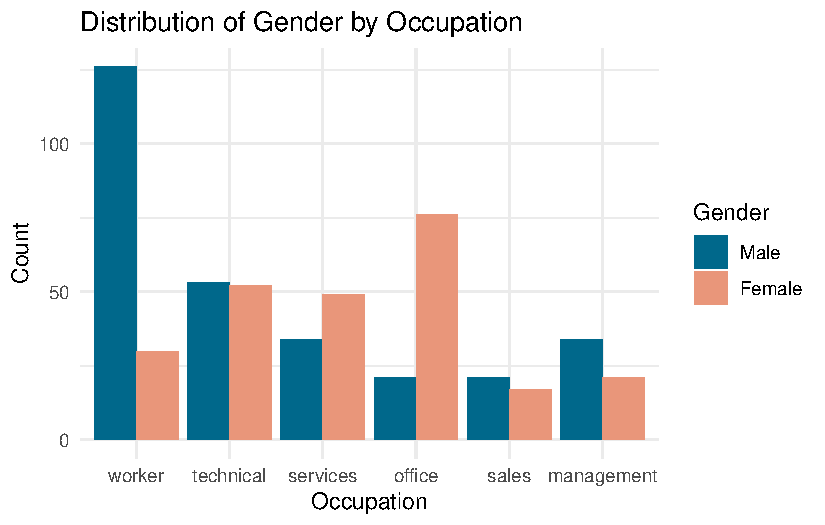
\includegraphics[keepaspectratio]{basicstats_files/figure-pdf/unnamed-chunk-37-1.pdf}}

A common use of the stacked bar chart is to compare subgroup proportions
between groups. For example, in the graphs above, we can see that there
are more people in the technical category than in sales, but it's harder
to compare the relative gender percentages across occupations. Is the
percentage of men in technical higher or lower than in sales? And by how
much? To accomplish this, we use the \texttt{position\ =\ "fill"} option
in our \texttt{geom\_bar()} layer.

\begin{Shaded}
\begin{Highlighting}[]
\NormalTok{CPS1985 }\SpecialCharTok{|\textgreater{}} 
  \FunctionTok{ggplot}\NormalTok{(}\FunctionTok{aes}\NormalTok{(}\AttributeTok{x =}\NormalTok{ occupation, }\AttributeTok{fill =}\NormalTok{ gender)) }\SpecialCharTok{+}
  \FunctionTok{geom\_bar}\NormalTok{(}\AttributeTok{position =} \StringTok{"fill"}\NormalTok{) }\SpecialCharTok{+}
  \FunctionTok{theme\_minimal}\NormalTok{() }\SpecialCharTok{+}
  \FunctionTok{scale\_fill\_manual}\NormalTok{(}\AttributeTok{values=} \FunctionTok{c}\NormalTok{(}\StringTok{"deepskyblue4"}\NormalTok{, }\StringTok{"darksalmon"}\NormalTok{),}
                    \AttributeTok{labels =} \FunctionTok{c}\NormalTok{(}\StringTok{"male"} \OtherTok{=} \StringTok{"Male"}\NormalTok{, }\StringTok{"female"} \OtherTok{=} \StringTok{"Female"}\NormalTok{)) }\SpecialCharTok{+}
  \FunctionTok{labs}\NormalTok{(}\AttributeTok{x =} \StringTok{"Occupation"}\NormalTok{,}
       \AttributeTok{y =} \StringTok{"Share"}\NormalTok{,}
       \AttributeTok{fill =} \StringTok{"Gender"}\NormalTok{,}
       \AttributeTok{title =} \StringTok{"Distribution of Gender by Occupation"}\NormalTok{)}
\end{Highlighting}
\end{Shaded}

\pandocbounded{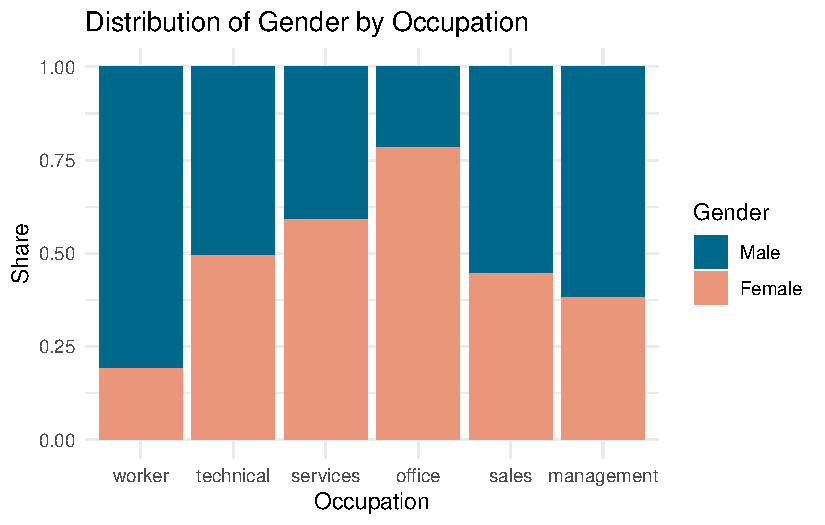
\includegraphics[keepaspectratio]{basicstats_files/figure-pdf/unnamed-chunk-38-1.pdf}}

This version of the stacked bar chart makes it easier to compare
subgroup proportions across groups.

\subsubsection{Pie Charts}\label{pie-charts}

And we are back at pie charts. I kindly ask that you refer back to my
Padme/Anakin meme (Figure~\ref{fig-padme-anakin}) from above before
continuing to read.

Most people's default understanding of a pie chart is as a circle that
is used to represent proportions; the circle is divided into wedges of
various sizes, where each wedge represents a group, and the size of each
wedge indicates the proportion of the whole that group makes up. This is
all well and good, but to make a pie chart in \texttt{ggplot()}, we need
to develop a different intuition: a pie chart is a stacked bar chart
that you have forced to be round.

To see what I mean, let's start with a simple stacked bar chart of the
occupation data. The code is fairly straightforward, the only oddity
here is the use of the \texttt{y\ =\ ""} in the \texttt{aes()} argument.
The effect of this is to simply select the entire dataset. Setting the
width of the \texttt{geom\_bar()} is not necessary, it just aids in my
being able to place a visual cue in the next graph. I'm also using the
\texttt{viridis} color scheme to aid with graph visibility.

\begin{Shaded}
\begin{Highlighting}[]
\NormalTok{CPS1985 }\SpecialCharTok{|\textgreater{}}  
  \FunctionTok{ggplot}\NormalTok{(}\FunctionTok{aes}\NormalTok{(}\AttributeTok{y =} \StringTok{""}\NormalTok{, }\AttributeTok{fill =}\NormalTok{ occupation)) }\SpecialCharTok{+}
  \FunctionTok{geom\_bar}\NormalTok{(}\AttributeTok{width =} \FloatTok{0.5}\NormalTok{) }\SpecialCharTok{+}
  \FunctionTok{scale\_fill\_viridis\_d}\NormalTok{() }
\end{Highlighting}
\end{Shaded}

\pandocbounded{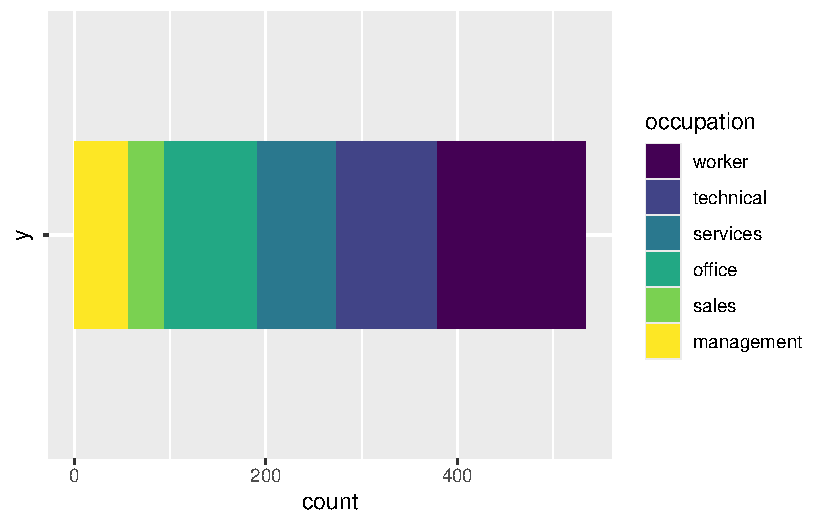
\includegraphics[keepaspectratio]{basicstats_files/figure-pdf/unnamed-chunk-39-1.pdf}}

Behold this horizontal stripe of rainbowy goodness! Next, let's place a
reference dot along the top of the bar, exactly in the middle of the x
dimension. I've done this below with the \texttt{geom\_point()} layer. :

\begin{Shaded}
\begin{Highlighting}[]
\NormalTok{CPS1985 }\SpecialCharTok{|\textgreater{}} 
  \FunctionTok{ggplot}\NormalTok{(}\FunctionTok{aes}\NormalTok{(}\AttributeTok{y =} \StringTok{""}\NormalTok{, }\AttributeTok{fill =}\NormalTok{ occupation)) }\SpecialCharTok{+}
  \FunctionTok{geom\_bar}\NormalTok{(}\AttributeTok{width =} \FloatTok{0.5}\NormalTok{) }\SpecialCharTok{+}
  \FunctionTok{scale\_fill\_viridis\_d}\NormalTok{() }\SpecialCharTok{+}
  \FunctionTok{geom\_point}\NormalTok{(}\AttributeTok{y =} \FloatTok{1.25}\NormalTok{, }\AttributeTok{x =} \DecValTok{267}\NormalTok{, }\AttributeTok{size =} \FloatTok{2.2}\NormalTok{, }\AttributeTok{show.legend =} \ConstantTok{FALSE}\NormalTok{)}
\end{Highlighting}
\end{Shaded}

\pandocbounded{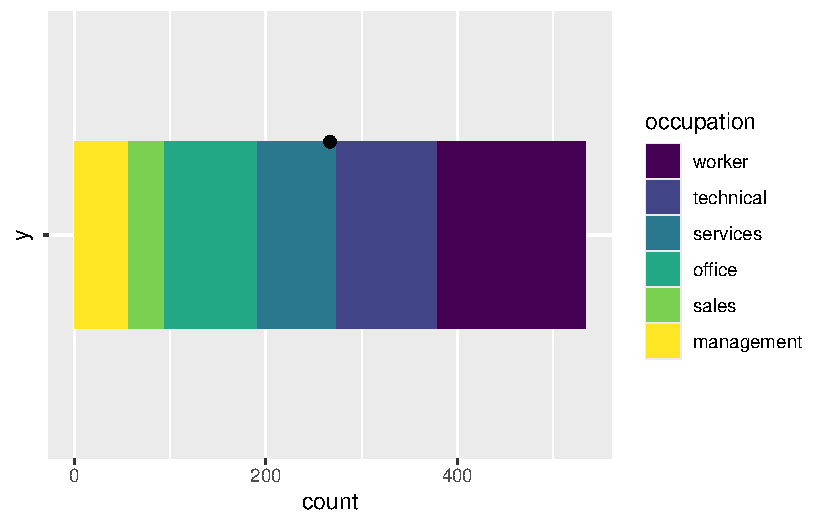
\includegraphics[keepaspectratio]{basicstats_files/figure-pdf/unnamed-chunk-40-1.pdf}}

Now, imagine what would happen if you took this shape and started
bending the two ends upward, using the black dot as a pivot point. This
will cause the top edge to shrink and the bottom edge to stretch. Keep
bending this shape around that pivot point until the top edge has shrunk
to a single point, the bottom edge has created a circle that completely
surrounds the black dot, and the two ends connect, so the far left
yellow edge is now flush with the far right purple edge. Break the
spirit of the noble stacked bar chart, and literally bend it to your
will! Now you have a pie chart!

\begin{center}

\includegraphics[width=0.5\linewidth,height=\textheight,keepaspectratio]{images/piecharts.jpg}
\end{center}

More mathily, we can say that we converted your cartesian coordinate
system (the standard \((x,y)\) space you learned in high school algebra)
into a polar coordinate system. So we take the stacked bar from above,
and add one line of code: \texttt{coord\_polar(theta\ =\ "x")}. And
that's all it takes, we have a pie chart:

\begin{Shaded}
\begin{Highlighting}[]
\NormalTok{CPS1985 }\SpecialCharTok{|\textgreater{}} 
  \FunctionTok{ggplot}\NormalTok{(}\FunctionTok{aes}\NormalTok{(}\AttributeTok{y =} \StringTok{""}\NormalTok{, }\AttributeTok{fill =}\NormalTok{ occupation)) }\SpecialCharTok{+}
  \FunctionTok{geom\_bar}\NormalTok{(}\AttributeTok{width =} \FloatTok{0.5}\NormalTok{) }\SpecialCharTok{+}
  \FunctionTok{scale\_fill\_viridis\_d}\NormalTok{() }\SpecialCharTok{+}
  \FunctionTok{coord\_polar}\NormalTok{(}\AttributeTok{theta =} \StringTok{"x"}\NormalTok{)}
\end{Highlighting}
\end{Shaded}

\pandocbounded{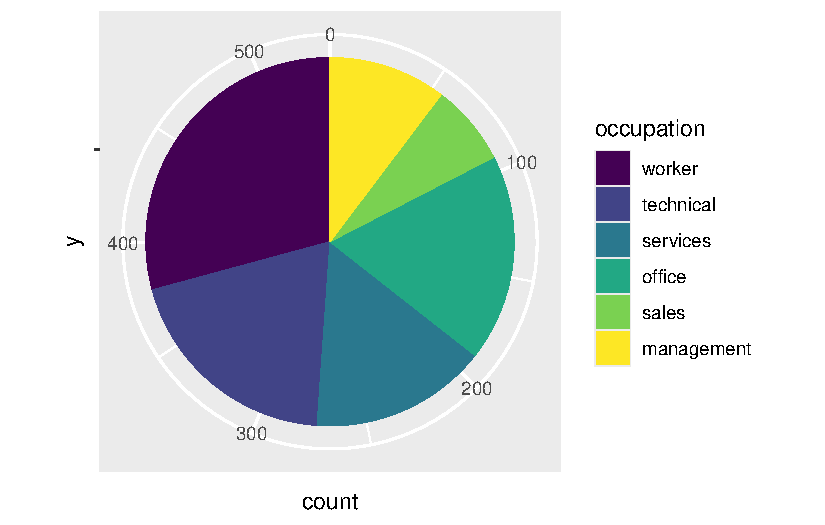
\includegraphics[keepaspectratio]{basicstats_files/figure-pdf/unnamed-chunk-42-1.pdf}}

What is going on with the \texttt{theta\ =\ "x"} argument? In a polar
coordinate system, \(\theta\) (or theta) is the term used to refer to
the angle of a line radiating from the center of the coordinate system.
In the original stacked bar chart, the x-axis was counting how many
people were in each group, so the \texttt{theta\ =\ "x"} argument is
telling \texttt{ggplot()} to use the x variable from the stacked chart
to determine the angles of the wedges. So the ugly thin white line
around your pie chart? That's actually your x-axis!

With pie charts, you often want to use the \texttt{theme\_void()}
argument to get rid of all backgrounds and axes and such, and add the
stuff you want in manually:

\begin{Shaded}
\begin{Highlighting}[]
\NormalTok{CPS1985 }\SpecialCharTok{|\textgreater{}}  
  \FunctionTok{ggplot}\NormalTok{(}\FunctionTok{aes}\NormalTok{(}\AttributeTok{y =} \StringTok{""}\NormalTok{, }\AttributeTok{fill =}\NormalTok{ occupation)) }\SpecialCharTok{+}
  \FunctionTok{geom\_bar}\NormalTok{() }\SpecialCharTok{+}
  \FunctionTok{theme\_void}\NormalTok{() }\SpecialCharTok{+}
  \FunctionTok{scale\_fill\_viridis\_d}\NormalTok{() }\SpecialCharTok{+}
  \FunctionTok{coord\_polar}\NormalTok{(}\AttributeTok{theta =} \StringTok{"x"}\NormalTok{) }\SpecialCharTok{+}
  \FunctionTok{labs}\NormalTok{(}\AttributeTok{title =} \StringTok{"Distribution of Occupation Types"}\NormalTok{,}
       \AttributeTok{subtitle =} \StringTok{"Data from 1985 CPS, n=534"}\NormalTok{,}
       \AttributeTok{fill =} \StringTok{"Occupation"}\NormalTok{)}
\end{Highlighting}
\end{Shaded}

\pandocbounded{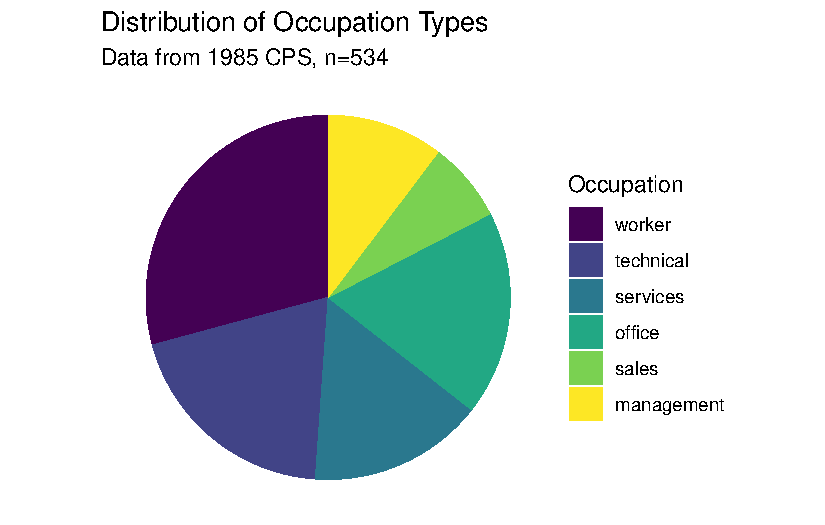
\includegraphics[keepaspectratio]{basicstats_files/figure-pdf/unnamed-chunk-43-1.pdf}}

\subsubsection{Donut Charts}\label{donut-charts}

We can use this methodology to make some donut charts too. A donut chart
is a pie chart with a hole in it. Because somebody thought ``how can we
make a pie chart worse?'' But\ldots you've come this far. Why not see
what embracing evil really looks like?

\begin{center}

\includegraphics[width=0.6\linewidth,height=\textheight,keepaspectratio]{images/donut.jpg}
\end{center}

We start by adjusting our \texttt{aes()} call to have \texttt{y\ =\ 2}.
The key insight is that you're setting up a coordinate system where you
can then ``cut out'' the middle. The specific number matters because it
defines your working space, but the exact value (2, 5, etc.) is flexible
based on what proportions you want to achieve. As a rule of thumb, the
skinnier the donut, the bigger the \texttt{y}.

Now that \texttt{y} is a number, we can use the \texttt{ylim()} argument
to cut out our donut hole. The first number in \texttt{ylim()}
determines how big a hole we cut--it has to be less than \texttt{y} but
bigger than 0, and smaller numbers mean we cut bigger holes. The second
number controls how much empty space you want around your donut;
generally you don't want to go more than 0.5 bigger than your \texttt{y}
value. The code below sets \texttt{ylim(0.2,\ 2.5)}, and the proportions
seem reasonably nice.

\begin{Shaded}
\begin{Highlighting}[]
\NormalTok{CPS1985 }\SpecialCharTok{|\textgreater{}} 
  \FunctionTok{ggplot}\NormalTok{(}\FunctionTok{aes}\NormalTok{(}\AttributeTok{y =} \DecValTok{2}\NormalTok{, }\AttributeTok{fill =}\NormalTok{ occupation)) }\SpecialCharTok{+}
  \FunctionTok{geom\_bar}\NormalTok{() }\SpecialCharTok{+}
  \FunctionTok{theme\_void}\NormalTok{() }\SpecialCharTok{+}
  \FunctionTok{scale\_fill\_viridis\_d}\NormalTok{() }\SpecialCharTok{+}
  \FunctionTok{coord\_polar}\NormalTok{(}\AttributeTok{theta =} \StringTok{"x"}\NormalTok{) }\SpecialCharTok{+}
  \FunctionTok{labs}\NormalTok{(}\AttributeTok{title =} \StringTok{"Distribution of Occupation Types"}\NormalTok{,}
       \AttributeTok{subtitle =} \StringTok{"Data from 1985 CPS, n=534"}\NormalTok{,}
       \AttributeTok{fill =} \StringTok{"Occupation"}\NormalTok{) }\SpecialCharTok{+}
  \FunctionTok{ylim}\NormalTok{(}\FloatTok{0.2}\NormalTok{, }\FloatTok{2.5}\NormalTok{)}
\end{Highlighting}
\end{Shaded}

\pandocbounded{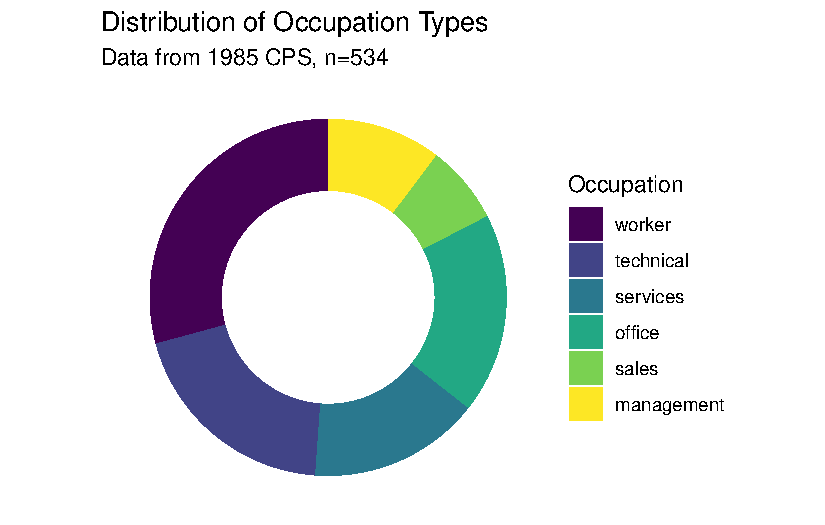
\includegraphics[keepaspectratio]{basicstats_files/figure-pdf/unnamed-chunk-45-1.pdf}}

Feel free to play with the \texttt{y\ =\ 2} option and the
\texttt{ylim()} parameters to see how you can control the size and shape
of the donut. For example, making \texttt{y} (and the corresponding
upper limit in \texttt{ylim()}) bigger makes your donut skinnier:

\begin{Shaded}
\begin{Highlighting}[]
\NormalTok{CPS1985 }\SpecialCharTok{|\textgreater{}} 
  \FunctionTok{ggplot}\NormalTok{(}\FunctionTok{aes}\NormalTok{(}\AttributeTok{y =} \DecValTok{5}\NormalTok{, }\AttributeTok{fill =}\NormalTok{ occupation)) }\SpecialCharTok{+}
  \FunctionTok{geom\_bar}\NormalTok{() }\SpecialCharTok{+}
  \FunctionTok{theme\_void}\NormalTok{() }\SpecialCharTok{+}
  \FunctionTok{scale\_fill\_viridis\_d}\NormalTok{() }\SpecialCharTok{+}
  \FunctionTok{coord\_polar}\NormalTok{(}\AttributeTok{theta =} \StringTok{"x"}\NormalTok{) }\SpecialCharTok{+}
  \FunctionTok{labs}\NormalTok{(}\AttributeTok{title =} \StringTok{"Distribution of Occupation Types"}\NormalTok{,}
       \AttributeTok{subtitle =} \StringTok{"Data from 1985 CPS, n=534"}\NormalTok{,}
       \AttributeTok{fill =} \StringTok{"Occupation"}\NormalTok{) }\SpecialCharTok{+}
  \FunctionTok{ylim}\NormalTok{(.}\DecValTok{2}\NormalTok{, }\FloatTok{5.5}\NormalTok{)}
\end{Highlighting}
\end{Shaded}

\pandocbounded{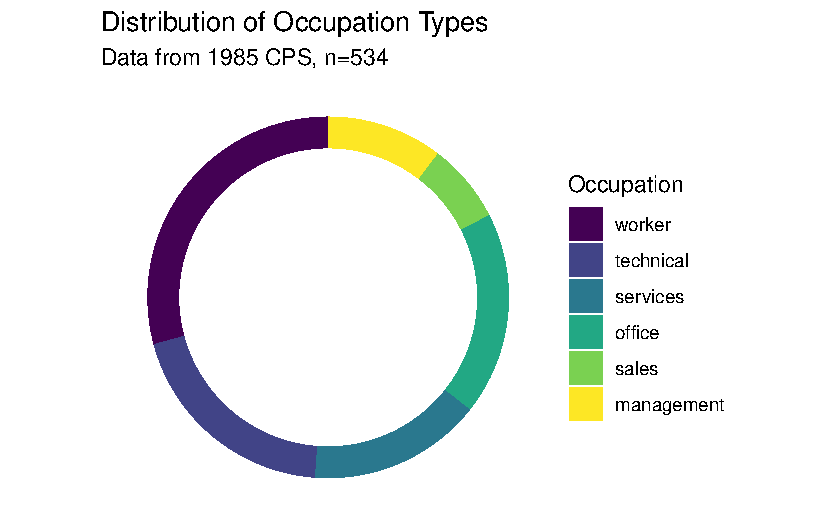
\includegraphics[keepaspectratio]{basicstats_files/figure-pdf/unnamed-chunk-46-1.pdf}}

\subsection{Scatter Plots}\label{scatter-plots}

Scatter plots are useful for looking at the relationship between 2
numerical (preferably continuous) variables. Because there is only 1
continuous variable in the \texttt{CPS1985} dataset (wage, the rest are
discrete), let's switch to using the \texttt{vote1} dataset from the
\texttt{wooldridge} package. To see what is in this, type
\texttt{?vote1} in your console. We might also want to get a quick
overview of the data with the \texttt{head(vote1)} command:

\begin{Shaded}
\begin{Highlighting}[]
\FunctionTok{head}\NormalTok{(vote1)}
\end{Highlighting}
\end{Shaded}

\begin{verbatim}
  state district democA voteA expendA expendB prtystrA lexpendA lexpendB
1    AL        7      1    68 328.296   8.737       41 5.793916 2.167567
2    AK        1      0    62 626.377 402.477       60 6.439952 5.997638
3    AZ        2      1    73  99.607   3.065       55 4.601233 1.120048
4    AZ        3      0    69 319.690  26.281       64 5.767352 3.268846
5    AR        3      0    75 159.221  60.054       66 5.070293 4.095244
6    AR        4      1    69 570.155  21.393       46 6.345908 3.063064
    shareA
1 97.40767
2 60.88104
3 97.01476
4 92.40370
5 72.61247
6 96.38355
\end{verbatim}

This is a pretty fun dataset because it allows us to look at the extent
to which money influences elections in the US.

Let's look at the relationship between the share of campaign
expenditures (\texttt{shareA}) and vote share received (\texttt{voteA}).
We need to set \texttt{x} and \texttt{y} aesthetics, and the geometry of
a scatterplot is \texttt{geom\_point()}:

\begin{Shaded}
\begin{Highlighting}[]
\NormalTok{vote1 }\SpecialCharTok{|\textgreater{}} 
  \FunctionTok{ggplot}\NormalTok{(}\FunctionTok{aes}\NormalTok{(}\AttributeTok{x =}\NormalTok{ shareA, }\AttributeTok{y =}\NormalTok{ voteA)) }\SpecialCharTok{+}
  \FunctionTok{geom\_point}\NormalTok{()}
\end{Highlighting}
\end{Shaded}

\pandocbounded{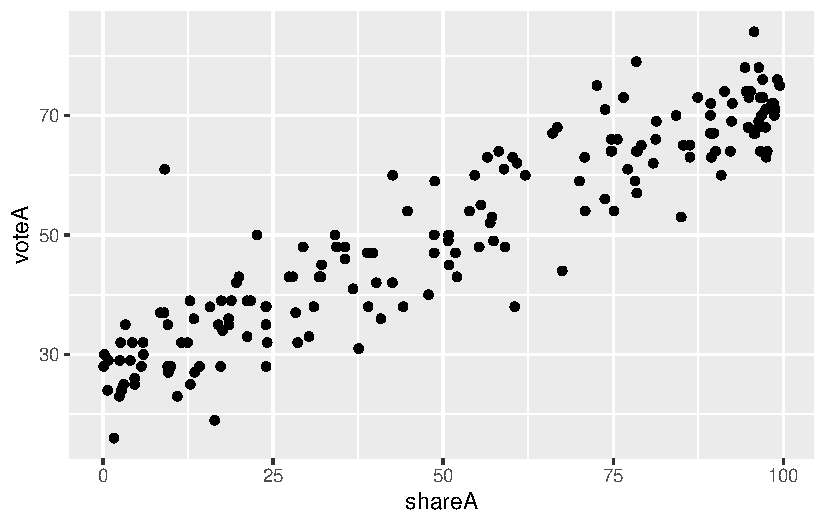
\includegraphics[keepaspectratio]{basicstats_files/figure-pdf/unnamed-chunk-52-1.pdf}}

Why \texttt{(x\ =\ shareA,\ y\ =\ voteA)} and not
\texttt{(y\ =\ shareA,\ x\ =\ voteA)}? In this case, theory tells that
vote share should be the \textbf{dependent variable} and campaign
expenditures should be the \textbf{independent variable}, and when
graphing the generally accepted norm is to put the DV (dependent
variable) on the Y axis.

\begin{tcolorbox}[enhanced jigsaw, colframe=quarto-callout-tip-color-frame, breakable, arc=.35mm, bottomtitle=1mm, bottomrule=.15mm, colbacktitle=quarto-callout-tip-color!10!white, rightrule=.15mm, colback=white, opacityback=0, opacitybacktitle=0.6, coltitle=black, left=2mm, toptitle=1mm, toprule=.15mm, titlerule=0mm, leftrule=.75mm, title=\textcolor{quarto-callout-tip-color}{\faLightbulb}\hspace{0.5em}{Data Storytelling: R Doesn't Know Causality}]

Here's the thing: R doesn't get causality. You could totally flip this
and put \texttt{voteA} on the x-axis and \texttt{shareA} on the y-axis,
and R would happily create a perfectly functional scatterplot.

But you know something about how the world works. This is what separates
``I can make graphs in R'' from ``I can actually analyze data.'' Sure,
anyone can plot variables against each other, but understanding which
variable is trying to influence which requires you to think about the
real world beyond your computer screen. Does campaign spending influence
election outcomes, or do election outcomes magically determine how much
money campaigns spent months earlier?

Spoiler alert: time generally moves forward, not backward. R doesn't
know this. Maybe R thinks that election results magically travel
backward through time to force donors in the past to give money to the
winners. It's like a
\href{https://intothespiderverse.fandom.com/wiki/Canon_Events}{Spider-verse
Canon Event} for all R knows. R quite literally just sees numbers and
does math. It just follows orders.

Whether you're looking at marketing spend vs.~sales, study time vs.~test
scores, or coffee consumption vs.~productivity (definitely a causal
relationship there), your job is to bring some actual knowledge about
how things work to the table. R will crunch the numbers, but it won't
tell you what makes sense.

\end{tcolorbox}

Perhaps you want to see the line of best fit? We can add the
\texttt{geom\_smooth(method\ =\ lm)} layer to our \texttt{ggplot()}:

\begin{Shaded}
\begin{Highlighting}[]
\NormalTok{vote1 }\SpecialCharTok{|\textgreater{}} 
  \FunctionTok{ggplot}\NormalTok{(}\FunctionTok{aes}\NormalTok{(}\AttributeTok{x =}\NormalTok{ shareA, }\AttributeTok{y =}\NormalTok{ voteA)) }\SpecialCharTok{+}
  \FunctionTok{geom\_point}\NormalTok{() }\SpecialCharTok{+}
  \FunctionTok{geom\_smooth}\NormalTok{(}\AttributeTok{method =}\NormalTok{ lm)}
\end{Highlighting}
\end{Shaded}

\begin{verbatim}
`geom_smooth()` using formula = 'y ~ x'
\end{verbatim}

\pandocbounded{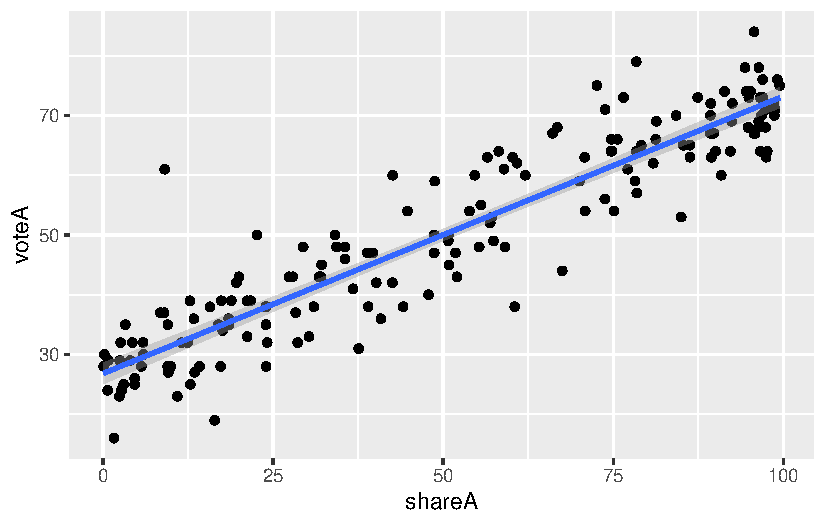
\includegraphics[keepaspectratio]{basicstats_files/figure-pdf/unnamed-chunk-53-1.pdf}}

\begin{tcolorbox}[enhanced jigsaw, colframe=quarto-callout-tip-color-frame, breakable, arc=.35mm, bottomtitle=1mm, bottomrule=.15mm, colbacktitle=quarto-callout-tip-color!10!white, rightrule=.15mm, colback=white, opacityback=0, opacitybacktitle=0.6, coltitle=black, left=2mm, toptitle=1mm, toprule=.15mm, titlerule=0mm, leftrule=.75mm, title=\textcolor{quarto-callout-tip-color}{\faLightbulb}\hspace{0.5em}{May the Format be With You: Silencing Chatty Functions}]

When you run \texttt{geom\_smooth()}, R likes to tell you it's
\texttt{using\ formula\ =\ y\ \textasciitilde{}\ x}\ldots basically just
confirming it's drawing a straight line. While this transparency is
nice, it clutters your output. If you are incorporating lines of best
fit into charts in a Quarto document, you almost always want to add
\texttt{\#\textbar{}\ message:\ false} to your code chunk to tell R to
zip it.

For the scatter diagram above, I didn't suppress the message, but I will
do so for the rest of them.

\end{tcolorbox}

As before, we can add elements if we want here. For example, maybe we
want to highlight which party each candidate belongs to. The
\texttt{democA} variable uses 1 for Democrats and 0 for Republicans, but
\texttt{ggplot()} wants factors for color coding, so we need to wrap it
in \texttt{as.factor()}:

\begin{Shaded}
\begin{Highlighting}[]
\NormalTok{vote1 }\SpecialCharTok{|\textgreater{}} 
  \FunctionTok{ggplot}\NormalTok{(}\FunctionTok{aes}\NormalTok{(}\AttributeTok{x =}\NormalTok{ shareA, }\AttributeTok{y =}\NormalTok{ voteA, }\AttributeTok{color =} \FunctionTok{as.factor}\NormalTok{(democA))) }\SpecialCharTok{+}
  \FunctionTok{geom\_point}\NormalTok{() }\SpecialCharTok{+}
  \FunctionTok{labs}\NormalTok{(}\AttributeTok{title =} \StringTok{"Campaign Spending vs Vote Share by Party"}\NormalTok{,}
       \AttributeTok{x =} \StringTok{"Share of Campaign Expenditures"}\NormalTok{, }
       \AttributeTok{y =} \StringTok{"Vote Share"}\NormalTok{,}
       \AttributeTok{color =} \StringTok{"Party"}\NormalTok{)}
\end{Highlighting}
\end{Shaded}

\pandocbounded{\includegraphics[keepaspectratio]{basicstats_files/figure-pdf/unnamed-chunk-54-1.pdf}}

Let's make this more readable by using proper party colors and labels:

\begin{Shaded}
\begin{Highlighting}[]
\NormalTok{vote1 }\SpecialCharTok{|\textgreater{}} 
  \FunctionTok{ggplot}\NormalTok{(}\FunctionTok{aes}\NormalTok{(}\AttributeTok{x =}\NormalTok{ shareA, }\AttributeTok{y =}\NormalTok{ voteA, }\AttributeTok{color =} \FunctionTok{as.factor}\NormalTok{(democA))) }\SpecialCharTok{+}
  \FunctionTok{geom\_point}\NormalTok{() }\SpecialCharTok{+}
  \FunctionTok{scale\_color\_manual}\NormalTok{(}\AttributeTok{values =} \FunctionTok{c}\NormalTok{(}\StringTok{"0"} \OtherTok{=} \StringTok{"\#db2b27"}\NormalTok{, }\StringTok{"1"} \OtherTok{=} \StringTok{"\#1696d2"}\NormalTok{),}
                     \AttributeTok{labels =} \FunctionTok{c}\NormalTok{(}\StringTok{"0"} \OtherTok{=} \StringTok{"Republican"}\NormalTok{, }\StringTok{"1"} \OtherTok{=} \StringTok{"Democrat"}\NormalTok{)) }\SpecialCharTok{+}
  \FunctionTok{labs}\NormalTok{(}\AttributeTok{title =} \StringTok{"Campaign Spending vs Vote Share by Party"}\NormalTok{,}
       \AttributeTok{x =} \StringTok{"Share of Campaign Expenditures"}\NormalTok{, }
       \AttributeTok{y =} \StringTok{"Vote Share"}\NormalTok{,}
       \AttributeTok{color =} \StringTok{"Party"}\NormalTok{) }\SpecialCharTok{+}
  \FunctionTok{theme\_minimal}\NormalTok{()}
\end{Highlighting}
\end{Shaded}

\pandocbounded{\includegraphics[keepaspectratio]{basicstats_files/figure-pdf/unnamed-chunk-55-1.pdf}}

\begin{tcolorbox}[enhanced jigsaw, colframe=quarto-callout-tip-color-frame, breakable, arc=.35mm, bottomtitle=1mm, bottomrule=.15mm, colbacktitle=quarto-callout-tip-color!10!white, rightrule=.15mm, colback=white, opacityback=0, opacitybacktitle=0.6, coltitle=black, left=2mm, toptitle=1mm, toprule=.15mm, titlerule=0mm, leftrule=.75mm, title=\textcolor{quarto-callout-tip-color}{\faLightbulb}\hspace{0.5em}{May the Format Be With You: Brand Consistency (or: How to Look Like You
Actually Know What You're Doing)}]

Want to avoid looking like an amateur who just discovered hex codes?
Here's a pro tip from the design world: stop typing the same color codes
over and over like some kind of data visualization peasant.

Notice how I just typed \texttt{"\#db2b27"} and \texttt{"\#1696d2"} in
the graph above? Sure, I could keep doing that throughout the entire
document, making typos, forgetting exact codes, and writing code that
will produce a result that looks sloppy or lazy. Or I could do what the
pros do and set up my colors as variables at the beginning:

\begin{Shaded}
\begin{Highlighting}[]
\CommentTok{\# Political party colors {-} define once, use everywhere}
\NormalTok{dem\_blue }\OtherTok{\textless{}{-}} \StringTok{"\#1696d2"}
\NormalTok{rep\_red }\OtherTok{\textless{}{-}} \StringTok{"\#db2b27"}
\end{Highlighting}
\end{Shaded}

Which is honestly just being lazy in a smart way. Because then,
throughout your document, you can simply reference these variables. For
example:

\begin{Shaded}
\begin{Highlighting}[]
\FunctionTok{ggplot}\NormalTok{(data, }\FunctionTok{aes}\NormalTok{(}\AttributeTok{x =}\NormalTok{ category, }\AttributeTok{y =}\NormalTok{ value)) }\SpecialCharTok{+}
  \FunctionTok{geom\_bar}\NormalTok{(}\AttributeTok{fill =}\NormalTok{ dem\_blue, }\AttributeTok{color =}\NormalTok{ rep\_red) }\SpecialCharTok{+}
  \FunctionTok{theme\_minimal}\NormalTok{()}
\end{Highlighting}
\end{Shaded}

Why is this approach so much better?

\begin{itemize}
\tightlist
\item
  Consistency: All your graphs will use exactly the same colors - no
  more ``is this the right shade of blue?'' moments
\item
  Efficiency: No more hunting for hex codes or copying/pasting from old
  graphs
\item
  Flexibility: Need to rebrand everything? In my lecture slides for my
  Principles of Macro classes, I set up my documents with variables
  named color1 through color5; all I need to do is change the colors in
  those five lines at the top, and every color in the document gets an
  instant makeover.
\item
  Professional vibes: Your document gets that polished, branded look
  that screams ``I know what I'm doing''
\end{itemize}

Whether you're trying to impress a boss, avoid getting roasted by your
professor, or just want to make something look super professional, this
simple technique will level up your work significantly.

\end{tcolorbox}

Let's put this advice into action. First, we'll set up our color
variables:

\begin{Shaded}
\begin{Highlighting}[]
\CommentTok{\# Political party colors {-} define once, use everywhere}
\NormalTok{dem\_blue }\OtherTok{\textless{}{-}} \StringTok{"\#1696d2"}
\NormalTok{rep\_red }\OtherTok{\textless{}{-}} \StringTok{"\#db2b27"}
\end{Highlighting}
\end{Shaded}

Now we can create separate graphs for the Democrats and Republicans
using facet\_wrap() with our color variables:

\begin{Shaded}
\begin{Highlighting}[]
\NormalTok{vote1 }\SpecialCharTok{|\textgreater{}} 
  \FunctionTok{ggplot}\NormalTok{(}\FunctionTok{aes}\NormalTok{(}\AttributeTok{x =}\NormalTok{ shareA, }\AttributeTok{y =}\NormalTok{ voteA)) }\SpecialCharTok{+}
  \FunctionTok{geom\_point}\NormalTok{(}\FunctionTok{aes}\NormalTok{(}\AttributeTok{color =} \FunctionTok{as.factor}\NormalTok{(democA))) }\SpecialCharTok{+}
  \FunctionTok{scale\_color\_manual}\NormalTok{(}\AttributeTok{values =} \FunctionTok{c}\NormalTok{(}\StringTok{"0"} \OtherTok{=}\NormalTok{ rep\_red, }\StringTok{"1"} \OtherTok{=}\NormalTok{ dem\_blue)) }\SpecialCharTok{+}
  \FunctionTok{facet\_wrap}\NormalTok{(}\SpecialCharTok{\textasciitilde{}}\NormalTok{democA, }
             \AttributeTok{labeller =} \FunctionTok{labeller}\NormalTok{(}\AttributeTok{democA =} \FunctionTok{c}\NormalTok{(}\StringTok{"0"} \OtherTok{=} \StringTok{"Republicans"}\NormalTok{, }\StringTok{"1"} \OtherTok{=} \StringTok{"Democrats"}\NormalTok{))) }\SpecialCharTok{+}
  \FunctionTok{labs}\NormalTok{(}\AttributeTok{title =} \StringTok{"Campaign Spending vs Vote Share"}\NormalTok{,}
       \AttributeTok{x =} \StringTok{"Share of Campaign Expenditures"}\NormalTok{, }
       \AttributeTok{y =} \StringTok{"Vote Share"}\NormalTok{) }\SpecialCharTok{+}
  \FunctionTok{theme\_minimal}\NormalTok{() }\SpecialCharTok{+}
  \FunctionTok{theme}\NormalTok{(}\AttributeTok{legend.position =} \StringTok{"none"}\NormalTok{)  }\CommentTok{\# Remove legend since facet labels tell the story}
\end{Highlighting}
\end{Shaded}

\pandocbounded{\includegraphics[keepaspectratio]{basicstats_files/figure-pdf/unnamed-chunk-59-1.pdf}}

All in all, R has some extremely powerful graphing capabilities that go
well beyond what something like Excel is capable of. These days, when
people ask me for help making graphs in Excel, I cringe a little because
I know how much better it would look in R. Once you wrap your head
around the \hyperref[grammar-of-graphics]{Grammar of Graphics} \ldots{}
aesthetics, layers, themes, etc. \ldots{} \texttt{ggplot()} becomes way
more intuitive than clicking through Excel's endless and
counterintuitive menu system. Sure, there's a learning curve up front,
but the payoff is graphs that actually look professional and really,
really, ridiculously good looking.

\section{Summarizing Data
Numerically}\label{summarizing-data-numerically}

Now that we have seen an overview of the graphical capabilities, let's
turn to numerical summaries. We return to the \texttt{CPS1985} dataset
so we can look at both numerical and categorical variables.

\subsection{Categorical Variables}\label{categorical-variables}

Let's start with categorical variables and focus on occupation.
Categorical variables are summarized with frequencies or proportions.
The \texttt{table()} command (we saw this above when we made
\hyperref[bar-and-pie-charts]{Bar and Pie Charts}) works to create
these; by default, \texttt{table()} summarizes counts.

\begin{Shaded}
\begin{Highlighting}[]
\FunctionTok{table}\NormalTok{(CPS1985}\SpecialCharTok{$}\NormalTok{occupation)}
\end{Highlighting}
\end{Shaded}

\begin{verbatim}

    worker  technical   services     office      sales management 
       156        105         83         97         38         55 
\end{verbatim}

Here's the same analysis of the sector variable:

\begin{Shaded}
\begin{Highlighting}[]
\FunctionTok{table}\NormalTok{(CPS1985}\SpecialCharTok{$}\NormalTok{sector)}
\end{Highlighting}
\end{Shaded}

\begin{verbatim}

manufacturing  construction         other 
           99            24           411 
\end{verbatim}

OK, typing CPS1985\$ over and over is getting pretty cumbersome. There's
a shortcut for this called \texttt{attach()} that can make your life
easier when working with a single dataset.

\begin{tcolorbox}[enhanced jigsaw, colframe=quarto-callout-tip-color-frame, breakable, arc=.35mm, bottomtitle=1mm, bottomrule=.15mm, colbacktitle=quarto-callout-tip-color!10!white, rightrule=.15mm, colback=white, opacityback=0, opacitybacktitle=0.6, coltitle=black, left=2mm, toptitle=1mm, toprule=.15mm, titlerule=0mm, leftrule=.75mm, title=\textcolor{quarto-callout-tip-color}{\faLightbulb}\hspace{0.5em}{Tip from the Helpdesk: To Attach or Not to Attach?}]

The attach() function lets you refer to variables in a dataset without
typing the dataset name every time. So instead of CPS1985\$occupation,
you could just type occupation. Sounds great, right?

So, let's start with why this doesn't work (yet):

\begin{Shaded}
\begin{Highlighting}[]
\FunctionTok{table}\NormalTok{(occupation)}
\end{Highlighting}
\end{Shaded}

\begin{verbatim}
Error in eval(expr, envir, enclos): object 'occupation' not found
\end{verbatim}

Why not? Because R is looking for a variable called \texttt{occupation}
to make a \texttt{table()} with, and it doesn't know where it is. R
isn't smart enough to look inside of the \texttt{CPS1985} dataset for a
variable called \texttt{occupation}, so it spits out an error. When I
\texttt{attach()} the \texttt{CPS1985} dataset, I'm simply telling R
that it should feel free to look inside the \texttt{CPS1985} dataset for
variables. In a lot of ways, it's kinda like how libraries work. When I
turn on R, it doesn't know what the heck a \texttt{ggplot()} is. When I
run \texttt{library(tidyverse)}, I'm telling R to look inside the
\texttt{tidyverse} family of functions when I give it a command. If I
run \texttt{ggplot()} \emph{after} I load the \texttt{tidyverse}, R will
be able to figure out what \texttt{ggplot()} means.

So, let's attach the dataset and see what happens with that same funcion
that broke earlier.

\begin{Shaded}
\begin{Highlighting}[]
\FunctionTok{attach}\NormalTok{(CPS1985)}
\FunctionTok{table}\NormalTok{(occupation)  }\CommentTok{\# No more CPS1985$ needed!}
\end{Highlighting}
\end{Shaded}

\begin{verbatim}
occupation
    worker  technical   services     office      sales management 
       156        105         83         97         38         55 
\end{verbatim}

Ha! Now, you might be wondering why I didn't start with this? Way to
bury the lede, right?

While attach() can be a useful crutch when you're learning R and is fine
when you're only working with a single dataset, it can create confusion
in larger projects. What happens when you have multiple datasets with
variables that have the same name? Which age variable is R using - the
one from dataset A or dataset B?

Honestly, it's probably worth just biting the bullet and learning to use
the \texttt{\$} notation. You'll see both approaches in the wild, but
explicit \texttt{dataset\$variable} notation will save you headaches
down the road when your projects get more complex. Your future self will
thank you for the clarity!

For this book, I plan on sticking with the explicit notation, but I
reserve the right to switch if the typing gets really tedious or I just
get really lazy.

\end{tcolorbox}

Let's convert those counts to proportions. The easiest way is to divide
your totals by the size of the dataset:

\begin{Shaded}
\begin{Highlighting}[]
\FunctionTok{table}\NormalTok{(CPS1985}\SpecialCharTok{$}\NormalTok{occupation) }\SpecialCharTok{/} \FunctionTok{nrow}\NormalTok{(CPS1985)}
\end{Highlighting}
\end{Shaded}

\begin{verbatim}

    worker  technical   services     office      sales management 
0.29213483 0.19662921 0.15543071 0.18164794 0.07116105 0.10299625 
\end{verbatim}

You can also produce contingency (two-way) tables that look at the
intersection of two categorical variables:

\begin{Shaded}
\begin{Highlighting}[]
\FunctionTok{table}\NormalTok{(CPS1985}\SpecialCharTok{$}\NormalTok{occupation, CPS1985}\SpecialCharTok{$}\NormalTok{gender)}
\end{Highlighting}
\end{Shaded}

\begin{verbatim}
            
             male female
  worker      126     30
  technical    53     52
  services     34     49
  office       21     76
  sales        21     17
  management   34     21
\end{verbatim}

This shows us the breakdown of gender within each occupation category in
1985. Now we can see, for example, that the sales and technical roles
were roughly evenly split between the genders, while workers tended to
be male and office jobs went to females.

\subsection{Numerical Variables}\label{numerical-variables}

While we are limited in how we describe categorical variables, we have
lots of options with respect to numerical variables. Let's analyze the
wage variable.

Arithmetic means are calculated with the \texttt{mean()} function.

\begin{Shaded}
\begin{Highlighting}[]
\FunctionTok{mean}\NormalTok{(CPS1985}\SpecialCharTok{$}\NormalTok{wage)}
\end{Highlighting}
\end{Shaded}

\begin{verbatim}
[1] 9.024064
\end{verbatim}

A trimmed mean drops the outliers from the top and bottom of the data.
For example, if we type:

\begin{Shaded}
\begin{Highlighting}[]
\FunctionTok{mean}\NormalTok{(CPS1985}\SpecialCharTok{$}\NormalTok{wage, }\AttributeTok{trim =} \FloatTok{0.05}\NormalTok{)}
\end{Highlighting}
\end{Shaded}

\begin{verbatim}
[1] 8.544212
\end{verbatim}

We tell R to drop the 5\% of the lowest wages and 5\% of the highest
wages from the data and calculate the mean of the middle 90\%. Sometimes
this makes sense when you are looking at a data set with a lot of skew.
Another thing we might do to get a measure of central tendency for
skewed data is to calculate a \texttt{median()}.

\begin{Shaded}
\begin{Highlighting}[]
\FunctionTok{median}\NormalTok{(CPS1985}\SpecialCharTok{$}\NormalTok{wage)}
\end{Highlighting}
\end{Shaded}

\begin{verbatim}
[1] 7.78
\end{verbatim}

Generally speaking, medians are the preferred measure of central
tendency in cases with skewed data because medians are far less
sensitive to the presence of outliers in the data\ldots{}

\begin{center}
\includegraphics[width=0.75\linewidth,height=\textheight,keepaspectratio]{images/meanoutlier.jpg}
\end{center}

Variance and Standard Deviation are calculated with \texttt{var()} and
\texttt{sd()}, respectively.

\begin{Shaded}
\begin{Highlighting}[]
\FunctionTok{var}\NormalTok{(CPS1985}\SpecialCharTok{$}\NormalTok{wage)}
\end{Highlighting}
\end{Shaded}

\begin{verbatim}
[1] 26.41032
\end{verbatim}

\begin{Shaded}
\begin{Highlighting}[]
\FunctionTok{sd}\NormalTok{(CPS1985}\SpecialCharTok{$}\NormalTok{wage)}
\end{Highlighting}
\end{Shaded}

\begin{verbatim}
[1] 5.139097
\end{verbatim}

Don't forget, the standard deviation is the square root of the variance!

\begin{Shaded}
\begin{Highlighting}[]
\FunctionTok{sd}\NormalTok{(CPS1985}\SpecialCharTok{$}\NormalTok{wage)}\SpecialCharTok{\^{}}\DecValTok{2}
\end{Highlighting}
\end{Shaded}

\begin{verbatim}
[1] 26.41032
\end{verbatim}

\begin{Shaded}
\begin{Highlighting}[]
\FunctionTok{sqrt}\NormalTok{(}\FunctionTok{var}\NormalTok{(CPS1985}\SpecialCharTok{$}\NormalTok{wage))}
\end{Highlighting}
\end{Shaded}

\begin{verbatim}
[1] 5.139097
\end{verbatim}

Minima and maxima can be calculated with the \texttt{min()} and
\texttt{max()} commands.

\begin{Shaded}
\begin{Highlighting}[]
\FunctionTok{min}\NormalTok{(CPS1985}\SpecialCharTok{$}\NormalTok{wage)}
\end{Highlighting}
\end{Shaded}

\begin{verbatim}
[1] 1
\end{verbatim}

\begin{Shaded}
\begin{Highlighting}[]
\FunctionTok{max}\NormalTok{(CPS1985}\SpecialCharTok{$}\NormalTok{wage)}
\end{Highlighting}
\end{Shaded}

\begin{verbatim}
[1] 44.5
\end{verbatim}

You can get both easily if you want using \texttt{range()}

\begin{Shaded}
\begin{Highlighting}[]
\FunctionTok{range}\NormalTok{(CPS1985}\SpecialCharTok{$}\NormalTok{wage)}
\end{Highlighting}
\end{Shaded}

\begin{verbatim}
[1]  1.0 44.5
\end{verbatim}

Measures of position (quartiles, percentiles, etc) can be obtained
through the \texttt{quantile()} function. You need to pass through a
\texttt{probs} argument to tell it which quantile you want.

If you just want one specific quantile--in this case the first
quartile--you type:

\begin{Shaded}
\begin{Highlighting}[]
\FunctionTok{quantile}\NormalTok{(CPS1985}\SpecialCharTok{$}\NormalTok{wage, .}\DecValTok{25}\NormalTok{)}
\end{Highlighting}
\end{Shaded}

\begin{verbatim}
 25% 
5.25 
\end{verbatim}

You can also use the \texttt{c()} language we've seen before to get
multiple quantiles at once. For example, if we want the 10th, 25th,
50th, 75th, and 90th percentile, we type:

\begin{Shaded}
\begin{Highlighting}[]
\FunctionTok{quantile}\NormalTok{(CPS1985}\SpecialCharTok{$}\NormalTok{wage, }\AttributeTok{probs =} \FunctionTok{c}\NormalTok{(.}\DecValTok{1}\NormalTok{, .}\DecValTok{25}\NormalTok{, .}\DecValTok{5}\NormalTok{, .}\DecValTok{75}\NormalTok{, .}\DecValTok{9}\NormalTok{))}
\end{Highlighting}
\end{Shaded}

\begin{verbatim}
   10%    25%    50%    75%    90% 
 4.000  5.250  7.780 11.250 15.275 
\end{verbatim}

The minimum and maximum of the data can also be obtained using the 0th
and 100th quartile:

\begin{Shaded}
\begin{Highlighting}[]
\FunctionTok{quantile}\NormalTok{(CPS1985}\SpecialCharTok{$}\NormalTok{wage, }\AttributeTok{probs =} \FunctionTok{c}\NormalTok{(}\DecValTok{0}\NormalTok{,}\DecValTok{1}\NormalTok{))}
\end{Highlighting}
\end{Shaded}

\begin{verbatim}
  0% 100% 
 1.0 44.5 
\end{verbatim}

Correlation coefficients can be calculated using \texttt{cor()}. Here is
the correlation between education and wage:

\begin{Shaded}
\begin{Highlighting}[]
\FunctionTok{cor}\NormalTok{(CPS1985}\SpecialCharTok{$}\NormalTok{wage, CPS1985}\SpecialCharTok{$}\NormalTok{education)}
\end{Highlighting}
\end{Shaded}

\begin{verbatim}
[1] 0.3819221
\end{verbatim}

This indicates a moderate positive correlation between the two
variables. We can see this correlation in this graph:

\begin{Shaded}
\begin{Highlighting}[]
\NormalTok{CPS1985 }\SpecialCharTok{|\textgreater{}} \FunctionTok{ggplot}\NormalTok{(}\FunctionTok{aes}\NormalTok{(}\AttributeTok{x =}\NormalTok{ education, }\AttributeTok{y =}\NormalTok{ wage)) }\SpecialCharTok{+}
    \FunctionTok{geom\_point}\NormalTok{() }\SpecialCharTok{+}
    \FunctionTok{geom\_smooth}\NormalTok{(}\AttributeTok{method =}\NormalTok{ lm)}
\end{Highlighting}
\end{Shaded}

\pandocbounded{\includegraphics[keepaspectratio]{basicstats_files/figure-pdf/unnamed-chunk-78-1.pdf}}

By default, R calculates the Pearson correlation, which is appropriate
for interval data. Sometimes you have ordinal data where a Spearman
correlation makes more sense, for example, when the data is a ranking
but not a measure. In this case, the Pearson is quantifying the linear
relationship between education and wage, but a Spearman test simply asks
whether or not higher levels of education are linked to higher wages.

\begin{Shaded}
\begin{Highlighting}[]
\FunctionTok{cor}\NormalTok{(CPS1985}\SpecialCharTok{$}\NormalTok{wage, CPS1985}\SpecialCharTok{$}\NormalTok{education, }\AttributeTok{method =} \StringTok{"spearman"}\NormalTok{)}
\end{Highlighting}
\end{Shaded}

\begin{verbatim}
[1] 0.3813425
\end{verbatim}

In most economic applications, Pearson is more useful.

Don't forget, the summary() command can be useful here too:

\begin{Shaded}
\begin{Highlighting}[]
\FunctionTok{summary}\NormalTok{(CPS1985}\SpecialCharTok{$}\NormalTok{wage)}
\end{Highlighting}
\end{Shaded}

\begin{verbatim}
   Min. 1st Qu.  Median    Mean 3rd Qu.    Max. 
  1.000   5.250   7.780   9.024  11.250  44.500 
\end{verbatim}

The \texttt{stargazer()} package/function makes nicely formatted tables
of summary statistics, but you have to put in a whole dataframe:

\begin{Shaded}
\begin{Highlighting}[]
\FunctionTok{stargazer}\NormalTok{(CPS1985, }\AttributeTok{type =} \StringTok{"text"}\NormalTok{)}
\end{Highlighting}
\end{Shaded}

\begin{verbatim}

===========================================
Statistic   N   Mean  St. Dev.  Min   Max  
-------------------------------------------
wage       534 9.024   5.139   1.000 44.500
education  534 13.019  2.615     2     18  
experience 534 17.822  12.380    0     55  
age        534 36.833  11.727   18     64  
-------------------------------------------
\end{verbatim}

It is also capable of making more visually attractive, publication ready
tables:

\begin{Shaded}
\begin{Highlighting}[]
\FunctionTok{stargazer}\NormalTok{(CPS1985, }\AttributeTok{type =} \StringTok{"html"}\NormalTok{)}
\end{Highlighting}
\end{Shaded}

Statistic

N

Mean

St.~Dev.

Min

Max

wage

534

9.024

5.139

1.000

44.500

education

534

13.019

2.615

2

18

experience

534

17.822

12.380

0

55

age

534

36.833

11.727

18

64

You can't see it in my code chunk, but to get the
\texttt{type\ =\ "html"} to work right the code chunk needs to have an
option of \texttt{\#\textbar{}\ results:\ asis} or else you will get
something funky! We will make extensive use of \texttt{stargazer()}
later in this book, so file away this tip in your brain for later!

\section{Wrapping Up}\label{wrapping-up-2}

This chapter notebook reviewed what is essentially the first half of an
intro to statistics class and introduced how to use R for these
calculations. The next step is to tackle inferential statistics using R,
which we turn to in Chapter~\ref{sec-inferstats}.

\section{End of Chapter Exercises}\label{end-of-chapter-exercises-1}

Charts and Graphs: Ensure that your charts include axis labels and
titles. Use \texttt{ggplot()} for all graphics!!

Throughout this book, datasets are given in the form of
\texttt{package:dataset}. To access them, you first load the relevant
package, and then load the dataset you wish to use. For example, to use
the \texttt{wooldridge:wine} dataset from question 7, you would use the
following commands:

\begin{Shaded}
\begin{Highlighting}[]
\FunctionTok{library}\NormalTok{(wooldridge)}
\FunctionTok{data}\NormalTok{(wine)}
\end{Highlighting}
\end{Shaded}

Bar Charts:

\begin{enumerate}
\def\labelenumi{\arabic{enumi}.}
\item
  Look at \texttt{fivethirtyeight:hiphop\_cand\_lyrics} and make bar
  charts of \texttt{sentiment} for both Donald Trump and Hillary
  Clinton. What does this tell you about how hip-hop artists viewed
  these candidates? What happens if you focus on specific years or break
  down by different sentiment themes?
\item
  Use the \texttt{AER:BankWages} data to make bar charts of
  \texttt{job}. Which job type is the most common in the dataset? Create
  side-by-side or stacked bar charts to examine whether there are
  different patterns between genders. What does this suggest about
  gender representation across different banking positions?
\item
  For the \texttt{AER:BankWages} data, calculate summary statistics for
  \texttt{education} by job type, ethnicity, and gender. Create a
  summary table showing the mean and median years of education for each
  combination. Do the numerical summaries reveal patterns about
  educational requirements or ethnicity/gender differences that weren't
  obvious in your bar charts from question 2? Do different
  genders/ethnicities require more/less education to get the premium
  managerial jobs?
\item
  Create bar charts looking at the distribution of student
  \texttt{gender} and \texttt{ethnicity} in the \texttt{AER:STAR} data.
  Consider making both separate charts and grouped/stacked charts. What
  does this tell you about the student population in this study?
\end{enumerate}

Box Plots and Histograms:

\begin{enumerate}
\def\labelenumi{\arabic{enumi}.}
\setcounter{enumi}{4}
\item
  Using the \texttt{AER:NMES1988} dataset, create a histogram of the
  number of physician office visits (\texttt{visits}) and a box plot
  examining the number of \texttt{visits} by \texttt{health} status.
  What does the distribution of visits look like? How do healthcare
  utilization patterns differ by health status? Are there outliers, and
  what might they represent?
\item
  Using the \texttt{dplyr:starwars} dataset, create a histogram of the
  \texttt{height} of Star Wars characters and a box plot looking at
  \texttt{height} by the \texttt{gender} of the characters. What does
  this tell you about the diversity of character sizes in the Star Wars
  universe? Are there notable differences between genders?
\item
  Using the \texttt{dplyr:starwars} dataset, calculate summary
  statistics (mean, median, standard deviation, quartiles) for
  \texttt{height} by \texttt{gender}. How do these numerical summaries
  compare to what you observed in the box plots from question 5? Which
  measure of central tendency (mean vs.~median) is more appropriate for
  this data and why?
\end{enumerate}

Scatter Plots:

\begin{enumerate}
\def\labelenumi{\arabic{enumi}.}
\setcounter{enumi}{7}
\item
  Use \texttt{datasets:USArrests} to look at the relationship between
  urbanization (\texttt{UrbanPop}) and each of the three measures of
  crime (\texttt{Murder}, \texttt{Assault}, and \texttt{Rape}). Create
  three separate scatter plots. What patterns do you observe? Does
  urbanization appear to be related to crime rates? Which crimes show
  the strongest relationship with urbanization? Including lines of best
  fit might help with this analysis.
\item
  Using \texttt{datasets:USArrests}, calculate correlation coefficients
  between \texttt{UrbanPop} and each crime variable. How do these
  correlations compare to your visual impressions from the scatter plots
  in question 8? Calculate summary statistics (mean, median, standard
  deviation) for each crime type - which crimes show the most
  variability across states?
\item
  Look at the relationship between alcohol consumption
  (\texttt{alcohol}) and \texttt{deaths}, \texttt{heart}, and
  \texttt{liver} in \texttt{wooldridge:wine}. Create three scatter plots
  and consider adding trend lines. What do these relationships suggest
  about the health effects of alcohol consumption? Do the results
  surprise you?
\item
  Using \texttt{wooldridge:meap01}, look at the relationship between
  expenditures per student (\texttt{expp}) and the various test scores
  (\texttt{math4} and \texttt{read4}). Create scatter plots for both
  relationships. Does more spending appear to be associated with better
  test scores? Are there outliers that might represent particularly
  efficient or inefficient school districts?
\end{enumerate}

Thinking about Graphs:

\begin{enumerate}
\def\labelenumi{\arabic{enumi}.}
\setcounter{enumi}{11}
\tightlist
\item
  Short answer: Compare the histogram and boxplots of \texttt{wages}
  above. Which visualization better represents the distribution of
  wages, and why? Consider what each type of graph emphasizes and what
  information might be lost or highlighted in each approach. When would
  you choose one over the other?
\item
  Looking at your analysis from question 10 (\texttt{wooldridge:wine}),
  discuss the difference between correlation and causation. Just because
  alcohol consumption is correlated with health outcomes, can we
  conclude that alcohol causes these outcomes? What other factors might
  be involved?
\item
  Choose one of your analyses from questions 5-11 where you identified
  outliers. Research or speculate about what might cause these outliers.
  Should they be removed from analysis, or do they represent important
  information? How might outliers affect your conclusions?
\item
  The \texttt{AER:STAR} data (question 4) comes from a specific
  educational study. Based on your analysis of the demographics, discuss
  how representative this sample might be of the broader U.S. student
  population. What are the limitations of drawing general conclusions
  from this specific dataset?
\item
  You've now created histograms, box plots, bar charts, and scatter
  plots. For each type of visualization, describe: (a) what type of data
  it's best suited for, (b) what patterns it reveals well, and (c) what
  information it might obscure. If you had to choose only one type of
  graph to explore a new dataset, which would you pick and why?
\item
  In several of your analyses, you likely encountered missing data,
  unusual values, or data that required interpretation. Choose one
  example and discuss how data quality issues might affect your
  conclusions. What steps could researchers take to improve data quality
  in future studies?
\end{enumerate}

\bookmarksetup{startatroot}

\chapter{Inferential Statistics with R}\label{sec-inferstats}

This chapter provides a brief review of inferential statistics,
including both basic univariate tests and some multivariate models, such
as the t-test, ANOVA, and chi-square (\(\chi^2\)). The other major
family of multivariate models, regression, will be given a much more
detailed treatment starting in Chapter @ref(basicreg), as regression
modeling is the cornerstone of econometrics.

As always, let's start by loading the relevant libraries and datasets
into memory.

\begin{Shaded}
\begin{Highlighting}[]
\FunctionTok{library}\NormalTok{(tidyverse)}
\FunctionTok{library}\NormalTok{(openintro)}
\FunctionTok{library}\NormalTok{(Ecdat)}
\FunctionTok{library}\NormalTok{(wooldridge)}
\FunctionTok{library}\NormalTok{(AER)}

\FunctionTok{data}\NormalTok{(fact\_opinion)}
\FunctionTok{data}\NormalTok{(k401k)}
\FunctionTok{data}\NormalTok{(CPS1985)}
\FunctionTok{data}\NormalTok{(Fair)}

\CommentTok{\# Setup Colors!}
\NormalTok{colorlight }\OtherTok{\textless{}{-}} \StringTok{"lightsteelblue"}
\NormalTok{colordark }\OtherTok{\textless{}{-}} \StringTok{"steelblue"}
\end{Highlighting}
\end{Shaded}

\section{One-Sample t-test}\label{one-sample-t-test}

Let's start simple, with the humble 1-sample t-test. A 1-sample t-test
is used to test a hypothesis about the mean of a specific variable.

Fun fact about the t-distribution: it was developed by a dude named
William Sealy Gosset who was just trying to use statistics to make
better beer at Guinness. But Guinness didn't let him publish under his
own name; I think it's because they didn't want the world to know they
were using statistics to make better beer, and they thought of it as a
trade secret. Or maybe that they didn't want people to think that
Guinness was beer for math nerds, who knows? Either way, he had to
publish the thing under a pseudonym: Student. Hence, the t-distribution
is often referred to as the Student t-distribution. So, let's not forget
that statistics comes from a good place!

\begin{center}
\includegraphics[width=0.5\linewidth,height=\textheight,keepaspectratio]{images/guinness.jpg}
\end{center}

We can illustrate the 1-sample t-test using the \texttt{k401k} data set
from the \texttt{wooldridge} package. As always, \texttt{?k401k} is a
good way to get information about a data set.

\begin{Shaded}
\begin{Highlighting}[]
\NormalTok{?k401k}
\end{Highlighting}
\end{Shaded}

This data includes features about 1534 401k plans in the US. Suppose we
are interested in the 401k match rate (i.e.~for every dollar the 401k
owner puts in, how much will the employer match with?), which is found
in the \texttt{mrate} variable. To get a general overview of the data,
we can look at the distribution of the contribution match rate with a
simple histogram:

\begin{Shaded}
\begin{Highlighting}[]
\NormalTok{k401k}\SpecialCharTok{|\textgreater{}} \FunctionTok{ggplot}\NormalTok{(}\FunctionTok{aes}\NormalTok{(}\AttributeTok{x =}\NormalTok{ mrate)) }\SpecialCharTok{+}
  \FunctionTok{geom\_histogram}\NormalTok{(}\AttributeTok{binwidth =}\NormalTok{ .}\DecValTok{2}\NormalTok{,}
                 \AttributeTok{fill =}\NormalTok{ colorlight,}
                 \AttributeTok{color =}\NormalTok{ colordark) }\SpecialCharTok{+}
  \FunctionTok{theme\_minimal}\NormalTok{() }\SpecialCharTok{+}  
  \FunctionTok{theme}\NormalTok{(}\AttributeTok{panel.grid.major.x =} \FunctionTok{element\_blank}\NormalTok{(),}
        \AttributeTok{panel.grid.minor.x =} \FunctionTok{element\_blank}\NormalTok{()) }\SpecialCharTok{+}
  \FunctionTok{scale\_x\_continuous}\NormalTok{(}\AttributeTok{expand =} \FunctionTok{c}\NormalTok{(}\DecValTok{0}\NormalTok{, }\DecValTok{0}\NormalTok{),}
                     \AttributeTok{labels =}\NormalTok{ scales}\SpecialCharTok{::}\FunctionTok{percent\_format}\NormalTok{()) }\SpecialCharTok{+}
  \FunctionTok{labs}\NormalTok{(}\AttributeTok{y =} \StringTok{"Number of 401k Plans"}\NormalTok{,}
       \AttributeTok{x =} \StringTok{"Match Rate"}\NormalTok{,}
       \AttributeTok{title =} \StringTok{"Distribution of 401k Match Rates"}\NormalTok{)}
\end{Highlighting}
\end{Shaded}

\pandocbounded{\includegraphics[keepaspectratio]{inferstats_files/figure-pdf/unnamed-chunk-4-1.pdf}}

Just eyeballing the graph, it's hard to get a handle on what the mean
is. It looks like the median and modal match rate are probably 50\%, but
it seems like there are some plans with some pretty generous match rates
out there (not anywhere I've ever worked, sadly) as this data is heavily
right-skewed.

Suppose somebody tells you that the average (mean) match rate among 401k
plans is 75\%. Maybe it's the HR guy at a company trying to hire you,
trying to convince you that their company's 75\% match rate is
competitive. Or maybe it's the union rep where you work, trying to
encourage workers to strike until the company raises their 50\% match
rate which is way lower than the industry standard. Or maybe it's a line
in an article in the Wall Street Journal or Barron's or the like talking
about the current state of 401k programs in the USA. In any event, now
I'm curious, and testing whether or not this is true is where the
one-sample t-test comes in.

We can summarize the data and see that the mean in the data is 73.15\%:

\begin{Shaded}
\begin{Highlighting}[]
\FunctionTok{summary}\NormalTok{(k401k}\SpecialCharTok{$}\NormalTok{mrate)}
\end{Highlighting}
\end{Shaded}

\begin{verbatim}
   Min. 1st Qu.  Median    Mean 3rd Qu.    Max. 
 0.0100  0.3000  0.4600  0.7315  0.8300  4.9100 
\end{verbatim}

It's nearly 75\%, but not quite. But is that far enough below 75\% to
dismiss the 75\% claim? In other words, is it possible that the true
mean actually is 75\%, but by random chance our sample is not truly
representative of the universe of 401k plans? Maybe our sample has
disproportionately fewer 401ks with high match rates and more 401ks with
low match rates than is true of the overall population? Sorting out this
question is the intuition behind the one-sample t-test.

As a reminder, all inferential statistics relies on \emph{Null} and
\emph{Alternative} Hypotheses. While most textbooks start with the Null
Hypothesis, I prefer to work backward from the Alternative Hypothesis
(\(H_1\)); this is typically the statement that the researcher is trying
to prove is true. But the paradigm of science says that things cannot be
proven to be true, they can only be proven to be false. So how do you
prove something is true if science doesn't allow it? Proof by negation.
You prove everything \textbf{but} \(H_1\) is false, and if you can do
that, then by default \(H_1\) must be true. This is where the Null
Hypothesis (\(H_0\)) comes in. This is the negation of \(H_1\), and to
prove that \(H_1\) is true, then \(H_0\) must be proven false.

In our 401k case, our hypothesis is about our population mean (\(\mu\)),
so we have:

\begin{itemize}
\tightlist
\item
  \(H_0\): \(\mu = .75\)
\item
  \(H_1\): \(\mu \ne .75\)
\end{itemize}

In economics, it is common to use the confidence level of 0.95 (or
\(p<0.05\)).

\begin{center}
\includegraphics[width=0.7\linewidth,height=\textheight,keepaspectratio]{images/significantharry.jpg}
\end{center}

The t-test is executed with the \texttt{t.test()} function.

\begin{Shaded}
\begin{Highlighting}[]
\FunctionTok{t.test}\NormalTok{(k401k}\SpecialCharTok{$}\NormalTok{mrate, }
       \AttributeTok{alternative =} \StringTok{"two.sided"}\NormalTok{, }
       \AttributeTok{mu =}\NormalTok{ .}\DecValTok{75}\NormalTok{, }
       \AttributeTok{conf.level =} \FloatTok{0.95}\NormalTok{)}
\end{Highlighting}
\end{Shaded}

\begin{verbatim}

    One Sample t-test

data:  k401k$mrate
t = -0.92887, df = 1533, p-value = 0.3531
alternative hypothesis: true mean is not equal to 0.75
95 percent confidence interval:
 0.6924718 0.7705530
sample estimates:
mean of x 
0.7315124 
\end{verbatim}

Here, we see the results of the t-test. The results state that we do not
have enough evidence to reject \(H_0\), the expert's claim. Why not?
There are quite a few things in the output that indicate that we should
not reject \(H_0\):

\begin{itemize}
\tightlist
\item
  the p-value (\(p=0.3531\)) is not less than 0.05
\item
  the confidence interval (.69 to 0.77) includes our hypothesized value
  of 0.75
\item
  the t value (-0.929) is not in the rejection region (it would have to
  be less than -1.96\ldots you can use the \texttt{qt()} function to
  look up t-values)
\end{itemize}

Let's say that this same source tells you that the average participation
rate, \texttt{prate}, in 401k programs is over 90\%. Notice the
directional claim here - they're not just saying it's different from
90\%, they're saying it's over 90\%. This indicates a one-sided test,
where:

\begin{itemize}
\tightlist
\item
  \(H_0\): \(\mu \geq .9\)
\item
  \(H_1\): \(\mu < .9\)
\end{itemize}

We can calculate a one-sided t-test for \texttt{prate} as follows:

\begin{Shaded}
\begin{Highlighting}[]
\FunctionTok{t.test}\NormalTok{(k401k}\SpecialCharTok{$}\NormalTok{prate, }
       \AttributeTok{alternative =} \StringTok{"less"}\NormalTok{, }
       \AttributeTok{mu =} \DecValTok{90}\NormalTok{, }
       \AttributeTok{conf.level =}\NormalTok{ .}\DecValTok{95}\NormalTok{)}
\end{Highlighting}
\end{Shaded}

\begin{verbatim}

    One Sample t-test

data:  k401k$prate
t = -6.1786, df = 1533, p-value = 4.135e-10
alternative hypothesis: true mean is less than 90
95 percent confidence interval:
     -Inf 88.06537
sample estimates:
mean of x 
 87.36291 
\end{verbatim}

This suggests that we reject the null hypothesis, that the mean in the
data set of 87.4 is far enough below 90 to say that the true mean is
probably below 90. We see this in the results because:

\begin{itemize}
\tightlist
\item
  the p-value (\(p=4.135e-10\)) is definitely less than 0.05
\item
  the confidence interval (\(-\infty\) to 88.1) does not include our
  hypothesized value of 90
\item
  the t value (-6.18) is in the rejection region (for this test it
  starts around -1.65)
\end{itemize}

\begin{tcolorbox}[enhanced jigsaw, colframe=quarto-callout-tip-color-frame, breakable, arc=.35mm, bottomtitle=1mm, bottomrule=.15mm, colbacktitle=quarto-callout-tip-color!10!white, rightrule=.15mm, colback=white, opacityback=0, opacitybacktitle=0.6, coltitle=black, left=2mm, toptitle=1mm, toprule=.15mm, titlerule=0mm, leftrule=.75mm, title=\textcolor{quarto-callout-tip-color}{\faLightbulb}\hspace{0.5em}{Tip from the Helpdesk: Scientific Notation - Don't Miss the Forest for
the Trees}]

When you see something like p=4.135e−10, that's scientific notation
meaning \(4.135 \times 10^{-10}\) which equals 0.0000000004135. The key
thing to remember: this is an \emph{incredibly} small number \ldots{}
way smaller than our 0.05 threshold!

People new to R mess this up all the time! They see ``4.135'' and think
``that's bigger than 0.05, so it's not significant.'' Nope! Always look
at the whole number, including that ``e-10'' part. The scientific
notation is just R's way of avoiding writing out a bunch of zeros!

\begin{center}
\includegraphics[width=0.7\linewidth,height=\textheight,keepaspectratio]{images/scientific_spidey.jpg}
\end{center}

\end{tcolorbox}

It is often useful to store the results of a test in an object, for
example:

\begin{Shaded}
\begin{Highlighting}[]
\NormalTok{test1 }\OtherTok{\textless{}{-}} \FunctionTok{t.test}\NormalTok{(k401k}\SpecialCharTok{$}\NormalTok{prate, }
                \AttributeTok{alternative =} \StringTok{"less"}\NormalTok{, }
                \AttributeTok{mu =} \DecValTok{90}\NormalTok{, }
                \AttributeTok{conf.level =}\NormalTok{ .}\DecValTok{95}\NormalTok{)}
\end{Highlighting}
\end{Shaded}

When you store your test as an object, you don't get any output in your
console, instead, R creates an object in your environment window based
on the name you assigned your object. This code created an object for me
called \texttt{test1}.

To see what is in this object, we can see what its \texttt{attributes()}
are:

\begin{Shaded}
\begin{Highlighting}[]
\FunctionTok{attributes}\NormalTok{(test1)}
\end{Highlighting}
\end{Shaded}

\begin{verbatim}
$names
 [1] "statistic"   "parameter"   "p.value"     "conf.int"    "estimate"   
 [6] "null.value"  "stderr"      "alternative" "method"      "data.name"  

$class
[1] "htest"
\end{verbatim}

Now, you can refer to these elements using the \texttt{\$} notation, for
example:

\begin{Shaded}
\begin{Highlighting}[]
\NormalTok{test1}\SpecialCharTok{$}\NormalTok{statistic}
\end{Highlighting}
\end{Shaded}

\begin{verbatim}
        t 
-6.178623 
\end{verbatim}

\begin{Shaded}
\begin{Highlighting}[]
\NormalTok{test1}\SpecialCharTok{$}\NormalTok{estimate}
\end{Highlighting}
\end{Shaded}

\begin{verbatim}
mean of x 
 87.36291 
\end{verbatim}

\begin{tcolorbox}[enhanced jigsaw, colframe=quarto-callout-tip-color-frame, breakable, arc=.35mm, bottomtitle=1mm, bottomrule=.15mm, colbacktitle=quarto-callout-tip-color!10!white, rightrule=.15mm, colback=white, opacityback=0, opacitybacktitle=0.6, coltitle=black, left=2mm, toptitle=1mm, toprule=.15mm, titlerule=0mm, leftrule=.75mm, title=\textcolor{quarto-callout-tip-color}{\faLightbulb}\hspace{0.5em}{May the Format Be With You: Let R Write Your Paper}]

When writing reports, you'll often want to reference specific test
statistics or p-values in your text. Rather than running the test,
noting the number, and typing it into your document (and risking
typos!), you can use inline code to let R do the work.

For example, instead of writing:

\begin{itemize}
\tightlist
\item
  The t-statistic was -6.18.
\end{itemize}

you can write:

\begin{itemize}
\tightlist
\item
  The t-statistic was `r round(test1\$statistic, 2)`.
\end{itemize}

When your document renders, R executes everything inside the backticks
and includes the results \textbf{inline}-that is, as part of the text!
The \texttt{round()} function ensures your text shows a clean ``-6.18''
instead of the full ``-6.178623'' that R calculates. The code calculates
and automatically inserts the correct value, and in the rendered version
you will see this:

\begin{itemize}
\tightlist
\item
  The t-statistic was -6.18.
\end{itemize}

Which is identical to if you had just typed it out. So you might wonder,
why bother if it looks the same? For starters, if your data changes,
your text updates automatically - no more hunting through your paper to
fix outdated numbers. Secondly, no typos! Finally, once you get used to
the method, it's actually \emph{faster} to just write the inline code
than it would be to do the calculations and put them into your text!

\end{tcolorbox}

\section{Two-Sample t-test}\label{two-sample-t-test}

The two-sample t-test is used to compare the means of two populations.
Typically, you are looking at a situation where you have a numeric
dependent variable that you think varies based on the value of some
categorical independent variable that has two possible levels.

To see this in action, let's check out a dataset in the
\texttt{openintro} library called \texttt{fact\_opinion}. As usual, you
should take a look at the documentation with \texttt{?fact\_opinion}.
The dataset is pretty straightforward and comes from Pew Research, where
the researchers asked participants to identify whether a particular
statement was stating a fact or stating an opinion. There were 10 total
statements, 5 of each type, and we have data from 5,035 respondents. So,
we have data on how many of each type of statement each respondent
classified correctly, and we also have a variable that states what
\texttt{age\_group} they are in: 19-49 or 50+.

This is the sort of data that is amenable to a two sample t-test. We
have a natural research question: which age group is better at
identifying fact vs opinion? Our independent variable,
\texttt{age\_group}, is categorical with two possible values, and there
are two possible dependent variables, \texttt{fact\_correct} and
\texttt{opinion\_correct}, that are numeric. Ok, technically they are
discrete, and you'd ideally prefer to do a t-test on continuous data,
but the sample size is big enough that this is a minor quibble\ldots but
I digress. Back to the t-test!

Before jumping into the statistical test, let's look at some basic
summary statistics to get a sense of the differences between age groups:

\begin{Shaded}
\begin{Highlighting}[]
\NormalTok{facttable }\OtherTok{\textless{}{-}}\NormalTok{ fact\_opinion }\SpecialCharTok{|\textgreater{}} 
  \FunctionTok{group\_by}\NormalTok{(age\_group) }\SpecialCharTok{|\textgreater{}} 
  \FunctionTok{summarize}\NormalTok{(}\AttributeTok{fact\_correct =} \FunctionTok{mean}\NormalTok{(fact\_correct),}
            \AttributeTok{opinion\_correct =} \FunctionTok{mean}\NormalTok{(opinion\_correct),}
            \AttributeTok{count =} \FunctionTok{n}\NormalTok{())}

\NormalTok{knitr}\SpecialCharTok{::}\FunctionTok{kable}\NormalTok{(facttable,}
             \AttributeTok{col.names =} \FunctionTok{c}\NormalTok{(}\StringTok{"Age Group"}\NormalTok{, }\StringTok{"Mean Fact Score"}\NormalTok{, }\StringTok{"Mean Opinion Score"}\NormalTok{, }\StringTok{"Count"}\NormalTok{))}
\end{Highlighting}
\end{Shaded}

\begin{longtable}[]{@{}lrrr@{}}
\toprule\noalign{}
Age Group & Mean Fact Score & Mean Opinion Score & Count \\
\midrule\noalign{}
\endhead
\bottomrule\noalign{}
\endlastfoot
18-49 & 3.571977 & 3.930422 & 2084 \\
50+ & 3.220264 & 3.456455 & 2951 \\
\end{longtable}

From the table, it seems that the younger group does better on both, and
the difference is more pronounced when classifying opinion statements
than factual statements. But just because the means are different
doesn't mean the differences are statistically significant? Time for our
t-tests!

\begin{tcolorbox}[enhanced jigsaw, colframe=quarto-callout-tip-color-frame, breakable, arc=.35mm, bottomtitle=1mm, bottomrule=.15mm, colbacktitle=quarto-callout-tip-color!10!white, rightrule=.15mm, colback=white, opacityback=0, opacitybacktitle=0.6, coltitle=black, left=2mm, toptitle=1mm, toprule=.15mm, titlerule=0mm, leftrule=.75mm, title=\textcolor{quarto-callout-tip-color}{\faLightbulb}\hspace{0.5em}{Data Storytelling: When Good Graphs Go Bad}]

Ordinarily, one might begin this sort of analysis with a visualization.
Let's see what happens if we try our usual approach of creating boxplots
to compare groups:

\begin{Shaded}
\begin{Highlighting}[]
\CommentTok{\# Graph 1 code}
\NormalTok{fact\_opinion }\SpecialCharTok{|\textgreater{}} 
  \FunctionTok{ggplot}\NormalTok{(}\FunctionTok{aes}\NormalTok{(}\AttributeTok{y =}\NormalTok{ fact\_correct, }\AttributeTok{x =}\NormalTok{ age\_group)) }\SpecialCharTok{+}
  \FunctionTok{geom\_boxplot}\NormalTok{(}\AttributeTok{fill =}\NormalTok{ colorlight, }\AttributeTok{color =}\NormalTok{ colordark, }\AttributeTok{linewidth =} \DecValTok{1}\NormalTok{) }\SpecialCharTok{+}
  \FunctionTok{theme\_minimal}\NormalTok{() }\SpecialCharTok{+}
  \FunctionTok{labs}\NormalTok{(}\AttributeTok{title =} \StringTok{"Factual Statements Correctly Classified (out of 5)"}\NormalTok{,}
       \AttributeTok{x =} \StringTok{"Age Group"}\NormalTok{,}
       \AttributeTok{y =} \StringTok{"Correct Classifications"}\NormalTok{)}
\CommentTok{\# Graph 2 code  }
\NormalTok{fact\_opinion }\SpecialCharTok{|\textgreater{}} 
  \FunctionTok{ggplot}\NormalTok{(}\FunctionTok{aes}\NormalTok{(}\AttributeTok{y =}\NormalTok{ opinion\_correct, }\AttributeTok{x =}\NormalTok{ age\_group)) }\SpecialCharTok{+}
  \FunctionTok{geom\_boxplot}\NormalTok{(}\AttributeTok{fill =}\NormalTok{ colorlight, }\AttributeTok{color =}\NormalTok{ colordark, }\AttributeTok{linewidth =} \DecValTok{1}\NormalTok{) }\SpecialCharTok{+}
  \FunctionTok{theme\_minimal}\NormalTok{() }\SpecialCharTok{+}
  \FunctionTok{labs}\NormalTok{(}\AttributeTok{title =} \StringTok{"Opinion Statements Correctly Classified (out of 5)"}\NormalTok{,}
       \AttributeTok{x =} \StringTok{"Age Group"}\NormalTok{,}
       \AttributeTok{y =} \StringTok{"Correct Classifications"}\NormalTok{)}
\end{Highlighting}
\end{Shaded}

\begin{figure}[H]

\begin{minipage}{0.50\linewidth}

\begin{figure}[H]

{\centering \pandocbounded{\includegraphics[keepaspectratio]{inferstats_files/figure-pdf/unnamed-chunk-14-1.pdf}}

}

\subcaption{Factual Statements}

\end{figure}%

\end{minipage}%
%
\begin{minipage}{0.50\linewidth}

\begin{figure}[H]

{\centering \pandocbounded{\includegraphics[keepaspectratio]{inferstats_files/figure-pdf/unnamed-chunk-14-2.pdf}}

}

\subcaption{Opinion Statements}

\end{figure}%

\end{minipage}%

\end{figure}%

Something looks off about these boxplots, right? Notice how the factual
statements graph has no upper whiskers for either age group, and the
opinion statements graph shows that the measure of central tendency for
both groups is \emph{identical}.

Here's the deal: this is not a good graph and I know it. I actually put
in a little extra effort to make these graphs look good to illustrate a
point. Just because a graph \textbf{looks} good doesn't make it a good
graph. One of the easiest ways to lie with statistics is quite simply to
have good-looking graphs that tell an inaccurate story. The quality of
the appearance creates a halo effect around the visualization and lends
credence to the analysis, even when the graph is fundamentally flawed,
or worse, intentionally misleading.

This is a perfect example of why choosing the right visualization
matters! When your data only has a few discrete values (0, 1, 2, 3, 4, 5
in our case), boxplots can be misleading. The ``quartiles'' don't
represent meaningful breakpoints when most people scored 4 or 5 out of
5. Those missing upper whiskers? That's because the third quartile
equals the maximum value---everyone who didn't get a perfect score
clustered at 4 out of 5.

Sometimes a graph just isn't the right tool for the job and we need to
use numbers. For discrete data like this, summary statistics often tell
a clearer story than boxplots.

\end{tcolorbox}

We should begin our t-tests by stating our Null and Alternative
Hypotheses for the two t-tests we are about to run. Our hypothesis is
about our population mean (mu), so we have:

\begin{itemize}
\tightlist
\item
  \(H_0\): \(\mu_{18-49} = \mu_{50+}\)
\item
  \(H_1\): \(\mu_{18-49} \ne \mu_{50+}\)
\end{itemize}

In other words, the Null Hypothesis is that both age groups are equally
good at discerning fact from opinion, whereas the Alternative Hypothesis
is that the groups are in fact different in their capacity to
differentiate fact from opinion. Based on the summary statistics from
above, it looks like there might be a difference, but we should do the
statistical test to be certain. We'll use the same \texttt{t.test()}
command as before, start with the factual statements.

\begin{Shaded}
\begin{Highlighting}[]
\FunctionTok{t.test}\NormalTok{(fact\_opinion}\SpecialCharTok{$}\NormalTok{fact\_correct }\SpecialCharTok{\textasciitilde{}}\NormalTok{ fact\_opinion}\SpecialCharTok{$}\NormalTok{age\_group,}
        \AttributeTok{mu =} \DecValTok{0}\NormalTok{,}
        \AttributeTok{alt =} \StringTok{"two.sided"}\NormalTok{,}
        \AttributeTok{conf.level =}\NormalTok{ .}\DecValTok{95}\NormalTok{)}
\end{Highlighting}
\end{Shaded}

\begin{verbatim}

    Welch Two Sample t-test

data:  fact_opinion$fact_correct by fact_opinion$age_group
t = 8.7566, df = 4380, p-value < 2.2e-16
alternative hypothesis: true difference in means between group 18-49 and group 50+ is not equal to 0
95 percent confidence interval:
 0.2729682 0.4304571
sample estimates:
mean in group 18-49   mean in group 50+ 
           3.571977            3.220264 
\end{verbatim}

The first argument in this code is a little tricky, so let's take a
second to understand it, in particular, the squiggly thing in the middle
of
\texttt{fact\_opinion\$fact\_correct\ \textasciitilde{}\ fact\_opinion\$age\_group}.
This guy is called a \textbf{tilde}, and on computers with the standard
US keyboard it shares the key with the backtick. In R, the tilde
\texttt{\textasciitilde{}} is the formula operator; when I see I a
tilde, in my head I say \emph{is a function of} so I read
\texttt{fact\_opinion\$fact\_correct\ \textasciitilde{}\ fact\_opinion\$age\_group}
to say that the ability to identify something as a fact \emph{is a
function of} age. The general form, then, is: Dependent Variable
\(\sim\) Independent Variable. This is an important concept to get,
because we will be using the tilde a lot!

The other thing in this code that is, at first glance, a bit confusing
is the option \texttt{mu\ =\ 0}. This is here because, technically, we
are testing the difference between the group means and whether or not
that is zero. In other words, actual null hypothesis that R is testing
is \(H_0\): \(\mu_{18-49} - \mu_{50+} = 0\).

But that having been said, most of the arguments in this code are the
default parameters of the \texttt{t.test()} function anyhow. When you
look at the help for \texttt{t.test} using \texttt{?t.test}, it tells
you what the default values are. The options
\texttt{mu\ =\ 0,\ alt\ =\ "two.sided",\ conf.level\ =\ .95} are all
defaults, so this code could have been simplified to just
\texttt{t.test(fact\_opinion\$fact\_correct\ \textasciitilde{}\ fact\_opinion\$age\_group)}
and we would have been fine.

So what do these results tell us? That we reject the null hypothesis!

\begin{itemize}
\tightlist
\item
  the p-value (\(p=\) 2.2e-16) is definitely less than 0.05. In fact,
  2.2e-16 is quite literally the smallest number that R can display
  without going to zero!
\item
  the confidence interval (.27 to .43) does not include our hypothesized
  difference in means of 0
\item
  the t test statistic (8.76) is in the rejection region; for this test
  our critical t value will be roughly \(\pm\) 1.96
\end{itemize}

Let's go ahead and take a look at the other t-test, the one that looks
at opinion statements.

\begin{Shaded}
\begin{Highlighting}[]
\FunctionTok{t.test}\NormalTok{(fact\_opinion}\SpecialCharTok{$}\NormalTok{opinion\_correct }\SpecialCharTok{\textasciitilde{}}\NormalTok{ fact\_opinion}\SpecialCharTok{$}\NormalTok{age\_group,}
        \AttributeTok{mu =} \DecValTok{0}\NormalTok{,}
        \AttributeTok{alt =} \StringTok{"two.sided"}\NormalTok{,}
        \AttributeTok{conf.level =}\NormalTok{ .}\DecValTok{95}\NormalTok{)}
\end{Highlighting}
\end{Shaded}

\begin{verbatim}

    Welch Two Sample t-test

data:  fact_opinion$opinion_correct by fact_opinion$age_group
t = 12.638, df = 4535.7, p-value < 2.2e-16
alternative hypothesis: true difference in means between group 18-49 and group 50+ is not equal to 0
95 percent confidence interval:
 0.4004395 0.5474941
sample estimates:
mean in group 18-49   mean in group 50+ 
           3.930422            3.456455 
\end{verbatim}

Again, we reject the null hypothesis!

\begin{itemize}
\tightlist
\item
  the p-value (\(p=\) 2.2e-16) is miniscule
\item
  the confidence interval (.40 to .55) does not include 0
\item
  the t test statistic (12.64) is in the rejection region; because the
  sample size is the same as in the last test, our critical t value is
  still right around \(\pm\) 1.96
\end{itemize}

\begin{tcolorbox}[enhanced jigsaw, colframe=quarto-callout-tip-color-frame, breakable, arc=.35mm, bottomtitle=1mm, bottomrule=.15mm, colbacktitle=quarto-callout-tip-color!10!white, rightrule=.15mm, colback=white, opacityback=0, opacitybacktitle=0.6, coltitle=black, left=2mm, toptitle=1mm, toprule=.15mm, titlerule=0mm, leftrule=.75mm, title=\textcolor{quarto-callout-tip-color}{\faLightbulb}\hspace{0.5em}{Tip}]

Data Storytelling: Don't Skip Tests (Even If You Think the Answer is
Obvious)

Did we actually have to run that second t-test? The difference in means
was bigger for opinion statements (0.47) than for factual statements
(0.35), and it's the same dataset, so surely if the first one was
statistically significant, this one would be too, right?

Not necessarily! Statistical significance depends on more than just the
size of the difference\ldots it also depends on how much variability
there is within each group. If people's scores on opinion statements
were all over the map (high standard deviation), even a big difference
in means might not be statistically significant. But if everyone scored
pretty similarly within their age group (low standard deviation), even a
small difference might be highly significant.

The lesson? When it's easy to run the test in R, just run it. Don't try
to predict statistical significance by eyeballing means alone.

BTW: In this case, the standard deviations for opinion statements were
actually lower than for factual statements, which helps explain why we
got such a strong result. But I'm still glad I ran the test rather than
assuming!

\end{tcolorbox}

\section{ANOVA}\label{anova}

\textbf{ANOVA} stands for \textbf{Analysis of Variance} and is a very
common statistical technique in experimental sciences where one can run
an experiment with a control group and multiple treatment groups. Though
there are some notable exceptions, economics is not usually viewed as an
experimental science. However, ANOVA is a special case of regression
analysis, which is at the core of econometrics.

In many ways, ANOVA is just an amped-up 2-sample t-test; amped-up
because you can have your dependent variable explained by more than one
independent variable, and those independent variables can have more than
two \textbf{levels}. The concept of \textbf{levels} refers to how many
different values a categorical variable has; our \texttt{age\_group}
variable from the \texttt{fact\_opinion} dataset has two levels. But
this means that, while the \texttt{fact\_opinion} dataset was perfect
for t-tests, ANOVA requires categorical variables with more than two
levels. So let's return to the \texttt{CPS1985} dataset we used in the
Descriptive Statistics chapter (Chapter~\ref{sec-basicstats}), because
the \texttt{occupation} variable in \texttt{CPS1985} has 6 levels.

\subsection{One-Way ANOVA}\label{one-way-anova}

Let's calculate an ANOVA looking at the relationship between
\texttt{wage} and \texttt{occupation} in he \texttt{CPS1985} data. We
can start by looking at the data visually in a boxplot:

\begin{Shaded}
\begin{Highlighting}[]
\NormalTok{CPS1985 }\SpecialCharTok{|\textgreater{}} \FunctionTok{ggplot}\NormalTok{(}\FunctionTok{aes}\NormalTok{(}\AttributeTok{x =}\NormalTok{ occupation, }\AttributeTok{y =}\NormalTok{ wage)) }\SpecialCharTok{+}
  \FunctionTok{stat\_boxplot}\NormalTok{(}\AttributeTok{geom =} \StringTok{"errorbar"}\NormalTok{, }
               \AttributeTok{color =}\NormalTok{ colordark,}
               \AttributeTok{width =} \FloatTok{0.5}\NormalTok{) }\SpecialCharTok{+}
  \FunctionTok{geom\_boxplot}\NormalTok{(}\AttributeTok{color =}\NormalTok{ colordark, }
               \AttributeTok{fill =}\NormalTok{ colorlight) }\SpecialCharTok{+}
  \FunctionTok{theme\_minimal}\NormalTok{() }\SpecialCharTok{+}
  \FunctionTok{theme}\NormalTok{(}\AttributeTok{panel.grid.major.x =} \FunctionTok{element\_blank}\NormalTok{(),}
        \AttributeTok{panel.grid.minor.x =} \FunctionTok{element\_blank}\NormalTok{()) }\SpecialCharTok{+}
  \FunctionTok{labs}\NormalTok{(}\AttributeTok{y =} \StringTok{"Hourly Wage"}\NormalTok{, }
       \AttributeTok{x =} \StringTok{"Occupation"}\NormalTok{,}
       \AttributeTok{title =} \StringTok{"Distribution of Wages by Occupation"}\NormalTok{)}
\end{Highlighting}
\end{Shaded}

\pandocbounded{\includegraphics[keepaspectratio]{inferstats_files/figure-pdf/unnamed-chunk-17-1.pdf}}

The null hypothesis in ANOVA is that ALL of the means are the
same\ldots if your categorical variable has \(k\) different levels, then
your null hypothesis is \(\mu_1 = \mu_2 = ... = \mu_k\). The alternative
is that at least one is different from at least one other. In this case,
the null is then \(\mu_1 \ne \mu_2\) OR \(\mu_1 \ne \mu_3\) OR
\(\mu_1 \ne \mu_4\) OR \ldots{} OR \(\mu_5 \ne \mu_6\). If you're
keeping score, that expands out to 15 \((\frac{k(k-1)}{2})\) different
ways we might reject the null! From the graph, It certainly looks like
at least some of the means are different, but we can execute an ANOVA
via the \texttt{aov()} command to test this.

\begin{Shaded}
\begin{Highlighting}[]
\FunctionTok{aov}\NormalTok{(wage }\SpecialCharTok{\textasciitilde{}}\NormalTok{ occupation, }\AttributeTok{data =}\NormalTok{ CPS1985)}
\end{Highlighting}
\end{Shaded}

\begin{verbatim}
Call:
   aov(formula = wage ~ occupation, data = CPS1985)

Terms:
                occupation Residuals
Sum of Squares    2537.697 11539.001
Deg. of Freedom          5       528

Residual standard error: 4.674844
Estimated effects may be unbalanced
\end{verbatim}

The outupt of the \texttt{aov()} command doesn't actually tell us much.
We need to save this test result as an object and use the
\texttt{summary()} command on that object.

\begin{Shaded}
\begin{Highlighting}[]
\NormalTok{anova1 }\OtherTok{\textless{}{-}} \FunctionTok{aov}\NormalTok{(wage }\SpecialCharTok{\textasciitilde{}}\NormalTok{ occupation, }\AttributeTok{data =}\NormalTok{ CPS1985)}
\FunctionTok{summary}\NormalTok{(anova1)}
\end{Highlighting}
\end{Shaded}

\begin{verbatim}
             Df Sum Sq Mean Sq F value Pr(>F)    
occupation    5   2538   507.5   23.22 <2e-16 ***
Residuals   528  11539    21.9                   
---
Signif. codes:  0 '***' 0.001 '**' 0.01 '*' 0.05 '.' 0.1 ' ' 1
\end{verbatim}

This table tells us whether or not we reject the null
hypothesis\ldots the Pr(\textgreater F) is our p-value, and that is way
less than 0.05. so we reject the null hypothesis that all the group
means are the same and accept the alternative hypothesis that at least
one is different from the rest.

All this tells us is that at least one of the occupational means is
different from at least one other one. But remember, since there are 6
levels of the occupation variable, there are \(\frac{6*5}{2}=15\)
different possibilities here! If we want to know \textbf{which} means
are different, we can run the Tukey-Kremer test. To do this, we simply
put our anova object into the \texttt{TukeyHSD()} function.

\begin{Shaded}
\begin{Highlighting}[]
\FunctionTok{TukeyHSD}\NormalTok{(anova1)}
\end{Highlighting}
\end{Shaded}

\begin{verbatim}
  Tukey multiple comparisons of means
    95% family-wise confidence level

Fit: aov(formula = wage ~ occupation, data = CPS1985)

$occupation
                           diff       lwr         upr     p adj
technical-worker      3.5209542  1.833122  5.20878674 0.0000001
services-worker      -1.8890045 -3.705623 -0.07238631 0.0361288
office-worker        -1.0038970 -2.732830  0.72503588 0.5584749
sales-worker         -0.8338428 -3.252714  1.58502882 0.9223496
management-worker     4.2775256  2.180694  6.37435762 0.0000001
services-technical   -5.4099587 -7.373822 -3.44609529 0.0000000
office-technical     -4.5248513 -6.407898 -2.64180401 0.0000000
sales-technical      -4.3547970 -6.886120 -1.82347368 0.0000170
management-technical  0.7565714 -1.469044  2.98218646 0.9265714
office-services       0.8851074 -1.114190  2.88440478 0.8032931
sales-services        1.0551617 -1.563792  3.67411581 0.8589942
management-services   6.1665301  3.841732  8.49132800 0.0000000
sales-office          0.1700543 -2.388857  2.72896576 0.9999657
management-office     5.2814227  3.024479  7.53836588 0.0000000
management-sales      5.1113684  2.290815  7.93192217 0.0000046
\end{verbatim}

This shows the confidence intervals and p-values for all of the pairwise
comparisons. We can display this visually by plotting the Tukey results:

\begin{Shaded}
\begin{Highlighting}[]
\FunctionTok{plot}\NormalTok{(}\FunctionTok{TukeyHSD}\NormalTok{(anova1))}
\end{Highlighting}
\end{Shaded}

\pandocbounded{\includegraphics[keepaspectratio]{inferstats_files/figure-pdf/unnamed-chunk-21-1.pdf}}

Ugh this is unreadable. I really don't love using Base R graphics. We
need to change the orientation of the labels on the y axis (switch them
to horizontal) so we can actually read them. Here it is again with a
couple formatting tweaks:

\begin{Shaded}
\begin{Highlighting}[]
\FunctionTok{par}\NormalTok{(}\AttributeTok{mar =} \FunctionTok{c}\NormalTok{(}\DecValTok{3}\NormalTok{,}\DecValTok{10}\NormalTok{,}\DecValTok{3}\NormalTok{,}\DecValTok{3}\NormalTok{))}
\FunctionTok{plot}\NormalTok{(}\FunctionTok{TukeyHSD}\NormalTok{(anova1), }\AttributeTok{las =} \DecValTok{1}\NormalTok{, }\AttributeTok{cex.axis =}\NormalTok{ .}\DecValTok{75}\NormalTok{)}
\end{Highlighting}
\end{Shaded}

\pandocbounded{\includegraphics[keepaspectratio]{inferstats_files/figure-pdf/unnamed-chunk-22-1.pdf}}

Better, but still not pretty. This is exactly why \texttt{ggplot2}
exists - but unfortunately, there's no easy \texttt{ggplot2} equivalent
for Tukey plots. That said, the R community is amazing at solving
problems like this - there are custom functions floating around (e.g.
(Moura Silva-Júnior 2022) looks like a possible solution to this
quandary) that can convert Tukey results into prettier \texttt{ggplot2}
charts. But for our purposes, the numerical output tells us what we need
to know anyway, so we'll just work with what we've got here!

When evaluating the Tukey-Kremer results, any combination where 0 is not
included in the confidence interval is considered to be a significant
difference. It looks like there are quite a few of them! To summarize,
we are rejecting the null hypothesis because it seems like there are two
tiers of wage categories that are statistically different from each
other; technical and management seem to have similar wage structures,
which is higher than that of office, sales, worker, and services, who
also have similar wage structures (though technically the difference
between worker and services is also statistically significant).

\subsection{Two-Way ANOVA}\label{two-way-anova}

The previous example is what is referred to as a one-way ANOVA; one-way
refers to the fact that there is exactly one independent variable. In
this case, that variable is occupation. ANOVA can include more than 1
independent variable in a version called two-way ANOVA.

Two-way ANOVA is more complex and allows us to have multiple independent
categorical variables. Here, let's look at wages as our dependent
variable but have 2 categorical independent variables: gender and
marital status.

This particular ANOVA has 3 null hypotheses:

\begin{itemize}
\tightlist
\item
  There is no difference in wages between men and women
\item
  There is no difference in wages between married and unmarried
  individuals
\item
  There is no interaction between gender and marital status.
\end{itemize}

\textbf{Interaction} is a complex idea. It is related to the idea in
probability regarding independence. Here, an interaction effect would
imply that either:

\begin{itemize}
\tightlist
\item
  The effect of gender on wages varies depends on whether or not the
  person is married or unmarried, or equivalently,
\item
  The effect of marital status on wages depends on whether or not the
  person is a man or a woman.
\end{itemize}

Let's take a look at this data graphically using a graph from the
previous chapter:

\begin{Shaded}
\begin{Highlighting}[]
\NormalTok{CPS1985 }\SpecialCharTok{|\textgreater{}} \FunctionTok{ggplot}\NormalTok{(}\FunctionTok{aes}\NormalTok{(}\AttributeTok{x =}\NormalTok{ married, }\AttributeTok{y =}\NormalTok{ wage, }\AttributeTok{fill =}\NormalTok{ gender)) }\SpecialCharTok{+}
    \FunctionTok{geom\_boxplot}\NormalTok{() }\SpecialCharTok{+}
    \FunctionTok{theme\_minimal}\NormalTok{() }\SpecialCharTok{+}
    \FunctionTok{labs}\NormalTok{(}\AttributeTok{title =} \StringTok{"Does Marriage Influence the Gender Wage Gap?"}\NormalTok{, }
         \AttributeTok{subtitle =} \StringTok{"1985 CPS data"}\NormalTok{,}
         \AttributeTok{x =} \StringTok{""}\NormalTok{, }
         \AttributeTok{y =} \StringTok{"Wages"}\NormalTok{,}
         \AttributeTok{fill =} \StringTok{""}\NormalTok{) }\SpecialCharTok{+}
    \FunctionTok{scale\_fill\_manual}\NormalTok{(}\AttributeTok{values=} \FunctionTok{c}\NormalTok{(}\StringTok{"deepskyblue4"}\NormalTok{, }\StringTok{"darksalmon"}\NormalTok{),}
                      \AttributeTok{labels =} \FunctionTok{c}\NormalTok{(}\StringTok{"male"} \OtherTok{=} \StringTok{"Male"}\NormalTok{, }\StringTok{"female"} \OtherTok{=} \StringTok{"Female"}\NormalTok{)) }\SpecialCharTok{+}
    \FunctionTok{theme}\NormalTok{(}\AttributeTok{legend.position =} \StringTok{"bottom"}\NormalTok{,}
          \AttributeTok{legend.direction =} \StringTok{"horizontal"}\NormalTok{) }\SpecialCharTok{+}
    \FunctionTok{scale\_x\_discrete}\NormalTok{(}\AttributeTok{labels =} \FunctionTok{c}\NormalTok{(}\StringTok{"no"} \OtherTok{=} \StringTok{"Unmarried"}\NormalTok{, }\StringTok{"yes"} \OtherTok{=} \StringTok{"Married"}\NormalTok{)) }
\end{Highlighting}
\end{Shaded}

\pandocbounded{\includegraphics[keepaspectratio]{inferstats_files/figure-pdf/unnamed-chunk-23-1.pdf}}

From the graph, it sure looks like the married men make more money than
married women, but there is no difference in wages between unmarried men
and unmarried women.

Let's run this ANOVA and see what the results are:

\begin{Shaded}
\begin{Highlighting}[]
\NormalTok{anova2}\OtherTok{\textless{}{-}}\FunctionTok{aov}\NormalTok{(wage }\SpecialCharTok{\textasciitilde{}}\NormalTok{ gender}\SpecialCharTok{*}\NormalTok{married, }\AttributeTok{data =}\NormalTok{ CPS1985)}
\FunctionTok{summary}\NormalTok{(anova2)}
\end{Highlighting}
\end{Shaded}

\begin{verbatim}
                Df Sum Sq Mean Sq F value   Pr(>F)    
gender           1    594   593.7  24.118 1.21e-06 ***
married          1    149   149.0   6.054  0.01420 *  
gender:married   1    287   286.8  11.652  0.00069 ***
Residuals      530  13047    24.6                     
---
Signif. codes:  0 '***' 0.001 '**' 0.01 '*' 0.05 '.' 0.1 ' ' 1
\end{verbatim}

We can reject all 3 null hypotheses at the 5\% level. We can dig deeper
into the results by looking at the Tukey-Kremer test:

\begin{Shaded}
\begin{Highlighting}[]
\FunctionTok{TukeyHSD}\NormalTok{(anova2)}
\end{Highlighting}
\end{Shaded}

\begin{verbatim}
  Tukey multiple comparisons of means
    95% family-wise confidence level

Fit: aov(formula = wage ~ gender * married, data = CPS1985)

$gender
                 diff       lwr       upr   p adj
female-male -2.116056 -2.962502 -1.269611 1.2e-06

$married
           diff       lwr      upr     p adj
yes-no 1.111544 0.2240042 1.999084 0.0142019

$`gender:married`
                            diff        lwr        upr     p adj
female:no-male:no    -0.09511392 -1.9895353  1.7993075 0.9992257
male:yes-male:no      2.52131135  0.9437846  4.0988381 0.0002573
female:yes-male:no   -0.67098704 -2.2921516  0.9501775 0.7099932
male:yes-female:no    2.61642528  0.9312927  4.3015579 0.0004171
female:yes-female:no -0.57587312 -2.3019252  1.1501790 0.8255032
female:yes-male:yes  -3.19229840 -4.5630697 -1.8215271 0.0000000
\end{verbatim}

The bottom panel examines the interaction effects, and is pretty
interesting.

\begin{itemize}
\tightlist
\item
  The difference in wages between unmarried men and unmarried women is
  insignificant.
\item
  The difference in wages between married females and unmarried females
  is insignificant.
\end{itemize}

But:

\begin{itemize}
\tightlist
\item
  The difference between married women and married men is significant
\item
  The difference between married men and unmarried men is significant
\end{itemize}

These results reveal that the gender wage gap (at least in 1985) may not
be just a simple story of ``men earn more than women therefore gender
discrimination.'' Instead, the data suggests the gap is concentrated
among married workers, with unmarried men and women earning similar
wages. This pattern points to marriage-specific economic factors rather
than uniform discrimination - perhaps reflecting differences in job
mobility, career prioritization, or employer perceptions of married
workers' productivity and commitment.

Let's look at one more two-way ANOVA, this time looking at gender and
occupation. One common pushback you hear against the gender
discrimination thesis is that gender pay inequality is actually just a
function of occupational choice; the job market doesn't pay women less
than men, rather, men tend to choose higher paying occupations.

\begin{Shaded}
\begin{Highlighting}[]
\NormalTok{CPS1985 }\SpecialCharTok{|\textgreater{}} \FunctionTok{ggplot}\NormalTok{(}\FunctionTok{aes}\NormalTok{(}\AttributeTok{x =}\NormalTok{ occupation, }\AttributeTok{y =}\NormalTok{ wage, }\AttributeTok{fill =}\NormalTok{ gender)) }\SpecialCharTok{+}
    \FunctionTok{geom\_boxplot}\NormalTok{() }\SpecialCharTok{+}
    \FunctionTok{theme\_minimal}\NormalTok{() }\SpecialCharTok{+}
    \FunctionTok{labs}\NormalTok{(}\AttributeTok{title =} \StringTok{"Do Gender Disparities Exist Within Occupations?"}\NormalTok{, }
         \AttributeTok{subtitle =} \StringTok{"1985 CPS data"}\NormalTok{,}
         \AttributeTok{x =} \StringTok{"Occupation"}\NormalTok{, }
         \AttributeTok{y =} \StringTok{"Wages"}\NormalTok{,}
         \AttributeTok{fill =} \StringTok{""}\NormalTok{) }\SpecialCharTok{+}
    \FunctionTok{scale\_fill\_manual}\NormalTok{(}\AttributeTok{values=} \FunctionTok{c}\NormalTok{(}\StringTok{"deepskyblue4"}\NormalTok{, }\StringTok{"darksalmon"}\NormalTok{),}
                      \AttributeTok{labels =} \FunctionTok{c}\NormalTok{(}\StringTok{"male"} \OtherTok{=} \StringTok{"Male"}\NormalTok{, }\StringTok{"female"} \OtherTok{=} \StringTok{"Female"}\NormalTok{)) }\SpecialCharTok{+}
    \FunctionTok{theme}\NormalTok{(}\AttributeTok{legend.position =} \StringTok{"bottom"}\NormalTok{,}
          \AttributeTok{legend.direction =} \StringTok{"horizontal"}\NormalTok{,}
          \AttributeTok{axis.ticks.x =} \FunctionTok{element\_blank}\NormalTok{()) }
\end{Highlighting}
\end{Shaded}

\pandocbounded{\includegraphics[keepaspectratio]{inferstats_files/figure-pdf/unnamed-chunk-26-1.pdf}}

\begin{Shaded}
\begin{Highlighting}[]
\NormalTok{anova3}\OtherTok{\textless{}{-}}\FunctionTok{aov}\NormalTok{(wage }\SpecialCharTok{\textasciitilde{}}\NormalTok{ gender}\SpecialCharTok{*}\NormalTok{occupation, }\AttributeTok{data =}\NormalTok{ CPS1985)}
\FunctionTok{summary}\NormalTok{(anova3)}
\end{Highlighting}
\end{Shaded}

\begin{verbatim}
                   Df Sum Sq Mean Sq F value   Pr(>F)    
gender              1    594   593.7  28.416 1.46e-07 ***
occupation          5   2403   480.6  23.002  < 2e-16 ***
gender:occupation   5    174    34.7   1.663    0.142    
Residuals         522  10906    20.9                     
---
Signif. codes:  0 '***' 0.001 '**' 0.01 '*' 0.05 '.' 0.1 ' ' 1
\end{verbatim}

Should we do a Tukey-Kremer test? we could, but we would have a
bazillion lines of Tukey outupt (ok, technically it's just 82) that we'd
get lost wading through. Instead, we need to work through this
numerically. And the results are actually pretty interesting!

This says that the \texttt{gender} and \texttt{occupation} differences
are statistically significant, but the interaction effect is not. The
insignificant interaction (\(p=\) 0.142) tells us that the gender pay
gap is roughly the same across all occupations. In other words, the
effect of being female on wages doesn't depend on which occupation
you're in - women earn less than men by roughly the same amount whether
they're in management, technical roles, office work, etc. This is
actually quite telling! If the interaction were significant, it might
suggest that the gender pay gap varies by occupation - maybe women in
technical roles face bigger pay gaps than women in office roles, or vice
versa. But since it's not significant, we're seeing consistent gender
differences across all job types.

This finding challenges the simple explanations for gender pay gaps you
often hear about. The significant gender effect alongside occupation
effects suggests it's not just occupational sorting - women choosing
lower-paying jobs. At the same time, the consistent gap across
occupations (non-significant interaction) pushes back against the glass
ceiling narrative, where women supposedly hit barriers only in
high-status fields. Of course, this is still data from 1985, so whether
these patterns hold today is an open question.

Anyhow, this is enough ANOVA for me. Econometrics typically focuses on
regression analysis, not ANOVA. And, for what its worth, ANOVA is just a
very special case of regression analysis which we will see in
Chapter~\ref{sec-categoricalIV} Categorical Independent Variables.

\section{Chi-Square}\label{chi-square}

The Chi-Square test (sometimes stylized as \(\chi^2\)) looks at
relationships between 2 (or more) categorical variables. Whereas ANOVA
had categorical independent variables with numeric dependent variables,
Chi-Square has both categorial independent \emph{and} dependent
variables. Let's look at the \texttt{Fair} dataset from the
\texttt{Ecdat} package. This data is from a 1977 paper that looks into
the prevalence of extramarital affairs. We might ask the question
whether or not there is a relationship between extramarital affairs and
whether or not a married couple has kids.

Let's start by making a cross tabulation of couples with kids and
couples where an affair is occurring. First, we need to do a bit of data
wrangling. The original dataset has a variable called \texttt{nbaffairs}
that counts the number of affairs, but for our chi-square test we need a
simple yes/no variable. So we'll create a new variable called
\texttt{affair} that equals ``yes'' if someone had any affairs and
``no'' if they had zero affairs. Then we'll select just the two
variables we need for our analysis.

\begin{Shaded}
\begin{Highlighting}[]
\NormalTok{affair }\OtherTok{\textless{}{-}}\NormalTok{ Fair }\SpecialCharTok{|\textgreater{}} 
  \FunctionTok{mutate}\NormalTok{(}\AttributeTok{affair =} \FunctionTok{ifelse}\NormalTok{(nbaffairs}\SpecialCharTok{==}\DecValTok{0}\NormalTok{, }\StringTok{"no"}\NormalTok{, }\StringTok{"yes"}\NormalTok{)) }\SpecialCharTok{|\textgreater{}} 
  \FunctionTok{select}\NormalTok{(}\FunctionTok{c}\NormalTok{(affair, child))}
\FunctionTok{table}\NormalTok{(affair)}
\end{Highlighting}
\end{Shaded}

\begin{verbatim}
      child
affair  no yes
   no  144 307
   yes  27 123
\end{verbatim}

On a percentage basis, it looks like affairs are more prevalent among
couples with kids. Maybe this is more clear with a graph:

\begin{Shaded}
\begin{Highlighting}[]
\NormalTok{affair }\SpecialCharTok{|\textgreater{}} 
  \FunctionTok{ggplot}\NormalTok{(}\FunctionTok{aes}\NormalTok{(}\AttributeTok{y =}\NormalTok{ child, }\AttributeTok{fill =}\NormalTok{ affair)) }\SpecialCharTok{+}
  \FunctionTok{geom\_bar}\NormalTok{(}\AttributeTok{position =} \StringTok{"fill"}\NormalTok{) }\SpecialCharTok{+}
  \FunctionTok{scale\_fill\_manual}\NormalTok{(}\AttributeTok{values =} \FunctionTok{c}\NormalTok{(}\StringTok{"no"} \OtherTok{=}\NormalTok{ colorlight, }\StringTok{"yes"} \OtherTok{=}\NormalTok{ colordark)) }\SpecialCharTok{+}
  \FunctionTok{scale\_x\_continuous}\NormalTok{(}\AttributeTok{labels =}\NormalTok{ scales}\SpecialCharTok{::}\FunctionTok{percent\_format}\NormalTok{(),}
                     \AttributeTok{expand =} \FunctionTok{c}\NormalTok{(}\DecValTok{0}\NormalTok{, }\DecValTok{0}\NormalTok{)) }\SpecialCharTok{+}
  \FunctionTok{theme\_minimal}\NormalTok{() }\SpecialCharTok{+}
  \FunctionTok{theme}\NormalTok{(}\AttributeTok{panel.grid.major.y =} \FunctionTok{element\_blank}\NormalTok{(),}
        \AttributeTok{panel.grid.minor.y =} \FunctionTok{element\_blank}\NormalTok{()) }\SpecialCharTok{+}
  \FunctionTok{labs}\NormalTok{(}\AttributeTok{title =} \StringTok{"Relationship Between Extramarital Affairs and Children"}\NormalTok{,}
       \AttributeTok{subtitle =} \StringTok{"Data from 1978 study"}\NormalTok{,}
       \AttributeTok{x =} \StringTok{"Percentage"}\NormalTok{,}
       \AttributeTok{fill =} \StringTok{"Affair"}\NormalTok{,}
       \AttributeTok{y =} \StringTok{"Children"}\NormalTok{)}
\end{Highlighting}
\end{Shaded}

\pandocbounded{\includegraphics[keepaspectratio]{inferstats_files/figure-pdf/unnamed-chunk-29-1.pdf}}

Is this difference big enough to be statistically significant? This is
where we call in the Chi-Square test:

\begin{Shaded}
\begin{Highlighting}[]
\FunctionTok{chisq.test}\NormalTok{(affair}\SpecialCharTok{$}\NormalTok{child, affair}\SpecialCharTok{$}\NormalTok{affair)}
\end{Highlighting}
\end{Shaded}

\begin{verbatim}

    Pearson's Chi-squared test with Yates' continuity correction

data:  affair$child and affair$affair
X-squared = 10.055, df = 1, p-value = 0.00152
\end{verbatim}

The p-value is less than .05, so it appears that there is a
statistically significant difference in the rate of affairs between
couples with kids from those without kids.

\section{Wrapping Up}\label{wrapping-up-3}

The metnods seen in this chapter are not frequently used in either
economics or data science. Because these methods require that all of the
independent variables used be categorical, their primary value lies in
the world of experimental research.

It is very frequently the case that we want to examine independent
variables that are numeric. This poses a problem for models like ANOVA
and Chi-Square, because in order to use a numeric independent variable
in one of these models, we need to create a set of \emph{ad hoc}
categories to fit our numeric data into, and in the process losing much
of the variation (and thus information) in the data. None of this is
ideal.

There is a modeling technique that allows us to use both categorical and
numeric independent variables: regression analysis. Regression forms the
basic building block of econometrics and of data science, and is the
focus of the irest of this text.

\section{End of Chapter Exercises}\label{end-of-chapter-exercises-2}

For each exercise, state your hypotheses, create appropriate
visualizations, run the statistical tests, and interpret your results in
context.

T-Tests:

\begin{enumerate}
\def\labelenumi{\arabic{enumi}.}
\item
  Using the \texttt{openintro:fact\_opinion} dataset, create a new
  variable that represents each person's total score (combining their
  fact\_correct and opinion\_correct scores). Hint: use
  \texttt{mutate()} to add the two variables together. Then test whether
  younger adults (18-49) score significantly different from older adults
  (50+) on this total score. State your hypotheses, run the appropriate
  test, and interpret the results. Based on what we found in the text,
  are you surprised?
\item
  Using the \texttt{AER:CPS1985} dataset, test whether there's a
  significant difference in wages between men and women. Create a
  boxplot to visualize the data first, then run the appropriate t-test.
  What can you conclude about the gender wage gap in 1985?
\end{enumerate}

ANOVA:

\begin{enumerate}
\def\labelenumi{\arabic{enumi}.}
\setcounter{enumi}{2}
\item
  Use the famous \texttt{datasets:iris} data to see if any of the 4
  measures of iris size
  (\texttt{Sepal.Length},\texttt{Sepal.Width},\texttt{Petal.Length},\texttt{Petal.Width})
  varies by iris \texttt{Species}. Create boxplots and analyze each of
  the flower characteristics with one-way ANOVA, and if any of your
  ANOVAs indicate that you should reject the null hypothesis, follow up
  with Tukey-Kramer tests to identify which pairs are statistically
  different.
\item
  Install the \texttt{palmerpenguins} package using
  \texttt{install.packages("palmerpenguins")}, then load it with
  \texttt{library(palmerpenguins)} and access the data with
  \texttt{data(penguins)}. Examine whether penguin physical
  characteristics (\texttt{bill\_length\_mm}, \texttt{bill\_depth\_mm},
  \texttt{flipper\_length\_mm}, \texttt{body\_mass\_g}) differ across
  the three penguin \texttt{species}. Start by creating boxplots to
  visualize the data, then run one-way ANOVAs for each measurement. For
  any significant results, conduct Tukey-Kramer post-hoc tests to
  determine which species pairs differ significantly.
\item
  Use the \texttt{datasets:mtcars} data to see if size of an engine as
  measured in number of cylinders (\(cyl\)) influences fuel efficiency
  (\(mpg\)), power (\(hp\)), or speed (\(qsec\)). Important: Make sure
  you force R to treat the cylinder variable as a factor, not a number!
  Create boxplots and analyze each of the performance characteristics
  with one-way ANOVA, and if any of your ANOVAs indicate that you should
  reject the null hypothesis, follow up with Tukey-Kramer tests to
  identify which pairs are statistically different.
\item
  Using \texttt{CPS1985}, run a two-way ANOVA examining wages by both
  gender and sector. Test for main effects and interactions. How do your
  results compare to the gender/occupation analysis from the chapter?
\end{enumerate}

Chi-Square:

\begin{enumerate}
\def\labelenumi{\arabic{enumi}.}
\setcounter{enumi}{6}
\item
  Using the \texttt{AER:CPS1985} dataset, test whether there's a
  relationship between gender and occupation. Create a cross-tabulation
  table and run a chi-square test. What does this tell you about
  occupational segregation in 1985?
\item
  Create a two-way table examining the relationship between marital
  status and sector (manufacturing vs service) in the \texttt{CPS1985}
  data. Test for independence and interpret your results.
\end{enumerate}

\bookmarksetup{startatroot}

\chapter{Ordinary Least Squares}\label{sec-basicreg}

Regression modeling is at the center of econometric methods. Starting
here, the majority of this text will focus on either regression models
or extensions of the regression model. We begin with the simplest of
regressions; this chapter will focus heavily on bivariate ordinary least
squares (OLS) modeling and introduce multivariate OLS.

he t-tests and ANOVA we just covered work great when you're dealing with
clean experimental data or when you can neatly categorize your
variables. But here's the thing about regression: it's what you use when
the world is messy and you can't control it. Unlike experimental
scientists who can isolate variables in a lab, economists and analytics
folks usually have to work with whatever data the world throws at them.
People make decisions, markets fluctuate, policies change, and somehow
you're supposed to figure out what's driving what from the chaos that
results. Regression is the tool that lets you disentangle these
relationships when you can't run controlled experiments.

The good news is that once you wrap your mind around the basic intuition
of regression, you'll have unlocked not just what economists do, but
also the foundation for understanding every fancy variation that comes
later in this book. Sure, the math gets mathier when we move to logit
models or time seris analysis, but the core logic remains the same. Nail
down OLS and everything else is just a remix. The bad news is that
there's a lot of new terminology, some math notation that might look
intimidating, and concepts that probably won't click immediately. That's
normal.

We'll start with simple bivariate regression where you have one variable
trying to explain another, then work our way up to multivariate models
where multiple factors are all fighting for credit. By the end of this
chapter, you should be able to run and interpret basic regression
models, which honestly puts you ahead of a shocking number of people
with advanced degrees who make confident claims about complex issues
without understanding how to control for confounding variables.

As usual, let's start by loading the data we'll be using:

\begin{Shaded}
\begin{Highlighting}[]
\FunctionTok{library}\NormalTok{(tidyverse)}
\FunctionTok{library}\NormalTok{(stargazer)}
\FunctionTok{library}\NormalTok{(openintro)}
\FunctionTok{library}\NormalTok{(wooldridge)}
\FunctionTok{library}\NormalTok{(tidyquant)}
\FunctionTok{library}\NormalTok{(quantmod)}
\FunctionTok{library}\NormalTok{(strucchange)}

\FunctionTok{data}\NormalTok{(cars04)}
\FunctionTok{data}\NormalTok{(airfare)}
\FunctionTok{data}\NormalTok{(gpa2)}



\FunctionTok{library}\NormalTok{(Ecdat)}

\FunctionTok{library}\NormalTok{(AER)}



\FunctionTok{data}\NormalTok{(fact\_opinion)}
\FunctionTok{data}\NormalTok{(k401k)}
\FunctionTok{data}\NormalTok{(CPS1985)}
\FunctionTok{data}\NormalTok{(Fair)}

\FunctionTok{data}\NormalTok{(vote1)}
\FunctionTok{data}\NormalTok{(sleep)}


\CommentTok{\# Setup Colors!}
\NormalTok{colorlight }\OtherTok{\textless{}{-}} \StringTok{"lightsteelblue"}
\NormalTok{colordark }\OtherTok{\textless{}{-}} \StringTok{"steelblue"}

\NormalTok{colorlight2 }\OtherTok{\textless{}{-}} \StringTok{"indianred1"}
\NormalTok{colordark2 }\OtherTok{\textless{}{-}} \StringTok{"indianred4"}
\end{Highlighting}
\end{Shaded}

\section{Prelude to Regression: The Correlation
Test}\label{prelude-to-regression-the-correlation-test}

We saw how to calculate a correlation (Pearson's r) in
Chapter~\ref{sec-basicstats}. Before we dive into the full power of
regression, let's warm up with a simpler question: how do we know if two
variables are actually related to each other, or if any pattern we see
is just random noise?

Using the \texttt{cars04} data from the \texttt{openintro} package,
let's look at the relationship between engine size and horsepower. This
seems like a pretty obvious relationship - bigger engines should produce
more power, right? Let's see if the data agree.

First, let's calculate the correlation between engine size (in liters)
and horsepower:

\begin{Shaded}
\begin{Highlighting}[]
\FunctionTok{cor}\NormalTok{(cars04}\SpecialCharTok{$}\NormalTok{eng\_size, cars04}\SpecialCharTok{$}\NormalTok{horsepwr)}
\end{Highlighting}
\end{Shaded}

\begin{verbatim}
[1] 0.7874349
\end{verbatim}

That's a pretty strong positive correlation of 0.79. Graphically, it
looks like this:

\begin{Shaded}
\begin{Highlighting}[]
\NormalTok{cars04 }\SpecialCharTok{|\textgreater{}} \FunctionTok{ggplot}\NormalTok{(}\FunctionTok{aes}\NormalTok{(}\AttributeTok{x =}\NormalTok{ eng\_size, }\AttributeTok{y =}\NormalTok{ horsepwr)) }\SpecialCharTok{+}
    \FunctionTok{geom\_point}\NormalTok{(}\AttributeTok{color =}\NormalTok{ colordark) }\SpecialCharTok{+}
    \FunctionTok{geom\_smooth}\NormalTok{(}\AttributeTok{method =}\NormalTok{ lm, }
                \AttributeTok{se =} \ConstantTok{FALSE}\NormalTok{,}
                \AttributeTok{color =}\NormalTok{ colorlight) }\SpecialCharTok{+}
    \FunctionTok{theme\_minimal}\NormalTok{() }\SpecialCharTok{+}
    \FunctionTok{labs}\NormalTok{(}\AttributeTok{x =} \StringTok{"Engine Size (Liters)"}\NormalTok{,}
         \AttributeTok{y =} \StringTok{"Horsepower"}\NormalTok{,}
         \AttributeTok{title =} \StringTok{"Correlation Between Engine Size and Power"}\NormalTok{)}
\end{Highlighting}
\end{Shaded}

\pandocbounded{\includegraphics[keepaspectratio]{basicreg_files/figure-pdf/unnamed-chunk-3-1.pdf}}

The correlation measures the strength of the linear relationship between
engine size and horsepower. If the correlation coefficient were 1, we'd
have a perfect positive linear relationship. If it were 0, we'd say the
variables are unrelated. But the real question is: is 0.79 statistically
significant, or could this just be a fluke?

The correlation test lets us answer this question:

\begin{itemize}
\tightlist
\item
  \(H_0\): The true correlation coefficient is 0, \(\rho=0\)
\item
  \(H_1\): The true correlation coefficient is not 0, \(\rho \ne 0\)
\end{itemize}

We can test this hypothesis with the cor.test() function:

\begin{Shaded}
\begin{Highlighting}[]
\FunctionTok{cor.test}\NormalTok{(cars04}\SpecialCharTok{$}\NormalTok{eng\_size, cars04}\SpecialCharTok{$}\NormalTok{horsepwr)}
\end{Highlighting}
\end{Shaded}

\begin{verbatim}

    Pearson's product-moment correlation

data:  cars04$eng_size and cars04$horsepwr
t = 26.367, df = 426, p-value < 2.2e-16
alternative hypothesis: true correlation is not equal to 0
95 percent confidence interval:
 0.7485162 0.8209475
sample estimates:
      cor 
0.7874349 
\end{verbatim}

Unsurprisingly, this correlation is highly significant. With a p-value
that small, we can confidently say that engine size and horsepower are
genuinely related, not just randomly associated in our sample.

Now, correlation tests are useful, but they have limitations. They tell
us that two variables move together, but they don't tell us how much one
variable changes when the other changes by a specific amount. For that,
we need regression. If I told you a car had a 3.0L engine instead of a
2.0L engine, correlation can't tell you how much more horsepower to
expect. Regression can.

\section{Ordinary Least Squares}\label{ordinary-least-squares}

The most basic regression model is referred to as Ordinary Least
Squares, or OLS. As this model forms the basis of all that is to follow
in this text, it is worth spending some time to develop a good intuition
of what is going on here. It is easiest to start with the bivariate
model, as we can develop the intuition graphically as well as
mathematically.

In a simple, bivariate OLS, we are looking at the \textbf{linear}
relationship between our \textbf{dependent variable} and \emph{one}
\textbf{independent variable}. Suppose we are looking at the
relationship between years of education and wages, where education is
our independent variable, X, and wages are our dependent variable, Y. To
say this model is linear implies that the relationship between X and Y
looks like:

\begin{equation}
Y_{i} = \alpha + \beta X_{i} 
\end{equation}

This is just the old \(y = mx + b\) equation from high school algebra,
dressed up with Greek letters because, let's face it, Greek letters look
cool. The \(\alpha\) is your y-intercept (what happens when x = 0), and
\(\beta\) is your slope (how much y changes when x goes up by 1). In our
education and wages example, this means you can determine anyone's wage
by multiplying \(X_i\), their years of education, by \(\beta\) and then
adding \(\alpha\). We can display this graphically as well. In the graph
below, assume that the \(X\) axis measures years of education and the
\(Y\) axis captures wages. Graphically, this relationship looks like:

\pandocbounded{\includegraphics[keepaspectratio]{basicreg_files/figure-pdf/unnamed-chunk-5-1.pdf}}

If each of the black dots represents a person, this is an example of a
model that is \textbf{fully determined} -- there is no scope for
individuals to not be on the line. If, for example, \(\beta = 1\) and
\(\alpha = 0.5\), then we would say that someone with 7 years of
education will always have an hourly wage of \$7.50, someone with 13
years an hourly wage of \$13.50, and so forth. Doesn't sound like a
great world to live in, and it absolutely doesn't sound like the real
world we live in; there are plenty of high school graduates who are
millionaire entrepreneurs, just as there are many people with Ph.D.s who
struggle to make ends meet. Since the world is messier than high school
algebra, we're gonna have to cope with that. And statistics will be our
coping mechanism.

The real world calls for a \emph{stochastic} model. In a stochastic
model, we use statistical tools to approximate the line that best fits
the data. That is, we are still trying to figure out what \(\alpha\) and
\(\beta\) are, but we are aware that not everybody will be on the line
that is implied by \(\alpha\) and \(\beta\). This means that the model
looks more like:

\begin{equation}
Y_{i} = \alpha + \beta X_{i} + \epsilon_i
\end{equation}

The new term, \(\epsilon_i\), is called the \textbf{error term} or the
\textbf{residual}. Where does the error term come from? Think of it as
the ``life happens'' factor. It captures all the reasons why someone's
actual wage might differ from what our neat little equation predicts:
maybe they're exceptionally talented, or they are nepo babies, or they
chose a career in a field they love but that doesn't pay well, or they
are not good negotiators, or they just got unlucky. Or whatever. There's
lots of possible reasons.

More technically, the residual is just the difference between what
actually happened to person \(i\), \(Y_i\), and what our model predicted
would happen to person \(i\), \(\hat{Y}\) (pronounced Y-hat). Our
prediction of \(\hat{Y}\) comes from plugging their value of \(X_i\)
when put into the equation with \(\alpha\) and \(\beta\).

The difference between the actual value of \(Y_i\) and \(\hat{Y}\) is
\(\epsilon_i\):

\begin{equation}
\epsilon_{i} = Y_i - \hat{Y}
\end{equation}

The theory (and math) behind a regression model focuses on trying to
estimate values for \(\alpha\) and \(\beta\) that best fits the observed
data. Because we don't know \(\alpha\) and \(\beta\), we estimate
\(\hat{\alpha}\) and \(\hat{\beta}\) with our regression. Our estimated
model looks like:

\begin{equation}
Y_{i} = \hat{\alpha} + \hat{\beta} X_{i}+ \epsilon_{i} 
\end{equation}

In other words, the residuals are just capturing how \emph{wrong} our
estimates of \(\hat{\alpha}\) and \(\hat{\beta}\) are. If
\(\hat{\alpha}\) and \(\hat{\beta}\) are good-i.e., they predict \(Y_i\)
accurately, then our values for \(\epsilon\) will be small. Conversely,
if our estimates of \(\hat{\alpha}\) and \(\hat{\beta}\) are bad and
don't predict our \(Y_i\) values well at all, then we will have huge
\(\epsilon\) values.

Perhaps this is easier to understand if looked at graphically, where we
can see that the residual is just the vertical distance each individual
data point is from the line implied by \(\hat{\alpha}\) and
\(\hat{\beta}\).

\pandocbounded{\includegraphics[keepaspectratio]{basicreg_files/figure-pdf/unnamed-chunk-6-1.pdf}}

In this graph, the blue line represents our estimated relationship (the
one implied by our estimates of \(\hat{\alpha}\) and \(\hat{\beta}\)),
and each red point represents an actual person in our data. The vertical
distance each point is from the line is that person's residual
\(\epsilon_i\)\ldots how far off our prediction was for them
specifically.

So where do \(\hat{\alpha}\) and \(\hat{\beta}\) come from? How do we
determine the line of best fit? We actually think about answering this
question backwards: we don't find the line that is the best, we find the
line that is the least wrong!

The best fitting line is the one where the values of \(\hat{\alpha}\)
and \(\hat{\beta}\) minimize the sum of squared errors,
\(\Sigma{\epsilon_i^2}\). This is why the method is called Ordinary
Least \textbf{Squares}! We square the errors because we care about the
magnitude of our mistakes, not whether we're wrong in a positive or
negative direction. A prediction that's off by +\$5 is just as bad as
one that's off by -\$5.

In principle, we could take a data set, run it through every single
possible combination of \(\hat{\alpha}\) and \(\hat{\beta}\), calculate,
square, and sum all the values of \(\epsilon_i\) that result from those
values of \(\hat{\alpha}\) and \(\hat{\beta}\), and choose the
\(\hat{\alpha}\) and \(\hat{\beta}\) that minimize
\(\Sigma{\epsilon_i^2}\). While this method would work, it would be
incredibly time (and computer memory) intensive. There is a much cleaner
way of doing this, but it involves a fair bit of calculus and matrix
algebra. If you're dying to know the calculus behind this, knock
yourself out\ldots most \emph{normal} econometrics textbooks will
happily help you out. This, however, is a most abnormal book, so for our
purposes, understanding the intuition is what matters, and we will trust
that R will handle the math.

\section{Estimating and Interpreting a Bivariate
Regression}\label{estimating-and-interpreting-a-bivariate-regression}

Now that we have seen some of the graphical intuition going on behind
the scenes of a regression, let us proceed to estimating a regression
using R and interpreting the results.

\subsection{Estimating the Model}\label{estimating-the-model}

Let's remind ourselves of the data we were examining a bit earlier, the
\texttt{cars04} data and the relationship between engine size and
horsepower:

\begin{Shaded}
\begin{Highlighting}[]
\NormalTok{cars04 }\SpecialCharTok{|\textgreater{}} \FunctionTok{ggplot}\NormalTok{(}\FunctionTok{aes}\NormalTok{(}\AttributeTok{x =}\NormalTok{ eng\_size, }\AttributeTok{y =}\NormalTok{ horsepwr)) }\SpecialCharTok{+}
    \FunctionTok{geom\_point}\NormalTok{(}\AttributeTok{color =}\NormalTok{ colordark) }\SpecialCharTok{+}
    \FunctionTok{theme\_minimal}\NormalTok{() }\SpecialCharTok{+}
    \FunctionTok{labs}\NormalTok{(}\AttributeTok{x =} \StringTok{"Engine Size (Liters)"}\NormalTok{,}
         \AttributeTok{y =} \StringTok{"Horsepower"}\NormalTok{,}
         \AttributeTok{title =} \StringTok{"Correlation Between Engine Size and Power"}\NormalTok{)}
\end{Highlighting}
\end{Shaded}

\pandocbounded{\includegraphics[keepaspectratio]{basicreg_files/figure-pdf/unnamed-chunk-7-1.pdf}}

We saw before that the correlation coefficient here is 0.79, which
indicates a pretty strong positive linear relationship. This is pretty
obvious from the graph as well. The regression will allow us to quantify
the strength of the relationship in a way that the correlation
coefficient will not. In other words, if we can figure out the line of
best fit here, we can get a sense of just how much more power do you
tend to generate from increasing the size of the engine!

The R function to estimate a regression is \texttt{lm()}; if it helps
you remember the command, \texttt{lm()} stands for \textbf{linear
model}, which makes sense because we are basically just drawing the best
possible line through the data.

\begin{Shaded}
\begin{Highlighting}[]
\FunctionTok{lm}\NormalTok{(horsepwr }\SpecialCharTok{\textasciitilde{}}\NormalTok{ eng\_size, }\AttributeTok{data =}\NormalTok{ cars04)}
\end{Highlighting}
\end{Shaded}

\begin{verbatim}

Call:
lm(formula = horsepwr ~ eng_size, data = cars04)

Coefficients:
(Intercept)     eng_size  
      52.77        51.03  
\end{verbatim}

Note that we could have also done
\texttt{lm(\$cars04horsepwr\ \textasciitilde{}\ cars04\$eng\_size)},
though I prefer the
\texttt{lm(horsepwr\ \textasciitilde{}\ eng\_size,\ data\ =\ cars04)}
syntax because I stopped paying attention in typing class when we got to
the section on symbols and I always make typos when I type \$:

\subsection{Obtaining Useful Results}\label{obtaining-useful-results}

As seen above, the immediate output from a regression model is not very
helpful; it tells you the values of \(\hat{\alpha}\) and \(\hat{\beta}\)
- these are the \textbf{coefficients} of the model - but that's it. We
don't even know if the results are statistically significant! You pretty
much always want to store your model as an object and inspect the object
separately.

\begin{Shaded}
\begin{Highlighting}[]
\NormalTok{reg1 }\OtherTok{\textless{}{-}} \FunctionTok{lm}\NormalTok{(horsepwr}\SpecialCharTok{\textasciitilde{}}\NormalTok{eng\_size, }\AttributeTok{data =}\NormalTok{ cars04)}
\end{Highlighting}
\end{Shaded}

Running this line doesn't give us any output, but you should see an
object called \texttt{reg1} over in your environment window now. We can
see what all is contained within this object with the
\texttt{attributes()} command:

\begin{Shaded}
\begin{Highlighting}[]
\FunctionTok{attributes}\NormalTok{(reg1)}
\end{Highlighting}
\end{Shaded}

\begin{verbatim}
$names
 [1] "coefficients"  "residuals"     "effects"       "rank"         
 [5] "fitted.values" "assign"        "qr"            "df.residual"  
 [9] "xlevels"       "call"          "terms"         "model"        

$class
[1] "lm"
\end{verbatim}

To interpret the model, we need to take a deeper look at this regression
object. The Base R method is to use the \texttt{summary()} command,
though I prefer \texttt{stargazer} because the format looks like the way
regressions get published in academic journals. Unfortunately,
\texttt{stargazer} is not quite up to the task of professional level
output, nor does it work for all the methods we will cover in this book,
so we will be switching to something else a bit more robust later. But
for now, while we are building regression intuition we will stick with
\texttt{stargazer} because it's definitely easy and I want to focus on
learning one hard thing at a time!

\begin{Shaded}
\begin{Highlighting}[]
\FunctionTok{summary}\NormalTok{(reg1)}
\end{Highlighting}
\end{Shaded}

\begin{verbatim}

Call:
lm(formula = horsepwr ~ eng_size, data = cars04)

Residuals:
    Min      1Q  Median      3Q     Max 
-89.743 -27.130  -6.668  19.153 240.538 

Coefficients:
            Estimate Std. Error t value Pr(>|t|)    
(Intercept)   52.772      6.547   8.061 7.74e-15 ***
eng_size      51.025      1.935  26.367  < 2e-16 ***
---
Signif. codes:  0 '***' 0.001 '**' 0.01 '*' 0.05 '.' 0.1 ' ' 1

Residual standard error: 44.33 on 426 degrees of freedom
Multiple R-squared:  0.6201,    Adjusted R-squared:  0.6192 
F-statistic: 695.2 on 1 and 426 DF,  p-value: < 2.2e-16
\end{verbatim}

\begin{Shaded}
\begin{Highlighting}[]
\FunctionTok{stargazer}\NormalTok{(reg1, }\AttributeTok{type =} \StringTok{"html"}\NormalTok{)}
\end{Highlighting}
\end{Shaded}

Dependent variable:

horsepwr

eng\_size

51.025***

(1.935)

Constant

52.772***

(6.547)

Observations

428

R2

0.620

Adjusted R2

0.619

Residual Std. Error

44.332 (df = 426)

F Statistic

695.211*** (df = 1; 426)

Note:

\emph{p\textless0.1; \textbf{p\textless0.05; }}p\textless0.01

\begin{tcolorbox}[enhanced jigsaw, colframe=quarto-callout-tip-color-frame, breakable, arc=.35mm, bottomtitle=1mm, bottomrule=.15mm, colbacktitle=quarto-callout-tip-color!10!white, rightrule=.15mm, colback=white, opacityback=0, opacitybacktitle=0.6, coltitle=black, left=2mm, toptitle=1mm, toprule=.15mm, titlerule=0mm, leftrule=.75mm, title=\textcolor{quarto-callout-tip-color}{\faLightbulb}\hspace{0.5em}{May the Format Be With You: Stargazer Formatting May Be Easy, But It's
Still Annoying}]

As you can see from the slightly mangled \texttt{stargazer} output above
(the significance stars aren't displaying correctly), formatting can be
fiddly when outputting via Quarto. You want the \texttt{type\ =} to
match the type of document you are creating, and to use
\texttt{\#\textbar{}\ results:\ asis} to get the results to look right
in your final product.

Here's my honest workflow: I use \texttt{stargazer} with
\texttt{type\ =\ "text"} when I'm doing preliminary work because it's
quick and dirty and gives me what I need to see. But when it's time for
a finished product, I usually end up switching to \texttt{jtools} or
\texttt{modelsummary} because they play nicer with Quarto and handle
more complex models. That ``something else more robust'' I mentioned?
Yeah, those are the main contenders.

For now, though, we're in preliminary mode\ldots focusing on
understanding what these numbers actually mean rather than perfecting
the formatting. The concepts matter more than the pretty tables at this
stage.

But don't you worry. We'll make them pretty later!

\end{tcolorbox}

These displays are a lot more useful. There's lots of stuff in these
outputs. The values of \(\hat{\alpha}\) and \(\hat{\beta}\) are found in
the coefficients panel--the estimate of the intercept/constant is
\(\hat{\alpha}\) and the estimated coefficient on engine size is
\(\hat{\beta}\). This means that our regression model is in fact:

\begin{equation}
\hat{Horsepower_{i}} = 52.772 + 51.025 EngineSize_{i} 
\end{equation}

\subsection{Predicted Values and
Residuals}\label{predicted-values-and-residuals}

We can use this equation to make predictions by simply plugging a value
in for \(X\). For example, the predicted horsepower of an automobile
with a 4.0L engine is:

\begin{equation}
\hat{Horsepower_{i}} = 52.772 + 51.025 * 4 
\end{equation}

\begin{equation}
\hat{Horsepower_{i}} = 256.87
\end{equation}

There are, in fact, 8 cars in the dataset that have a 4.0L engine. They
are:

\begin{Shaded}
\begin{Highlighting}[]
\NormalTok{cars04 }\SpecialCharTok{|\textgreater{}} 
  \FunctionTok{filter}\NormalTok{(eng\_size }\SpecialCharTok{==} \DecValTok{4}\NormalTok{) }\SpecialCharTok{|\textgreater{}} 
  \FunctionTok{select}\NormalTok{(name, eng\_size, horsepwr) }\SpecialCharTok{|\textgreater{}} 
\NormalTok{  knitr}\SpecialCharTok{::}\FunctionTok{kable}\NormalTok{()}
\end{Highlighting}
\end{Shaded}

\begin{longtable}[]{@{}lrr@{}}
\toprule\noalign{}
name & eng\_size & horsepwr \\
\midrule\noalign{}
\endhead
\bottomrule\noalign{}
\endlastfoot
Volkswagen Passat W8 4MOTION 4dr & 4 & 270 \\
Ford Explorer XLT V6 & 4 & 210 \\
Jeep Grand Cherokee Laredo & 4 & 195 \\
Mercury Mountaineer & 4 & 210 \\
Toyota 4Runner SR5 V6 & 4 & 245 \\
Jeep Wrangler Sahara convertible 2dr & 4 & 190 \\
Volkswagen Passat W8 & 4 & 270 \\
Mazda B4000 SE Cab Plus & 4 & 207 \\
\end{longtable}

None of these cars in fact have a 256.87 horsepower engine. In part
because the \texttt{horsepwr} variable isn't measured with that level of
accuracy, mostly because there are other factors that are going to
influence the power of the engine. For each of these cars, their
residual is the difference between their actual horsepower and 256.87.
For example, the residual for the Volkswagen Passat is
\(270-256.87=13.13\), while the residual for the Mercury Mountaineer is
\(210-256.87=-46.87\).

In the process of running this regression, R already calculated
predicted values and residuals for every single observation in the
dataset! Recall above that we used the \texttt{attributes(reg1)} command
and saw that we can grab the model's residuals, \(\epsilon_i\), and
fitted values, \(\hat{Y_i}\). This next code clones the \texttt{cars04}
data into a new dataset called \texttt{tempdata}, attaches the residuals
and predicted values to that new dataset, and gets rid of all the
variables we didn't use in our regression. Then, we can look at the same
8 cars as above:

\begin{Shaded}
\begin{Highlighting}[]
\NormalTok{residual }\OtherTok{\textless{}{-}}\NormalTok{ reg1}\SpecialCharTok{$}\NormalTok{residuals}
\NormalTok{predicted }\OtherTok{\textless{}{-}}\NormalTok{ reg1}\SpecialCharTok{$}\NormalTok{fitted.values}
\NormalTok{tempdata }\OtherTok{\textless{}{-}} \FunctionTok{cbind}\NormalTok{(cars04, predicted, residual)}
\NormalTok{tempdata }\SpecialCharTok{|\textgreater{}} 
  \FunctionTok{select}\NormalTok{(name, eng\_size, horsepwr, predicted, residual) }\SpecialCharTok{|\textgreater{}} 
  \FunctionTok{filter}\NormalTok{(eng\_size }\SpecialCharTok{==} \DecValTok{4}\NormalTok{) }\SpecialCharTok{|\textgreater{}} 
\NormalTok{  knitr}\SpecialCharTok{::}\FunctionTok{kable}\NormalTok{()}
\end{Highlighting}
\end{Shaded}

\begin{longtable}[]{@{}
  >{\raggedright\arraybackslash}p{(\linewidth - 10\tabcolsep) * \real{0.0506}}
  >{\raggedright\arraybackslash}p{(\linewidth - 10\tabcolsep) * \real{0.4684}}
  >{\raggedleft\arraybackslash}p{(\linewidth - 10\tabcolsep) * \real{0.1139}}
  >{\raggedleft\arraybackslash}p{(\linewidth - 10\tabcolsep) * \real{0.1139}}
  >{\raggedleft\arraybackslash}p{(\linewidth - 10\tabcolsep) * \real{0.1266}}
  >{\raggedleft\arraybackslash}p{(\linewidth - 10\tabcolsep) * \real{0.1266}}@{}}
\toprule\noalign{}
\begin{minipage}[b]{\linewidth}\raggedright
\end{minipage} & \begin{minipage}[b]{\linewidth}\raggedright
name
\end{minipage} & \begin{minipage}[b]{\linewidth}\raggedleft
eng\_size
\end{minipage} & \begin{minipage}[b]{\linewidth}\raggedleft
horsepwr
\end{minipage} & \begin{minipage}[b]{\linewidth}\raggedleft
predicted
\end{minipage} & \begin{minipage}[b]{\linewidth}\raggedleft
residual
\end{minipage} \\
\midrule\noalign{}
\endhead
\bottomrule\noalign{}
\endlastfoot
191 & Volkswagen Passat W8 4MOTION 4dr & 4 & 270 & 256.8725 &
13.12747 \\
316 & Ford Explorer XLT V6 & 4 & 210 & 256.8725 & -46.87253 \\
319 & Jeep Grand Cherokee Laredo & 4 & 195 & 256.8725 & -61.87253 \\
328 & Mercury Mountaineer & 4 & 210 & 256.8725 & -46.87253 \\
336 & Toyota 4Runner SR5 V6 & 4 & 245 & 256.8725 & -11.87253 \\
347 & Jeep Wrangler Sahara convertible 2dr & 4 & 190 & 256.8725 &
-66.87253 \\
382 & Volkswagen Passat W8 & 4 & 270 & 256.8725 & 13.12747 \\
422 & Mazda B4000 SE Cab Plus & 4 & 207 & 256.8725 & -49.87253 \\
\end{longtable}

Just to verify that this approach doesn't just stick 256.87 in our
predicted column for all of them, we can take a look at a random sample
of 10 observations

\begin{Shaded}
\begin{Highlighting}[]
\FunctionTok{set.seed}\NormalTok{(}\DecValTok{8675309}\NormalTok{)}
\NormalTok{tempdata }\SpecialCharTok{|\textgreater{}} 
  \FunctionTok{select}\NormalTok{(name, eng\_size, horsepwr, predicted, residual) }\SpecialCharTok{|\textgreater{}} 
  \FunctionTok{slice\_sample}\NormalTok{(}\AttributeTok{n =} \DecValTok{10}\NormalTok{) }\SpecialCharTok{|\textgreater{}} 
\NormalTok{  knitr}\SpecialCharTok{::}\FunctionTok{kable}\NormalTok{()}
\end{Highlighting}
\end{Shaded}

\begin{longtable}[]{@{}
  >{\raggedright\arraybackslash}p{(\linewidth - 10\tabcolsep) * \real{0.0541}}
  >{\raggedright\arraybackslash}p{(\linewidth - 10\tabcolsep) * \real{0.4189}}
  >{\raggedleft\arraybackslash}p{(\linewidth - 10\tabcolsep) * \real{0.1216}}
  >{\raggedleft\arraybackslash}p{(\linewidth - 10\tabcolsep) * \real{0.1216}}
  >{\raggedleft\arraybackslash}p{(\linewidth - 10\tabcolsep) * \real{0.1351}}
  >{\raggedleft\arraybackslash}p{(\linewidth - 10\tabcolsep) * \real{0.1486}}@{}}
\toprule\noalign{}
\begin{minipage}[b]{\linewidth}\raggedright
\end{minipage} & \begin{minipage}[b]{\linewidth}\raggedright
name
\end{minipage} & \begin{minipage}[b]{\linewidth}\raggedleft
eng\_size
\end{minipage} & \begin{minipage}[b]{\linewidth}\raggedleft
horsepwr
\end{minipage} & \begin{minipage}[b]{\linewidth}\raggedleft
predicted
\end{minipage} & \begin{minipage}[b]{\linewidth}\raggedleft
residual
\end{minipage} \\
\midrule\noalign{}
\endhead
\bottomrule\noalign{}
\endlastfoot
212 & Cadillac Deville DTS 4dr & 4.6 & 300 & 287.4876 & 12.512384 \\
107 & Chevrolet Impala SS 4dr & 3.8 & 240 & 246.6675 & -6.667503 \\
267 & Jaguar XKR coupe 2dr & 4.2 & 390 & 267.0776 & 122.922440 \\
192 & Volvo S60 2.5 4dr & 2.5 & 208 & 180.3348 & 27.665180 \\
77 & Mini Cooper S & 1.6 & 163 & 134.4122 & 28.587807 \\
147 & Volvo S40 4dr & 1.9 & 170 & 149.7197 & 20.280264 \\
169 & Infiniti I35 4dr & 3.5 & 255 & 231.3600 & 23.640039 \\
334 & Saturn VUE & 2.2 & 143 & 165.0273 & -22.027278 \\
151 & Audi A4 3.0 Quattro 4dr manual & 3.0 & 220 & 205.8474 &
14.152610 \\
341 & Chevrolet Tracker & 2.5 & 165 & 180.3348 & -15.334820 \\
\end{longtable}

Check out that sexy Jag! That bad boy is way outperforming his engine
size with a residual of 122.9! We call this an \emph{outlier}, when an
observation is a long way either above or below the predicted value.
This has piqued my curiosity; let's take a look at the five biggest and
smallest outliers!

\begin{Shaded}
\begin{Highlighting}[]
\NormalTok{tempdata }\SpecialCharTok{|\textgreater{}} 
  \FunctionTok{select}\NormalTok{(name, eng\_size, horsepwr, predicted, residual) }\SpecialCharTok{|\textgreater{}} 
  \FunctionTok{arrange}\NormalTok{(}\SpecialCharTok{{-}}\NormalTok{residual) }\SpecialCharTok{|\textgreater{}} 
  \FunctionTok{slice}\NormalTok{(}\DecValTok{1}\SpecialCharTok{:}\DecValTok{5}\NormalTok{) }\SpecialCharTok{|\textgreater{}} 
\NormalTok{  knitr}\SpecialCharTok{::}\FunctionTok{kable}\NormalTok{()}
\end{Highlighting}
\end{Shaded}

\begin{longtable}[]{@{}
  >{\raggedright\arraybackslash}p{(\linewidth - 10\tabcolsep) * \real{0.0519}}
  >{\raggedright\arraybackslash}p{(\linewidth - 10\tabcolsep) * \real{0.4675}}
  >{\raggedleft\arraybackslash}p{(\linewidth - 10\tabcolsep) * \real{0.1169}}
  >{\raggedleft\arraybackslash}p{(\linewidth - 10\tabcolsep) * \real{0.1169}}
  >{\raggedleft\arraybackslash}p{(\linewidth - 10\tabcolsep) * \real{0.1299}}
  >{\raggedleft\arraybackslash}p{(\linewidth - 10\tabcolsep) * \real{0.1169}}@{}}
\toprule\noalign{}
\begin{minipage}[b]{\linewidth}\raggedright
\end{minipage} & \begin{minipage}[b]{\linewidth}\raggedright
name
\end{minipage} & \begin{minipage}[b]{\linewidth}\raggedleft
eng\_size
\end{minipage} & \begin{minipage}[b]{\linewidth}\raggedleft
horsepwr
\end{minipage} & \begin{minipage}[b]{\linewidth}\raggedleft
predicted
\end{minipage} & \begin{minipage}[b]{\linewidth}\raggedleft
residual
\end{minipage} \\
\midrule\noalign{}
\endhead
\bottomrule\noalign{}
\endlastfoot
288 & Porsche 911 GT2 2dr & 3.6 & 477 & 236.4625 & 240.5375 \\
247 & Audi RS 6 4dr & 4.2 & 450 & 267.0776 & 182.9224 \\
232 & Mercedes-Benz CL600 2dr & 5.5 & 493 & 333.4102 & 159.5898 \\
275 & Mercedes-Benz SL55 AMG 2dr & 5.5 & 493 & 333.4102 & 159.5898 \\
276 & Mercedes-Benz SL600 convertible 2dr & 5.5 & 493 & 333.4102 &
159.5898 \\
\end{longtable}

\begin{Shaded}
\begin{Highlighting}[]
\NormalTok{tempdata }\SpecialCharTok{|\textgreater{}} 
  \FunctionTok{select}\NormalTok{(name, eng\_size, horsepwr, predicted, residual) }\SpecialCharTok{|\textgreater{}} 
  \FunctionTok{arrange}\NormalTok{(residual) }\SpecialCharTok{|\textgreater{}} 
  \FunctionTok{slice}\NormalTok{(}\DecValTok{1}\SpecialCharTok{:}\DecValTok{5}\NormalTok{) }\SpecialCharTok{|\textgreater{}} 
\NormalTok{  knitr}\SpecialCharTok{::}\FunctionTok{kable}\NormalTok{()}
\end{Highlighting}
\end{Shaded}

\begin{longtable}[]{@{}
  >{\raggedright\arraybackslash}p{(\linewidth - 10\tabcolsep) * \real{0.0533}}
  >{\raggedright\arraybackslash}p{(\linewidth - 10\tabcolsep) * \real{0.4400}}
  >{\raggedleft\arraybackslash}p{(\linewidth - 10\tabcolsep) * \real{0.1200}}
  >{\raggedleft\arraybackslash}p{(\linewidth - 10\tabcolsep) * \real{0.1200}}
  >{\raggedleft\arraybackslash}p{(\linewidth - 10\tabcolsep) * \real{0.1333}}
  >{\raggedleft\arraybackslash}p{(\linewidth - 10\tabcolsep) * \real{0.1333}}@{}}
\toprule\noalign{}
\begin{minipage}[b]{\linewidth}\raggedright
\end{minipage} & \begin{minipage}[b]{\linewidth}\raggedright
name
\end{minipage} & \begin{minipage}[b]{\linewidth}\raggedleft
eng\_size
\end{minipage} & \begin{minipage}[b]{\linewidth}\raggedleft
horsepwr
\end{minipage} & \begin{minipage}[b]{\linewidth}\raggedleft
predicted
\end{minipage} & \begin{minipage}[b]{\linewidth}\raggedleft
residual
\end{minipage} \\
\midrule\noalign{}
\endhead
\bottomrule\noalign{}
\endlastfoot
300 & Ford Excursion 6.8 XLT & 6.8 & 310 & 399.7429 & -89.74293 \\
385 & Chevrolet Astro & 4.3 & 190 & 272.1801 & -82.18007 \\
392 & GMC Safari SLE & 4.3 & 190 & 272.1801 & -82.18007 \\
420 & GMC Sonoma Crew Cab & 4.3 & 190 & 272.1801 & -82.18007 \\
70 & Honda Insight 2dr (gas/electric) & 2.0 & 73 & 154.8222 &
-81.82225 \\
\end{longtable}

\begin{tcolorbox}[enhanced jigsaw, colframe=quarto-callout-tip-color-frame, breakable, arc=.35mm, bottomtitle=1mm, bottomrule=.15mm, colbacktitle=quarto-callout-tip-color!10!white, rightrule=.15mm, colback=white, opacityback=0, opacitybacktitle=0.6, coltitle=black, left=2mm, toptitle=1mm, toprule=.15mm, titlerule=0mm, leftrule=.75mm, title=\textcolor{quarto-callout-tip-color}{\faLightbulb}\hspace{0.5em}{Data Storytelling: Outliers and Stranger Danger!}]

Sometimes looking at outliers is just for fun, sometimes it is a very
useful tool for data cleanup. Just like you were taught to be cautious
around strangers (who might be perfectly fine but deserve a closer
look), outliers are the source of ``stranger danger'' in your dataset -
they look different from everyone else and deserve investigation.

Imagine if somebody had accidentally coded that honda insight with 730
horsepower instead of 73. The residual on a 2.0L car with 730 horsepower
would be \(730 - (52.772 + 51.025*2) = 575.18\), and you'd immediately
know something was off. Massive residuals are often your first clue that
there's a typo or data entry error lurking in your dataset.

But outliers aren't always mistakes. Sometimes they're the most
interesting part of your data. That Jaguar XKR with the huge positive
residual? That's a high-performance sports car engineered to squeeze
every bit of power out of its engine. Sign me up! The Honda Insight with
the large negative residual? That's a hybrid designed for fuel
efficiency, not power. These outliers aren't errors - they're telling
you something important about the limits and exceptions to your general
relationship. The key is investigating outliers, not automatically
assuming they're wrong and deleting them.

\end{tcolorbox}

\subsection{Look at the Stars, Look How They Shine for
You}\label{look-at-the-stars-look-how-they-shine-for-you}

As an aside, Coldplay sucks. Rather than dwell upon their excrementary
music, let's look back at the \texttt{stargazer()} output because the
statistics will allow us to think happy thoughts again:

\begin{Shaded}
\begin{Highlighting}[]
\FunctionTok{stargazer}\NormalTok{(reg1, }\AttributeTok{type =} \StringTok{"html"}\NormalTok{)}
\end{Highlighting}
\end{Shaded}

Dependent variable:

horsepwr

eng\_size

51.025***

(1.935)

Constant

52.772***

(6.547)

Observations

428

R2

0.620

Adjusted R2

0.619

Residual Std. Error

44.332 (df = 426)

F Statistic

695.211*** (df = 1; 426)

Note:

\emph{p\textless0.1; \textbf{p\textless0.05; }}p\textless0.01

You should have noticed all the stars next to the engine size
coefficient and the constant term. These stars are very useful for
interpreting the \textbf{statistical significance} of your regression
model. In a regression, the null hypothesis is that the true
coefficients (\(\beta\) and \(\alpha\)) are equal to zero, the
alternative hypothesis is that they are not equal to zero. Most of the
time we are not concerned with \(\alpha\) or its significance (I'll come
back to this point later); rather, we focus on \(\beta\) and whether or
not our estimate of \(\hat{\beta}\) is significantly different from
zero.

Why zero? If \(\beta > 0\), higher values of \(X_i\) are associated with
higher values of \(Y_i\). If \(\beta < 0\), higher values of \(X_i\) are
associated with lower values of \(Y_i\). If \(\beta = 0\), then there is
no relationship between our dependent variable and our independent
variable. In other words, our null hypothesis is that X and Y are
unrelated, and by rejecting the null hypothesis we are saying that we
believe that X and Y are in fact related.

The bottom panel shows useful information about the regression.
Observations is your sample size, and R2 is actually \(R^2\) (pronounced
R-squared) and is a measure of goodness of fit. The possible range for
\(R^2\) is \(0 \leq R^2 \leq 1\). In a bivariate model, \(R^2\) is
actually the correlation coefficient squared!

\begin{Shaded}
\begin{Highlighting}[]
\FunctionTok{cor}\NormalTok{(cars04}\SpecialCharTok{$}\NormalTok{eng\_size, cars04}\SpecialCharTok{$}\NormalTok{horsepwr)}
\end{Highlighting}
\end{Shaded}

\begin{verbatim}
[1] 0.7874349
\end{verbatim}

\begin{Shaded}
\begin{Highlighting}[]
\FunctionTok{cor}\NormalTok{(cars04}\SpecialCharTok{$}\NormalTok{eng\_size, cars04}\SpecialCharTok{$}\NormalTok{horsepwr)}\SpecialCharTok{\^{}}\DecValTok{2}
\end{Highlighting}
\end{Shaded}

\begin{verbatim}
[1] 0.6200538
\end{verbatim}

\(R^2\) is often called the \textbf{coefficient of determination}, and,
while not technically true, is easiest thought of as the percentage of
the variation in \(Y\) that you can explain with your independent
variable \(X\). Our \(R^2=0.6201\) then might be interpreted as saying
that we can explain roughly 62\% of the variation in horsepower with
engine size, and therefore the other 38\% of the variation in horsepower
is left unexplained.

The F-test is a measure of the significance of the entire model--the
null hypothesis is that every \(\hat{\beta}\) that you estimated is
equal to zero. In a bivariate model, there is only one \(\hat{\beta}\)
so the F-test of the model is basically the same thing as the t-test of
your one \(\hat{\beta}\). In actuality, the F-test is not that important
early on while learning regressions because the focus tends to be on the
coefficients; if any of your estimates of \(\hat{\beta}\) are
significant, your F-test will be significant as well. There are more
complicated techniques for model comparison that do involve the F-test
(e.g.~the Chow test) that we will see later in the text.

\subsection{Visualizing the Regression
Line}\label{visualizing-the-regression-line}

Using \texttt{ggplot()}, it is easy to add the regression line to a
scatterplot to visualize the relationship. We can use
\texttt{geom\_point()} to create the scatterplot and add the regression
line with the \texttt{geom\_smooth(method\ =\ lm)} argument. Don't
forget to include \texttt{\#\textbar{}\ message:\ false} in your Quarto
when you include a \texttt{geom\_smooth()}, this is one you always get
messages about!

\begin{Shaded}
\begin{Highlighting}[]
\NormalTok{cars04 }\SpecialCharTok{|\textgreater{}} \FunctionTok{ggplot}\NormalTok{(}\FunctionTok{aes}\NormalTok{(}\AttributeTok{x =}\NormalTok{ eng\_size, }\AttributeTok{y =}\NormalTok{ horsepwr)) }\SpecialCharTok{+}
    \FunctionTok{geom\_point}\NormalTok{(}\AttributeTok{color =}\NormalTok{ colordark) }\SpecialCharTok{+}
    \FunctionTok{geom\_smooth}\NormalTok{(}\AttributeTok{method =}\NormalTok{ lm, }
                \AttributeTok{color =}\NormalTok{ colordark,}
                \AttributeTok{fill =}\NormalTok{ colorlight) }\SpecialCharTok{+}
    \FunctionTok{theme\_minimal}\NormalTok{() }\SpecialCharTok{+}
    \FunctionTok{labs}\NormalTok{(}\AttributeTok{x =} \StringTok{"Engine Size (Liters)"}\NormalTok{,}
         \AttributeTok{y =} \StringTok{"Horsepower"}\NormalTok{,}
         \AttributeTok{title =} \StringTok{"Relationship Between Engine Size and Power"}\NormalTok{)}
\end{Highlighting}
\end{Shaded}

\pandocbounded{\includegraphics[keepaspectratio]{basicreg_files/figure-pdf/unnamed-chunk-20-1.pdf}}

The light blue band around your line of best fit shows the confidence
interval of your regression. It is actually calculated using those
standard errors we saw in our regression output - the (1.935) under the
engine size coefficient and the overall model error. The closer we are
to the average engine size in our data (3.2L), the more confident R is
about the prediction. That's why the band gets wider at the extremes -
we have only 8 cars with engines 6.0L or larger and only 9 cars with
engines 1.5L or smaller to learn from.

\section{More Examples of Bivariate
Regression}\label{more-examples-of-bivariate-regression}

Now that we have the basics of regression down, let's try running and
interpreting regressions with a few more datasets. We will add more
nuance to our interpretations as we go.

\subsection{Introducing Data
Transformations}\label{introducing-data-transformations}

Let's start with the \texttt{airfare} data from the \texttt{wooldridge}
package (as always, check out \texttt{?airfare} to learn a bit about the
data!) and examine the relationship between the average one-way fare and
the distance in miles of the routes. Which variable should be dependent
and which should be independent? Statistics cannot prove causation, that
is the role of (economic) theory. But when constructing our regressions,
we should be thinking about economic logic and how it informs our
thinking about causality.

\begin{figure}[H]

{\centering \includegraphics[width=0.6\linewidth,height=\textheight,keepaspectratio]{images/dumbest.jpg}

}

\caption{Correlation vs Causation}

\end{figure}%

In this case, it is likely that distance is the cause of the price, and
not the other way around, so we put distance on the X-axis and airfare
on the Y-axis. We can start by looking at a scatterplot:

\begin{Shaded}
\begin{Highlighting}[]
\NormalTok{airfare }\SpecialCharTok{|\textgreater{}} \FunctionTok{ggplot}\NormalTok{(}\FunctionTok{aes}\NormalTok{(}\AttributeTok{x =}\NormalTok{ dist, }\AttributeTok{y =}\NormalTok{ fare)) }\SpecialCharTok{+}
  \FunctionTok{geom\_point}\NormalTok{(}\AttributeTok{size =}\NormalTok{ .}\DecValTok{7}\NormalTok{,}
             \AttributeTok{color =}\NormalTok{ colordark) }\SpecialCharTok{+} 
  \FunctionTok{geom\_smooth}\NormalTok{(}\AttributeTok{method=}\NormalTok{lm,}
              \AttributeTok{color =}\NormalTok{ colordark,}
              \AttributeTok{fill =}\NormalTok{ colorlight) }\SpecialCharTok{+} 
  \FunctionTok{theme\_minimal}\NormalTok{() }\SpecialCharTok{+} 
  \FunctionTok{labs}\NormalTok{ (}\AttributeTok{x =} \StringTok{"Distance"}\NormalTok{,}
        \AttributeTok{y =} \StringTok{"Airfare"}\NormalTok{,}
        \AttributeTok{title =} \StringTok{"Relationship Between Flight Distance and Airfare"}\NormalTok{)}
\end{Highlighting}
\end{Shaded}

\pandocbounded{\includegraphics[keepaspectratio]{basicreg_files/figure-pdf/unnamed-chunk-22-1.pdf}}

Next, we can estimate the regression model using the \texttt{lm()}
command.

\begin{Shaded}
\begin{Highlighting}[]
\NormalTok{reg\_airfare }\OtherTok{\textless{}{-}} \FunctionTok{lm}\NormalTok{(fare }\SpecialCharTok{\textasciitilde{}}\NormalTok{ dist, }\AttributeTok{data =}\NormalTok{ airfare)}
\end{Highlighting}
\end{Shaded}

The regression output is stored in the object \texttt{reg\_airfare}, so
let's use \texttt{stargazer()} to check it out.

\begin{Shaded}
\begin{Highlighting}[]
\FunctionTok{stargazer}\NormalTok{(reg\_airfare, }\AttributeTok{type =} \StringTok{"html"}\NormalTok{)}
\end{Highlighting}
\end{Shaded}

Dependent variable:

fare

dist

0.076***

(0.001)

Constant

103.261***

(1.643)

Observations

4,596

R2

0.389

Adjusted R2

0.389

Residual Std. Error

58.546 (df = 4594)

F Statistic

2,922.832*** (df = 1; 4594)

Note:

\emph{p\textless0.1; \textbf{p\textless0.05; }}p\textless0.01

The coefficient on the distance variable is significant at the 99\%
level and \(R^2 = .39\), both of which indicate strong statistical
significance. Let's think about what this means in terms of our
regression equation:

\begin{equation}
fare_{i} = 103.261 + 0.076 distance_{i} 
\end{equation}

The \(\beta\) implies that, if distance increases by 1, fare increases
by 0.076. What are the units of measure here? Distance is measured in
miles, and fare is measured in \$US. So this equation suggests that, on
average, a one mile increase in the distance of a flight is associated
with a \$0.076 (7.6 cents) increase in price. This isn't really an
intuitive unit of measure--one doesn't get in a plane to go one mile! It
may be more intuitive to think about this in bigger units of distance.
If one mile leads to prices going up by 7.6 cents, then 10 miles leads
to prices going up by 76 cents and a 100 mile increase in distance as
associated with a \$7.60 increase in price. That last one feels more
intuitive to me; you buy a plane ticket when you want to go hundreds of
miles, not if you are going grocery shopping or to the other side of
town.

Let's take this logic a little further and start to learn a bit about
data transformation.

\begin{Shaded}
\begin{Highlighting}[]
\NormalTok{airfaretemp }\OtherTok{\textless{}{-}}\NormalTok{ airfare }\SpecialCharTok{|\textgreater{}}  
    \FunctionTok{select}\NormalTok{(fare, dist) }\SpecialCharTok{|\textgreater{}}  
    \FunctionTok{mutate}\NormalTok{(}\AttributeTok{dist100 =}\NormalTok{ dist}\SpecialCharTok{/}\DecValTok{100}\NormalTok{)}
\NormalTok{airfaretemp[}\FunctionTok{c}\NormalTok{(}\DecValTok{1}\NormalTok{,}\DecValTok{5}\NormalTok{,}\DecValTok{9}\NormalTok{,}\DecValTok{13}\NormalTok{,}\DecValTok{17}\NormalTok{),]}
\end{Highlighting}
\end{Shaded}

\begin{verbatim}
   fare dist dist100
1   106  528    5.28
5   104  861    8.61
9   207  852    8.52
13  243  724    7.24
17  119 1073   10.73
\end{verbatim}

This bit of code creates a new dataset called airfaretemp and adds a new
variable called dist100. The variable dist100 is created by dividing the
dist variable by 100, so really it's just converting our distance
measure from miles to hundreds of miles. I also had R spit out 5 lines
of data just to confirm the relationship between the variables
\(dist100=\frac{dist}{100}\). Now, let's estimate the regression between
fare and dist100 and put it side by side with our original regression:

\begin{Shaded}
\begin{Highlighting}[]
\NormalTok{reg\_airfare2 }\OtherTok{\textless{}{-}} \FunctionTok{lm}\NormalTok{(fare }\SpecialCharTok{\textasciitilde{}}\NormalTok{ dist100, }\AttributeTok{data =}\NormalTok{ airfaretemp)}
\FunctionTok{stargazer}\NormalTok{(reg\_airfare, reg\_airfare2, }\AttributeTok{type =} \StringTok{"html"}\NormalTok{)}
\end{Highlighting}
\end{Shaded}

Dependent variable:

fare

(1)

(2)

dist

0.076***

(0.001)

dist100

7.632***

(0.141)

Constant

103.261***

103.261***

(1.643)

(1.643)

Observations

4,596

4,596

R2

0.389

0.389

Adjusted R2

0.389

0.389

Residual Std. Error (df = 4594)

58.546

58.546

F Statistic (df = 1; 4594)

2,922.832***

2,922.832***

Note:

\emph{p\textless0.1; \textbf{p\textless0.05; }}p\textless0.01

This is pretty cool! The results are more or less identical, except for
the decimal places with respect to the distance variable and its
standard error. The key insight here is that rescaling your variables
doesn't change the underlying relationship or the statistical
significance--it just makes the coefficients easier to interpret.
Whether we say `each mile costs 7.6 cents' or `each hundred miles costs
\$7.60,' we're describing exactly the same relationship. The math is
identical, but one version is way more intuitive because it matches the
scale we actually think about airfare in.

\subsection{Does Alpha Matter?}\label{does-alpha-matter}

Next, let's take a look at the \texttt{gpa2} data, again from the
\texttt{wooldridge} package. This data includes student data from a
midsize research university. Let's look at the relationship between a
student's SAT score and his/her GPA after the fall semester:

\begin{Shaded}
\begin{Highlighting}[]
\NormalTok{gpa2 }\SpecialCharTok{|\textgreater{}} \FunctionTok{ggplot}\NormalTok{(}\FunctionTok{aes}\NormalTok{(}\AttributeTok{x =}\NormalTok{ sat, }\AttributeTok{y =}\NormalTok{ colgpa)) }\SpecialCharTok{+}
  \FunctionTok{geom\_point}\NormalTok{(}\AttributeTok{size =}\NormalTok{ .}\DecValTok{7}\NormalTok{,}
             \AttributeTok{color =}\NormalTok{ colordark) }\SpecialCharTok{+}
  \FunctionTok{geom\_smooth}\NormalTok{(}\AttributeTok{method=}\NormalTok{lm,}
              \AttributeTok{color =}\NormalTok{ colordark,}
              \AttributeTok{fill =}\NormalTok{ colorlight) }\SpecialCharTok{+} 
  \FunctionTok{theme\_minimal}\NormalTok{() }\SpecialCharTok{+} 
  \FunctionTok{labs}\NormalTok{ (}\AttributeTok{x =} \StringTok{"SAT Score"}\NormalTok{,}
        \AttributeTok{y =} \StringTok{"Student GPA"}\NormalTok{,}
        \AttributeTok{title =} \StringTok{"Relationship Between SAT Score and GPA"}\NormalTok{)}
\end{Highlighting}
\end{Shaded}

\pandocbounded{\includegraphics[keepaspectratio]{basicreg_files/figure-pdf/unnamed-chunk-27-1.pdf}}

Next, store the regression in an object and look at it using
\texttt{stargazer()}

\begin{Shaded}
\begin{Highlighting}[]
\NormalTok{reg\_gpa }\OtherTok{\textless{}{-}} \FunctionTok{lm}\NormalTok{(colgpa }\SpecialCharTok{\textasciitilde{}}\NormalTok{ sat, }\AttributeTok{data =}\NormalTok{ gpa2)}
\FunctionTok{stargazer}\NormalTok{(reg\_gpa, }\AttributeTok{type =} \StringTok{"html"}\NormalTok{)}
\end{Highlighting}
\end{Shaded}

Dependent variable:

colgpa

sat

0.002***

(0.0001)

Constant

0.663***

(0.070)

Observations

4,137

R2

0.167

Adjusted R2

0.167

Residual Std. Error

0.601 (df = 4135)

F Statistic

829.258*** (df = 1; 4135)

Note:

\emph{p\textless0.1; \textbf{p\textless0.05; }}p\textless0.01

Here, \(R^2 = .17\) and our estimate of \(\hat{\beta}\) is significant
at the 99\% level. We can interpret the coefficient of .002 as stating
that we expect GPA to go up by .002 on average for every 1 point of SAT.
This is awkward because SAT scores don't actually move by single points
- they move in increments of 10. A 100-point increase in SAT score being
associated with a 0.2 GPA increase is much more meaningful.

Let's look at the estimated value of \(\hat{\alpha}\) of 0.663. What
does that mean, and what does it mean that it is significant? Let's
start with the question of what it means and look at the regression
equation:

\begin{equation}
gpa_{i} = 0.663 + 0.002 sat_{i} 
\end{equation}

What would our expected gpa, \(\hat{gpa}\), be for a student who earned
a 0 on the SAT? Anything multiplied by 0 is 0, so 0.663 is our estimated
GPA for somebody who earned a 0 on the SAT. But is it even possible to
earn a 0 on the SAT? They give you 400 points just for showing up alive.
So looking at a 0 on the SAT is somewhat meaningless in this model,
because it is impossible to even get.

Let's take another look at the graph, only this time I'm going to force
the x axis to go from 0 to 1600:

\begin{Shaded}
\begin{Highlighting}[]
\NormalTok{gpa2 }\SpecialCharTok{|\textgreater{}} \FunctionTok{ggplot}\NormalTok{(}\FunctionTok{aes}\NormalTok{(}\AttributeTok{x =}\NormalTok{ sat, }\AttributeTok{y =}\NormalTok{ colgpa)) }\SpecialCharTok{+}
  \FunctionTok{geom\_point}\NormalTok{(}\AttributeTok{size =}\NormalTok{ .}\DecValTok{7}\NormalTok{, }
             \AttributeTok{color =}\NormalTok{ colordark) }\SpecialCharTok{+}
  \FunctionTok{geom\_smooth}\NormalTok{(}\AttributeTok{method =}\NormalTok{ lm, }
              \AttributeTok{color =}\NormalTok{ colordark, }
              \AttributeTok{fill =}\NormalTok{ colorlight) }\SpecialCharTok{+} 
  \FunctionTok{scale\_x\_continuous}\NormalTok{(}\AttributeTok{limits =} \FunctionTok{c}\NormalTok{(}\DecValTok{0}\NormalTok{, }\DecValTok{1600}\NormalTok{)) }\SpecialCharTok{+}
  \FunctionTok{theme\_minimal}\NormalTok{() }\SpecialCharTok{+} 
  \FunctionTok{labs}\NormalTok{(}\AttributeTok{x =} \StringTok{"SAT Score"}\NormalTok{, }
       \AttributeTok{y =} \StringTok{"Student GPA"}\NormalTok{, }
       \AttributeTok{title =} \StringTok{"Why Interpreting the Intercept Can Be Problematic"}\NormalTok{)}
\end{Highlighting}
\end{Shaded}

\pandocbounded{\includegraphics[keepaspectratio]{basicreg_files/figure-pdf/unnamed-chunk-29-1.pdf}}

You might notice that the \texttt{geom\_smooth} doesn't even go all the
way to the y-axis! It stops at 470, the smallest value for \texttt{sat}
in the dataset. R is strongly discouraging us from engaging in
extrapolation - making predictions outside the range of your data. Like
asking what sort of GPA we might expect from someone who took the SAT
and somehow earned a 0, despite it being impossible to do. We'll talk
more about this idea later in the book.

That doesn't mean we don't need alpha, though! The \(\alpha\) in the
equation is invaluable for calculating predicted values, but in most
cases, \(\hat{\alpha}\) is not really what we are looking at in a
regression model. This brings us back to the question of the
significance of the \(\hat{\alpha}\) term - the fact that we are pretty
darn sure that the true value of \(\alpha\) is not really 0 doesn't
really mean anything here.

\subsection{Alternative Hypothesis
Tests}\label{alternative-hypothesis-tests}

Most of the time, the value of \(\hat{\alpha}\) is not of terrible
importance, though here is a counterexample: consider the CAPM model, a
standard model in finance. The CAPM model can be written as:

\begin{equation}
(R-R_f)=\alpha + \beta(R_m-R_f) 
\end{equation}

Where:

\begin{itemize}
\tightlist
\item
  \(R\) is the rate of return of an asset or portfolio
\item
  \(R_f\) is the risk-free rate of return
\item
  \(R_m\) is the market rate of return
\item
  \(\beta\) is the relative volatility of the asset
\item
  \(\alpha\) is a risk-adjusted rate of return: the extent to which the
  asset under- or over-performed the market when taking into
  consideration the riskiness of the asset
\end{itemize}

The CAPM model can be estimated using bivariate regression, and when
people in finance talk about stock market betas, they are literally
talking about \(\beta\) from a CAPM regression! In this model, you may
in fact not only be interested to know the value of \(\alpha\), but
whether or not it is significantly different from zero is of importance
as well!

Getting the data for this will be a bit tricky; this next bit of code is
the most complicated thing in the text so far. This code relies upon the
\texttt{tidyquant} and \texttt{quantmod} packages:

\begin{Shaded}
\begin{Highlighting}[]
\CommentTok{\# Download data from Yahoo Finance:}
\NormalTok{nvda }\OtherTok{\textless{}{-}} \FunctionTok{tq\_get}\NormalTok{(}\StringTok{\textquotesingle{}NVDA\textquotesingle{}}\NormalTok{, }\CommentTok{\# NVIDIA}
               \AttributeTok{from =} \StringTok{"2021{-}01{-}01"}\NormalTok{,}
               \AttributeTok{to =} \StringTok{"2024{-}01{-}01"}\NormalTok{,}
               \AttributeTok{get =} \StringTok{"stock.prices"}\NormalTok{)}
\NormalTok{xom }\OtherTok{\textless{}{-}} \FunctionTok{tq\_get}\NormalTok{(}\StringTok{\textquotesingle{}XOM\textquotesingle{}}\NormalTok{,  }\CommentTok{\# ExxonMobil}
               \AttributeTok{from =} \StringTok{"2021{-}01{-}01"}\NormalTok{,}
               \AttributeTok{to =} \StringTok{"2024{-}01{-}01"}\NormalTok{,}
               \AttributeTok{get =} \StringTok{"stock.prices"}\NormalTok{)}
\NormalTok{ba }\OtherTok{\textless{}{-}} \FunctionTok{tq\_get}\NormalTok{(}\StringTok{\textquotesingle{}BA\textquotesingle{}}\NormalTok{,  }\CommentTok{\# Boeing}
               \AttributeTok{from =} \StringTok{"2021{-}01{-}01"}\NormalTok{,}
               \AttributeTok{to =} \StringTok{"2024{-}01{-}01"}\NormalTok{,}
               \AttributeTok{get =} \StringTok{"stock.prices"}\NormalTok{)}
\NormalTok{chpt }\OtherTok{\textless{}{-}} \FunctionTok{tq\_get}\NormalTok{(}\StringTok{\textquotesingle{}CHPT\textquotesingle{}}\NormalTok{, }\CommentTok{\# ChargePoint}
               \AttributeTok{from =} \StringTok{"2021{-}01{-}01"}\NormalTok{,}
               \AttributeTok{to =} \StringTok{"2024{-}01{-}01"}\NormalTok{,}
               \AttributeTok{get =} \StringTok{"stock.prices"}\NormalTok{)}
\NormalTok{cpb }\OtherTok{\textless{}{-}} \FunctionTok{tq\_get}\NormalTok{(}\StringTok{\textquotesingle{}CPB\textquotesingle{}}\NormalTok{, }\CommentTok{\# Campbell Soup}
               \AttributeTok{from =} \StringTok{"2021{-}01{-}01"}\NormalTok{,}
               \AttributeTok{to =} \StringTok{"2024{-}01{-}01"}\NormalTok{,}
               \AttributeTok{get =} \StringTok{"stock.prices"}\NormalTok{)}
\NormalTok{russell }\OtherTok{\textless{}{-}} \FunctionTok{tq\_get}\NormalTok{(}\StringTok{\textquotesingle{}\^{}RUT\textquotesingle{}}\NormalTok{,  }\CommentTok{\# Russell 2000}
               \AttributeTok{from =} \StringTok{"2021{-}01{-}01"}\NormalTok{,}
               \AttributeTok{to =} \StringTok{"2024{-}01{-}01"}\NormalTok{,}
               \AttributeTok{get =} \StringTok{"stock.prices"}\NormalTok{)}
\NormalTok{tbill }\OtherTok{\textless{}{-}} \FunctionTok{tq\_get}\NormalTok{(}\StringTok{\textquotesingle{}SHY\textquotesingle{}}\NormalTok{, }\CommentTok{\# Treasury Bond ETF (risk{-}free proxy)}
               \AttributeTok{from =} \StringTok{"2021{-}01{-}01"}\NormalTok{,}
               \AttributeTok{to =} \StringTok{"2024{-}01{-}01"}\NormalTok{,}
               \AttributeTok{get =} \StringTok{"stock.prices"}\NormalTok{)}

\CommentTok{\# Convert stock prices into daily rates of return}
\NormalTok{nvda }\OtherTok{\textless{}{-}}\NormalTok{ nvda }\SpecialCharTok{|\textgreater{}}  
    \FunctionTok{select}\NormalTok{(date, adjusted)  }\SpecialCharTok{|\textgreater{}}  
    \FunctionTok{mutate}\NormalTok{(}\AttributeTok{lnadjusted =} \FunctionTok{log}\NormalTok{(adjusted)) }\SpecialCharTok{|\textgreater{}}  
    \FunctionTok{mutate}\NormalTok{(}\AttributeTok{nvda =}\NormalTok{ lnadjusted }\SpecialCharTok{{-}} \FunctionTok{lag}\NormalTok{(lnadjusted)) }\SpecialCharTok{|\textgreater{}}  
    \FunctionTok{select}\NormalTok{(date, nvda)}
\NormalTok{xom }\OtherTok{\textless{}{-}}\NormalTok{ xom }\SpecialCharTok{|\textgreater{}}  
    \FunctionTok{select}\NormalTok{(date, adjusted) }\SpecialCharTok{|\textgreater{}}  
    \FunctionTok{mutate}\NormalTok{(}\AttributeTok{lnadjusted =} \FunctionTok{log}\NormalTok{(adjusted)) }\SpecialCharTok{|\textgreater{}}  
    \FunctionTok{mutate}\NormalTok{(}\AttributeTok{xom =}\NormalTok{ lnadjusted }\SpecialCharTok{{-}} \FunctionTok{lag}\NormalTok{(lnadjusted)) }\SpecialCharTok{|\textgreater{}}  
    \FunctionTok{select}\NormalTok{(date, xom)}
\NormalTok{ba }\OtherTok{\textless{}{-}}\NormalTok{ ba }\SpecialCharTok{|\textgreater{}}  
    \FunctionTok{select}\NormalTok{(date, adjusted) }\SpecialCharTok{|\textgreater{}}  
    \FunctionTok{mutate}\NormalTok{(}\AttributeTok{lnadjusted =} \FunctionTok{log}\NormalTok{(adjusted)) }\SpecialCharTok{|\textgreater{}}  
    \FunctionTok{mutate}\NormalTok{(}\AttributeTok{ba =}\NormalTok{ lnadjusted }\SpecialCharTok{{-}} \FunctionTok{lag}\NormalTok{(lnadjusted)) }\SpecialCharTok{|\textgreater{}}  
    \FunctionTok{select}\NormalTok{(date, ba)}
\NormalTok{chpt }\OtherTok{\textless{}{-}}\NormalTok{ chpt }\SpecialCharTok{|\textgreater{}}  
    \FunctionTok{select}\NormalTok{(date, adjusted) }\SpecialCharTok{|\textgreater{}}  
    \FunctionTok{mutate}\NormalTok{(}\AttributeTok{lnadjusted =} \FunctionTok{log}\NormalTok{(adjusted)) }\SpecialCharTok{|\textgreater{}}  
    \FunctionTok{mutate}\NormalTok{(}\AttributeTok{chpt =}\NormalTok{ lnadjusted }\SpecialCharTok{{-}} \FunctionTok{lag}\NormalTok{(lnadjusted)) }\SpecialCharTok{|\textgreater{}}  
    \FunctionTok{select}\NormalTok{(date, chpt)}
\NormalTok{cpb }\OtherTok{\textless{}{-}}\NormalTok{ cpb }\SpecialCharTok{|\textgreater{}}  
    \FunctionTok{select}\NormalTok{(date, adjusted) }\SpecialCharTok{|\textgreater{}}  
    \FunctionTok{mutate}\NormalTok{(}\AttributeTok{lnadjusted =} \FunctionTok{log}\NormalTok{(adjusted)) }\SpecialCharTok{|\textgreater{}}  
    \FunctionTok{mutate}\NormalTok{(}\AttributeTok{cpb =}\NormalTok{ lnadjusted }\SpecialCharTok{{-}} \FunctionTok{lag}\NormalTok{(lnadjusted)) }\SpecialCharTok{|\textgreater{}}  
    \FunctionTok{select}\NormalTok{(date, cpb)}
\NormalTok{russell }\OtherTok{\textless{}{-}}\NormalTok{ russell }\SpecialCharTok{|\textgreater{}}  
    \FunctionTok{select}\NormalTok{(date, adjusted) }\SpecialCharTok{|\textgreater{}}  
    \FunctionTok{mutate}\NormalTok{(}\AttributeTok{lnadjusted =} \FunctionTok{log}\NormalTok{(adjusted)) }\SpecialCharTok{|\textgreater{}}  
    \FunctionTok{mutate}\NormalTok{(}\AttributeTok{russell =}\NormalTok{ lnadjusted }\SpecialCharTok{{-}} \FunctionTok{lag}\NormalTok{(lnadjusted)) }\SpecialCharTok{|\textgreater{}}  
    \FunctionTok{select}\NormalTok{(date, russell)}
\NormalTok{tbill }\OtherTok{\textless{}{-}}\NormalTok{ tbill }\SpecialCharTok{|\textgreater{}}  
    \FunctionTok{select}\NormalTok{(date, adjusted) }\SpecialCharTok{|\textgreater{}}  
    \FunctionTok{mutate}\NormalTok{(}\AttributeTok{lnadjusted =} \FunctionTok{log}\NormalTok{(adjusted)) }\SpecialCharTok{|\textgreater{}}  
    \FunctionTok{mutate}\NormalTok{(}\AttributeTok{tbill =}\NormalTok{ lnadjusted }\SpecialCharTok{{-}} \FunctionTok{lag}\NormalTok{(lnadjusted)) }\SpecialCharTok{|\textgreater{}}  
    \FunctionTok{select}\NormalTok{(date, tbill)}

\CommentTok{\# Combine all the datasets}
\NormalTok{returns }\OtherTok{\textless{}{-}}\NormalTok{ russell }
\NormalTok{returns }\OtherTok{\textless{}{-}} \FunctionTok{merge}\NormalTok{(returns, nvda, }\AttributeTok{by =} \StringTok{"date"}\NormalTok{)}
\NormalTok{returns }\OtherTok{\textless{}{-}} \FunctionTok{merge}\NormalTok{(returns, xom, }\AttributeTok{by =} \StringTok{"date"}\NormalTok{)}
\NormalTok{returns }\OtherTok{\textless{}{-}} \FunctionTok{merge}\NormalTok{(returns, ba, }\AttributeTok{by =} \StringTok{"date"}\NormalTok{)}
\NormalTok{returns }\OtherTok{\textless{}{-}} \FunctionTok{merge}\NormalTok{(returns, chpt, }\AttributeTok{by =} \StringTok{"date"}\NormalTok{)}
\NormalTok{returns }\OtherTok{\textless{}{-}} \FunctionTok{merge}\NormalTok{(returns, cpb, }\AttributeTok{by =} \StringTok{"date"}\NormalTok{)}
\NormalTok{returns }\OtherTok{\textless{}{-}} \FunctionTok{merge}\NormalTok{(returns, tbill, }\AttributeTok{by =} \StringTok{"date"}\NormalTok{)}
\NormalTok{returns }\OtherTok{\textless{}{-}} \FunctionTok{drop\_na}\NormalTok{(returns)}
\end{Highlighting}
\end{Shaded}

I've attempted to document the code to help with readability. This
downloads stock ticker data for NVIDIA (NVDA), ExxonMobil (XOM), Boeing
(BA), ChargePoint (CHPT), Campbell's Soup (CPB), and the Russell 2000
(\^{}RUT), along with the Treasury Bond ETF SHY (which will be used for
our risk-free rate).

Next, we estimate 5 CAPM regressions; one for each stock, and display
them in \texttt{stargazer()}.

\begin{Shaded}
\begin{Highlighting}[]
\NormalTok{capm\_nvda }\OtherTok{\textless{}{-}} \FunctionTok{lm}\NormalTok{(nvda }\SpecialCharTok{{-}}\NormalTok{ tbill }\SpecialCharTok{\textasciitilde{}}\NormalTok{ russell }\SpecialCharTok{{-}}\NormalTok{ tbill, }\AttributeTok{data =}\NormalTok{ returns)}
\NormalTok{capm\_xom }\OtherTok{\textless{}{-}} \FunctionTok{lm}\NormalTok{(xom }\SpecialCharTok{{-}}\NormalTok{ tbill }\SpecialCharTok{\textasciitilde{}}\NormalTok{ russell }\SpecialCharTok{{-}}\NormalTok{ tbill, }\AttributeTok{data =}\NormalTok{ returns)}
\NormalTok{capm\_ba }\OtherTok{\textless{}{-}} \FunctionTok{lm}\NormalTok{(ba }\SpecialCharTok{{-}}\NormalTok{ tbill }\SpecialCharTok{\textasciitilde{}}\NormalTok{ russell }\SpecialCharTok{{-}}\NormalTok{ tbill, }\AttributeTok{data =}\NormalTok{ returns)}
\NormalTok{capm\_chpt }\OtherTok{\textless{}{-}} \FunctionTok{lm}\NormalTok{(chpt }\SpecialCharTok{{-}}\NormalTok{ tbill }\SpecialCharTok{\textasciitilde{}}\NormalTok{ russell }\SpecialCharTok{{-}}\NormalTok{ tbill, }\AttributeTok{data =}\NormalTok{ returns)}
\NormalTok{capm\_cpb }\OtherTok{\textless{}{-}} \FunctionTok{lm}\NormalTok{(cpb }\SpecialCharTok{{-}}\NormalTok{ tbill }\SpecialCharTok{\textasciitilde{}}\NormalTok{ russell }\SpecialCharTok{{-}}\NormalTok{ tbill, }\AttributeTok{data =}\NormalTok{ returns)}
\FunctionTok{stargazer}\NormalTok{(capm\_nvda, capm\_xom, capm\_ba, capm\_chpt, capm\_cpb, }
          \AttributeTok{type =} \StringTok{"html"}\NormalTok{,}
          \AttributeTok{column.labels =} \FunctionTok{c}\NormalTok{(}\StringTok{"NVIDIA"}\NormalTok{, }\StringTok{"ExxonMobil"}\NormalTok{, }\StringTok{"Boeing"}\NormalTok{, }\StringTok{"ChargePoint"}\NormalTok{, }\StringTok{"Campbell\textquotesingle{}s"}\NormalTok{),}
          \AttributeTok{dep.var.labels.include =} \ConstantTok{FALSE}\NormalTok{)}
\end{Highlighting}
\end{Shaded}

Dependent variable:

NVIDIA

ExxonMobil

Boeing

ChargePoint

Campbell's

(1)

(2)

(3)

(4)

(5)

russell

1.289***

0.517***

0.981***

1.948***

0.050

(0.066)

(0.043)

(0.045)

(0.105)

(0.035)

Constant

0.002*

0.001**

0.0003

-0.004**

-0.00002

(0.001)

(0.001)

(0.001)

(0.002)

(0.001)

Observations

752

752

752

752

752

R2

0.339

0.161

0.386

0.315

0.003

Adjusted R2

0.338

0.160

0.385

0.314

0.001

Residual Std. Error (df = 750)

0.027

0.018

0.018

0.043

0.014

F Statistic (df = 1; 750)

385.036***

144.150***

471.781***

345.107***

2.067

Note:

\emph{p\textless0.1; \textbf{p\textless0.05; }}p\textless0.01

This is a model that we actually care about the value of \(\alpha\),
which represents the risk-adjusted rate of return. Looking at our
results, we get quite a spread of outcomes that tell some interesting
stories:

\begin{itemize}
\tightlist
\item
  NVIDIA has a significantly positive alpha (0.002*). This is the time
  of the rise of AI and the ChatGPT boom, so maybe not a surprise they
  outperformed the market
\item
  ExxonMobil also shows a significantly positive alpha (0.001**),
  proving that sometimes boring old oil companies know how to make money
\item
  Boeing has a small, insignificant alpha (0.0003), suggesting it
  performed almost exactly as the CAPM model would predict - that said,
  5 days after our data window ends, they had a plane fall apart mid
  flight, so maybe I should have downloaded a few more days!
\item
  ChargePoint shows a significantly negative alpha (-0.004**), because
  apparently being in the hot EV charging sector doesn't guarantee
  you'll actually make money
\item
  Campbell Soup has a tiny, insignificant alpha (-0.00002), performing
  roughly as expected for a company that sells canned soup. Mmmm, soup.
\end{itemize}

It might also be of note here that the significance test of our
estimated \(\hat{\beta}\) values is relative to \(\beta = 0\), but in
this particular application of financial econometrics, you may not be
interested in \(\beta = 0\), you may be more interested in a hypothesis
of whether or not the asset has equal volatility to the market
(\(\beta=1\)), or if it is more (\(\beta>1\)) or less (\(\beta<1\))
volatile than the market. In finance, negative betas are theoretically
possible but highly unlikely; an asset with a negative beta would be
considered to be a hedge and would tend to do better when the market
declines, but do worse when the market appreciates.

The easiest way to get insight into this question is to use the
\texttt{confint} command to generate a confidence interval for the
regression model:

\begin{Shaded}
\begin{Highlighting}[]
\FunctionTok{confint}\NormalTok{(capm\_nvda) }\CommentTok{\# Nvidia Model}
\end{Highlighting}
\end{Shaded}

\begin{verbatim}
                   2.5 %      97.5 %
(Intercept) -0.000210066 0.003626158
russell      1.159651767 1.417483133
\end{verbatim}

We see that our confidence interval for our first regression (for NVIDIA
stock) states that we are 95\% confident that \(1.160<\beta<1.417\),
indicating that we are fairly certain that NVIDIA stock is far less
volatile than the market as a whole. Repeating this process for the
ExxonMobil, Boeing, ChargePoint, and Campbell Soup stocks:

\begin{Shaded}
\begin{Highlighting}[]
\FunctionTok{confint}\NormalTok{(capm\_xom) }\CommentTok{\# ExxonMobil Model}
\end{Highlighting}
\end{Shaded}

\begin{verbatim}
                   2.5 %      97.5 %
(Intercept) 6.753942e-05 0.002582419
russell     4.323532e-01 0.601377469
\end{verbatim}

\begin{Shaded}
\begin{Highlighting}[]
\FunctionTok{confint}\NormalTok{(capm\_ba) }\CommentTok{\# Boeing Model}
\end{Highlighting}
\end{Shaded}

\begin{verbatim}
                   2.5 %     97.5 %
(Intercept) -0.001029634 0.00160782
russell      0.892003725 1.06926613
\end{verbatim}

\begin{Shaded}
\begin{Highlighting}[]
\FunctionTok{confint}\NormalTok{(capm\_chpt) }\CommentTok{\# ChargePoint Model}
\end{Highlighting}
\end{Shaded}

\begin{verbatim}
                  2.5 %       97.5 %
(Intercept) -0.00682446 -0.000697714
russell      1.74242587  2.154202485
\end{verbatim}

\begin{Shaded}
\begin{Highlighting}[]
\FunctionTok{confint}\NormalTok{(capm\_cpb) }\CommentTok{\# Campbell Soup Model}
\end{Highlighting}
\end{Shaded}

\begin{verbatim}
                   2.5 %       97.5 %
(Intercept) -0.001040806 0.0009962068
russell     -0.018321361 0.1185856106
\end{verbatim}

We see that the 95\% confidence intervals reveal some interesting
patterns. ExxonMobil (\(0.432<\beta<0.601\)) is significantly less
volatile than the market, confirming it as a defensive stock. Boeing
(\(0.892<\beta<1.069\)) has a confidence interval that includes 1, so we
cannot say it's significantly different from market volatility - a
perfect textbook CAPM example. ChargePoint (\(1.742<\beta<2.154\)) is
significantly more volatile than the market, which makes sense for a
speculative growth stock. Finally, Campbell Soup
(\(-0.018<\beta<0.119\)) has a confidence interval that includes 0,
meaning we can't even say it moves with the market at all - it's
basically uncorrelated with market movements, which is exactly what
you'd expect from a defensive consumer staple that people buy regardless
of what the stock market is doing.

\subsection{STUFF FOR LATER}\label{stuff-for-later}

Chow Test:

So far we've assumed, at least implicitly, that the relationship between
engine size and horsepower is the same for all cars. But what if foreign
engineers are just better at squeezing power out of engines than
American engineers? Or what if different design philosophies lead to
fundamentally different engine-to-power relationships? Or they're just
``built different''?

In other words, we might ask the question of whether or not we should be
putting all the cars together in the same model or if we should have two
different models; one for US made cars and another for cars from other
countries?

\begin{Shaded}
\begin{Highlighting}[]
\NormalTok{domestic\_cars }\OtherTok{\textless{}{-}} \FunctionTok{c}\NormalTok{(}\StringTok{"GMC"}\NormalTok{,}
                   \StringTok{"Chevrolet"}\NormalTok{, }
                   \StringTok{"Ford"}\NormalTok{, }
                   \StringTok{"Saturn"}\NormalTok{, }
                   \StringTok{"Dodge"}\NormalTok{, }
                   \StringTok{"Jeep"}\NormalTok{, }
                   \StringTok{"Pontiac"}\NormalTok{, }
                   \StringTok{"Buick"}\NormalTok{,}
                   \StringTok{"Chrysler"}\NormalTok{,}
                   \StringTok{"Oldsmobile"}\NormalTok{, }
                   \StringTok{"Lincoln"}\NormalTok{,}
                   \StringTok{"Cadillac"}\NormalTok{, }
                   \StringTok{"Mercury"}\NormalTok{, }
                   \StringTok{"Hummer"}\NormalTok{)}

\NormalTok{cars04 }\OtherTok{\textless{}{-}}\NormalTok{ cars04 }\SpecialCharTok{|\textgreater{}} 
  \FunctionTok{mutate}\NormalTok{(}\AttributeTok{make =} \FunctionTok{word}\NormalTok{(name, }\DecValTok{1}\NormalTok{)) }\SpecialCharTok{|\textgreater{}} 
  \FunctionTok{mutate}\NormalTok{(}\AttributeTok{make =} \FunctionTok{case\_when}\NormalTok{(}
\NormalTok{    make }\SpecialCharTok{==} \StringTok{"Chrvsler"} \SpecialCharTok{\textasciitilde{}} \StringTok{"Chrysler"}\NormalTok{,}
\NormalTok{    make }\SpecialCharTok{==} \StringTok{"CMC"} \SpecialCharTok{\textasciitilde{}} \StringTok{"GMC"}\NormalTok{,}
\NormalTok{    make }\SpecialCharTok{==} \StringTok{"Mazda3"} \SpecialCharTok{\textasciitilde{}} \StringTok{"Mazda"}\NormalTok{,}
\NormalTok{    make }\SpecialCharTok{==} \StringTok{"Mazda6"} \SpecialCharTok{\textasciitilde{}} \StringTok{"Mazda"}\NormalTok{,}
\NormalTok{    make }\SpecialCharTok{==} \StringTok{"Land"} \SpecialCharTok{\textasciitilde{}} \StringTok{"Land Rover"}\NormalTok{,}
    \ConstantTok{TRUE} \SpecialCharTok{\textasciitilde{}}\NormalTok{ make}
\NormalTok{  )) }\SpecialCharTok{|\textgreater{}} 
  \FunctionTok{mutate}\NormalTok{(}\AttributeTok{origin =} \FunctionTok{if\_else}\NormalTok{(make }\SpecialCharTok{\%in\%}\NormalTok{ domestic\_cars, }\StringTok{"Domestic"}\NormalTok{, }\StringTok{"Foreign"}\NormalTok{))}

\CommentTok{\# Run separate regressions for each group}
\NormalTok{domestic\_reg }\OtherTok{\textless{}{-}} \FunctionTok{lm}\NormalTok{(horsepwr }\SpecialCharTok{\textasciitilde{}}\NormalTok{ eng\_size, }\AttributeTok{data =}\NormalTok{ cars04[cars04}\SpecialCharTok{$}\NormalTok{origin }\SpecialCharTok{==} \StringTok{"Domestic"}\NormalTok{,])}
\NormalTok{foreign\_reg }\OtherTok{\textless{}{-}} \FunctionTok{lm}\NormalTok{(horsepwr }\SpecialCharTok{\textasciitilde{}}\NormalTok{ eng\_size, }\AttributeTok{data =}\NormalTok{ cars04[cars04}\SpecialCharTok{$}\NormalTok{origin }\SpecialCharTok{==} \StringTok{"Foreign"}\NormalTok{,])}
\NormalTok{pooled\_reg }\OtherTok{\textless{}{-}} \FunctionTok{lm}\NormalTok{(horsepwr }\SpecialCharTok{\textasciitilde{}}\NormalTok{ eng\_size, }\AttributeTok{data =}\NormalTok{ cars04)}
\end{Highlighting}
\end{Shaded}

\begin{Shaded}
\begin{Highlighting}[]
\FunctionTok{stargazer}\NormalTok{(domestic\_reg, foreign\_reg, pooled\_reg, }\AttributeTok{type =} \StringTok{"html"}\NormalTok{)}
\end{Highlighting}
\end{Shaded}

Dependent variable:

horsepwr

(1)

(2)

(3)

eng\_size

48.340***

62.565***

51.025***

(1.880)

(2.676)

(1.935)

Constant

36.726***

32.086***

52.772***

(7.207)

(8.355)

(6.547)

Observations

147

281

428

R2

0.820

0.662

0.620

Adjusted R2

0.819

0.661

0.619

Residual Std. Error

27.135 (df = 145)

44.132 (df = 279)

44.332 (df = 426)

F Statistic

660.831*** (df = 1; 145)

546.658*** (df = 1; 279)

695.211*** (df = 1; 426)

Note:

\emph{p\textless0.1; \textbf{p\textless0.05; }}p\textless0.01

\begin{Shaded}
\begin{Highlighting}[]
\NormalTok{cars04 }\OtherTok{\textless{}{-}}\NormalTok{ cars04 }\SpecialCharTok{|\textgreater{}} \FunctionTok{arrange}\NormalTok{(origin)}
\NormalTok{breakpoint }\OtherTok{\textless{}{-}} \FunctionTok{sum}\NormalTok{(cars04}\SpecialCharTok{$}\NormalTok{origin }\SpecialCharTok{==} \StringTok{"Domestic"}\NormalTok{)}
\FunctionTok{sctest}\NormalTok{(horsepwr }\SpecialCharTok{\textasciitilde{}}\NormalTok{ eng\_size, }\AttributeTok{type =} \StringTok{"Chow"}\NormalTok{, }\AttributeTok{point =}\NormalTok{ breakpoint, }\AttributeTok{data =}\NormalTok{ cars04)}
\end{Highlighting}
\end{Shaded}

\begin{verbatim}

    Chow test

data:  horsepwr ~ eng_size
F = 60.997, p-value < 2.2e-16
\end{verbatim}

The Chow test gives us an F-statistic of 60.997 with a p-value that's
essentially zero. So yeah, these relationships are definitely different.
The domestic and foreign car manufacturers clearly have different
approaches to converting engine size into horsepower.

This confirms what we saw in our side-by-side regressions - foreign cars
are significantly more efficient at squeezing power out of their engines
(62.6 HP per liter vs 48.3 HP per liter). The test tells us this
difference is way too big to be just random variation.

\section{Excercises}\label{excercises}

\begin{enumerate}
\def\labelenumi{\arabic{enumi}.}
\tightlist
\item
  data transformation idea. create a new veraiable for engine size that
  is engine size in ccs. this is just engine size * 1000 to go from
  litres to ccs. run the regression from the text (hp and eng size) and
  with the new version (hp and eng size in ccs). compare the results.
  was this a good transformation or not? (btw I think it's a bad
  transformation because increasing an engine by 1 cc is less intuitive
  than 1L)
\end{enumerate}

\bookmarksetup{startatroot}

\chapter{Regression Assumptions}\label{sec-assumptions}

Text

\bookmarksetup{startatroot}

\chapter{Categorical Independent Variables}\label{sec-categoricalIV}

Text

\begin{Shaded}
\begin{Highlighting}[]
\FunctionTok{library}\NormalTok{(tidyverse)}
\end{Highlighting}
\end{Shaded}

\begin{verbatim}
-- Attaching core tidyverse packages ------------------------ tidyverse 2.0.0 --
v dplyr     1.1.4     v readr     2.1.5
v forcats   1.0.0     v stringr   1.5.1
v ggplot2   3.5.1     v tibble    3.2.1
v lubridate 1.9.3     v tidyr     1.3.1
v purrr     1.0.2     
-- Conflicts ------------------------------------------ tidyverse_conflicts() --
x dplyr::filter() masks stats::filter()
x dplyr::lag()    masks stats::lag()
i Use the conflicted package (<http://conflicted.r-lib.org/>) to force all conflicts to become errors
\end{verbatim}

\begin{Shaded}
\begin{Highlighting}[]
\FunctionTok{library}\NormalTok{(openintro)}
\end{Highlighting}
\end{Shaded}

\begin{verbatim}
Warning: package 'openintro' was built under R version 4.4.2
\end{verbatim}

\begin{verbatim}
Loading required package: airports
\end{verbatim}

\begin{verbatim}
Warning: package 'airports' was built under R version 4.4.2
\end{verbatim}

\begin{verbatim}
Loading required package: cherryblossom
\end{verbatim}

\begin{verbatim}
Warning: package 'cherryblossom' was built under R version 4.4.2
\end{verbatim}

\begin{verbatim}
Loading required package: usdata
\end{verbatim}

\begin{verbatim}
Warning: package 'usdata' was built under R version 4.4.2
\end{verbatim}

\begin{Shaded}
\begin{Highlighting}[]
\FunctionTok{library}\NormalTok{(stargazer)}
\end{Highlighting}
\end{Shaded}

\begin{verbatim}

Please cite as: 

 Hlavac, Marek (2022). stargazer: Well-Formatted Regression and Summary Statistics Tables.
 R package version 5.2.3. https://CRAN.R-project.org/package=stargazer 
\end{verbatim}

\begin{Shaded}
\begin{Highlighting}[]
\FunctionTok{data}\NormalTok{(cars04)}
\end{Highlighting}
\end{Shaded}

\begin{Shaded}
\begin{Highlighting}[]
\NormalTok{domestic\_cars }\OtherTok{\textless{}{-}} \FunctionTok{c}\NormalTok{(}\StringTok{"GMC"}\NormalTok{,}
                   \StringTok{"Chevrolet"}\NormalTok{, }
                   \StringTok{"Ford"}\NormalTok{, }
                   \StringTok{"Saturn"}\NormalTok{, }
                   \StringTok{"Dodge"}\NormalTok{, }
                   \StringTok{"Jeep"}\NormalTok{, }
                   \StringTok{"Pontiac"}\NormalTok{, }
                   \StringTok{"Buick"}\NormalTok{,}
                   \StringTok{"Chrysler"}\NormalTok{,}
                   \StringTok{"Oldsmobile"}\NormalTok{, }
                   \StringTok{"Lincoln"}\NormalTok{,}
                   \StringTok{"Cadillac"}\NormalTok{, }
                   \StringTok{"Mercury"}\NormalTok{, }
                   \StringTok{"Hummer"}\NormalTok{)}

\NormalTok{cars04 }\OtherTok{\textless{}{-}}\NormalTok{ cars04 }\SpecialCharTok{|\textgreater{}} 
  \FunctionTok{mutate}\NormalTok{(}\AttributeTok{make =} \FunctionTok{word}\NormalTok{(name, }\DecValTok{1}\NormalTok{)) }\SpecialCharTok{|\textgreater{}} 
  \FunctionTok{mutate}\NormalTok{(}\AttributeTok{make =} \FunctionTok{case\_when}\NormalTok{(}
\NormalTok{    make }\SpecialCharTok{==} \StringTok{"Chrvsler"} \SpecialCharTok{\textasciitilde{}} \StringTok{"Chrysler"}\NormalTok{,}
\NormalTok{    make }\SpecialCharTok{==} \StringTok{"CMC"} \SpecialCharTok{\textasciitilde{}} \StringTok{"GMC"}\NormalTok{,}
\NormalTok{    make }\SpecialCharTok{==} \StringTok{"Mazda3"} \SpecialCharTok{\textasciitilde{}} \StringTok{"Mazda"}\NormalTok{,}
\NormalTok{    make }\SpecialCharTok{==} \StringTok{"Mazda6"} \SpecialCharTok{\textasciitilde{}} \StringTok{"Mazda"}\NormalTok{,}
\NormalTok{    make }\SpecialCharTok{==} \StringTok{"Land"} \SpecialCharTok{\textasciitilde{}} \StringTok{"Land Rover"}\NormalTok{,}
    \ConstantTok{TRUE} \SpecialCharTok{\textasciitilde{}}\NormalTok{ make}
\NormalTok{  )) }\SpecialCharTok{|\textgreater{}} 
  \FunctionTok{mutate}\NormalTok{(}\AttributeTok{origin =} \FunctionTok{if\_else}\NormalTok{(make }\SpecialCharTok{\%in\%}\NormalTok{ domestic\_cars, }\StringTok{"Domestic"}\NormalTok{, }\StringTok{"Foreign"}\NormalTok{))}

\CommentTok{\# Run separate regressions for each group}
\NormalTok{domestic\_reg }\OtherTok{\textless{}{-}} \FunctionTok{lm}\NormalTok{(horsepwr }\SpecialCharTok{\textasciitilde{}}\NormalTok{ eng\_size, }\AttributeTok{data =}\NormalTok{ cars04[cars04}\SpecialCharTok{$}\NormalTok{origin }\SpecialCharTok{==} \StringTok{"Domestic"}\NormalTok{,])}
\NormalTok{foreign\_reg }\OtherTok{\textless{}{-}} \FunctionTok{lm}\NormalTok{(horsepwr }\SpecialCharTok{\textasciitilde{}}\NormalTok{ eng\_size, }\AttributeTok{data =}\NormalTok{ cars04[cars04}\SpecialCharTok{$}\NormalTok{origin }\SpecialCharTok{==} \StringTok{"Foreign"}\NormalTok{,])}
\NormalTok{pooled\_reg }\OtherTok{\textless{}{-}} \FunctionTok{lm}\NormalTok{(horsepwr }\SpecialCharTok{\textasciitilde{}}\NormalTok{ eng\_size, }\AttributeTok{data =}\NormalTok{ cars04)}

\NormalTok{interaction\_reg }\OtherTok{\textless{}{-}} \FunctionTok{lm}\NormalTok{(horsepwr }\SpecialCharTok{\textasciitilde{}}\NormalTok{ eng\_size }\SpecialCharTok{*}\NormalTok{ origin, }\AttributeTok{data =}\NormalTok{ cars04)}
\end{Highlighting}
\end{Shaded}

\begin{Shaded}
\begin{Highlighting}[]
\FunctionTok{stargazer}\NormalTok{(domestic\_reg, foreign\_reg, interaction\_reg, pooled\_reg, }\AttributeTok{type =} \StringTok{"text"}\NormalTok{)}
\end{Highlighting}
\end{Shaded}

==========================================================================================================================
Dependent variable:\\
---------------------------------------------------------------------------------------------------
horsepwr\\
(1) (2) (3) (4)\\
--------------------------------------------------------------------------------------------------------------------------
eng\_size 48.340*** 62.565*** 48.340*** 51.025***\\
(1.880) (2.676) (2.714) (1.935)

originForeign -4.641\\
(12.772)

eng\_size:originForeign 14.225***\\
(3.606)

Constant 36.726*** 32.086*** 36.726*** 52.772***\\
(7.207) (8.355) (10.400) (6.547)

\begin{center}\rule{0.5\linewidth}{0.5pt}\end{center}

Observations 147 281 428 428\\
R2 0.820 0.662 0.705 0.620\\
Adjusted R2 0.819 0.661 0.703 0.619\\
Residual Std. Error 27.135 (df = 145) 44.132 (df = 279) 39.158 (df =
424) 44.332 (df = 426)\\
F Statistic 660.831*** (df = 1; 145) 546.658*** (df = 1; 279) 337.676***
(df = 3; 424) 695.211*** (df = 1; 426)
==========================================================================================================================
Note: \emph{p\textless0.1; \textbf{p\textless0.05; }}p\textless0.01

\bookmarksetup{startatroot}

\chapter{Categorical Dependent Variables}\label{sec-categoricalDV}

Text

\bookmarksetup{startatroot}

\chapter{Censored and Count Regression}\label{sec-censoredcount}

Text

\bookmarksetup{startatroot}

\chapter{Time Series}\label{sec-timeseries}

Text

\bookmarksetup{startatroot}

\chapter{Panel Regression}\label{sec-panelreg}

Text

\bookmarksetup{startatroot}

\chapter{Next Steps}\label{sec-nextsteps}

If you read this far, thank you! I put in a lot of work into writing
this book, and I'm hopeful that the combination of econometrics, R, bad
jokes, and memes was valuable to you.

While this book may have been heavy on memes and building intuition, I
am aware that it is fairly light in a number of areas as well. It was,
after all, a book designed for a single semester of a college course, so
some things definitely needed to be cut.

With respect to R, the focus was on data analysis and coding rather than
programming. On the econometric side, the emphasis was on building
intuition rather than diving into advanced math, calculus, or proofs.
Similarly, contemporary topics like causality and natural experiments
were only lightly touched upon.

For the interested reader, this short chapter presents a set of
resources that I would suggest should be your next steps if you want to
further your knowledge of the material in this book.

\section{I Want More R!}\label{i-want-more-r}

One of the great things about R is that it is free because it is open
source. One of the other great things about R is that people who write
books about R often embrace this same spirit and release their books
freely with a Creative Commons license. Here is a short list of
outstanding resources:

\begin{itemize}
\tightlist
\item
  \href{https://r4ds.had.co.nz/}{R for Data Science} - Written by Hadley
  Wickham and Garrett Grolemund, (Wickham and Grolemund 2017) is an
  outstanding general introduction to R.
\item
  \href{https://ggplot2-book.org/}{ggplot2: Elegant Graphics for Data
  Analysis} - Another book by Hadley Wickham, (Wickham 2016) is
  essentially the \texttt{ggplot2} bible and goes into great deal on the
  various customizations available in \texttt{ggplot2} for making
  beautiful visualizations.
\item
  \href{https://quarto.org/docs/guide/}{Quarto Guide} -- I'm guessing
  this is the work of Yihui Xie or J.J. Allaire, the legends behind
  RMarkdown, though credit is given to the Quarto Development Team
  (Quarto Development Team 2024). This is a fairly comprehensive guide
  to Quarto, the system discussed in Chapter~\ref{sec-litprog} Literate
  Programming and the system used in penning this book!
\end{itemize}

\section{I Want More Econometrics!}\label{i-want-more-econometrics}

If you are interested in graduate studies in economics, you will need a
more mathematically intensive introduction to econometrics. I'll group
these resources into a few categories.

To my knowledge, these are the major players in the world of
undergraduate-level textbooks:

\begin{itemize}
\tightlist
\item
  Introductory Econometrics: A Modern Approach - Jeffery Wooldridge's
  text (Wooldridge 2019) is a classic.
\item
  Essentials of Econometrics: Damodar Gujarati's primer (Gujarati 2021)
  is very well regarded.
\item
  Introduction to Econometrics - Stock and Watson's textbook (Stock and
  Watson 2019) is the last of the major players in the textbook field.
\end{itemize}

For graduate-level textbooks, we are looking at:

\begin{itemize}
\tightlist
\item
  Econometric Analysis - I suffered through William Greene (Greene
  2020), so should you. Jokes aside, this one really is the standard for
  graduate education.
\item
  Microeconometrics - Cameron and Trivedi's classic (Cameron and Trivedi
  2005) is a classic that provides in-depth coverage of microeconomic
  applications of econometrics.
\item
  Econometrics - Fumio Hayashi's (Hayashi 2011) text is also a mainstay
  of graduate schools.
\end{itemize}

Moving on, one of the best books for developing intuition:

\begin{itemize}
\tightlist
\item
  A Guide to Econometrics - Peter Kennedy's (Kennedy 2018) text is
  indispensable for developing higher level intuition about
  econometrics. Finally, a few books on more modern notions of causal
  inference that are very important reads for individuals interested in
  graduate studies:
\item
  \href{https://mixtape.scunning.com/}{Causal Inference: The Mixtape} -
  Cunningham (2021){]} is a highly accessible and engaging book for
  anyone interested in modern causal inference.
\item
  \href{https://theeffectbook.net/}{The Effect} - Nick
  Huntington-Klein's book (Huntington-Klein 2021) is an intuitive guide
  to understanding causation in data analysis.
\item
  Mostly Harmless Econometrics and Mastering Metrics--Joshua Angrist won
  a Nobel Prize for his work on using econometrics to uncover causation.
  He teamed up with ‎Jörn-Steffen Pischke to pen these two books,
  (Angrist and Pischke 2009) and (Angrist and Pischke 2014), on the
  topic.
\end{itemize}

\section{The End}\label{the-end}

Couldn't end without one final meme.

\begin{center}
\includegraphics[width=0.5\linewidth,height=\textheight,keepaspectratio]{images/safe.jpg}
\end{center}

I hope this book has sparked your interest in econometrics and R.
Whatever you choose to do with what you learned from this text,
remember: good data analysis is both an art and a science. Good luck,
and happy coding!

\bookmarksetup{startatroot}

\chapter*{References}\label{references}
\addcontentsline{toc}{chapter}{References}

\markboth{References}{References}

\phantomsection\label{refs}
\begin{CSLReferences}{1}{0}
\bibitem[\citeproctext]{ref-quarto}
Allaire, JJ, and Christophe Dervieux. 2024. {``Quarto: R Interface to
'Quarto' Markdown Publishing System.''}
\url{https://CRAN.R-project.org/package=quarto}.

\bibitem[\citeproctext]{ref-rmarkdown}
Allaire, JJ, Yihui Xie, Christophe Dervieux, Jonathan McPherson, Javier
Luraschi, Kevin Ushey, Aron Atkins, et al. 2024. {``Rmarkdown: Dynamic
Documents for r.''} \url{https://github.com/rstudio/rmarkdown}.

\bibitem[\citeproctext]{ref-angrist2009mostly}
Angrist, J. D., and J. S. Pischke. 2009. \emph{Mostly Harmless
Econometrics: An Empiricist's Companion}. Princeton University Press.

\bibitem[\citeproctext]{ref-angrist2014mastering}
---------. 2014. \emph{Mastering 'Metrics: The Path from Cause to
Effect}. Princeton University Press.

\bibitem[\citeproctext]{ref-WDI}
Arel-Bundock, Vincent. 2022. {``WDI: World Development Indicators and
Other World Bank Data.''} \url{https://CRAN.R-project.org/package=WDI}.

\bibitem[\citeproctext]{ref-bbc}
{``BBC Visual and Data Journalism Cookbook for r Graphics.''} 2019.
\url{https://bbc.github.io/rcookbook/}.

\bibitem[\citeproctext]{ref-cameron2005microeconometrics}
Cameron, A. C., and P. K. Trivedi. 2005. \emph{Microeconometrics:
Methods and Applications}. Cambridge University Press.

\bibitem[\citeproctext]{ref-Stat2Data}
Cannon, Ann, George Cobb, Bradley Hartlaub, Julie Legler, Robin Lock,
Thomas Moore, Allan Rossman, and Jeffrey Witmer. 2019. {``Stat2Data:
Datasets for Stat2.''}
\url{https://CRAN.R-project.org/package=Stat2Data}.

\bibitem[\citeproctext]{ref-openintro}
Çetinkaya-Rundel, Mine, David Diez, Andrew Bray, Albert Y. Kim, Ben
Baumer, Chester Ismay, Nick Paterno, and Christopher Barr. 2024.
{``Openintro: Datasets and Supplemental Functions from 'OpenIntro'
Textbooks and Labs.''}
\url{https://CRAN.R-project.org/package=openintro}.

\bibitem[\citeproctext]{ref-cleveland1984}
Cleveland, William S., and Robert McGill. 1984. {``Graphical Perception:
Theory, Experimentation, and Application to the Development of Graphical
Methods.''} \emph{Journal of the American Statistical Association} 79
(387): 531--54. \url{https://doi.org/10.1080/01621459.1984.10478080}.

\bibitem[\citeproctext]{ref-Ecdat}
Croissant, Yves, and Spencer Graves. 2022. {``Ecdat: Data Sets for
Econometrics.''} \url{https://CRAN.R-project.org/package=Ecdat}.

\bibitem[\citeproctext]{ref-cunningham2021causal}
Cunningham, S. 2021. \emph{Causal Inference: The Mixtape}. Yale
University Press.

\bibitem[\citeproctext]{ref-carData}
Fox, John, Sanford Weisberg, and Brad Price. 2022. {``carData: Companion
to Applied Regression Data Sets.''}
\url{https://CRAN.R-project.org/package=carData}.

\bibitem[\citeproctext]{ref-greene2020econometric}
Greene, W. H. 2020. \emph{Econometric Analysis}. Pearson.

\bibitem[\citeproctext]{ref-gujarati2021}
Gujarati, D. N. 2021. \emph{Essentials of Econometrics}. SAGE
Publications.

\bibitem[\citeproctext]{ref-hayashi2011econometrics}
Hayashi, F. 2011. \emph{Econometrics}. Princeton University Press.

\bibitem[\citeproctext]{ref-huntington2021effect}
Huntington-Klein, N. 2021. \emph{The Effect: An Introduction to Research
Design and Causality}. CRC Press.

\bibitem[\citeproctext]{ref-kennedy2018guide}
Kennedy, P. 2018. \emph{A Guide to Econometrics}. Wiley Blackwell.

\bibitem[\citeproctext]{ref-fivethirtyeight}
Kim, Albert Y., Chester Ismay, and Jennifer Chunn. 2018. {``The
Fivethirtyeight r Package: 'Tame Data' Principles for Introductory
Statistics and Data Science Courses''} 11.
\url{https://escholarship.org/uc/item/0rx1231m}.

\bibitem[\citeproctext]{ref-AER}
Kleiber, Christian, and Achim Zeileis. 2008. {``Applied Econometrics
with {\textbraceleft}r{\textbraceright}.''}
\url{https://CRAN.R-project.org/package=AER}.

\bibitem[\citeproctext]{ref-knuth1984}
Knuth, D. E. 1984. {``Literate Programming.''} \emph{The Computer
Journal} 27 (2): 97--111. \url{https://doi.org/10.1093/comjnl/27.2.97}.

\bibitem[\citeproctext]{ref-EnvStats}
Millard, Steven P. 2013. {``EnvStats: An r Package for Environmental
Statistics.''} \url{https://www.springer.com}.

\bibitem[\citeproctext]{ref-tukeyggplot}
Moura Silva-Júnior, Edson Nilton de. 2022. {``Plotting Tukey Test on
Ggplot.''} \url{https://rpubs.com/Edbbio/885399}.

\bibitem[\citeproctext]{ref-quarto2024guide}
Quarto Development Team. 2024. \emph{Quarto Documentation}.
\url{https://quarto.org/docs/guide/}.

\bibitem[\citeproctext]{ref-datasets}
R Core Team. 2024a. {``R: A Language and Environment for Statistical
Computing.''} \url{https://www.R-project.org/}.

\bibitem[\citeproctext]{ref-datasets-2}
---------. 2024b. {``R: A Language and Environment for Statistical
Computing.''} \url{https://www.R-project.org/}.

\bibitem[\citeproctext]{ref-quantmod}
Ryan, Jeffrey A., and Joshua M. Ulrich. 2024. {``Quantmod: Quantitative
Financial Modelling Framework.''}
\url{https://CRAN.R-project.org/package=quantmod}.

\bibitem[\citeproctext]{ref-wooldridge}
Shea, Justin M. 2023. {``Wooldridge: 115 Data Sets from {"}Introductory
Econometrics: A Modern Approach, 7e{"} by Jeffrey m. Wooldridge.''}
\url{https://CRAN.R-project.org/package=wooldridge}.

\bibitem[\citeproctext]{ref-stock2019introduction}
Stock, J. H., and M. W. Watson. 2019. \emph{Introduction to
Econometrics}. Always Learning. Pearson.

\bibitem[\citeproctext]{ref-censusstyle}
{``US Census Bureau: Corporate Identity and Branding Standards.''} 2019.
\url{https://www2.census.gov/about/policies/cb-style-guide.pdf}.

\bibitem[\citeproctext]{ref-wickham2016ggplot2}
Wickham, Hadley. 2016. \emph{Ggplot2: Elegant Graphics for Data
Analysis}. 2nd ed. Springer.
\url{https://doi.org/10.1007/978-3-319-24277-4}.

\bibitem[\citeproctext]{ref-stringr}
---------. 2023. {``Stringr: Simple, Consistent Wrappers for Common
String Operations.''} \url{https://CRAN.R-project.org/package=stringr}.

\bibitem[\citeproctext]{ref-tidyverse}
Wickham, Hadley, Mara Averick, Jennifer Bryan, Winston Chang, Lucy
D'Agostino McGowan, Romain François, Garrett Grolemund, et al. 2019.
{``Welcome to the {\textbraceleft}Tidyverse{\textbraceright}''} 4: 1686.
\url{https://doi.org/10.21105/joss.01686}.

\bibitem[\citeproctext]{ref-readxl}
Wickham, Hadley, and Jennifer Bryan. 2023. {``Readxl: Read Excel
Files.''} \url{https://CRAN.R-project.org/package=readxl}.

\bibitem[\citeproctext]{ref-dplyr}
Wickham, Hadley, Romain François, Lionel Henry, Kirill Müller, and Davis
Vaughan. 2023. {``Dplyr: A Grammar of Data Manipulation.''}
\url{https://CRAN.R-project.org/package=dplyr}.

\bibitem[\citeproctext]{ref-wickham2017r4ds}
Wickham, Hadley, and Garrett Grolemund. 2017. \emph{R for Data Science:
Import, Tidy, Transform, Visualize, and Model Data}. O'Reilly Media.
\url{https://r4ds.hadley.nz/}.

\bibitem[\citeproctext]{ref-haven}
Wickham, Hadley, Evan Miller, and Danny Smith. 2023. {``Haven: Import
and Export 'SPSS', 'Stata' and 'SAS' Files.''}
\url{https://CRAN.R-project.org/package=haven}.

\bibitem[\citeproctext]{ref-wooldridge2019}
Wooldridge, J. M. 2019. \emph{Introductory Econometrics: A Modern
Approach}. Cengage Learning.

\bibitem[\citeproctext]{ref-bookdown}
Xie, Yihui. 2024. {``Bookdown: Authoring Books and Technical Documents
with r Markdown.''} \url{https://github.com/rstudio/bookdown}.

\end{CSLReferences}


\backmatter


\end{document}
